%&preformat-synopsis
%\RequirePackage[l2tabu,orthodox]{nag} % Раскомментировав, можно в логе получать рекомендации относительно правильного использования пакетов и предупреждения об устаревших и нерекомендуемых пакетах
%\PassOptionsToPackage{bookmarks=false}{hyperref}
\documentclass[a5paper,10pt,twoside,openany,article]{memoir} %,draft

\input{common/setup}          % общие настройки шаблона
\input{common/packages}       % Пакеты общие для диссертации и автореферата
\synopsistrue                 % Этот документ --- автореферат
%\input{Synopsis/synpackages}  % Пакеты для автореферата
%\input{Synopsis/userpackages} % Пакеты для специфических пользовательских задач

% Новые переменные, которые могут использоваться во всём проекте
% ГОСТ 7.0.11-2011
% 9.2 Оформление текста автореферата диссертации
% 9.2.1 Общая характеристика работы включает в себя следующие основные структурные
% элементы:
% актуальность темы исследования;
\newcommand{\actualityTXT}{Актуальність темы.}
% степень ее разработанности;
%\newcommand{\progressTXT}{Степень разработанности темы.}
% цели и задачи;
\newcommand{\aimTXT}{Метою}
\newcommand{\tasksTXT}{задачі}
% научную новизну;
\newcommand{\noveltyTXT}{Наукова новизна:}
% теоретическую и практическую значимость работы;
%\newcommand{\influenceTXT}{Теоретическая и практическая значимость}
% или чаще используют просто
%\newcommand{\influenceTXT}{Практическая значимость}
% методологию и методы исследования;
%\newcommand{\methodsTXT}{Mетодология и методы исследования.}
% положения, выносимые на защиту;
%\newcommand{\defpositionsTXT}{Основные положения, выносимые на~защиту:}
% степень достоверности и апробацию результатов.
%\newcommand{\reliabilityTXT}{Достоверность}
%\newcommand{\probationTXT}{Апробация работы.}

%\newcommand{\contributionTXT}{Личный вклад.}
%\newcommand{\publicationsTXT}{Публикации.}


\newcommand{\authorbibtitle}{Список публікацій здобувача за темою дисертації}
%\newcommand{\vakbibtitle}{В изданиях из списка ВАК РФ}
%\newcommand{\notvakbibtitle}{В прочих изданиях}
%\newcommand{\confbibtitle}{В сборниках трудов конференций}
\newcommand{\fullbibtitle}{Список використаних джерел} % (ГОСТ Р 7.0.11-2011, 4)



%%% Переопределение именований %%%
\renewcommand{\contentsname}{Зміст} % (ГОСТ Р 7.0.11-2011, 4)
\renewcommand{\figurename}{Рисунок} % (ГОСТ Р 7.0.11-2011, 5.3.9)
\renewcommand{\tablename}{Таблиця} % (ГОСТ Р 7.0.11-2011, 5.3.10)
\renewcommand{\listfigurename}{Перелік рисунків}
\renewcommand{\listtablename}{Перелік таблиць}
\renewcommand{\bibname}{\fullbibtitle}
%\addto{\captionukrainian}{\renewcommand{\bibname}{\fullbibtitle}}
\renewcommand{\bibsection}{\chapter*{\fullbibtitle}\addcontentsline{toc}{chapter}{\fullbibtitle}}
%\renewcommand{\bibname}{Привіт}
%\renewcommand{\refname}{\fullbibtitle}

%%% Основные сведения %%%
\newcommand{\thesisAuthorLastName}{\todo{Оліх}}
\newcommand{\thesisAuthorOtherNames}{\todo{Олег Ярославович}}
\newcommand{\thesisAuthorInitials}{\todo{О.\,Я.}}
%\newcommand{\thesisAuthor}             % Диссертация, ФИО автора
%{%
%    \texorpdfstring{% \texorpdfstring takes two arguments and uses the first for (La)TeX and the second for pdf
%        \thesisAuthorLastName~\thesisAuthorOtherNames% так будет отображаться на титульном листе или в тексте, где будет использоваться переменная
%    }{%
%        \thesisAuthorLastName, \thesisAuthorOtherNames% эта запись для свойств pdf-файла. В таком виде, если pdf будет обработан программами для сбора библиографических сведений, будет правильно представлена фамилия.
%    }
%}
\newcommand{\thesisAuthor}             % Диссертация, ФИО автора
{\thesisAuthorLastName~\thesisAuthorOtherNames}% так будет отображаться на титульном листе или в тексте, где будет использоваться переменная

\newcommand{\thesisAuthorShort}        % Диссертация, ИОФ автора инициалами
{\thesisAuthorInitials~\thesisAuthorLastName}

\newcommand{\thesisAuthorFIO}        % Диссертация, ФИО автора инициалами
{\thesisAuthorLastName~\thesisAuthorInitials}

\newcommand{\thesisAuthorFIOen}        % Диссертация, ФИО автора инициалами
{\todo{Olikh~O.\,Ya.}}


\newcommand{\thesisUdk}                % Диссертация, УДК
{\todo{534.29, 537.312.5/.6/.9}}
\newcommand{\thesisTitle}              % Диссертация, название
{\todo{Акусто--індуковані ефекти в опромінених та неопромінених напівпровідникових структурах}}
\newcommand{\thesisSpecialtyNumber}    % Диссертация, специальность, номер
{\todo{104}}
\newcommand{\thesisSpecialtyTitle}     % Диссертация, специальность, название
{\todo{Фізика та астрономія}}
\newcommand{\thesisKnowledgeTitle}     % Диссертация, галузь знань
{\todo{Природничі науки}}
\newcommand{\thesisKnowledgeNumber}     % Диссертация, шифр галузі знань
{\todo{10}}

\newcommand{\thesisDegree}             % Диссертация, ученая степень
{\todo{доктора фізико-математичних наук}}
\newcommand{\thesisDegreeShort}        % Диссертация, ученая степень, краткая запись
{\todo{д-р~фіз.-мат. наук}}
\newcommand{\thesisCity}               % Диссертация, город написания диссертации
{\todo{Київ}}
\newcommand{\thesisCityEn}               % Диссертация, город написания диссертации
{\todo{Kyiv}}
\newcommand{\thesisYear}               % Диссертация, год написания диссертации
{\todo{2018}}
\newcommand{\thesisOrganization}       % Диссертация, организация
{\todo{Київський національний університет імені Тараса Шевченка}}
%\newcommand{\thesisOrganizationShort}  % Диссертация, краткое название организации для доклада
%{\todo{НазУчДисРаб}}

\newcommand{\thesisOrganizationEn}       % Диссертация, организация
{\todo{Taras Shevchenko National University of Kyiv}}


\newcommand{\thesisInOrganization}     % Диссертация, организация в предложном падеже: Работа выполнена в ...
{\todo{Київському національному університеті імені Тараса Шевченка}}

\newcommand{\thesisMON}       % Диссертация, организация
{\todo{Міністерство освіти і науки України}}



\newcommand{\supervisorFio}            % Научный руководитель, ФИО
{\todo{Іванов Іван Іванович}}
\newcommand{\supervisorRegalia}        % Научный руководитель, регалии
{\todo{доктор фізико--математичних наук, професор}}
\newcommand{\supervisorFioShort}       % Научный руководитель, ФИО
{\todo{І.\,І.~Іванов}}
\newcommand{\supervisorRegaliaShort}   % Научный руководитель, регалии
{\todo{д-р~фіз.-мат. наук,~професор}}


\newcommand{\opponentOneFio}           % Оппонент 1, ФИО
{\todo{Фамилия Имя Отчество}}
\newcommand{\opponentOneRegalia}       % Оппонент 1, регалии
{\todo{доктор физико-математических наук, профессор}}
\newcommand{\opponentOneJobPlace}      % Оппонент 1, место работы
{\todo{Не очень длинное название для места работы}}
\newcommand{\opponentOneJobPost}       % Оппонент 1, должность
{\todo{старший научный сотрудник}}

\newcommand{\opponentTwoFio}           % Оппонент 2, ФИО
{\todo{Фамилия Имя Отчество}}
\newcommand{\opponentTwoRegalia}       % Оппонент 2, регалии
{\todo{кандидат физико-математических наук}}
\newcommand{\opponentTwoJobPlace}      % Оппонент 2, место работы
{\todo{Основное место работы c длинным длинным длинным длинным названием}}
\newcommand{\opponentTwoJobPost}       % Оппонент 2, должность
{\todo{старший научный сотрудник}}

\newcommand{\leadingOrganizationTitle} % Ведущая организация, дополнительные строки
{\todo{Федеральное государственное бюджетное образовательное учреждение высшего профессионального образования с~длинным длинным длинным длинным названием}}

\newcommand{\defenseDate}              % Защита, дата
{\todo{DD mmmmmmmm YYYY~г.~в~XX часов}}
\newcommand{\defenseCouncilNumber}     % Защита, номер диссертационного совета
{\todo{Д\,123.456.78}}
\newcommand{\defenseCouncilTitle}      % Защита, учреждение диссертационного совета
{\todo{Название учреждения}}
\newcommand{\defenseCouncilAddress}    % Защита, адрес учреждение диссертационного совета
{\todo{Адрес}}
\newcommand{\defenseCouncilPhone}      % Телефон для справок
{\todo{+7~(0000)~00-00-00}}

\newcommand{\defenseSecretaryFio}      % Секретарь диссертационного совета, ФИО
{\todo{Фамилия Имя Отчество}}
\newcommand{\defenseSecretaryRegalia}  % Секретарь диссертационного совета, регалии
{\todo{д-р~физ.-мат. наук}}            % Для сокращений есть ГОСТы, например: ГОСТ Р 7.0.12-2011 + http://base.garant.ru/179724/#block_30000

\newcommand{\synopsisLibrary}          % Автореферат, название библиотеки
{\todo{Название библиотеки}}
\newcommand{\synopsisDate}             % Автореферат, дата рассылки
{\todo{DD mmmmmmmm YYYY года}}


\newcommand{\FigCaptionSSC}
{\todo{
Криві 1 та 5 (незаповнені точки) отримані без УЗН,
решта --- під час УЗН: U--L (криві 2 та 6),
U--Ts1 (3),  U--Ts2 (7) та U--Tb3 (4 та 8).
}}

% To avoid conflict with beamer class use \providecommand
\providecommand{\keywords}%            % Ключевые слова для метаданных PDF диссертации и автореферата
{ультразвук, гамма-опромінення, кремній, бар'єрні структури, акусто--дефектна взаємодія, перенесення заряду, оборотні акусто--індуковані зміни}

\providecommand{\keywordsEn}%            % Ключевые слова для метаданных PDF диссертации и автореферата
{ultrasound, gamma-rays, silicon, barrier structures, acousto-defect interaction, charge transport, reversible acoustically--induced change}

\renewcommand{\chaptername}{Розділ}
\renewcommand{\appendixname}{Додаток} % (ГОСТ Р 7.0.11-2011, 5.7)

       % Новые переменные, которые могут использоваться во всём проекте
\input{Synopsis/setup}        % Упрощённые настройки шаблона

%\input{common/data}           % Основные сведения
\input{common/styles}         % Стили общие для диссертации и автореферата
\input{Synopsis/synstyles}    % Стили для автореферата
\newcommand\blank[1][\textwidth]{\noindent\rule[-.2ex]{#1}{.4pt}}

\makeatletter
\renewcommand{\fnum@table}{{Таблиця}~\thetable}
\makeatother

%\makeatletter
%\renewcommand{\fnum@figure}{\textbf{\figurename~\thefigure}}
%\makeatother   % Стили для специфических пользовательских задач
%\input{biblio/bibliopreamble} % Настройки библиографии из внешнего файла (там же выбор: встроенная или на основе biblatex)
\input{biblio/predefined}

\begin{document}

\thispagestyle{empty}
\begin{center}%
\MakeUppercase{\thesisMON}

\vspace{0.5cm}
\MakeUppercase{Київський національний університет}

імені \MakeUppercase{Тараса Шевченка}

\end{center}%

\vspace{0pt plus1fill}
\noindent%
\begin{tabularx}{\textwidth}{@{}lXr@{}}%
    & & \large{На правах рукопису}\\
%%    \IfFileExists{images/logo.pdf}{\includegraphics[height=2.5cm]{logo}}{\rule[0pt]{0pt}{2.5cm}}  & &
%    \ifnumequal{\value{showperssign}}{0}{%
%        \rule[0pt]{0pt}{1.5cm}
%    }{
%%        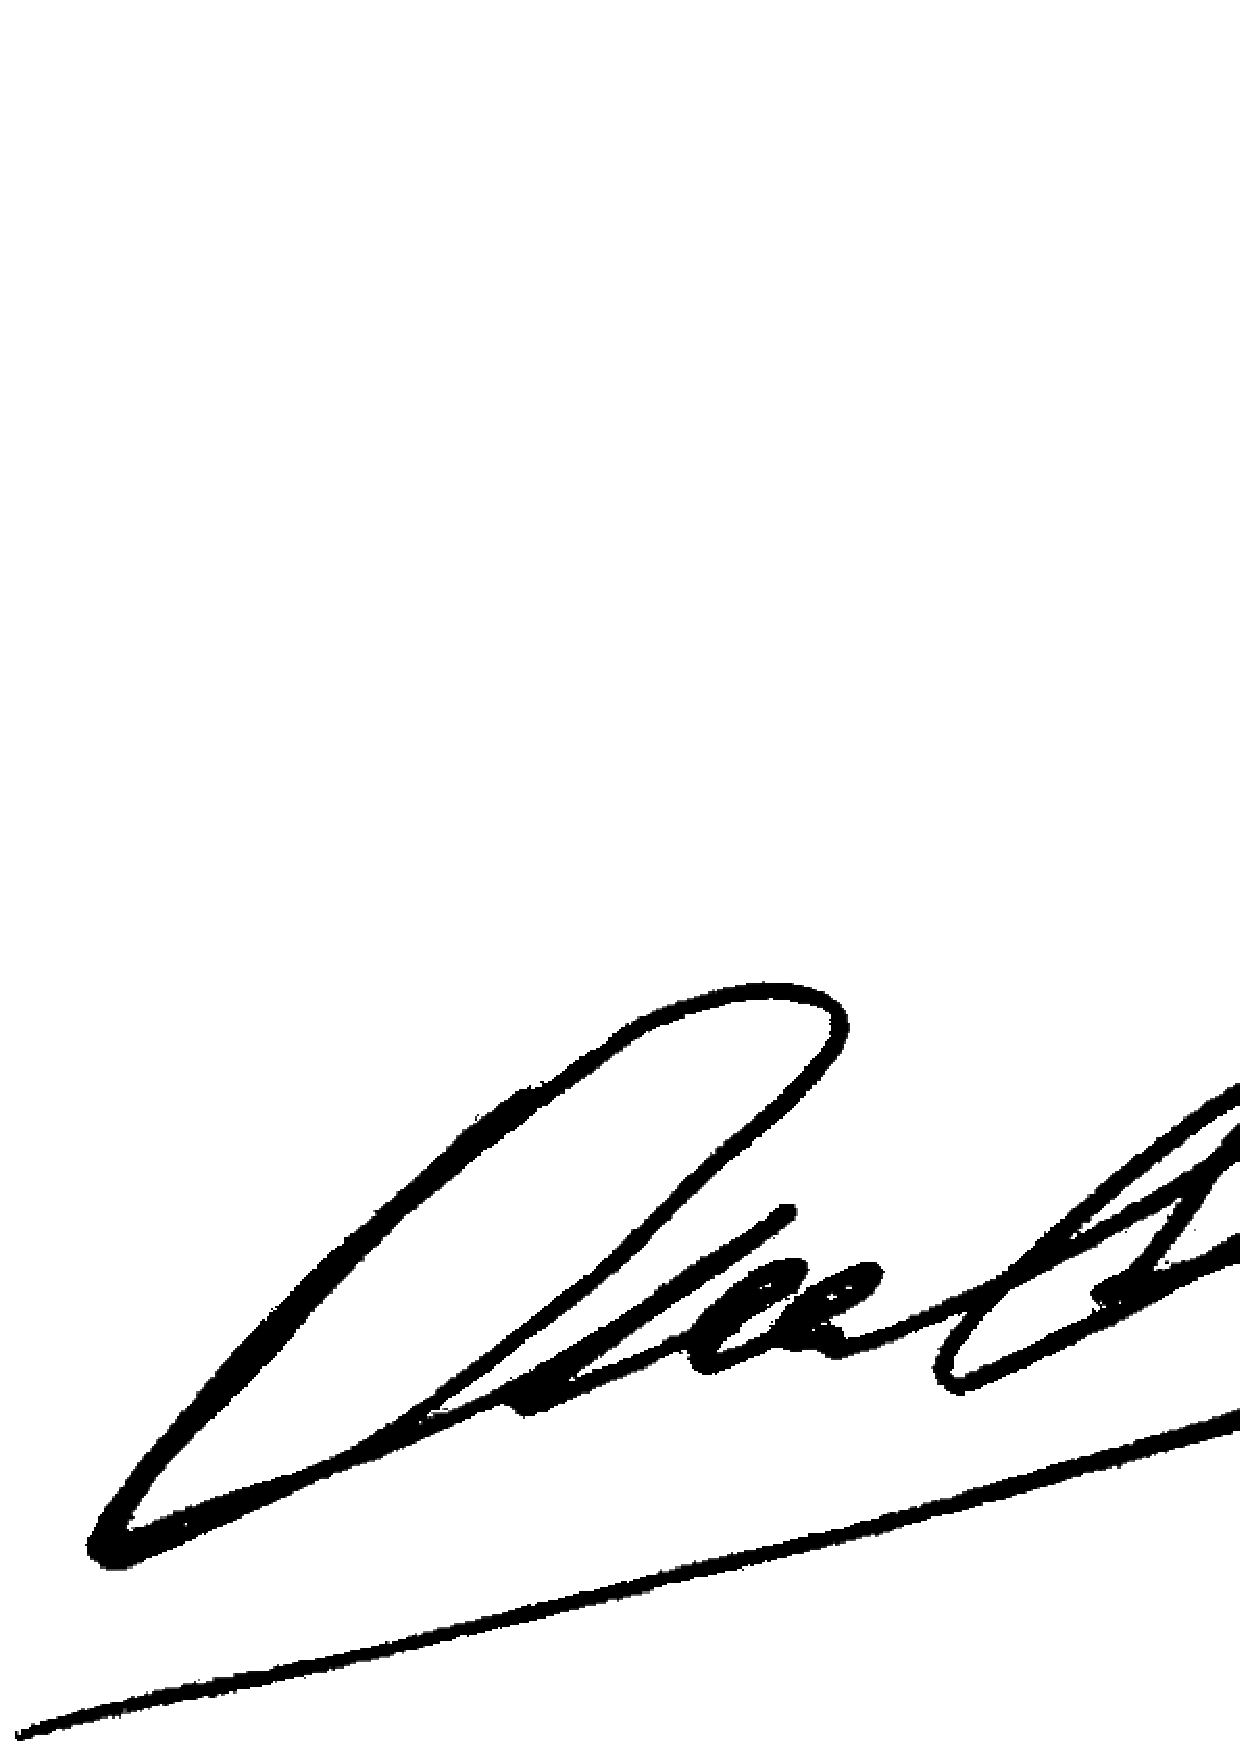
\includegraphics[height=1.5cm]{personal-signature.png}
%        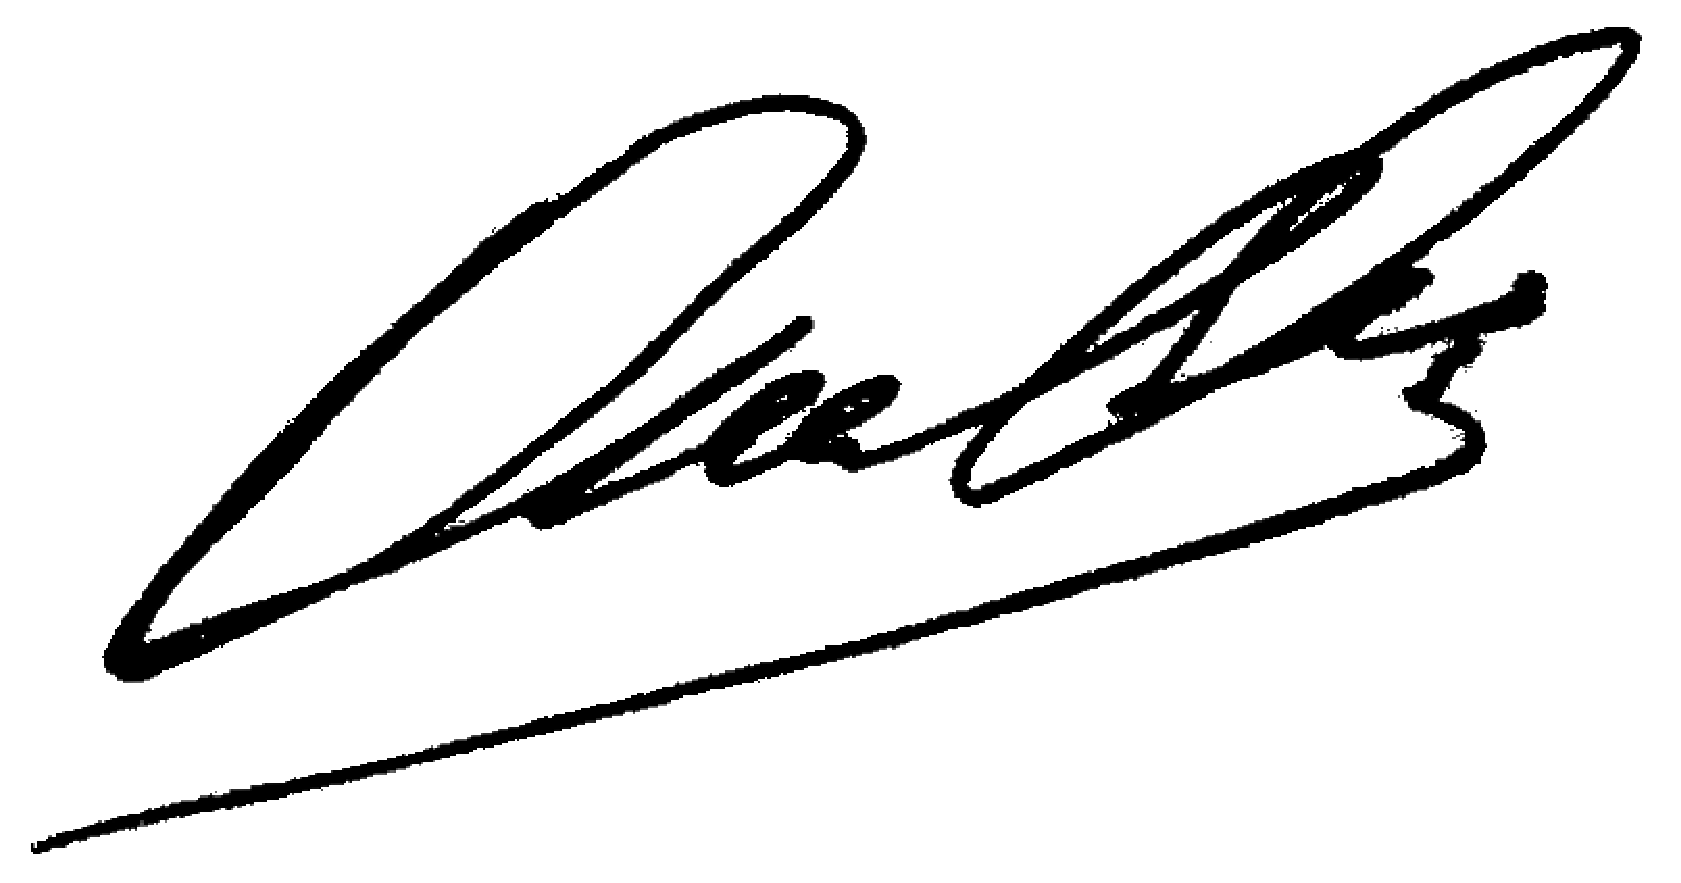
\includegraphics[height=1.5cm]{personal-signature}
%    }\\
\end{tabularx}

\vspace{0pt plus1fill}
\noindent%
\begin{tabularx}{\textwidth}{@{}lXr@{}}%
    & & 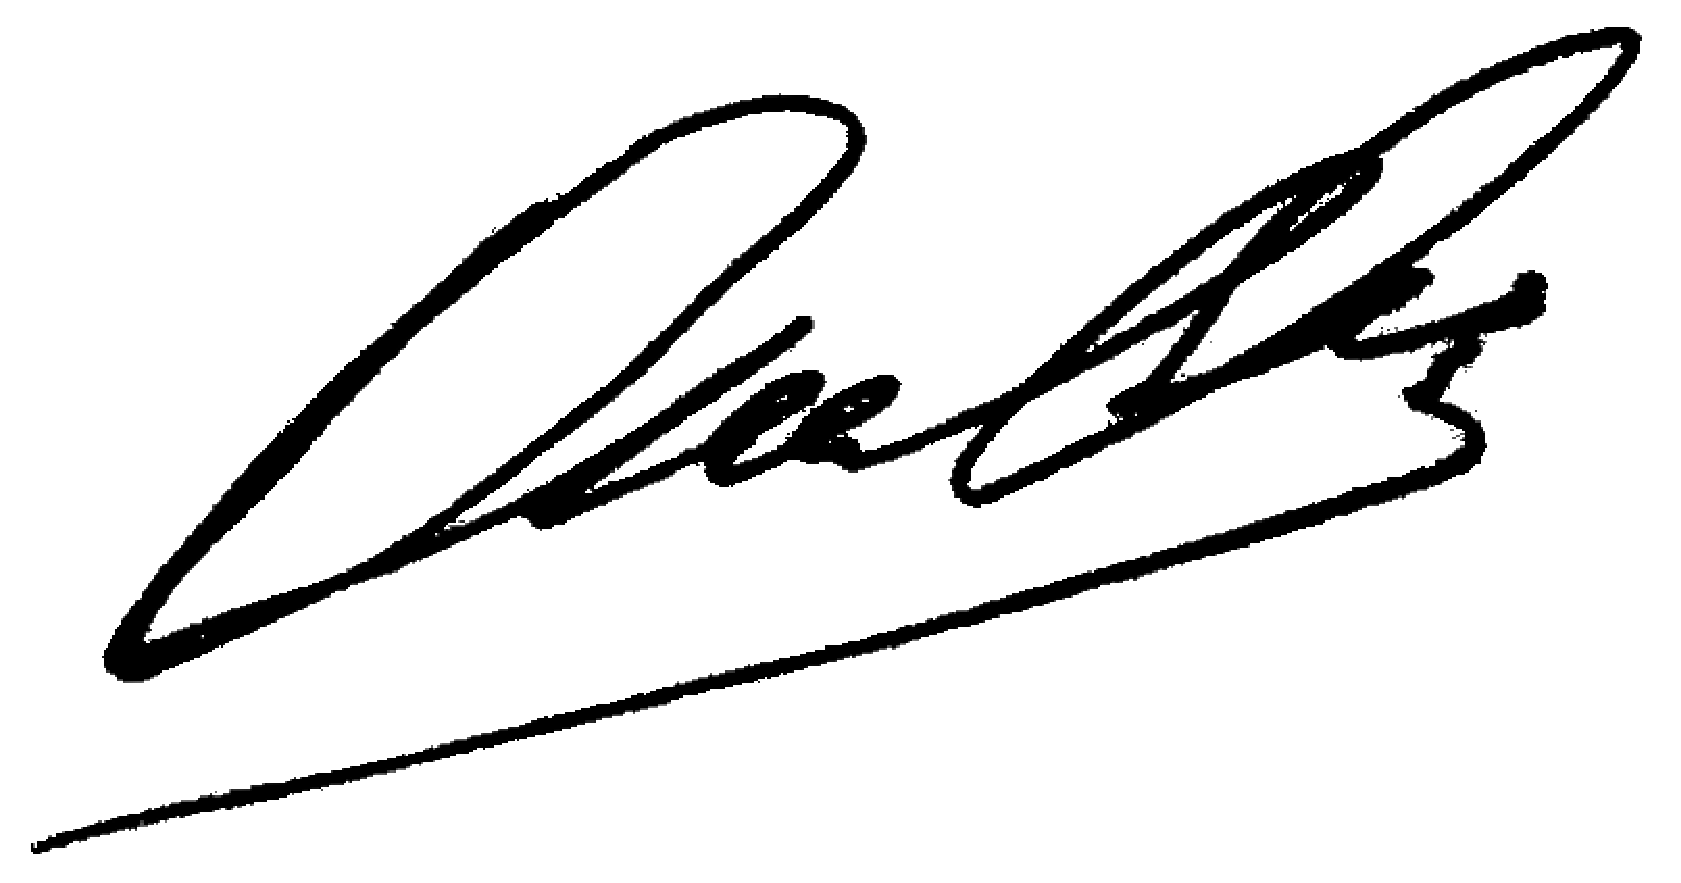
\includegraphics[height=1.5cm]{personal-signature}  %!!!!!!!!!!!!!!!!!!!!!!!!! Olikh
    \\
\end{tabularx}


\vspace{0pt plus-1fill} %число перед fill = кратность относительно некоторого расстояния fill, кусками которого заполнены пустые места
\begin{center}
%\textbf {\large \thesisAuthor}
\textbf {\MakeUppercase{ \thesisAuthor}}
\end{center}

\vspace{0pt plus1fill} %число перед fill = кратность относительно некоторого расстояния fill, кусками которого заполнены пустые места
\begin{flushright}%
  \begin{minipage}[b]{0.4\linewidth}
    \begin{flushleft}%
       УДК \thesisUdk
    \end{flushleft}%
  \end{minipage}
\end{flushright}%

\vspace{0pt plus3fill} %число перед fill = кратность относительно некоторого расстояния fill, кусками которого заполнены пустые места
\begin{center}
\textbf { \MakeUppercase
\thesisTitle}

\vspace{0pt plus3fill} %число перед fill = кратность относительно некоторого расстояния fill, кусками которого заполнены пустые места
%{\large Спеціальність \thesisSpecialtyNumber\ "---\par <<\thesisSpecialtyTitle>>}
{\large Спеціальність \thesisSpecialtyNumber -- \thesisSpecialtyTitle}

\vspace{0pt plus1.5fill} %число перед fill = кратность относительно некоторого расстояния fill, кусками которого заполнены пустые места
\Large{Автореферат}\par
\large{дисертації на здобуття наукового ступеня\par \thesisDegree}
\end{center}

\vspace{0pt plus4fill} %число перед fill = кратность относительно некоторого расстояния fill, кусками которого заполнены пустые места
{\centering\thesisCity~-- \thesisYear\par}

\newpage
% оборотная сторона обложки
\thispagestyle{empty}
\noindent Дисертацією є рукопис.
\vspace{0.008\paperheight plus1fill}

\noindent Робота виконана на кафедрі загальної фізики фізичного факультету {\thesisOfOrganization}.

\vspace{0.008\paperheight plus1fill}
\noindent%
\begin{tabularx}{\textwidth}{@{}lX@{}}
%    Научный руководитель:   & \supervisorRegalia\par
%                              \textbf{\supervisorFio}
%    \vspace{0.013\paperheight}\\
    \textbf{Офіційні опоненти:}  &
    \ifnumequal{\value{showopplead}}{0}{\vspace{13\onelineskip plus1fill}}{%
        \opponentOneRegalia,\par
        \textbf{\opponentOneFio,}\par
        \opponentOneJobPlace,\par
        \opponentOneJobPost\par
        відділу радіаційної фізики \par
            \vspace{0.01\paperheight}
        \opponentTwoRegalia,\par
        \textbf{\opponentTwoFio,}\par
        \opponentTwoJobPlace\par
         НАН України,\par
        \opponentTwoJobPost\par
        напівпровідникової фотоенергетики \par
            \vspace{0.01\paperheight}
        \opponentTreeRegalia,\par
        член--кореспондент НАН України\par
        \textbf{\opponentTreeFio,}\par
        \opponentTreeJobPlace\par
         НАН України,\par
        \opponentTreeJobPost
    }%
%    \vspace{0.013\paperheight} \\
%    Ведущая организация:    &
%    \ifnumequal{\value{showopplead}}{0}{\vspace{6\onelineskip plus1fill}}{%
%        \leadingOrganizationTitle
%    }%
\end{tabularx}
\vspace{0.008\paperheight plus1fill}

\noindent Захист відбудеться \defenseDate~на~засіданні спеціалізованої вченої ради \defenseCouncilNumber~
при \thesisInOrganization~за адресою: \defenseCouncilAddress.

\vspace{0.008\paperheight plus1fill}
\noindent З дисертацією можна ознайомитись у  Науковій  бібліотеці ім.~М.~Максимовича
Київського національного університету імені Тараса Шевченка за адресою: 01033,
Київ, вул. Володимирська,~58
%С диссертацией можно ознакомиться в библиотеке \synopsisLibrary.

%\vspace{0.008\paperheight plus1fill}
%\noindent Отзывы на автореферат в двух экземплярах, заверенные печатью учреждения, просьба направлять по адресу: \defenseCouncilAddress, ученому секретарю диссертационного совета~\defenseCouncilNumber.

\vspace{0.008\paperheight plus1fill}
\noindent{Автореферат розісланий \synopsisDate.}

%\noindent Телефон для справок: \defenseCouncilPhone.

\vspace{0.008\paperheight plus1fill}
\noindent%
\begin{tabularx}{\textwidth}{@{}%
>{\raggedright\arraybackslash}b{18em}@{}
>{\centering\arraybackslash}X
r
@{}}
    Вчений секретар\par
    спеціалізованої вченої ради
    \defenseCouncilNumber,\par
    \defenseSecretaryRegalia
    &
    \ifnumequal{\value{showsecrsign}}{0}{}{%
%        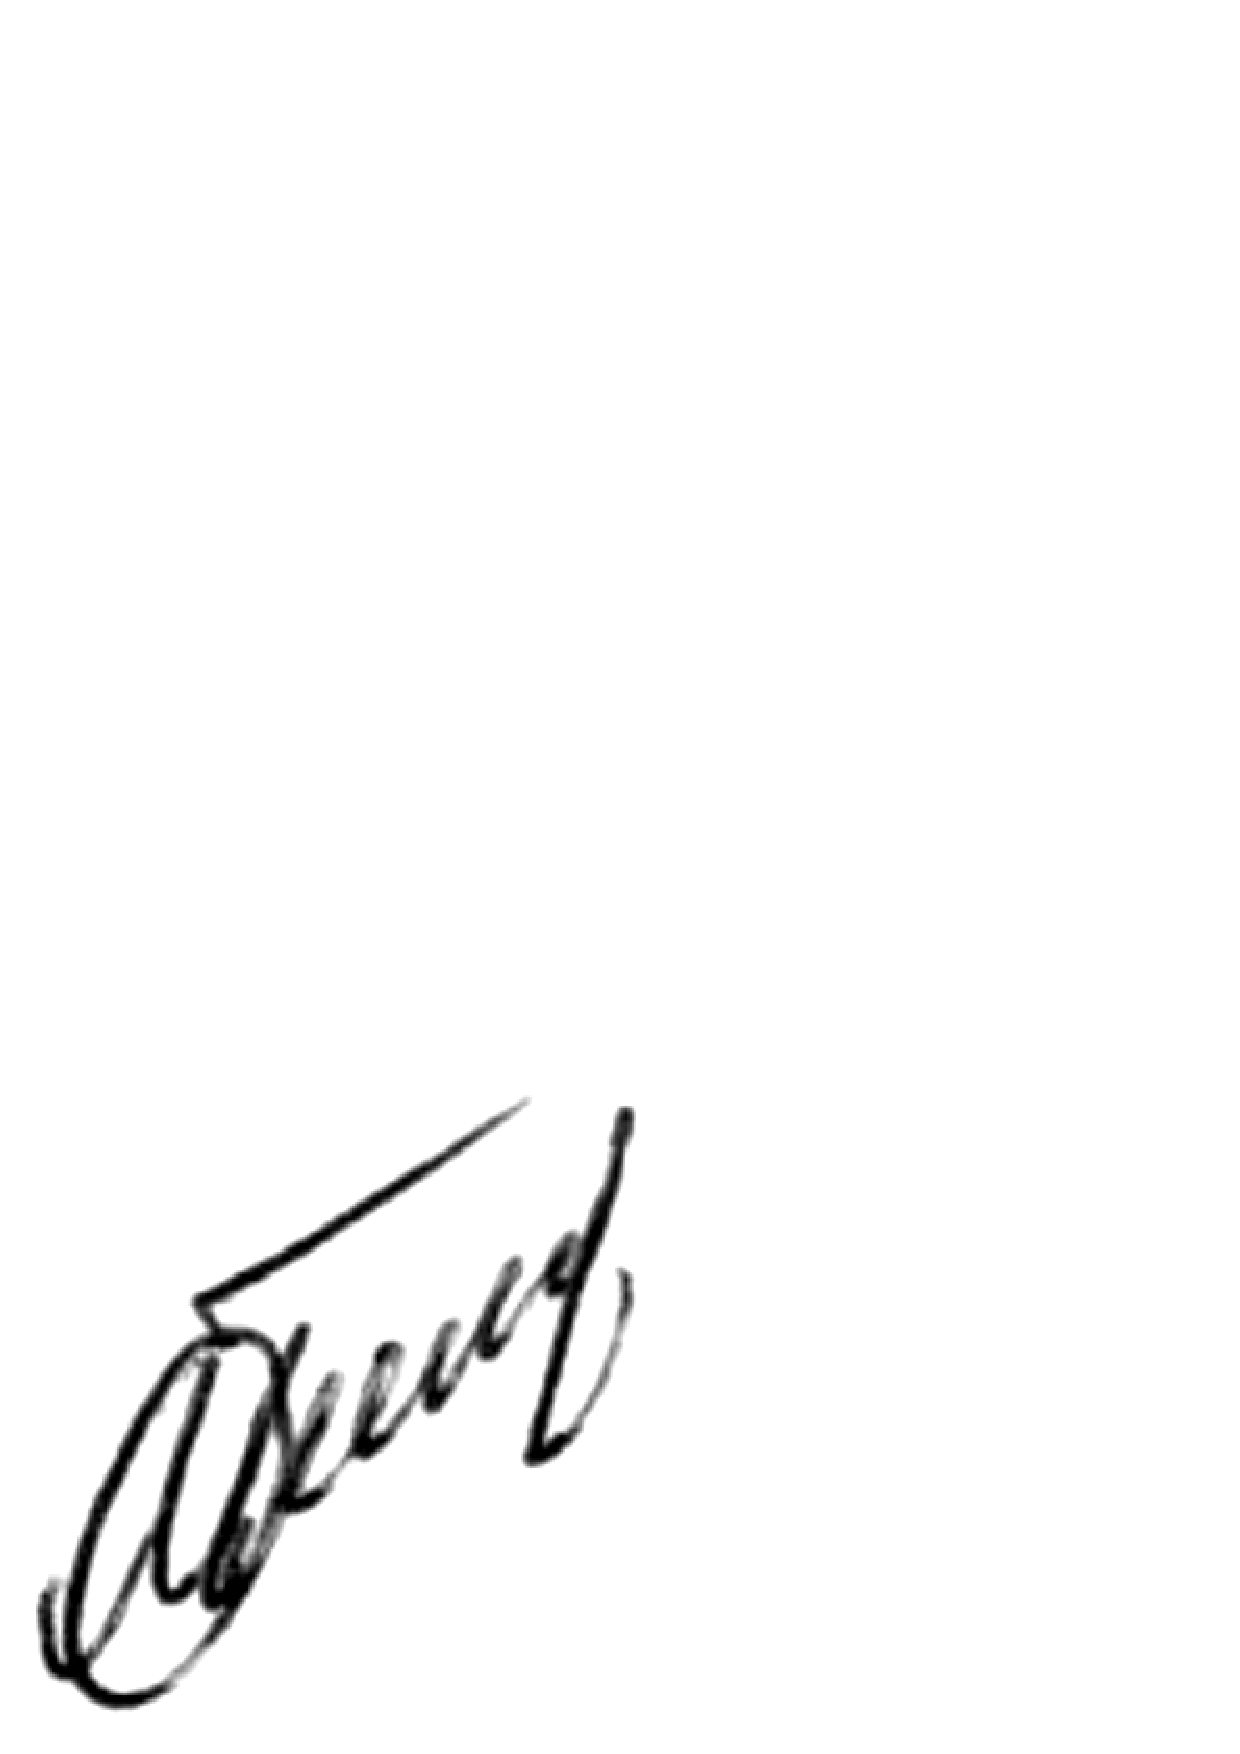
\includegraphics[width=2cm]{secretary-signature.png}%
        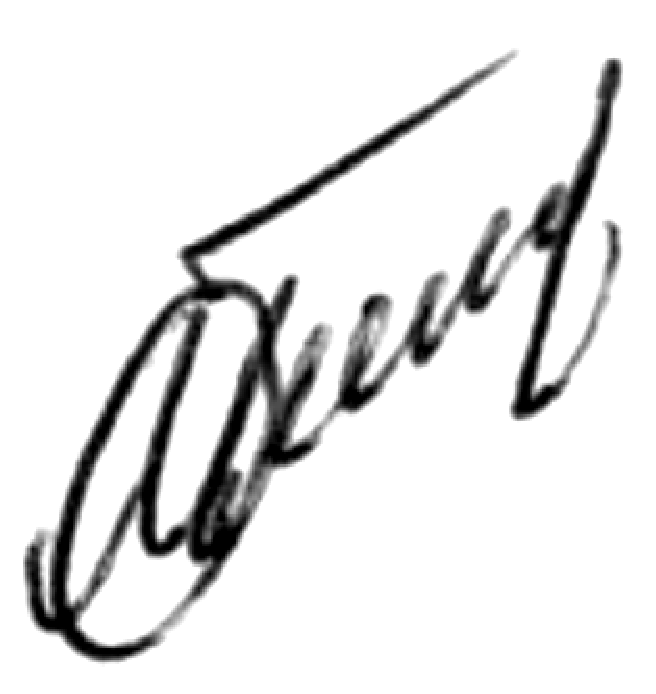
\includegraphics[width=2cm]{secretary-signature}% !!!!!!!!!!!!!! Olikh
    }%
    &
    \defenseSecretaryFio
\end{tabularx}
        % Титульный лист
\mainmatter                   % В том числе начинает нумерацию страниц арабскими цифрами с единицы
%\mainmatter*                  % Нумерация страниц не изменится, но начнётся с новой страницы
%%

%\section*{\MakeUppercase{Загальна характеристика роботи}}
%\section*{\MakeUppercase{
%\textcolor{white}{[1--25]}
%Загальна характеристика роботи
%\textcolor{white}
%{\cite{Olikh2018JAP,Olikh2018SM,Olikh:Ultras2016,Olikh2016JSem,
%Olikh:Rev,OlikhJAP,Olikh:Ultras,Olikh:UPJ2014,
%Olikh:2013IEEE,Olikh:SEMT2013,Olikh:FTP2013,Olikh:UPJ2013,
%Olikh:FTP2011,Olikh:SEMT2011,Olikh:UPJ2010,Gorb2010,Olikh:FTP2009,
%Olikh:SEMT2007,Olikh:MRS2007,Olikh:PZTF2006,
%Olikh:PhChOM2005,Olikh:PJE2004,Olikh:SEMT2004,Olikh:SPQEO2003,
%Olikh:Visn2003,
%1UNCPS,3Tomsk,1SEMST,50IUFFC,9APTTE,2005IUS,ICU2007SC,ICU2007GA,2007MRS,3UNCPS,6DrogGorb,6Drog,
%4UNCPS,4Kremen,7Drog,5UNCPS,2012Ternop,14Plivk,8Drog,2013Buk,6UNCPS,2014IUSOl,2014IUS,6SEMST,
%2015ICU,6CPFCS,7UNCPS,2017MEICS}}}}
%\end{center}%

\begin{center}
\section*{
\textcolor{white}{[1--25]}
\MakeUppercase{Загальна характеристика роботи}
\textcolor{white}
{\cite{Olikh2018JAP,Olikh2018SM,Olikh:Ultras2016,Olikh2016JSem,
Olikh:Rev,OlikhJAP,Olikh:Ultras,Olikh:UPJ2014,
Olikh:2013IEEE,Olikh:SEMT2013,Olikh:FTP2013,Olikh:UPJ2013,
Olikh:FTP2011,Olikh:SEMT2011,Olikh:UPJ2010,Gorb2010,Olikh:FTP2009,
Olikh:SEMT2007,Olikh:MRS2007,Olikh:PZTF2006,
Olikh:PhChOM2005,Olikh:PJE2004,Olikh:SEMT2004,Olikh:SPQEO2003,
Olikh:Visn2003,
1UNCPS,3Tomsk,1SEMST,50IUFFC,9APTTE,2005IUS,ICU2007SC,ICU2007GA,2007MRS,3UNCPS,6DrogGorb,6Drog,
4UNCPS,2009DRIP13,4Kremen,7Drog,5UNCPS,2012Ternop,14Plivk,8Drog,2013Buk,6UNCPS,2014IUSOl,2014IUS,6SEMST,
2015ICU,6CPFCS,7UNCPS,2017MEICS}}
}
\end{center}




%{\actuality} Обзор, введение в тему, обозначение места данной работы в
%мировых исследованиях и~т.\:п., можно использовать ссылки на~другие
%работы\ifnumequal{\value{bibliosel}}{1}{~\autocite{Gosele1999161}}{}
%(если их~нет, то~в~автореферате
%автоматически пропадёт раздел <<Список литературы>>). Внимание! Ссылки
%на~другие работы в разделе общей характеристики работы можно
%использовать только при использовании \verb!biblatex! (из-за технических
%ограничений \verb!bibtex8!. Это связано с тем, что одна
%и~та~же~характеристика используются и~в~тексте диссертации, и в
%автореферате. В~последнем, согласно ГОСТ, должен присутствовать список
%работ автора по~теме диссертации, а~\verb!bibtex8! не~умеет выводить в одном
%файле два списка литературы).
%При использовании \verb!biblatex! возможно использование исключительно
%в~автореферате подстрочных ссылок
%для других работ командой \verb!\autocite!, а~также цитирование
%собственных работ командой \verb!\cite!. Для этого в~файле
%\verb!Synopsis/setup.tex! необходимо присвоить положительное значение
%счётчику \verb!\setcounter{usefootcite}{1}!.
%
%Для генерации содержимого титульного листа автореферата, диссертации
%и~презентации используются данные из файла \verb!common/data.tex!. Если,
%например, вы меняете название диссертации, то оно автоматически
%появится в~итоговых файлах после очередного запуска \LaTeX. Согласно
%ГОСТ 7.0.11-2011 <<5.1.1 Титульный лист является первой страницей
%диссертации, служит источником информации, необходимой для обработки и
%поиска документа>>. Наличие логотипа организации на титульном листе
%упрощает обработку и поиск, для этого разметите логотип вашей
%организации в папке images в формате PDF (лучше найти его в векторном
%варианте, чтобы он хорошо смотрелся при печати) под именем
%\verb!logo.pdf!. Настроить размер изображения с логотипом можно
%в~соответствующих местах файлов \verb!title.tex!  отдельно для
%диссертации и автореферата. Если вам логотип не~нужен, то просто
%удалите файл с логотипом.
%
%\ifsynopsis
%Этот абзац появляется только в~автореферате.
%Для формирования блоков, которые будут обрабатываться только в~автореферате,
%заведена проверка условия \verb!\!\verb!ifsynopsis!.
%Значение условия задаётся в~основном файле документа (\verb!synopsis.tex! для
%автореферата).
%\else
%Этот абзац появляется только в~диссертации.
%Через проверку условия \verb!\!\verb!ifsynopsis!, задаваемого в~основном файле
%документа (\verb!dissertation.tex! для диссертации), можно сделать новую
%команду, обеспечивающую появление цитаты в~диссертации, но~не~в~автореферате.
%\fi
%
%% {\progress}
%% Этот раздел должен быть отдельным структурным элементом по
%% ГОСТ, но он, как правило, включается в описание актуальности
%% темы. Нужен он отдельным структурынм элемементом или нет ---
%% смотрите другие диссертации вашего совета, скорее всего не нужен.
%
%{\aim} данной работы является \ldots
%
%Для~достижения поставленной цели необходимо было решить следующие {\tasks}:
%\begin{enumerate}
%  \item Исследовать, разработать, вычислить и~т.\:д. и~т.\:п.
%  \item Исследовать, разработать, вычислить и~т.\:д. и~т.\:п.
%  \item Исследовать, разработать, вычислить и~т.\:д. и~т.\:п.
%  \item Исследовать, разработать, вычислить и~т.\:д. и~т.\:п.
%\end{enumerate}
%
%
%{\novelty}
%\begin{enumerate}
%  \item Впервые \ldots
%  \item Впервые \ldots
%  \item Было выполнено оригинальное исследование \ldots
%\end{enumerate}
%
%{\influence} \ldots
%
%{\methods} \ldots
%
%{\defpositions}
%\begin{enumerate}
%  \item Первое положение
%  \item Второе положение
%  \item Третье положение
%  \item Четвертое положение
%\end{enumerate}
%В папке Documents можно ознакомиться в решением совета из Томского ГУ
%в~файле \verb+Def_positions.pdf+, где обоснованно даются рекомендации
%по~формулировкам защищаемых положений.
%
%{\reliability} полученных результатов обеспечивается \ldots \ Результаты находятся в соответствии с результатами, полученными другими авторами.
%
%
{\contributionTXT} 
Внесок автора у отримання наукових результатів полягає у постановці задачі роботи
та визначенні методів їх вирішення, виборі об'єктів та формулюванні 
основних напрямків досліджень,
розробці методології експериментальних досліджень.
Переважна більшість експериментальних та теоретичних досліджень виконані автором особисто.
12 з 25 наукових публікацій опублікованих за темою дисертації є одноосібними роботами пошукача.
У наукових працях, опублікованих зі співавторами, автору належить аналіз та узагальнення отриманих
даних, накопичених в результаті проведених досліджень, інтерпретація результатів, участь у написанні наукових статей.



{\probationTXT}
Основні результати, викладені в роботі, доповідались на наукових семінарах
кафедри загальної фізики Київського національного університету імені Тараса Шевченка
і були представлені на наступних наукових конференціях:
І, ІІІ, IV, V, VI та VII Українська наукова конференція з фізики напівпровідників 
(Одеса, Україна, 2002; Одеса, Україна, 2007; Запоріжжя, Україна, 2009;
Ужгород, Україна, 2011; Чернівці, Україна, 2013; Дніпро, Україна, 2016);
III международная конференция <<Радиационно-термические эффекты и процессы в неорганических материалах>> (Томск, Россия, 2002);
1--ша та 6-та Міжнародна науково-технічна конференція <<Сенсорна електроніка і мікросистемні технології СЕМСТ>> (Одеса, Україна, 2004; 2014);
2004 IEEE International Ultrasonics, Ferroelectrics and Frequency Control Joint 50th Anniversary Conference (Montreal, Canada, 2004);
Девятая международная научно--техническая конференция <<Актуальные проблемы твердотельной электроники и микроэлектроники>> (Дивноморское, Россия, 2004);
2005 та 2014 IEEE International Ultrasonics Symposium (Rotterdam, Netherlands, 2005; Chicago, USA, 2014);
2007 та 2015 International Congress on Ultrasonics (Vienna, Austria, 2007; Metz, France, 2015);
MRS 2007 Spring Meeting, Symposium F: Semiconductor Defect Engineering – Materials, Synthetic Structures, and Devices II (San Francisco, USA, 2007);
VІ та VІІ Міжнародна школа-конференція <<Актуальні проблеми фізики напівпровідників>> (Дрогобич, Україна, 2008; 2010);
ХІІ та ХІV Міжнародна конференція <<Фізика і технологія тонких плівок та наносистем>> (Івано--Франківськ, Україна, 2009; Буковель, Україна, 2013);
Четверта міжнародна науково--практична конференція <<Матеріали електронної техніки та сучасні інформаційні технології>> (Кременчук, Україна, 2010);
Всеукраїнська наукова конференція <<Актуальні проблеми теоретичної, експериментальної та прикладної фізики>> (Тернопіль, Україна, 2012);
International research and practice conference <<Nanotechnology and nanomaterials>> (Bukovel, Ukraine, 2013);
IV міжнародна конференція <<Сучасні проблеми фізики конденсованого стану>> (Київ, Україна, 2015);
ІІ Всеукраїнська науково--практична конференція МЕІСS--2017 (Дніпро, Україна, 2017).

{\publicationsTXT}
За отриманими результатами опубліковано 25 наукових праць,
з них 24 статті у фахових журналах і 1 у матеріалах наукової конференції.

{\structureTXT}
Дисертація складається із вступу, шести розділів, загальних висновків та списку використаних джерел.
Загальних обсяг дисертації складає
%% на случай ошибок оставляю исходный кусок на месте, закомментированным
%\ref*{TotPages}~сторінки з~\totalfigures{}~рисунками та~\totaltables{}~таблицями.
%Список використаних джерел містить \total{citenum}~найменувань.
%
\formbytotal{TotPages}{сторінк}{у}{и}{ок}, включаючи
\formbytotal{totalcount@figure}{рисун}{ок}{ки}{ків} та
\formbytotal{totalcount@table}{таблиц}{ю}{і}{ь}.   
%Список використаних джерел містить
%\formbytotal{citenum}{найменуван}{ня}{ь}{ь}.



%
%%\publications\ Основные результаты по теме диссертации изложены в ХХ печатных изданиях~\cite{Sokolov,Gaidaenko,Lermontov,Management},
%%Х из которых изданы в журналах, рекомендованных ВАК~\cite{Sokolov,Gaidaenko},
%%ХХ --- в тезисах докладов~\cite{Lermontov,Management}.
%
%\ifnumequal{\value{bibliosel}}{0}{% Встроенная реализация с загрузкой файла через движок bibtex8
%    \publications\ Основные результаты по теме диссертации изложены в XX печатных изданиях,
%    X из которых изданы в журналах, рекомендованных ВАК,
%    X "--- в тезисах докладов.%
%}{% Реализация пакетом biblatex через движок biber
%%Сделана отдельная секция, чтобы не отображались в списке цитированных материалов
%    \begin{refsection}[vak,papers,conf]% Подсчет и нумерация авторских работ. Засчитываются только те, которые были прописаны внутри \nocite{}.
%        %Чтобы сменить порядок разделов в сгрупированном списке литературы необходимо перетасовать следующие три строчки, а также команды в разделе \newcommand*{\insertbiblioauthorgrouped} в файле biblio/biblatex.tex
%        \printbibliography[heading=countauthorvak, env=countauthorvak, keyword=biblioauthorvak, section=1]%
%        \printbibliography[heading=countauthorconf, env=countauthorconf, keyword=biblioauthorconf, section=1]%
%        \printbibliography[heading=countauthornotvak, env=countauthornotvak, keyword=biblioauthornotvak, section=1]%
%        \printbibliography[heading=countauthor, env=countauthor, keyword=biblioauthor, section=1]%
%        \nocite{%Порядок перечисления в этом блоке определяет порядок вывода в списке публикаций автора
%                vakbib1,vakbib2,%
%                confbib1,confbib2,%
%                bib1,bib2,%
%        }%
%        \publications\ Основные результаты по теме диссертации изложены в~\arabic{citeauthor}~печатных изданиях,
%        \arabic{citeauthorvak} из которых изданы в журналах, рекомендованных ВАК,
%        \arabic{citeauthorconf} "--- в~тезисах докладов.
%    \end{refsection}
%    \begin{refsection}[vak,papers,conf]%Блок, позволяющий отобрать из всех работ автора наиболее значимые, и только их вывести в автореферате, но считать в блоке выше общее число работ
%        \printbibliography[heading=countauthorvak, env=countauthorvak, keyword=biblioauthorvak, section=2]%
%        \printbibliography[heading=countauthornotvak, env=countauthornotvak, keyword=biblioauthornotvak, section=2]%
%        \printbibliography[heading=countauthorconf, env=countauthorconf, keyword=biblioauthorconf, section=2]%
%        \printbibliography[heading=countauthor, env=countauthor, keyword=biblioauthor, section=2]%
%        \nocite{vakbib2}%vak
%        \nocite{bib1}%notvak
%        \nocite{confbib1}%conf
%    \end{refsection}
%}
%При использовании пакета \verb!biblatex! для автоматического подсчёта
%количества публикаций автора по теме диссертации, необходимо
%их~здесь перечислить с использованием команды \verb!\nocite!.
 % Характеристика работы по структуре во введении и в автореферате не отличается (ГОСТ Р 7.0.11, пункты 5.3.1 и 9.2.1), потому её загружаем из одного и того же внешнего файла, предварительно задав форму выделения некоторым параметрам

{\structureTXT}
Дисертація складається із вступу, шести розділів, загальних висновків та списку використаних джерел.
Загальних обсяг дисертації становить
367 сторiнок, включаючи 124 рисунки та 31 таблицю.
Список використаних джерел містить 657 найменувань.

%Диссертационная работа была выполнена при поддержке грантов ...

%\underline{\textbf{Объем и структура работы.}} Диссертация состоит из~введения, четырех глав, заключения и~приложения. Полный объем диссертации \textbf{ХХХ}~страниц текста с~\textbf{ХХ}~рисунками и~5~таблицами. Список литературы содержит \textbf{ХХX}~наименование.

%\newpage
\begin{center}
\section*{\MakeUppercase{ОСНОВНИЙ ЗМІСТ РОБОТИ}}
\end{center}

У  \underline{\textbf{вступі}}  обґрунтовано актуальність  вибраної  теми, сформульовано  мету  і
завдання  дослідження, показано  наукову  новизну  та практичну  значимість
отриманих результатів, а також надано інформацію стосовно зв’язку роботи з науковими темами, апробації результатів та
особистого внеску здобувача.

%\begin{center}
%{\textbf{\MakeUppercase{ОСНОВНИЙ ЗМІСТ РОБОТИ}} }
%\end{center}

У  \underline{\textbf{першому розділі}}   стисло проаналізовані основні роботи, присвячені
дослідженням взаємодії пружних хвиль з дефектами у напівпровідникових кристалах.
Підкреслено, що високоінтенсивні акустичні хвилі (АХ) здатні стимулювати дифузію, перебудову та генерацію точкових дефектів у бінарних та однокомпонентних напівпровідникових кристалах, гетеросистемах та бар'єрних пристроях на їх основі,
що, в свою чергу, є причиною залишкових змін електричних, механічних, оптичних та  люмінесцентних властивостей.
Ультразвукова обробка (УЗО) радіаційномодифікованих кристалів та структур може викликати часткове відновлення деградованих властивостей внаслідок низькотемпературного акустовідпалу.
З іншого боку вказано, що дані про вплив опромінення на акусто--дефектну взаємодію в літературі відсутні.
Дослідження особливостей поширення АХ та акустоелектронної взаємодії дозволяє характеризувати як власні, так і домішкові дефекти.
Ультразвук (УЗ) може використовуватися як додатковий позитивний фактор впливу під час різноманітних технологічних  операціях, зокрема при іонній імплантації.
Виявлено, що під час поширення пружних хвиль в напівпровідникових кристалах та приладах на їх основі виникає чимало різноманітних оптичних та електрофізичних ефектів, причиною яких вважається коливальний рух дислокацій чи дія п'єзоелектричного поля.
Водночас підкреслено,
що на початок даної роботи динамічні акустоіндуковані ефекти в бар'єрних структурах на основі неп'єзоелектричних малодислокаційних напівпровідників фактично не досліджувалися.

У  \underline{\textbf{другому розділі}} представлені результати експериментальних досліджень вперше виявлених оборотних акустоіндукованих (АІ) ефектів у радіаційно опромінених та неопромінених кремнієвих структурах з  $p$--$n$ переходом (сонячних елементах, КСЕ).

На початку представлені методики дослідження параметрів бар'єрних структур за умов ультразвукового навантаження (УЗН),
зокрема зосереджено увагу на схемі експерименту, яка унеможливлювала проникненню п'єзоелектричного поля у зразок (рис.~\ref{USL_SC}), методи визначення параметрів АХ та режими УЗН.


\begin{figure}[ht]
\center
%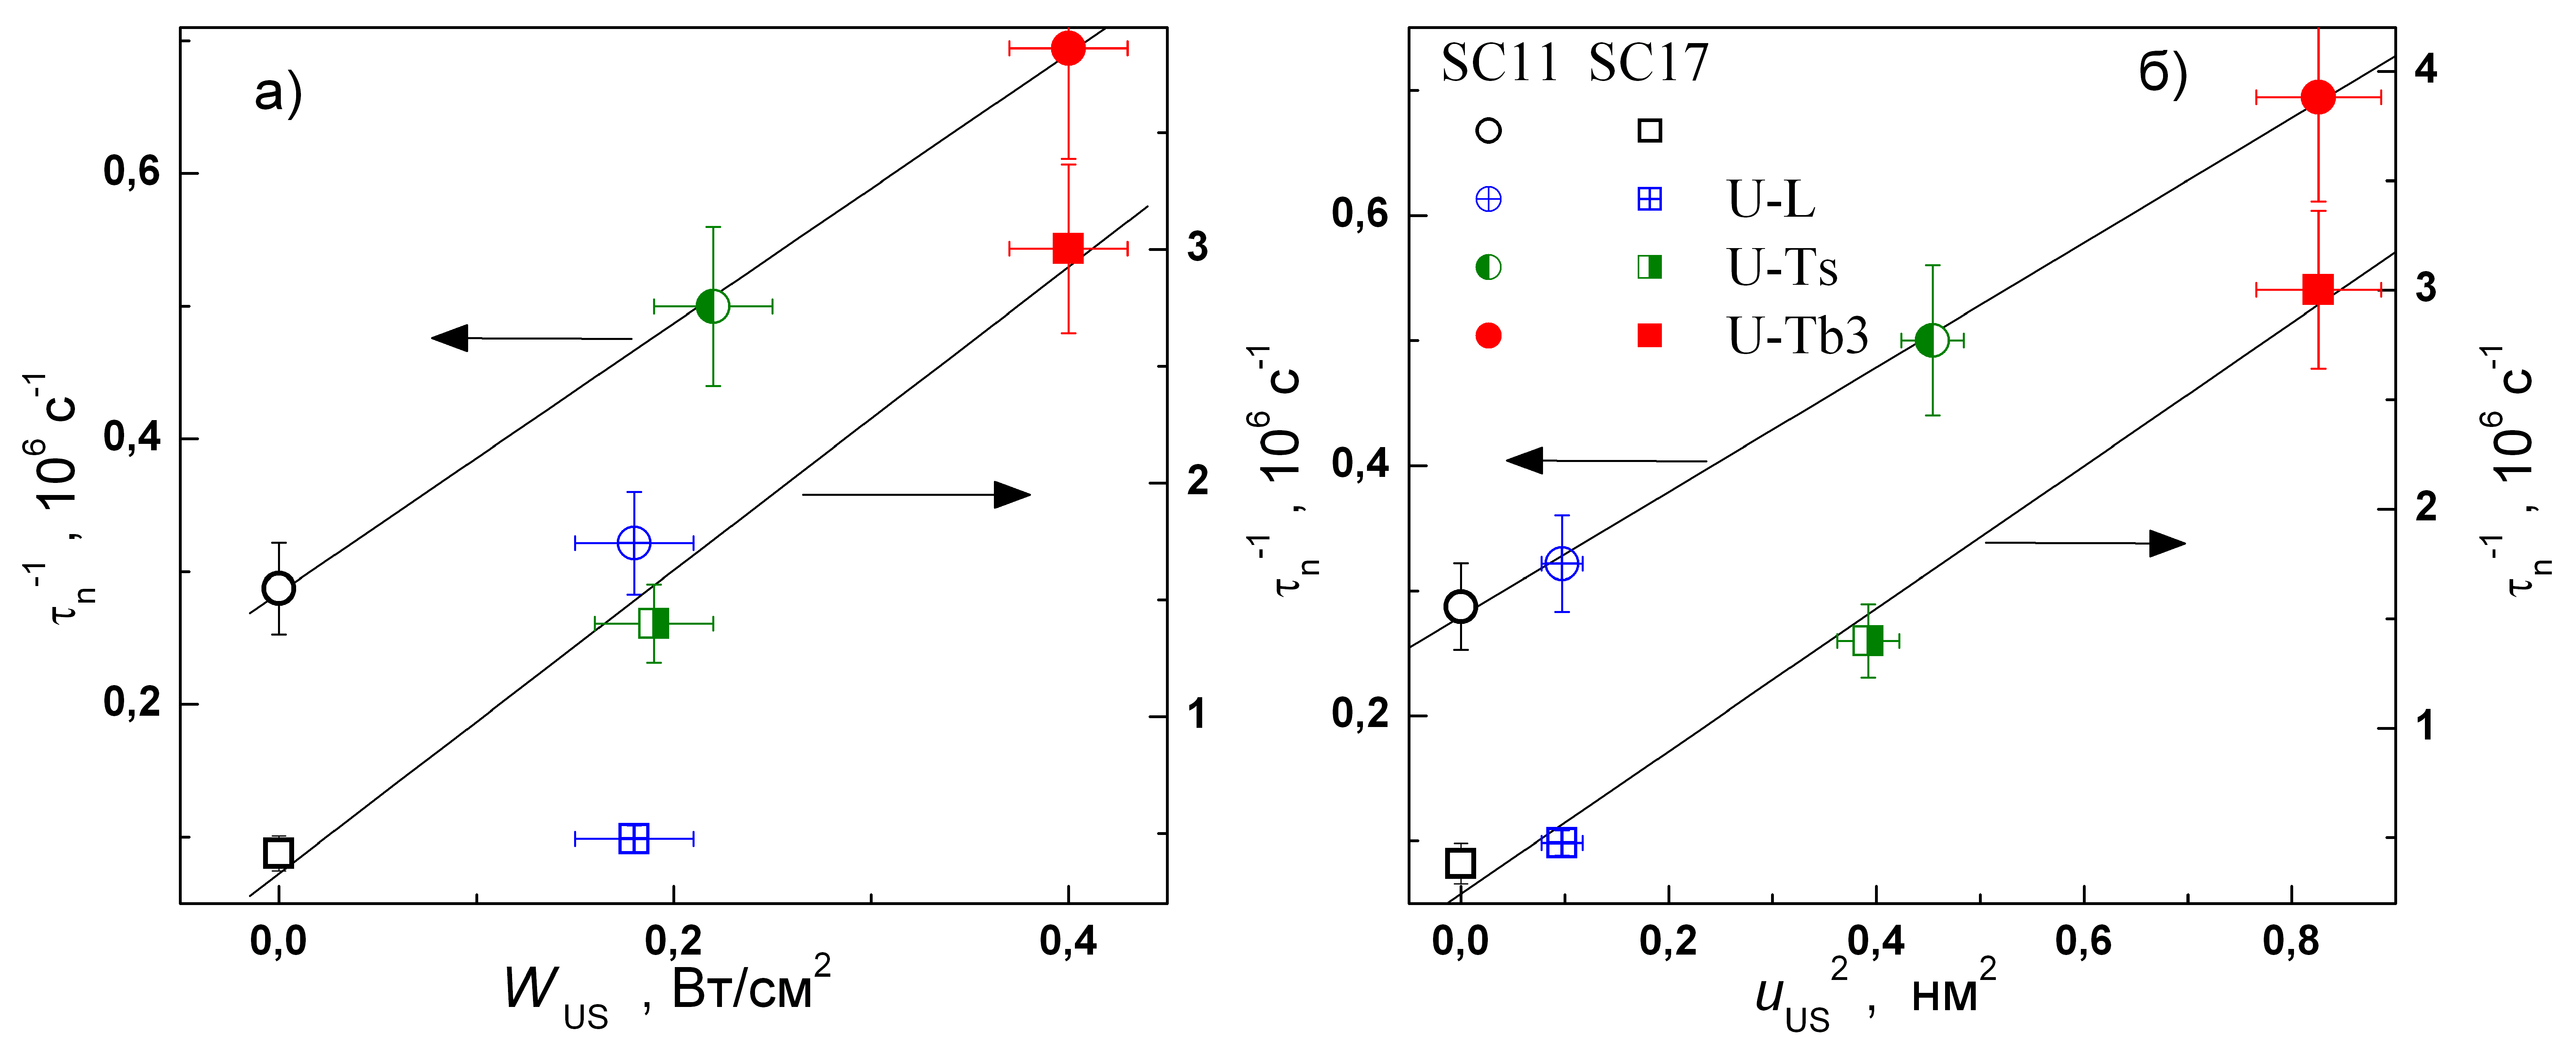
\includegraphics[width=1\textwidth]{figKus}%
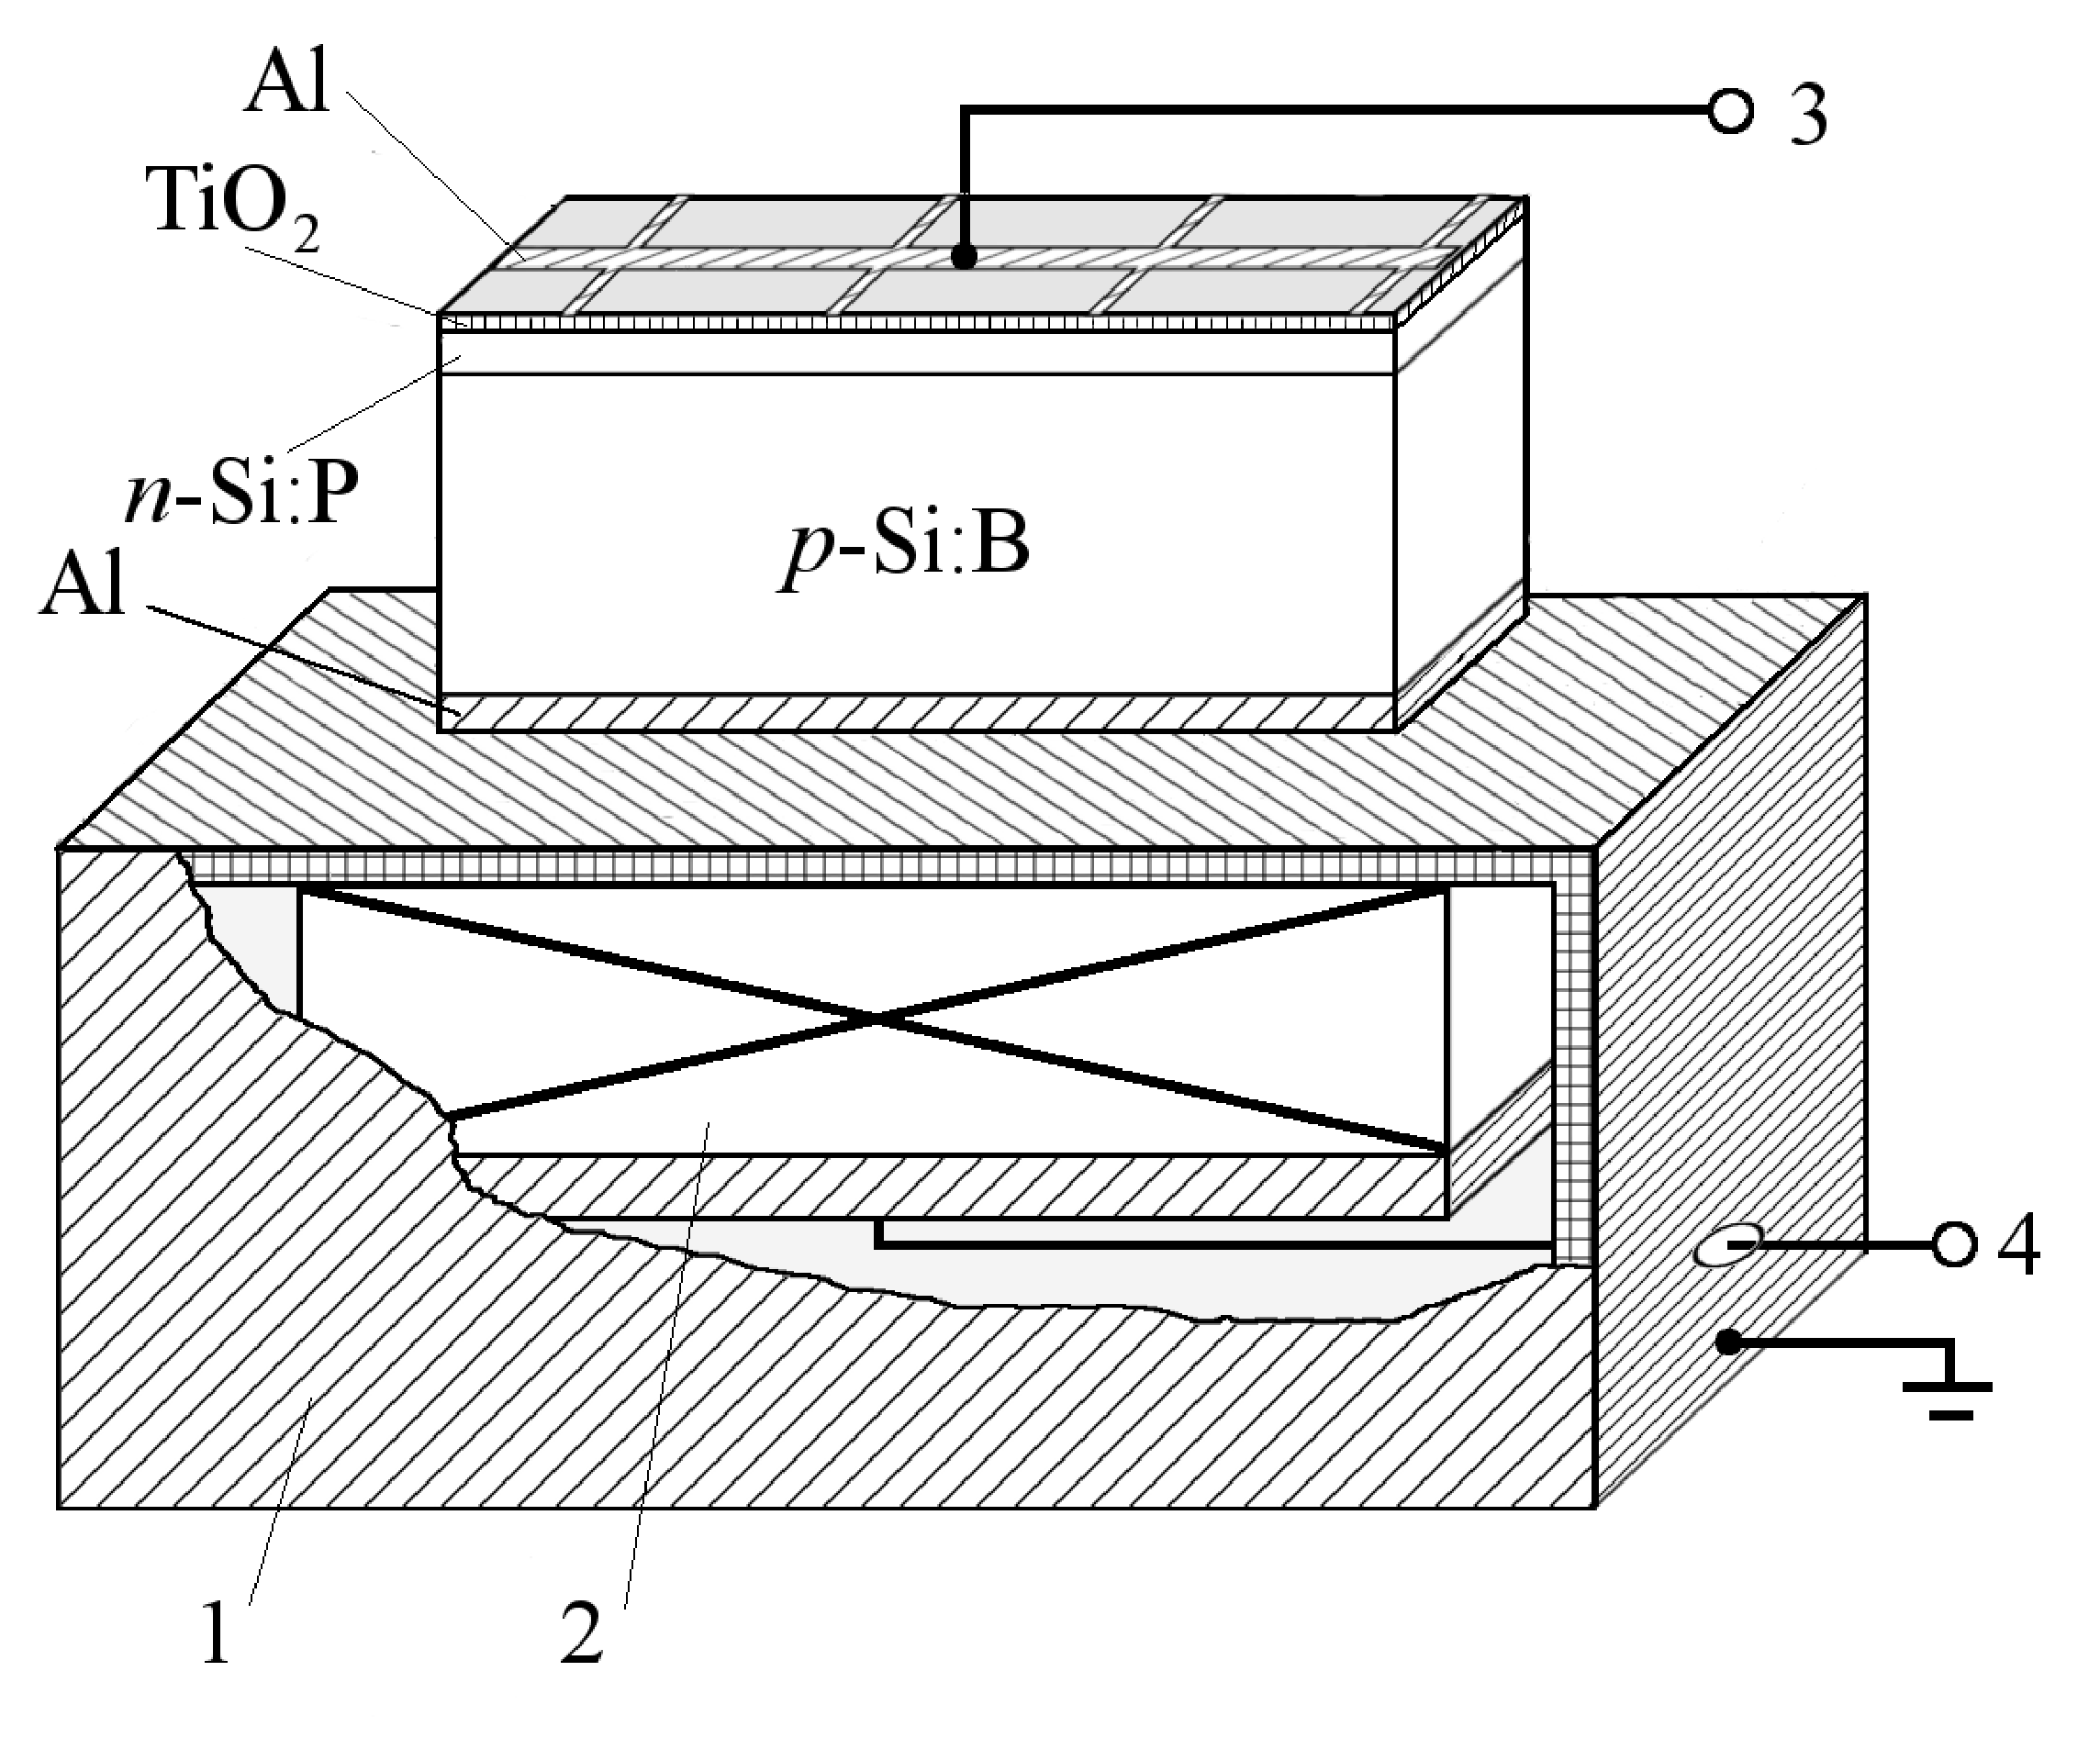
\includegraphics[width=0.4\textwidth]{USL_SC} \hfill
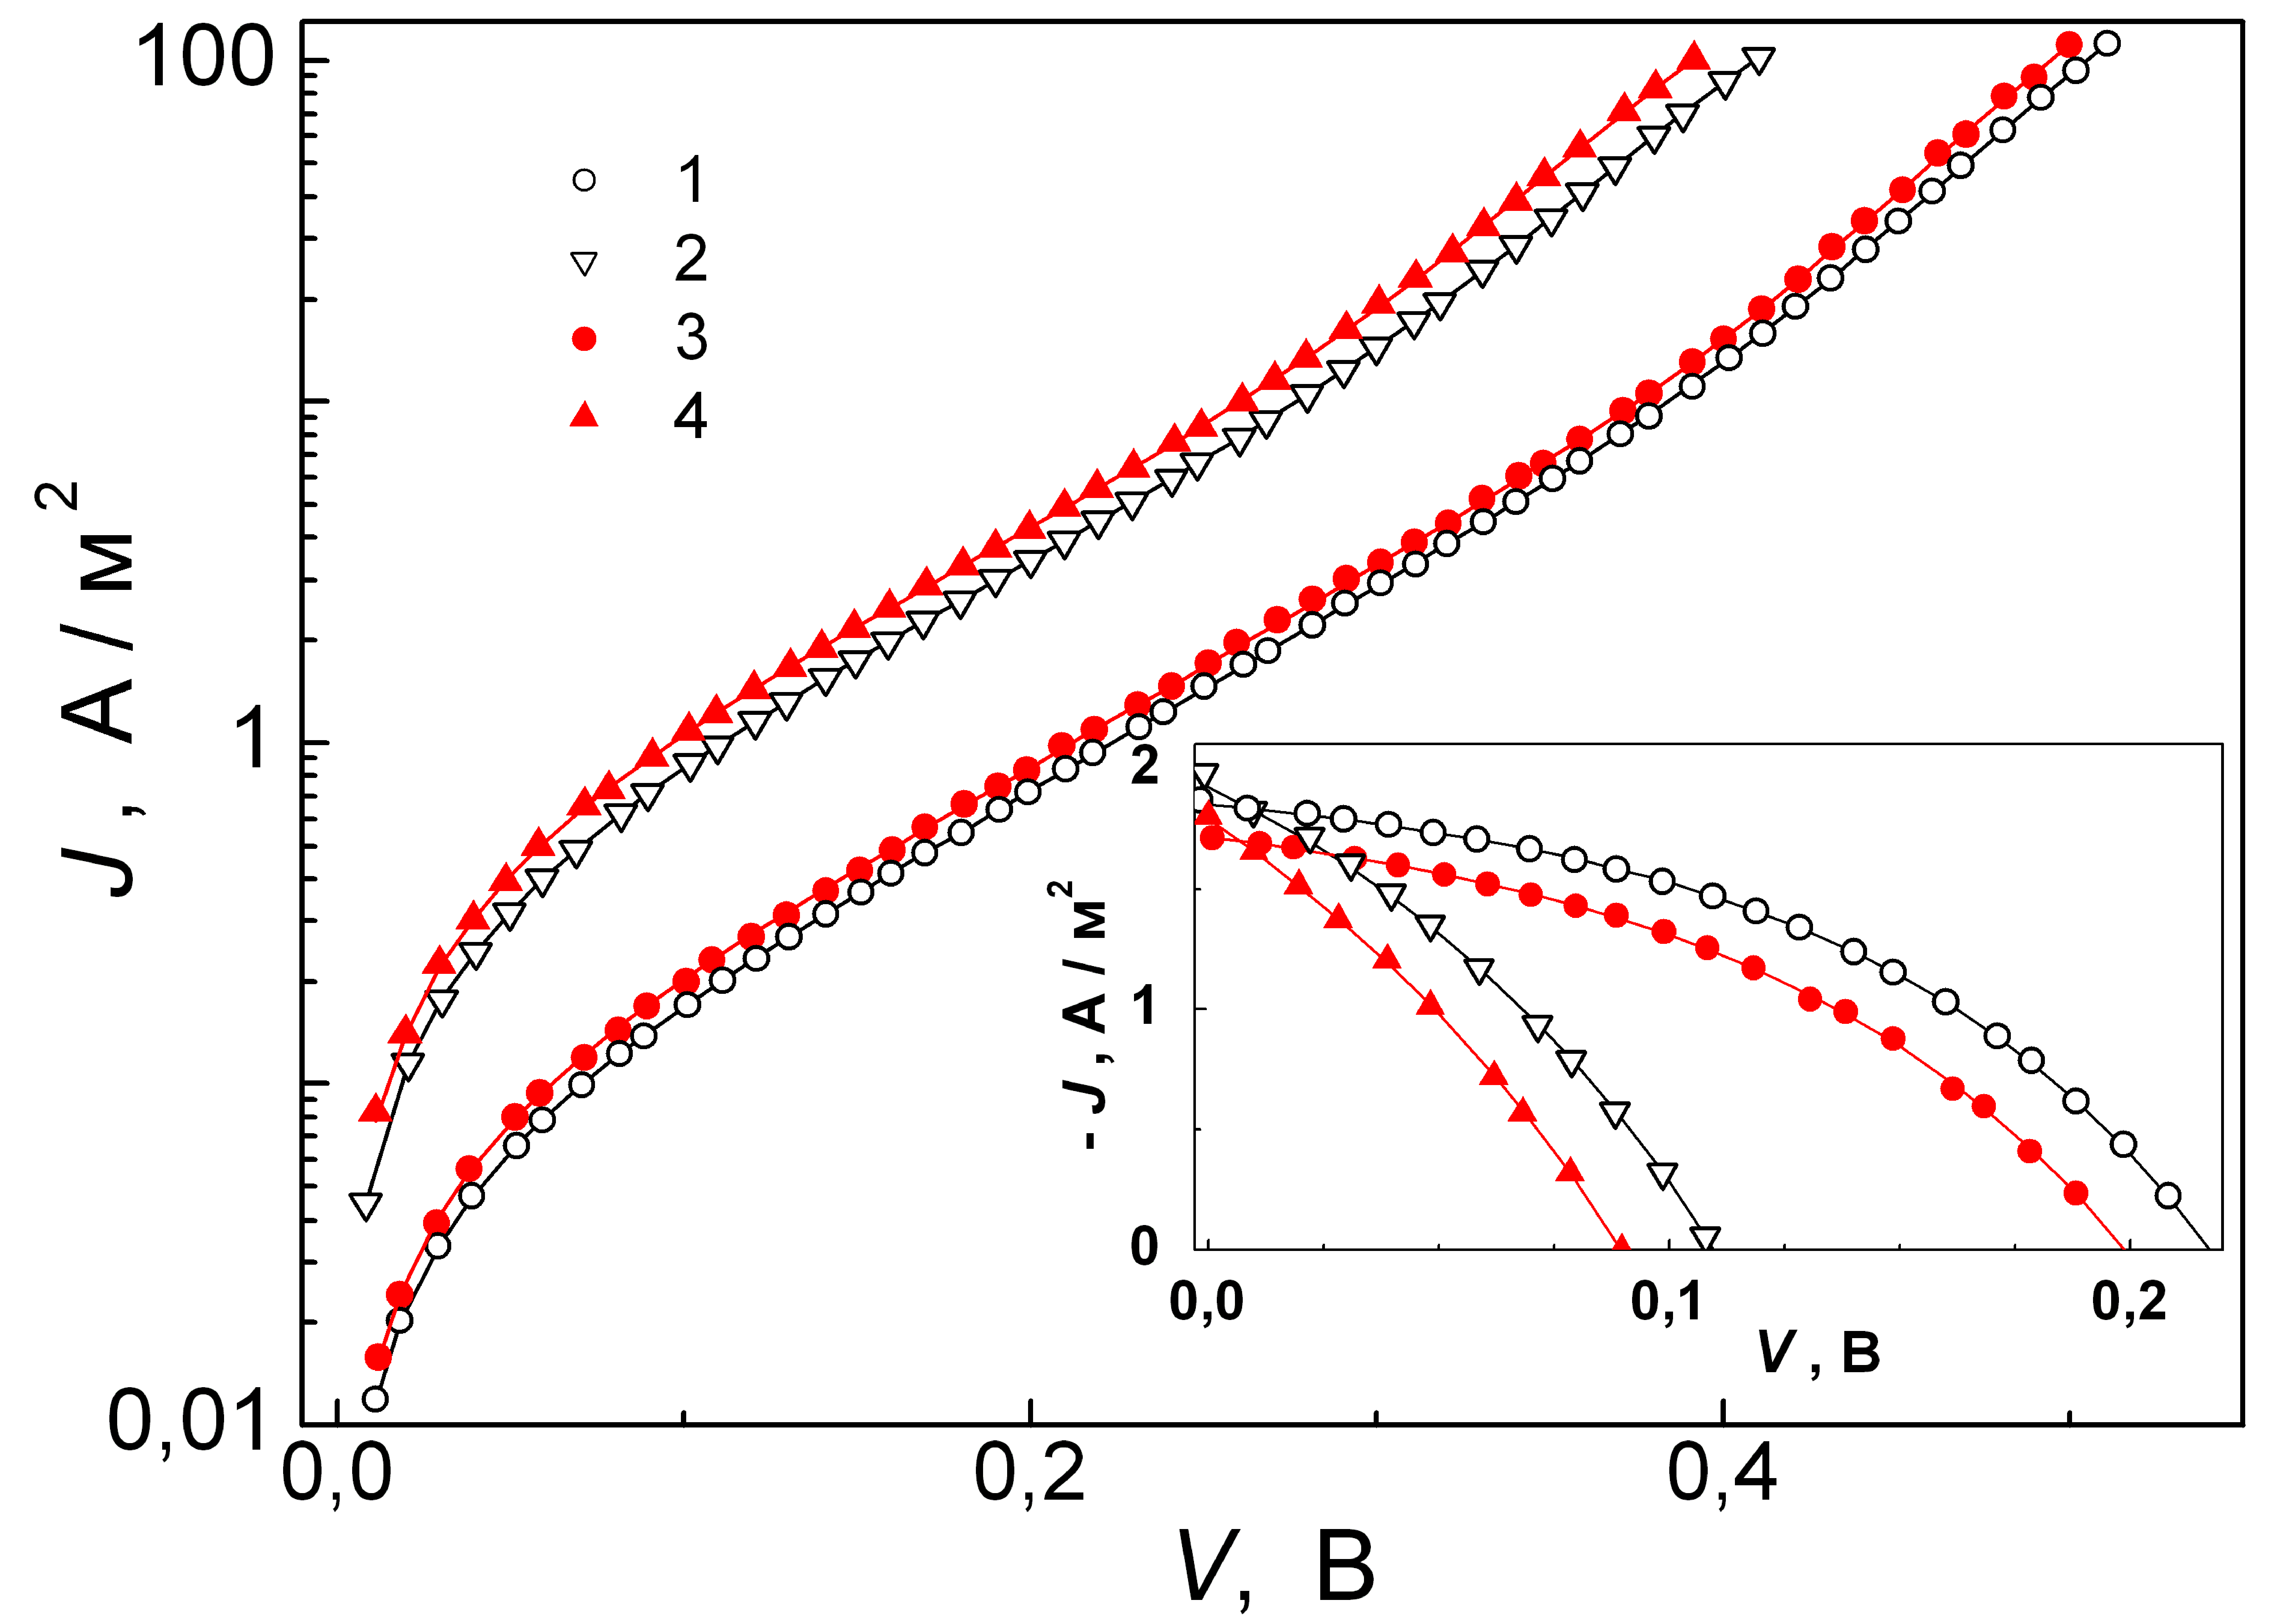
\includegraphics[width=0.55\textwidth]{figSSCIV}
\caption{\label{USL_SC}
Зліва --- схема УЗН.
1 --  екран (алюмінієва фольга, товщина 0,012 мм);
2 --- п'єзоелектричний перетворювач (LiNbO$_3$);
3 --- контакти для вимірювання ВАХ;
4 --- контакти для збудження УЗ.
Справа --- типові ВАХ, виміряні при температурах 301~K (криві 1 та 2, кола) та 341~K (2 та 4, трикутники)
за умов УЗН (2, 4, заповнені точки) та для ненавантаженого зразка (1 та 3, порожні точки)
Точки --- результати вимірів, лінії отримані шляхом апроксимації за формулою (\ref{eqSSCIV})
}%
\end{figure}

Експериментально виявлено, що в діапазоні $290\div340$~К при поширенні УЗ (частота $f_\mathtt{US}=4\div8$~МГц, інтенсивність $W_\mathtt{US}\leq0,4$~Вт/см$^2$) в неопромінених КСЕ відбувається деградація
фотоелектричних властивостей:
спостерігається зменшення густини струму короткого замикання $J_{sc}$ (до 10\%), напруги холостого ходу $V_{oc}$ (до 15\%) та фактори форми ВАХ $F\!F$ (до 5\%).
Зміни оборотні, значення параметрів  після припинення УЗН  та витримки зразків при кімнатній температурі протягом доби повертаються до своїх вихідних значень.
Величини АІ змін слабко залежать від температури, водночас при використанні поперечних АХ зменшення параметрів більш суттєві, ніж у випадку поширення в КСЕ повздовжніх хвиль з такою  $W_\mathtt{US}$.
Останнє свідчить про те, що ефективність впливу УЗ визначається насамперед зміщеннями атомів (деформацією ґратки), а не загальною енергією коливань під час УЗН.


З метою встановлення фізичного механізму виявлених ефектів проведені дослідження поведінки електрофізичних параметрів КСЕ за умов УЗН.
Визначення параметрів проводилось шляхом апроксимації виміряних вольт--амперних характеристик (ВАХ) згідно з моделлю подвійного діоду:

\begin{eqnarray}
\label{eqSSCIV}
\nonumber J(V,\,T)&=&-J_{ph}+\frac{qn_id}{2\tau_{g}}\left\{\exp \left[\frac{q(V-JR_s)}{n_\mathrm{id}kT}\right]-1\right\}+\\
&&+\frac{qn_i^2}{p_p}\sqrt{\frac{\mu_nkT}{\tau_n}}\left\{\exp \left[\frac{q(V-JR_s)}{kT}\right]-1\right\}+\frac{V-JR_s}{R_{sh}}\,,
\end{eqnarray}
де
$J$ --- густина струму,
$V$ --- прикладена напруга,
$J_{ph}$ --- густина фотогенерованого струму,
$n_i$ --- концентрація власних носіїв заряду,
$\tau_{g}$  --- ефективний час життя носіїв заряду в області просторового заряду (ОПЗ),
$d$ --- товщина ОПЗ,
$p_p$ --- концентрація основних носіїв заряду в $p$--області,
%$E_g$ --- ширина забороненої зони напівпровідника,
%$N_c$ та $N_v$ --- ефективна густина станів поблизу дна зони провідності та вершини валентної зони, відповідно;
$n_\mathrm{id}$ --- фактор неідеальності
$R_s$ та $R_{sh}$ --- послідовний та шунтуючий опори, відповідно;
$\mu_n$ та $\tau_n$ --- рухливість та час життя неосновних носіїв в базі діоду.
При апроксимації з використанням методу диференційної еволюції (рис.~\ref{USL_SC}) враховувались температурні та польові залежності $n_i$,
$d$, $\mu_n$, величини  $\tau_g$, $\tau_n$, $n_{\mathrm{id}}$, $R_{sh}$, $R_s$ та  $J_{ph}$ розглядалися як невідомі (шукані).
Крім того, оцінка $\tau_n$ проводилася по температурній залежності струму короткого замикання.

Величини $n_\mathrm{id}$ та $\tau_g$ пов'язані з рекомбінацією в ОПЗ.
Виявлені температурні залежності фактора неідеальності та часу життя в ОПЗ
($n_{\mathrm{id}}(T) \sim T_{\mathrm{id}}/T$,
$\tau_{g}(T)\sim\exp\left(-E_{\tau g}/kT\right)$,
де $T_{\mathrm{id}}$ та $E_{\tau g}$ певні характерні величини),
а також їх абсолютні значення ($n_{\mathrm{id}}>2$, $\tau_{g}\approx(10^{-8}\div10^{-7})$~c),
свідчать, що для опису процесів у досліджуваних структурах доцільно застосовувати модель рекомбінації в системі спарених рівнів двох окремих дефектів (CDLR, coupled defect level recombination)
%\cite{CDLR:JAP}
[1$^*$].
УЗН викликає оборотне зростання $n_\mathrm{id}$  (до 0,04) та зменшення $\tau_g$ (до 30\%).
Оборотність АІ змін та незмінність $T_{\mathrm{id}}$ і $E_{\tau g}$ при поширенні АХ показують, що
при УЗН не відбуваються ні перебудова рекомбінаційних центрів (РЦ), ні зменшення їх концентрації.
Дослідження та оцінки показали, що рекомбінація в квазі--нейтральній області може бути описана в рамках моделі Шоклі--Ріда--Хола (SRH), при цьому $\tau_n^{-1}=\sum_i N_{d,i}\,\,\sigma_{n,i}\,\upsilon_{\mathrm{th},n}$
(де
кількість доданків в сумі визначається загальним числом різних РЦ,
кожний з яких характеризуються концентрацією $N_{d,i}$ та поперечним перерізом захоплення (ППЗ) електронів $\sigma_{n,i}$;
$\upsilon_{\mathrm{th},n}$ --- теплова швидкість електронів).
При УЗН спостерігається достатньо значне (до 90\%) зменшення $\tau_n$, причому
$\tau_{n}^{-1}\sim u_\mathtt{US}^2$ (де $u_\mathtt{US}$ --- амплітуда зміщень атомів при поширенні УЗ).

Було проведено дослідження впливу інтенсивного ($\sim2000$~Вт/м$^2$) довготривалого ($\sim15$~год) освітлення на параметри КСЕ.
Аналіз залишкових змін та перехідних процесів після припинення освітлення показав, що дефектами в ОПЗ та КНО, які приймають участь як у рекомбінаційних процесах, так у акусто--дефектнiй взаємодiї є, переважно, кисневмiснi преципiтати (КП).
Крім того, певний внесок у ці процеси пов'язаний з парами Fe$_i$B$_s$.

Для пояснення виявлених ефектів запропонована модель акустоактивного комплексного РЦ, який складається
з двох дефектів донорного та акцепторного типів (рис.~\ref{fig_Model}) у випадку CDLR  чи є точковим дефектом--комплексом з нееквівалентних компонент у випадку механізму SRH.
При поширенні УЗ на точковий дефект дії періодична сила, амплітуда якої залежить від зміни об'єму кристалу, що припадає на один дефект $\Delta\Omega_d$
%\cite{MirzadeJAP2011}
[2$^*$].
В рамках запропонованої моделі за умов УЗН компоненти РЦ здійснюють гармонічні коливання, частота та вісь яких визначаються акустичною хвилею, тоді як амплітуди та фази залежить також і від  $\Delta\Omega_d^\mathtt{D}$ та
$\Delta\Omega_d^\mathtt{A}$ кожної з них.
При цьому відстань між цими компонентами в умовах УЗН $r_\mathtt{US}$ залежить від часу

\begin{figure}[ht]
\center
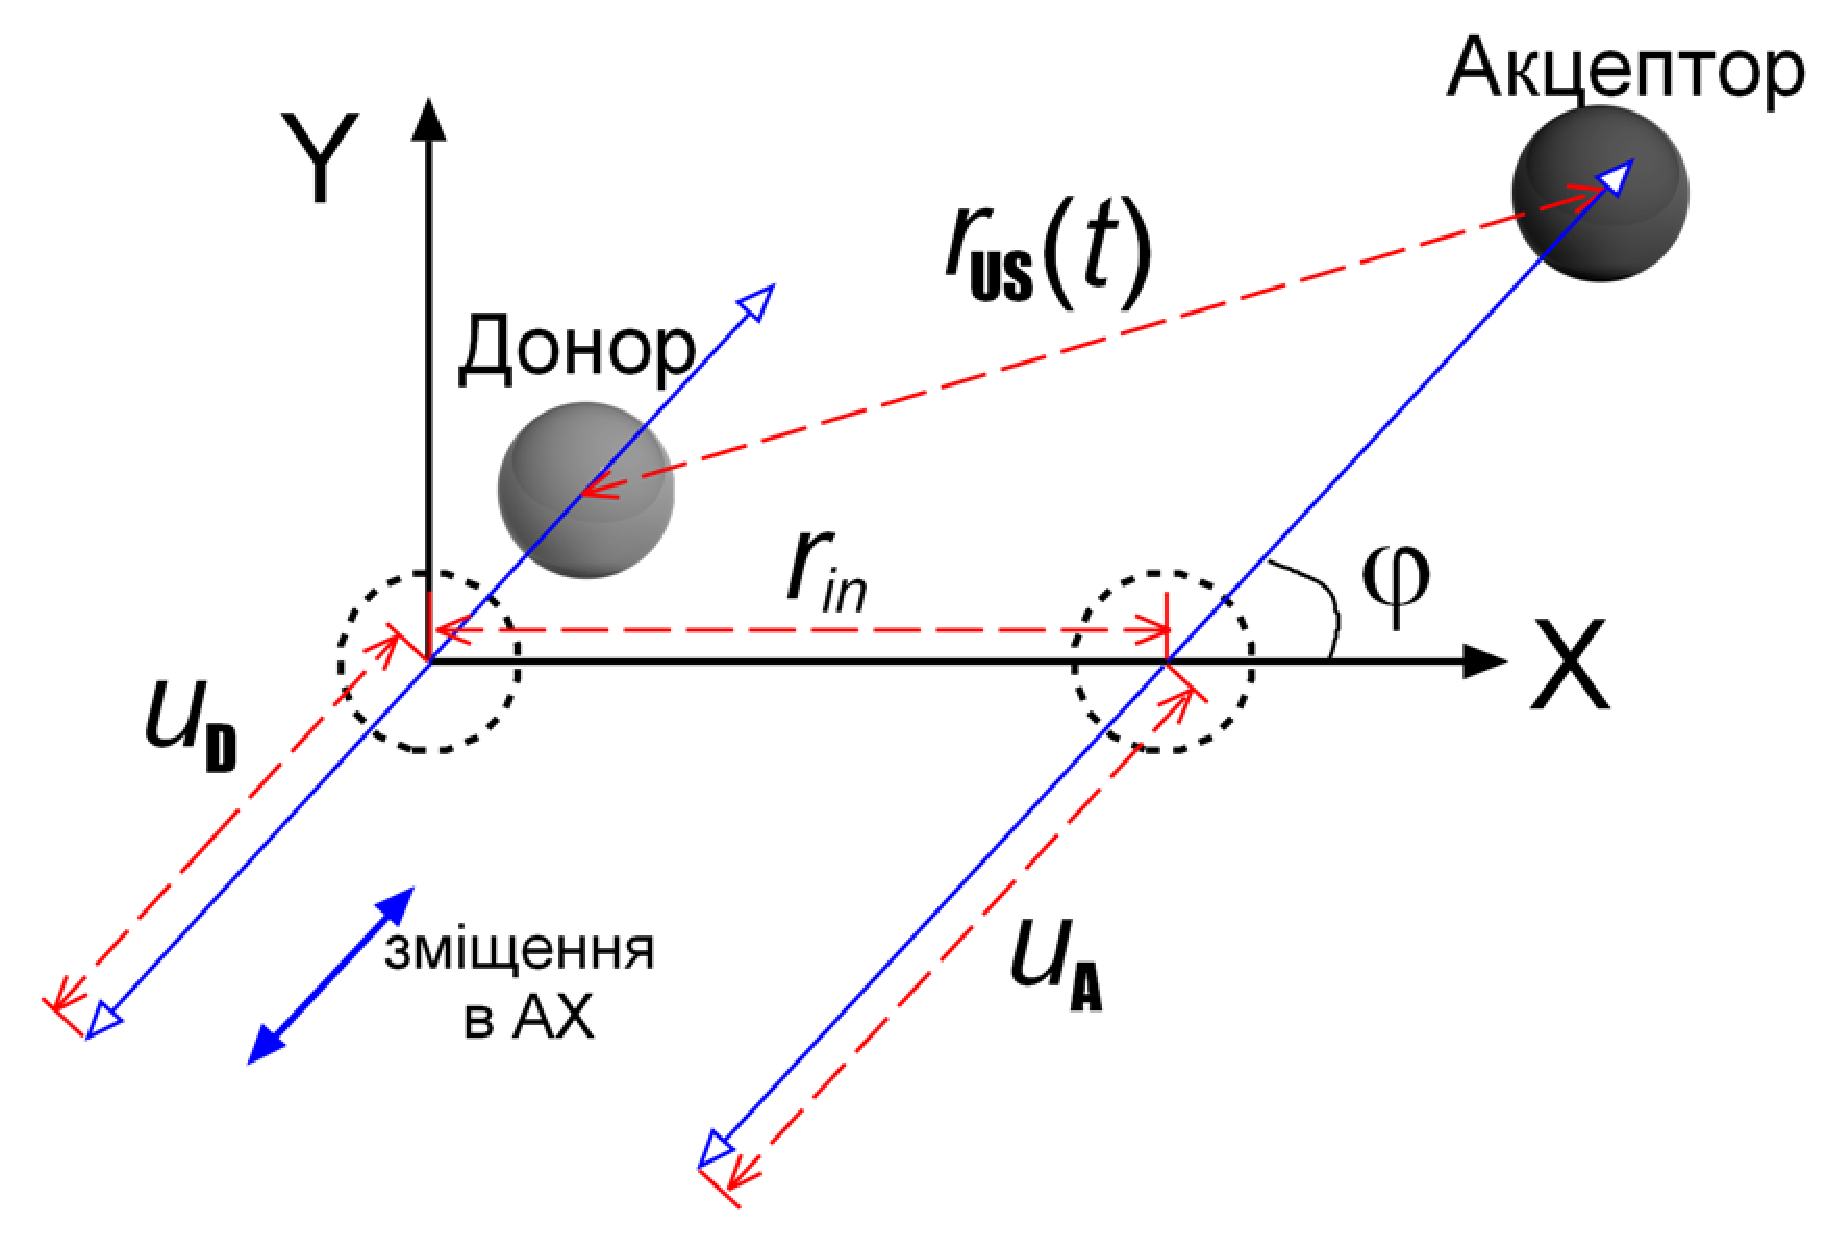
\includegraphics[width=0.5\textwidth]{fig_Model}
\caption{\label{fig_Model}
Модель поведінки дефектного комплексу в умовах УЗН
}%
\end{figure}

\begin{multline}
\label{eqrUS}
r_\mathtt{US}(t)=\left\{[r_{in}+u_\mathtt{A}\cos(2\pi f_\mathtt{US}t+\delta)-u_\mathtt{D}\cos(2\pi f_\mathtt{US}t)]^2\cos^2\varphi \right.\\
    \left.+ [u_\mathtt{A}\cos(2\pi f_\mathtt{US}t+\delta)-u_\mathtt{D}\cos(2\pi f_\mathtt{US}t)]^2\sin^2\varphi\right\}^{0.5}\,,
\end{multline}
де
$r_{in}$ --- вихідна відстань,
$u_\mathtt{D}$ та $u_\mathtt{A}$ --- амплітуди коливань компонент, $u_\mathtt{D},\,u_\mathtt{A}\sim u_\mathtt{US}$,
%$\omega_\mathtt{US}$ --- циклічна частота УЗ,
$\delta$ --- зсув фаз між коливаннями компонент,
$\varphi$ --- кут між віссю комплексу та напрямом зміщень в АХ.
В рамках запропонованої моделі були проведені розрахунки АІ змін $\sigma_{n}$ та так званого параметра зв'язку,
які визначають темп рекомбінації в наближеннях SRH та  CDLR.
Зокрема,
а)~визначено відмінності ефективності УЗ впливу для різних РЦ при збудженні поперечних та повздовжніх АХ з врахуванням наявності просторово орієнтованих дислокацій та показано, що найбільші АІ зміни очікуються у випадку, коли комплекс складається з компонент міжвузольного та вакансійного типу $(\Delta\Omega_d^\mathtt{D}\cdot\Delta\Omega_d^\mathtt{A}<0)$
 в умовах поперечних коливань;
б)~збільшення $\sigma_{n}$ та зменшення параметра зв'язку має викликати зменшення $\tau_g$ та зростання $n_\mathrm{id}$, що спостерігається на експерименті;
в)~для часу життя в КНО за умов УЗН $\tau_{n,\mathtt{US}}$ справедливе співвідношення
\begin{equation}
\label{eqEpsSigUSA}
\tau_{n,\mathtt{US}}^{-1}=
\tau_{n,in}^{-1}+u_{\mathtt{US}}^2\,\sum_j\,N_{d,j}\,\sigma_{n,j}^{in}\,K_\mathtt{US,j}\,\upsilon_{\mathrm{th},n}\,,
\end{equation}
де
сумування здійснюється лише по акустоактивних (АА) РЦ,
$K_\mathtt{US,j}$ описує взаємодію УЗ з дефектом $j$--го типу.

Виявлено зменшення величини шунтуючого опору (до 30\%) при УЗН.
Спираючись на температурну залежність $R_{sh}$ показано, що його поява може бути описана в рамках моделі дислокаційно--індукованого імпедансу
%\cite{Rsh:Gopal2004}
[3$^*$], а АІ зміни викликані зростанням ефективності захоплення електронів лінійними дефектами, розташованими в області $p$--$n$ переходу.

Проведені в рамках дводіодної моделі чисельні розрахунки показали, що АІ зміни $J_{sc}$ пов'язані зі зменшенням $\tau_{n}$,
тоді як зменшення $\tau_{g}$ викликає деградацію як $V_{oc}$, так i $F\!F$.
Ефект деградації підсилюється внаслідок АI зменшення $R_{sh}$ та частково компенсується зростанням $n_\mathrm{id}$.

Додатково, за допомогою методу диференційним коефіцієнтів ВАХ
%\cite{Bulyar}
[4$^*$], визначено вплив УЗН на параметри дефектів, розташованих в ОПЗ неопромінених КСЕ.
Шляхом детального аналізу літературних даних проведена ідентифікація дефектів, пов'язаних з виявленими енергетичними рівнями.
А саме, основними дефектами є КП (рівні $E_c-(0,46\div0,48)$~еВ та $E_c-0,40$~еВ), дислокації ($E_c-0,36$~еВ) та комплекси Fe$_i$O$_i$ ($E_c-0,43$~еВ).
При УЗН відбувається незначне (близько 0,01~еВ) зменшення енергії активації та збільшується внесок
у рекомбінацію більш мілких рівнів, зокрема КП, причому зміни відносних внесків різних центрів практично лінійно залежать від $u_\mathtt{US}$.

Також представлені результати аналізу ВАХ, виміряних за умов УЗН та без нього, для КСЕ опромінених $\gamma$--квантами $^{60}$Co (доза $D$ $10^6$ та $10^7$~рад) та реакторними нейтронами (флюєнс $4\cdot10^{11}$~см$^{-2}$).
Використовуючи літературні дані показано, що при нейтронному опроміненні виникають К--центри (пара C$_i$O$_i$ ),
вакансійні кластери V$_n$ та А--центри (пара VO$_i$), тоді як $\gamma$--промені мають викликати появу лише, переважно, C$_i$O$_i$ та VO$_i$;
проведено оцінку концентрацій радіаційних дефектів та їх впливу на $\tau_n$.

\begin{figure}[ht]
\center
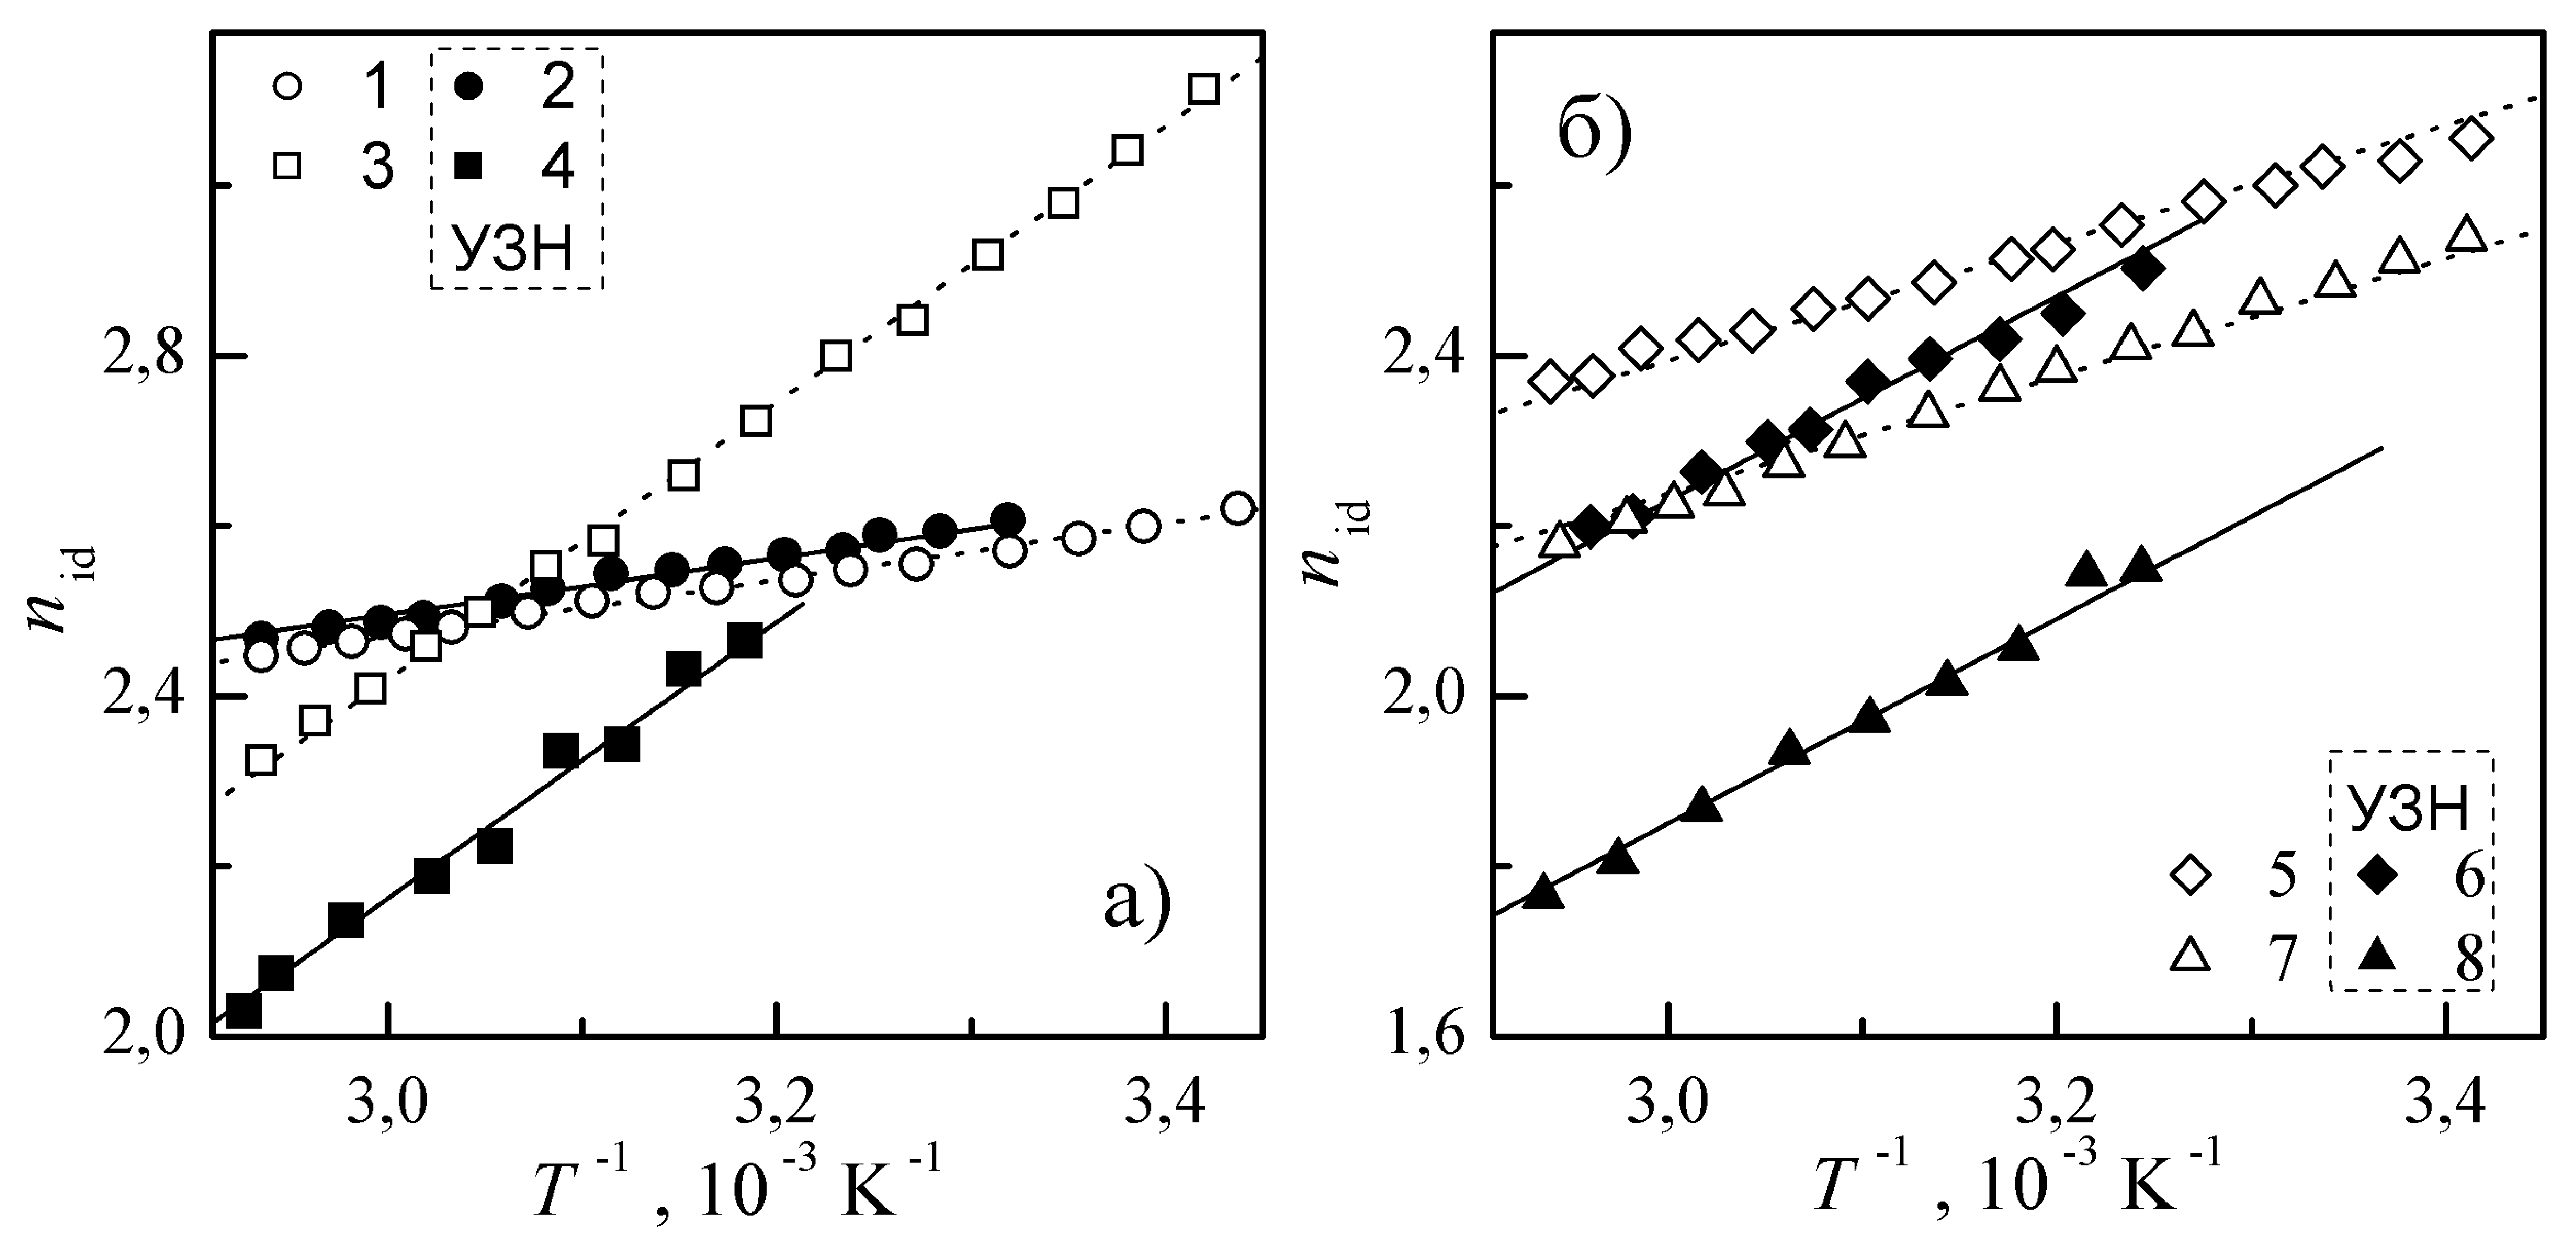
\includegraphics[width=0.9\textwidth]{fignRD}%
\caption{\label{fignRD}
Температурні залежності фактора неідеальності
для неопроміненого (криві 1, 2),
нейтронно--опроміненого (3, 4) та
$\gamma$--опромінених (5, 6 та 7, 8 для доз $10^6$ та $10^7$~рад, відповідно)
зразків.
Криві 1, 3, 5 та 6 отримані без УЗН,
криві 2, 4, 9 та 8 відповідають УЗН (поперечні хвилі, 4,2~МГц, 0,4~Вт/см$^2$)
}%
\end{figure}


\begin{figure}[ht]
\center
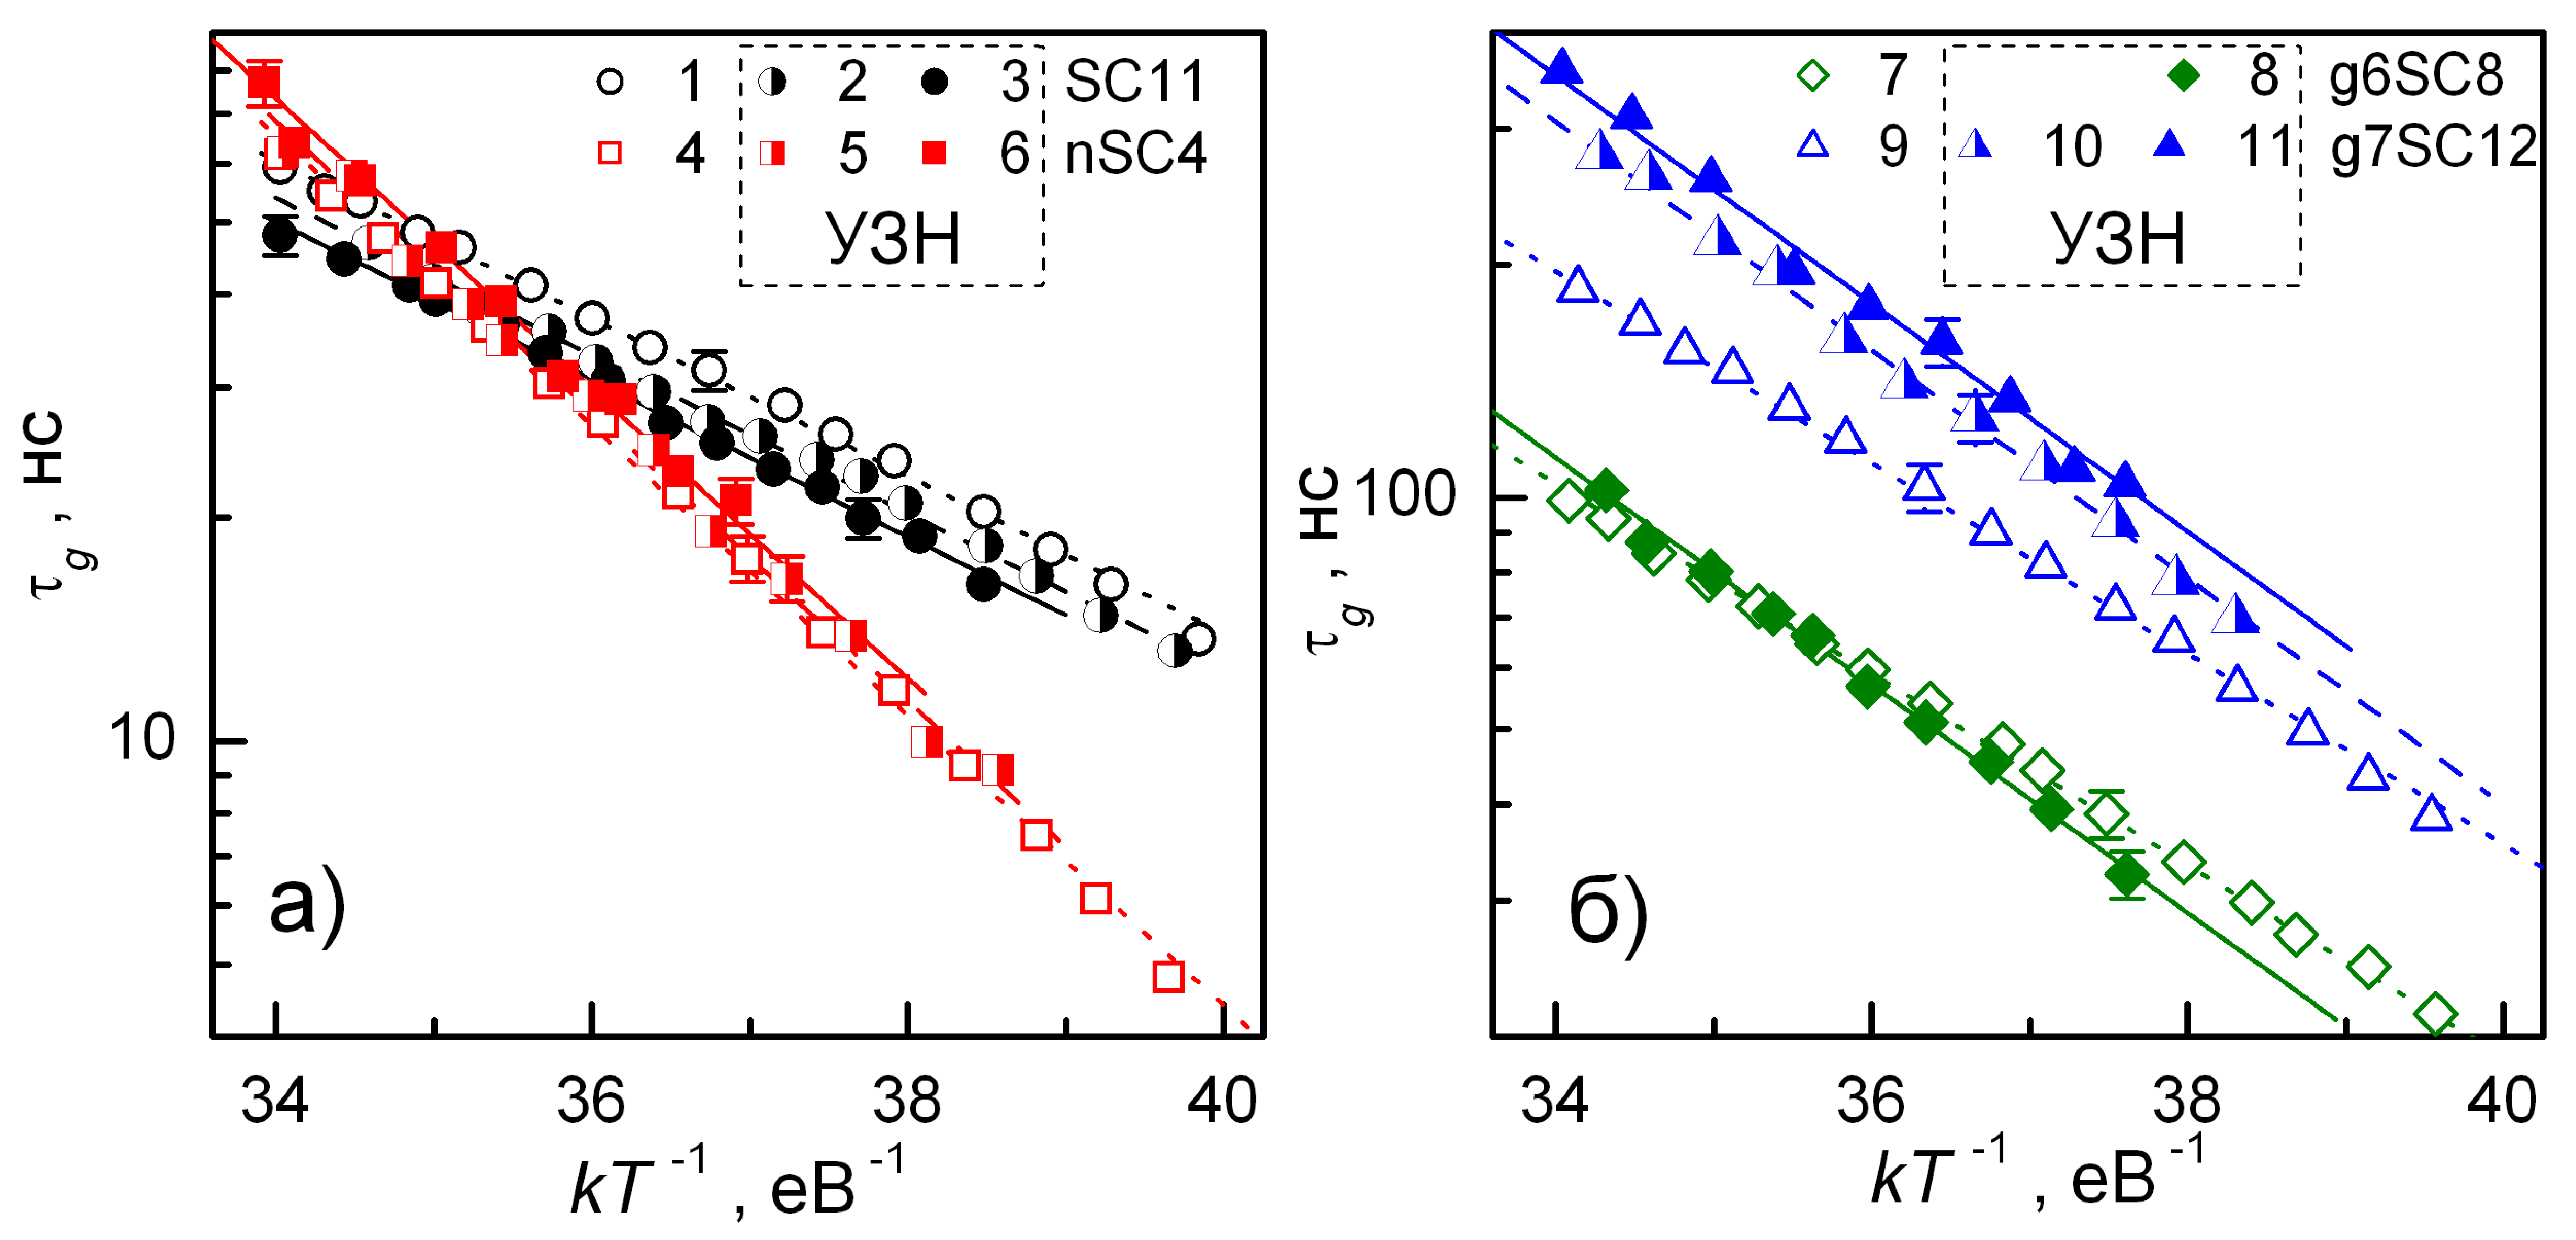
\includegraphics[width=0.9\textwidth]{figTAUgRD}%
\caption{\label{figTAUgRD}
Температурні залежності $\tau_g$.
Позначення кривих збігаються з рис.~\ref{fignRD}
}%
\end{figure}

При розгляді параметрів, що характеризують рекомбінаційні процеси в ОПЗ виявлено, що
а)~характер температурних залежностей  $\tau_{g}$ та $n_\mathrm{id}$ співпадає з неопроміненими структурами (рис.~\ref{fignRD} та \ref{figTAUgRD}), проте величини $T_{\mathrm{id}}$ та $E_{\tau g}$ інші, а отже
в опромінених КСЕ в  процесах CDLR приймає участь, що найменше, один інший дефект порівняно з неопроміненими;
б)~АІ зміни $n_\mathrm{id}$ в радіаційно модифікованих структурах більші за величиною та протилежні за знаком до АІ змін у вихідних КСЕ;
в рамках моделі акустоактивного комплексного РЦ це свідчить про те, що до опромінення $\Delta\Omega_d^\mathtt{D}\cdot\Delta\Omega_d^\mathtt{A}>0$, а після $\Delta\Omega_d^\mathtt{D}\cdot\Delta\Omega_d^\mathtt{A}<0$;
в)~за умов УЗН величини $T_{\mathrm{id}}$ та $E_{\tau g}$ в $\gamma$--опромінених структурах оборотно змінюються,
тоді як для неопромінених та нейтронно--опромінених КСЕ співпадають зі значеннями, отриманими за відсутності АХ;
подібна поведінка засвідчує, що в $\gamma$--опромінених зразках відбувається акустоіндукована перебудова метастабільного дефекту, яким, найшвидше, є А--центр;
В нейтронно--опромінених структурах центром, який відповідає за АІ зміни $\tau_{g}$ та $n_\mathrm{id}$, є дивакансія.

Показано, що при УЗН величина $\tau_n^{-1}$ і для опромінених структур лінійно залежала від $u_{\mathtt{US}}^2$.
Використовуючи співвідношення~(\ref{eqEpsSigUSA}) та оцінені концентрації радіаційних дефектів, отримана система рівнянь для визначення коефіцієнтів, які характеризують акусто--дефектну взаємодію радіаційних дефектів та КП.
Її розв'язок показав, що для К--центру $K_\mathtt{US}^\mathtt{CO}=0$, тобто цей дефект не є акустоактивним,
для дивакансії $K_\mathtt{US}=(42\pm15)$~см$^2$~Вт$^{-1}$, для КП $K_\mathtt{US}>5$~см$^2$~Вт$^{-1}$.

\begin{figure}[ht]
\center
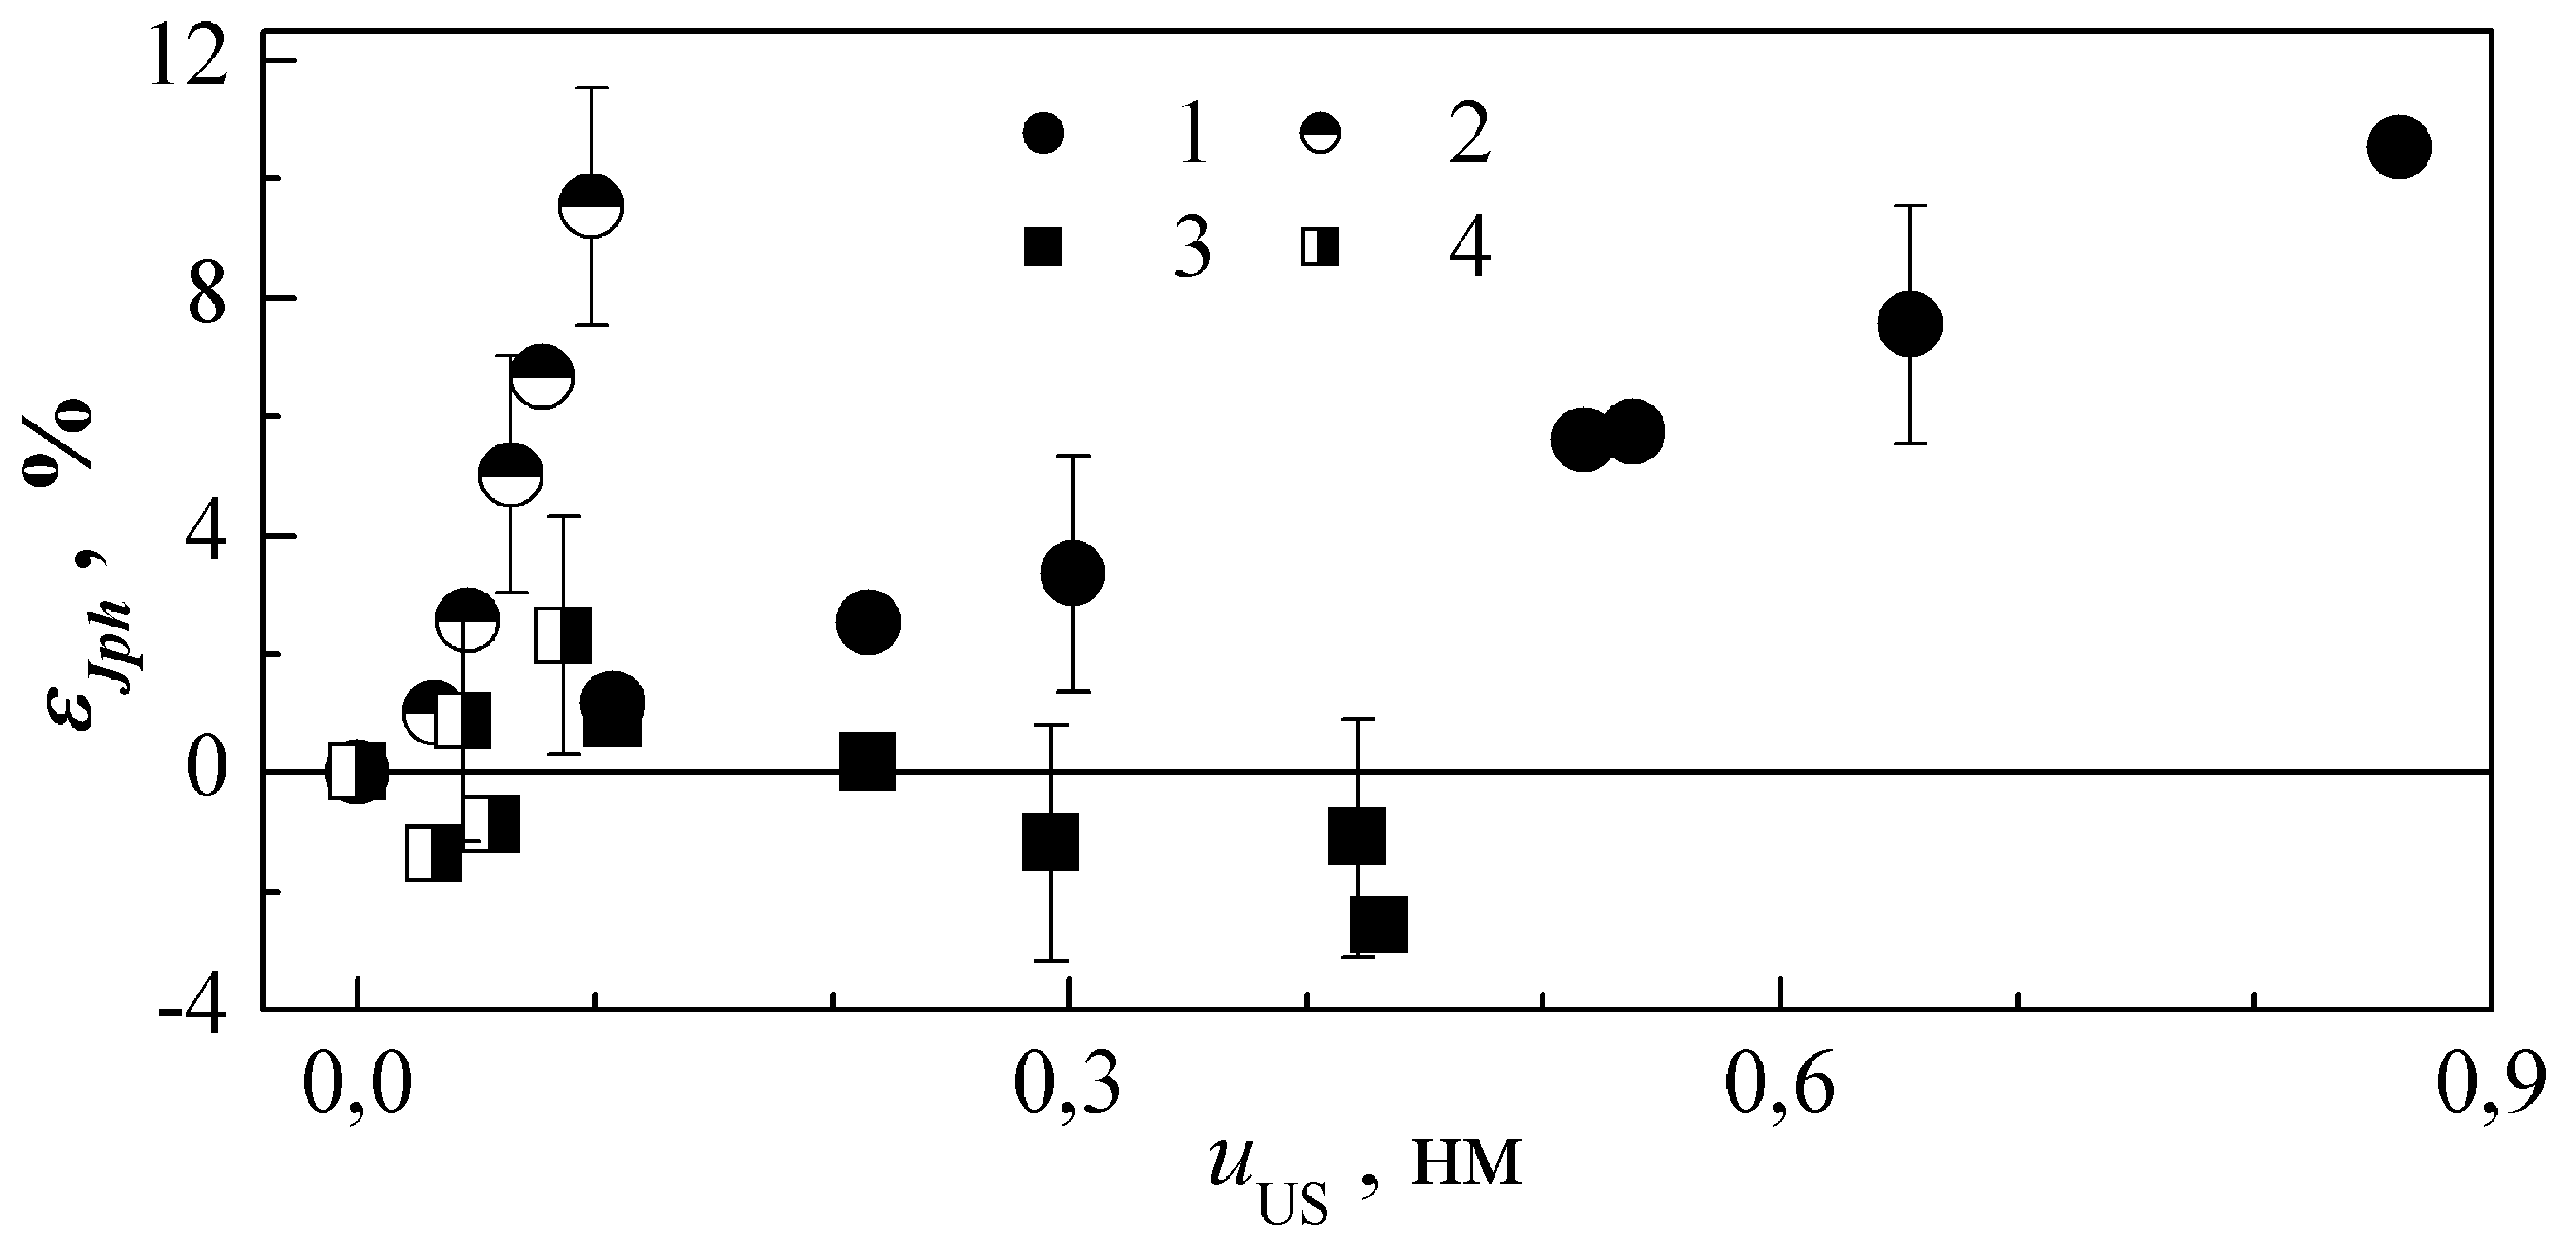
\includegraphics[width=0.6\textwidth]{figeIscRD}
\caption{\label{figeIscRD}
Залежності АІ зменшення фотоструму від
амплітуди зміщень атомів в неопроміненому (1, 2)
та нейтронно--опроміненому (3, 4) зразках.
$f_\mathtt{US}$, Гц: 8,0 (1, 3);
26,1 (2, 4)
}%
\end{figure}
Повідомляється також про результати дослідження фотоелектричного перетворення в опромінених КСЕ.
Виявлено, що УЗН $\gamma$--опромінених структур, як і неопромінених, викликає зменшення величини $J_{ph}$, що цілком
узгоджується з виявленим АІ підвищенням активності рекомбінаційних центрів (зменшенням $\tau_n$).
Водночас для нейтронно-опромінених зразків АІ змін $J_{ph}$ практично не спостерігається --- рис.~\ref{figeIscRD}.
Встановлено, що при нагріванні за відсутності УЗН і в неопромінених, і в нейтронно-опромінених КСЕ зміна фотоструму
цілком узгоджується зі змінами довжини дифузії неосновних носіїв заряду $L_n$ (для визначення якої використовувався метод SSSCC).
Водночас при нагріванні нейтронно-опромінених структур під час УЗН зміни $J_{ph}$ не можуть бути пояснені лише змінами $L_n$ на відміну від неопромінених КСЕ.
Виявлені особливості свідчать про наявність додаткового механізму впливу УЗН на процеси генерації струму у нейтронно--опромінених структурах;
на думку автора, причиною виявленого ефекту є АІ зміна заселеності рівнів, пов'язаних з вакансійними кластерами, що викликає зменшення коефіцієнта відбивання світла.


Наведені   результати  підтверджують  практичну перспективність динамічного акустичного керування характеристиками напівровідникових приладів.
Підкреслимо, що нерівноважний стан дефектів, який виникає при появі нерівноважних носіїв при проходженні струму, є важливим фактором підвищення ефективності акусто--дефектної взаємодії.

У  \underline{\textbf{третьому розділі}} представлені результати поріняльного аналізу та оптимізації методів розрахунку параметрів структур метал--напівпровідник (МН).
Увага була зосереджена на визначенні струму насичення  $I_s$ (висоти бар'єру Шотткі, (ВБШ) $\Phi_b$), фактора неідеальності та послідовного опору з ВАХ, яка, як відомо, при переважанні термоелектронної емісії (ТЕ), має описуватися виразом

\begin{eqnarray}
\label{eqSDIV}
\nonumber I&=&I_s\left\{\exp\left[\frac{q(V-IR_s)}{n_\mathrm{id}kT}\right]-1\right\}=\\
&=&AA^*\,T^2\exp\left(-\frac{q\Phi_b}{kT}\right)\left\{\exp\left[\frac{q(V-IR_s)}{n_\mathrm{id}kT}\right]-1\right\}\,,
\end{eqnarray}
де
$A$ --- площа діоду Шотткі,
$A^*$ --- ефективна стала Річардсона.
Були розглянуті 10 аналітичних методів (використовують інтегрування ВАХ (метод Kaminski І), побудову різноманітних допоміжних функцій (чи їх масиву) та лінійну (методи Chung, Lee та Kaminski ІІ) чи нелінійну (Gromov) апроксимацію або пошук екстремумів (Cibils);
іноді для побудови функцій застосовують додаткові параметри (методи Norde та Bohlin) або диференційні коефіцієнти першого (Werner) або вищого порядків (Mikhelashvili))
2 чисельних методи (метод найменших квадратів зі статичними ваговими коефіцієнтами застосовувався безпосередньо до рівняння~(\ref{eqSDIV}) та до його розв'язку, вираженого через $W$--функцію Ламберта) та
4 еволюційних алгоритми (диференційної еволюції (DE),
оптимізації зграї частинок (PSO),
модифікованої штучної бджолиної сім'ї (MABC) та
оптимізованого викладання та навчання (TLBO)).
Всі методи були застосовані до
а)~синтезованих за допомогою виразу~(\ref{eqSDIV}) ідеальних ВАХ;
б)~синтезованих ВАХ з врахуванням можливих випадкових похибок вимірювань;
в)~експериментально виміряних ВАХ кремнієвих діодів Шотткі.

Для методів Norde та Bohlin визначені  оптимальні (для кремнієвих діодів Шотткі при вимірюваннях в діапазоні температур $130\div330$~К) величини додаткових параметрів (1,8 для Norde та 1,6 і 3,5 для Bohlin).
Запропоновано модифікацію методу Mikhelashvili, яка дозволяє застосовувати його в автоматичному режимі до множини ВАХ;
вона полягає у послідовному використанні медіанного фільтру та процедури згладжування функції $\alpha(V)=d(\ln I)/d(\ln V)$ перед визначенням положення її максимуму.
Показано доцільність застосування запропонованої процедури при опрацюванні реальних ВАХ для підвищення точності методу.
Запропоновано адаптивну процедуру вибору діапазону ВАХ, який використовується для побудови допоміжних функцій при застосуванні аналітичних методів визначення параметрів структур МН та показано, що вона дозволяє підвищити точність визначення параметрів (приблизно на порядок при кімнатних температурах у випадку низького рівня похибок вимірювання) і не викликає критичного збільшення часу розрахунку.

\begin{table}[b]
\caption{\label{tabRT}Час визначення параметрів ДШ з однієї ВАХ}
\centering
\begin{tabular}{|r|c|r|c|}
\hline
\multicolumn{1}{|c|}{Метод}&Час роботи, с &\multicolumn{1}{c|}{Метод}&Час роботи, с\\ \hhline{|====|}
Norde &$(2,6\div3,7)\cdot10^{-5}$& Werner  &$(4,0\div4,5)\cdot10^{-5}$\\ \hline
Cibils  &$(0,2\div5,3)\cdot10^{-3}$& Kaminskii I &$(4,5\div8,0)\cdot10^{-5}$\\ \hline
Kaminskii II &$(0,3\div2,6)\cdot10^{-3}$& Bohlin &$(4,0\div6,3)\cdot10^{-5}$\\ \hline
Lee &$(0,2\div3,6)\cdot10^{-3}$& Gromov &$2.2\cdot10^{-2}$\\ \hline
Cheung &$(2,0\div3,2)\cdot10^{-5}$&Mikhelashvili &$(2,9\div4,7)\cdot10^{-5}$\\ \hline
Ordinary LS &$1,8\div460$&Lambert LS &$7,6\div540$\\ \hline
DE &$0,36\div0,73$&PSO &$0,14\div0,35$\\ \hline
MABC &$5.7\cdot10^{-2}\div0,20$&TLBO &$5.4\div19,2$ \\
\hline
\end{tabular}
\end{table}

Основна задача полягала у порівнянні точності (рис.~\ref{figId} та \ref{figPrAcc}) та швидкодії (табл.~\ref{tabRT}) визначення параметрів структур МН різними методами.
Показано, що найбільша точність досягається при використанні еволюцiйних алгоритмів (ЕА), чисельних методів, метод Gromov з адаптивною процедурою та метод Lee.
Використання функції Ламберта при застосуванні чисельних методів дозволяє зменшити помилки визначення параметрів.
Визначено вплив абсолютних величин кожного з параметрів на точність визначення $R_s$, $\Phi_b$ та $n_\mathrm{id}$.
Зокрема показано, що ЕА дозволяють отримати найбільш коректні результати при малих (декілька Ом) значеннях $R_s$ або високих температурах, а найбільш стійкими до величин параметрів є точності чисельних методів.


\begin{figure}
\center
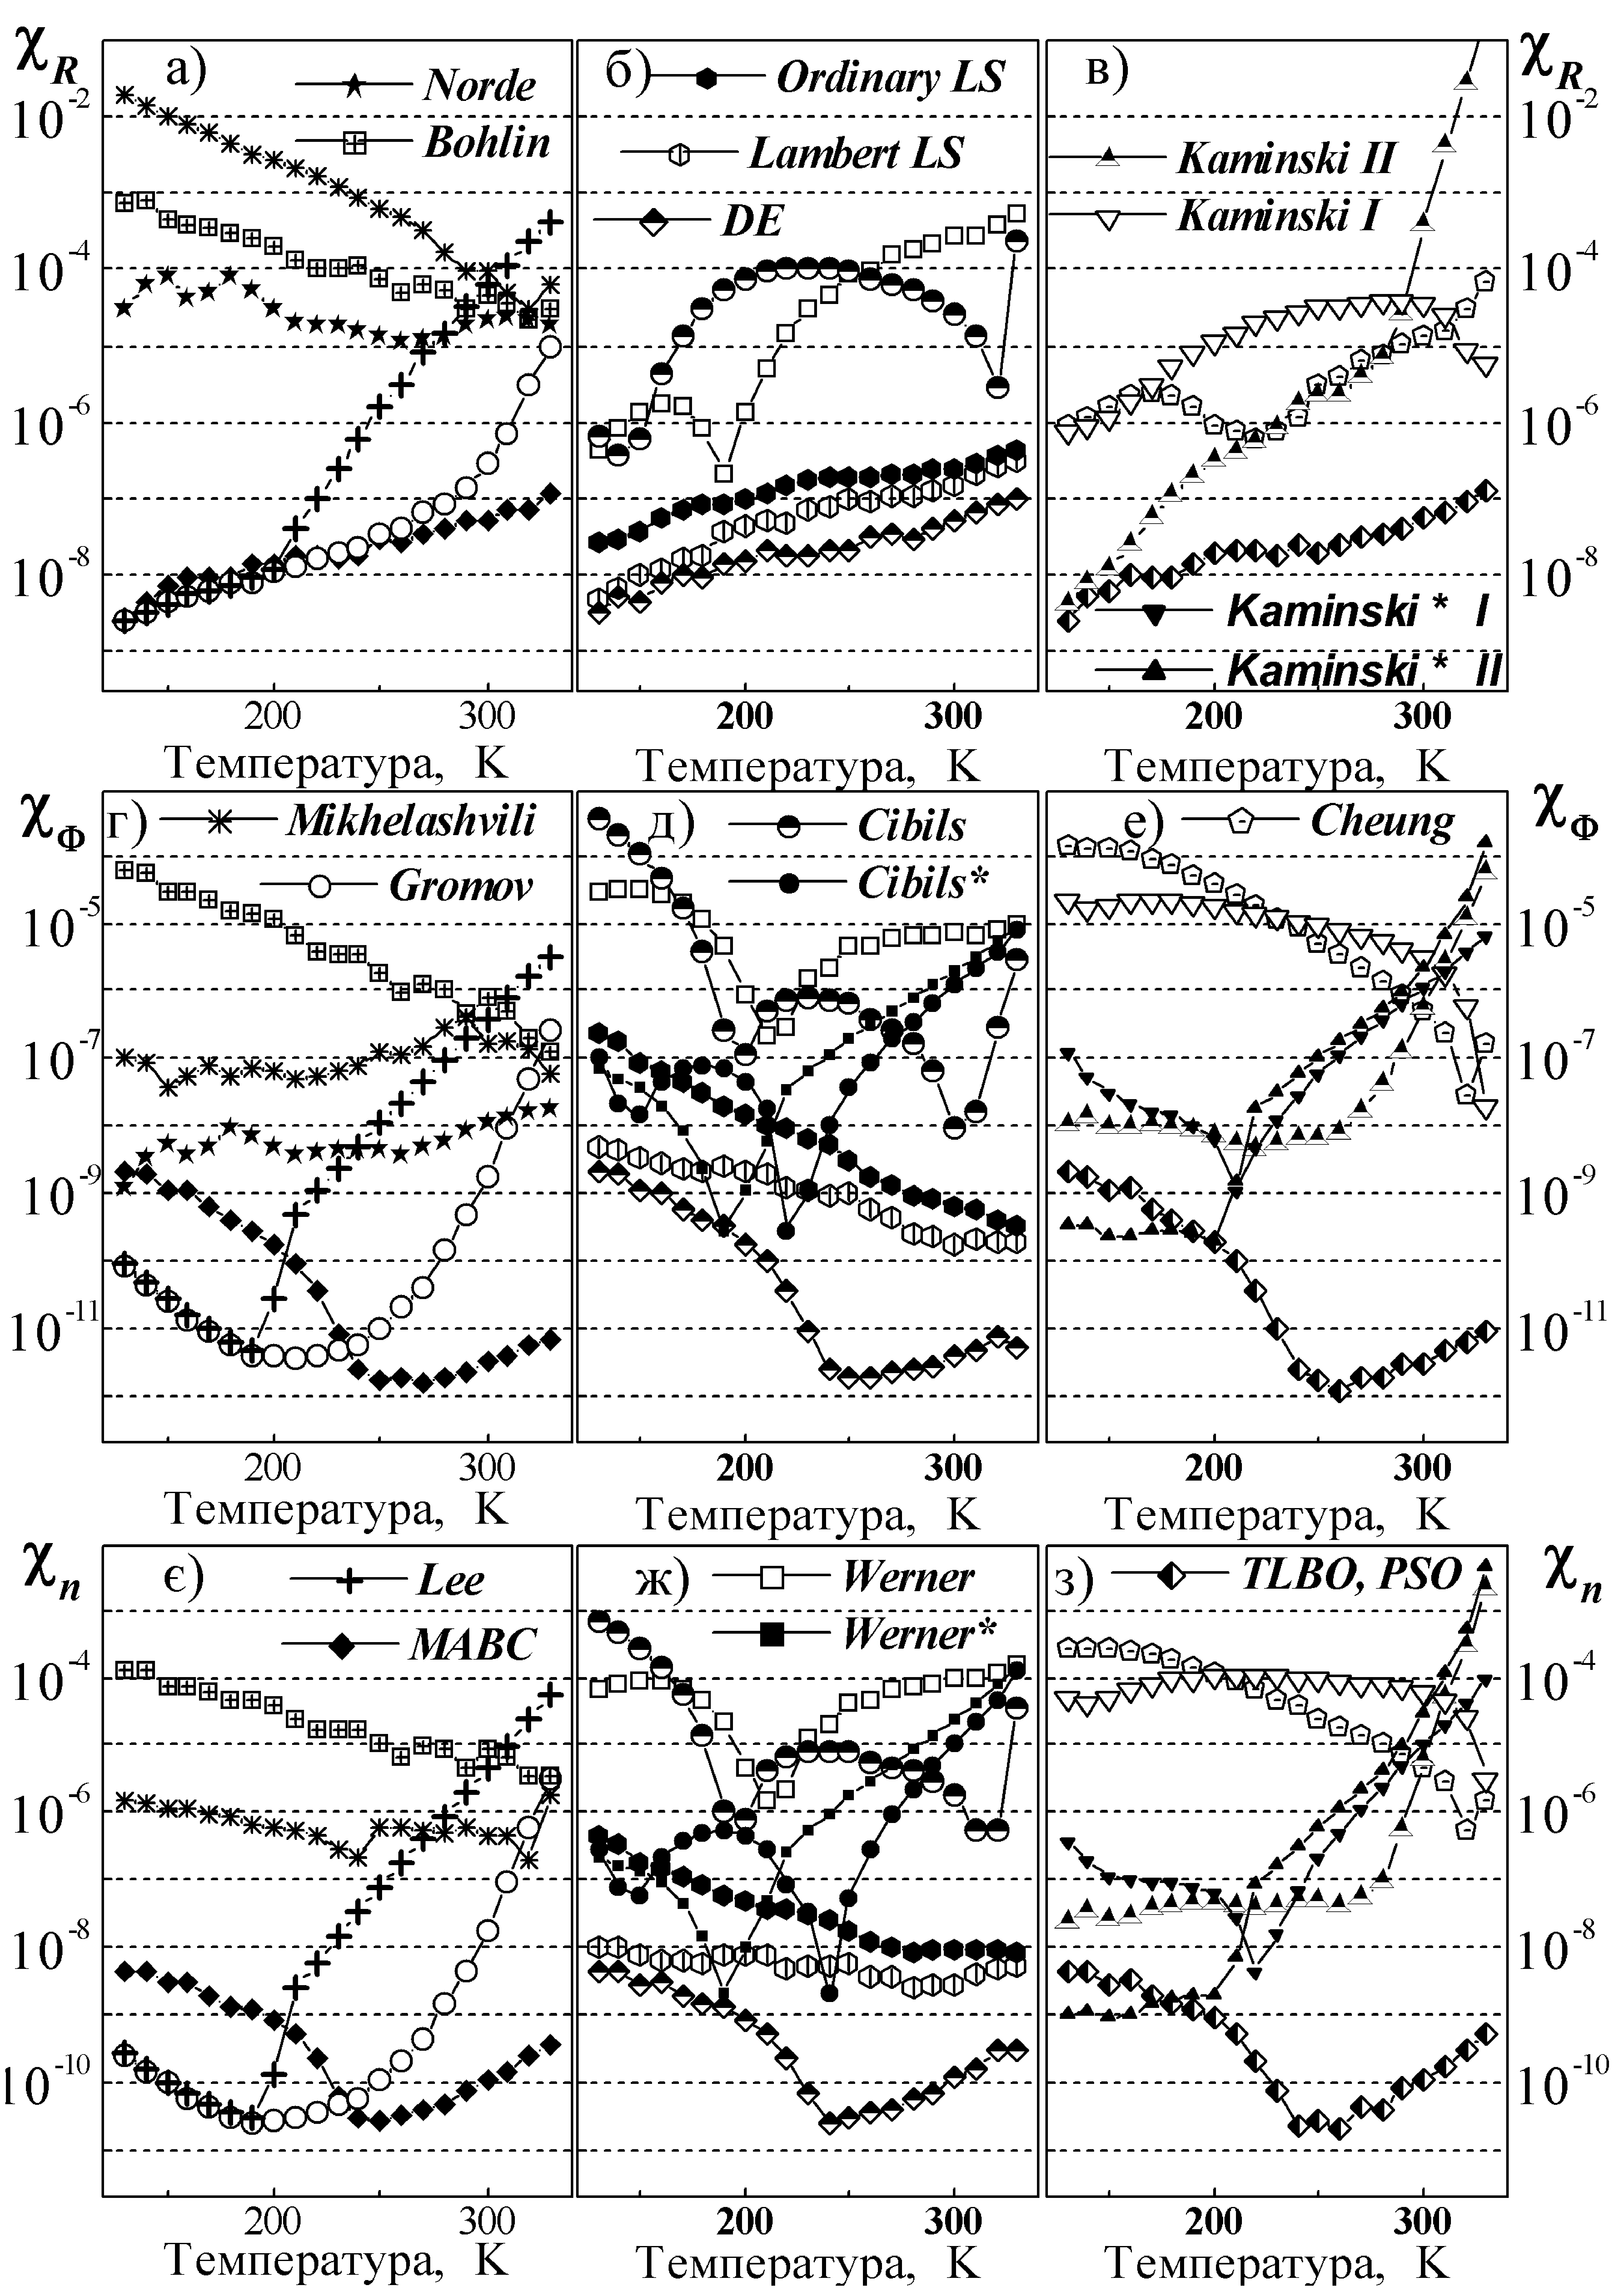
\includegraphics[width=0.75\textwidth]{figId}%
\caption{\label{figId}
Температурні залежності відносних похибок визначення $R_s$ (а --- в), $\Phi_b$ (г --- е) та $n_\mathrm{id}$ (є --- з) при застосуванні методів до ідеальних синтезованих ВАХ
}
\end{figure}

\begin{figure}
\center
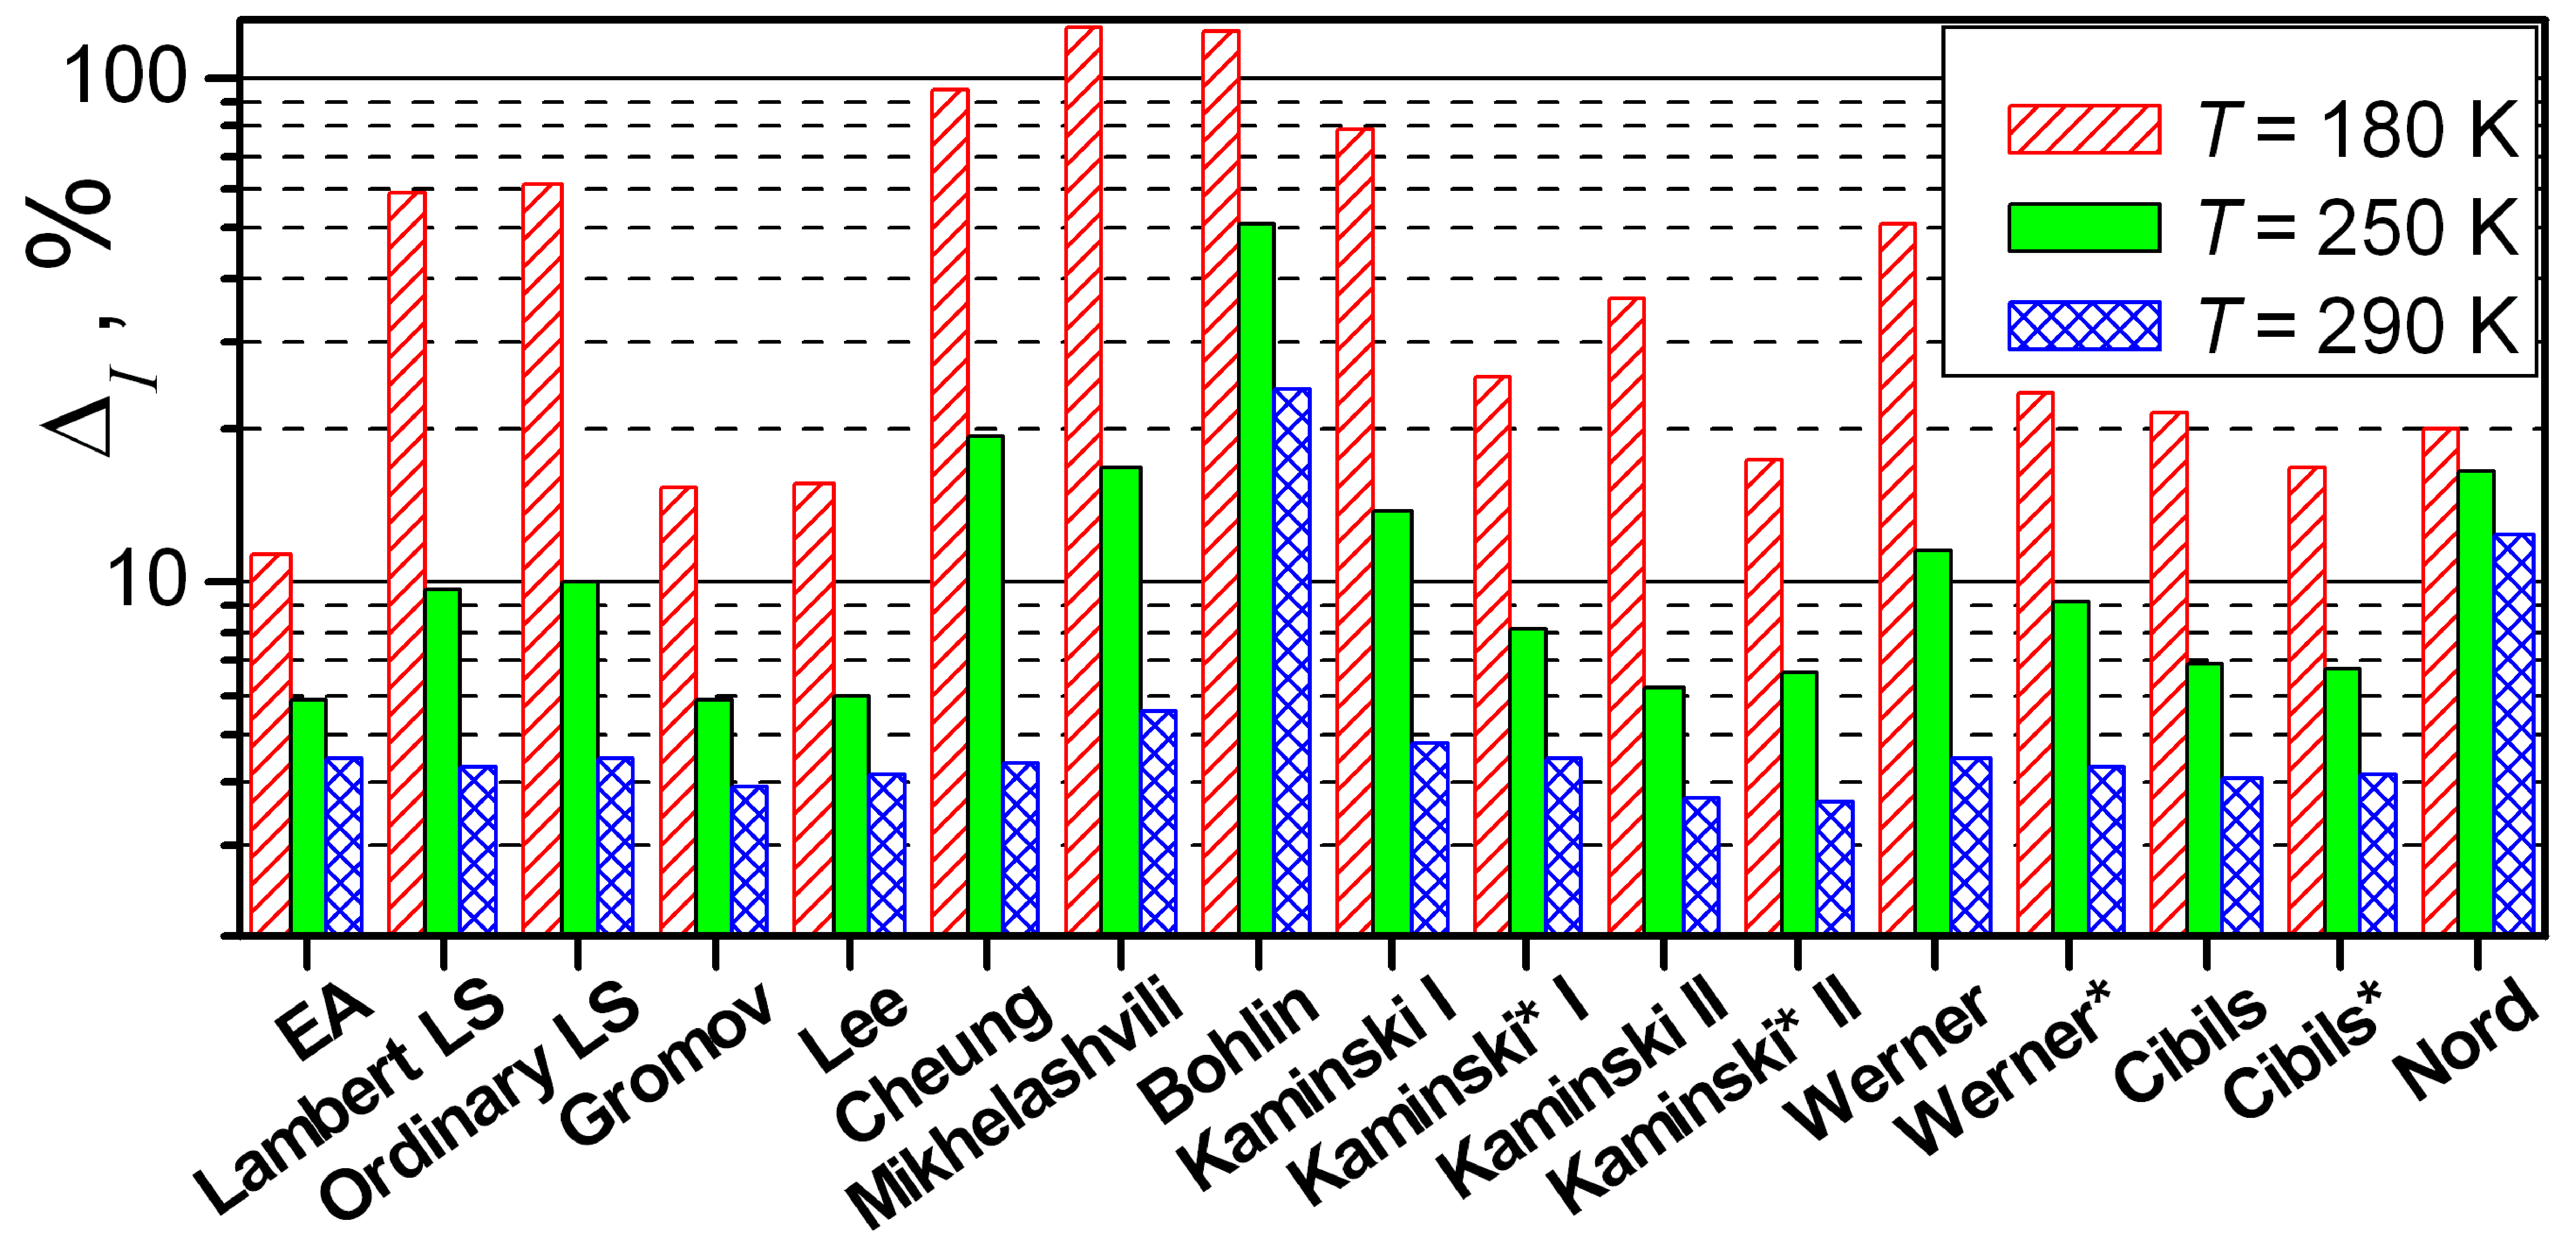
\includegraphics[width=0.8\textwidth]{figPrAcc}%
\caption{\label{figPrAcc}
Середні значення відносного відхилення розрахованих значень сили струму від експериментальних даних
}
\end{figure}


Аналіз залежності точності визначення параметрів від випадкових похибок вимірювань показав, що практично для всіх методів
а)~відносні похибки визначення $R_s$, $\Phi_b$ та $n_\mathrm{id}$ лінійно залежать як від величин відносних похибок вимірювання напруги, так і сили струму, причому в останньому випадку залежність слабша;
б)~помилки визначення $\Phi_b$ та $n_\mathrm{id}$ значно менші, ніж помилки визначення $R_s$ за тих самих умов вимірювання.

Важливо підкреслити, що представлені результати огляду, тестування та порівняльного аналізу методів визначення параметрів діодів Шотткі можуть бути корисними під час досліджень та розробок пристроїв з контактом МН на базі не лише кремнію, але й інших напівпровідників.


У  \underline{\textbf{четвертому розділі}} представлені результати досліджень
номонотонного впливу $\gamma$--опромінення на структури Al$-n-n^+$--Si---Al з контактом Шотткі та
динамічних АІ ефектів при кімнатних температурах.
Основними завданнями, які вирішувались під час цих досліджень, полягали у з'ясуванні механізмів перенесення заряду при прямому та
    зворотному зміщеннях в широкому діапазоні температур ($130\div330$~K) та шляхів модифікації внаслідок $\gamma$--опромінення, а також вивчення вперше виявлених
    оборотних АІ ефектів в МН структурах.

Виявлено, що для неопромінених структур спостерігається поява при низьких ($T<210$~К) температурах додаткової компоненти струму,
збільшення ВБШ при зростанні температури (рис.~\ref{figFbTrad_SDA}) та зменшення фактора неідеальності:
\begin{equation}\label{eqN_T:TE}
n_{\mathrm{id}}=1+\frac{T_0}{T},
\end{equation}
де $T_0=12$~K.
Показано, що всі виявлені особливості можна пояснити з точки зору моделі ТЕ через неоднорідний контакт
%\cite{Tung:MSE}
[5$^*$].
Про це свідчать лінійність залежностей $\Phi_{b}$ та $(n_{\mathrm{id}}^{-1}-1)$ від $q/2kT$, $\Phi_{b}$ від $n_{\mathrm{id}}$,
збіг експериментально визначеного значення $T_0$  та відомого з літератури значення $A^*$ (112~А$\cdot$см$^{-2}\cdot$К$^{-2}$) з відповідними величинами,
розрахованими в рамках цієї моделі на основі температурної залежності ВБШ.
       Визначені середня висота бар'єру Шотткі $\Phi_b^0$ та її стандартне відхилення $\sigma_{\Phi}$:
       $0,872\pm0,004$~В та $0,099\pm0,001$~В при $(130\div220)$~К та
       $0,663\pm0,003$~В та $0,040\pm0,005$~В при $(230\div330)$~К, відповідно.
Визначено середнє значення висоти бар'єру Шотткі в області зі зниженим бар'єром (в області патчу) $54\pm4$~мВ.

\begin{figure}
\center
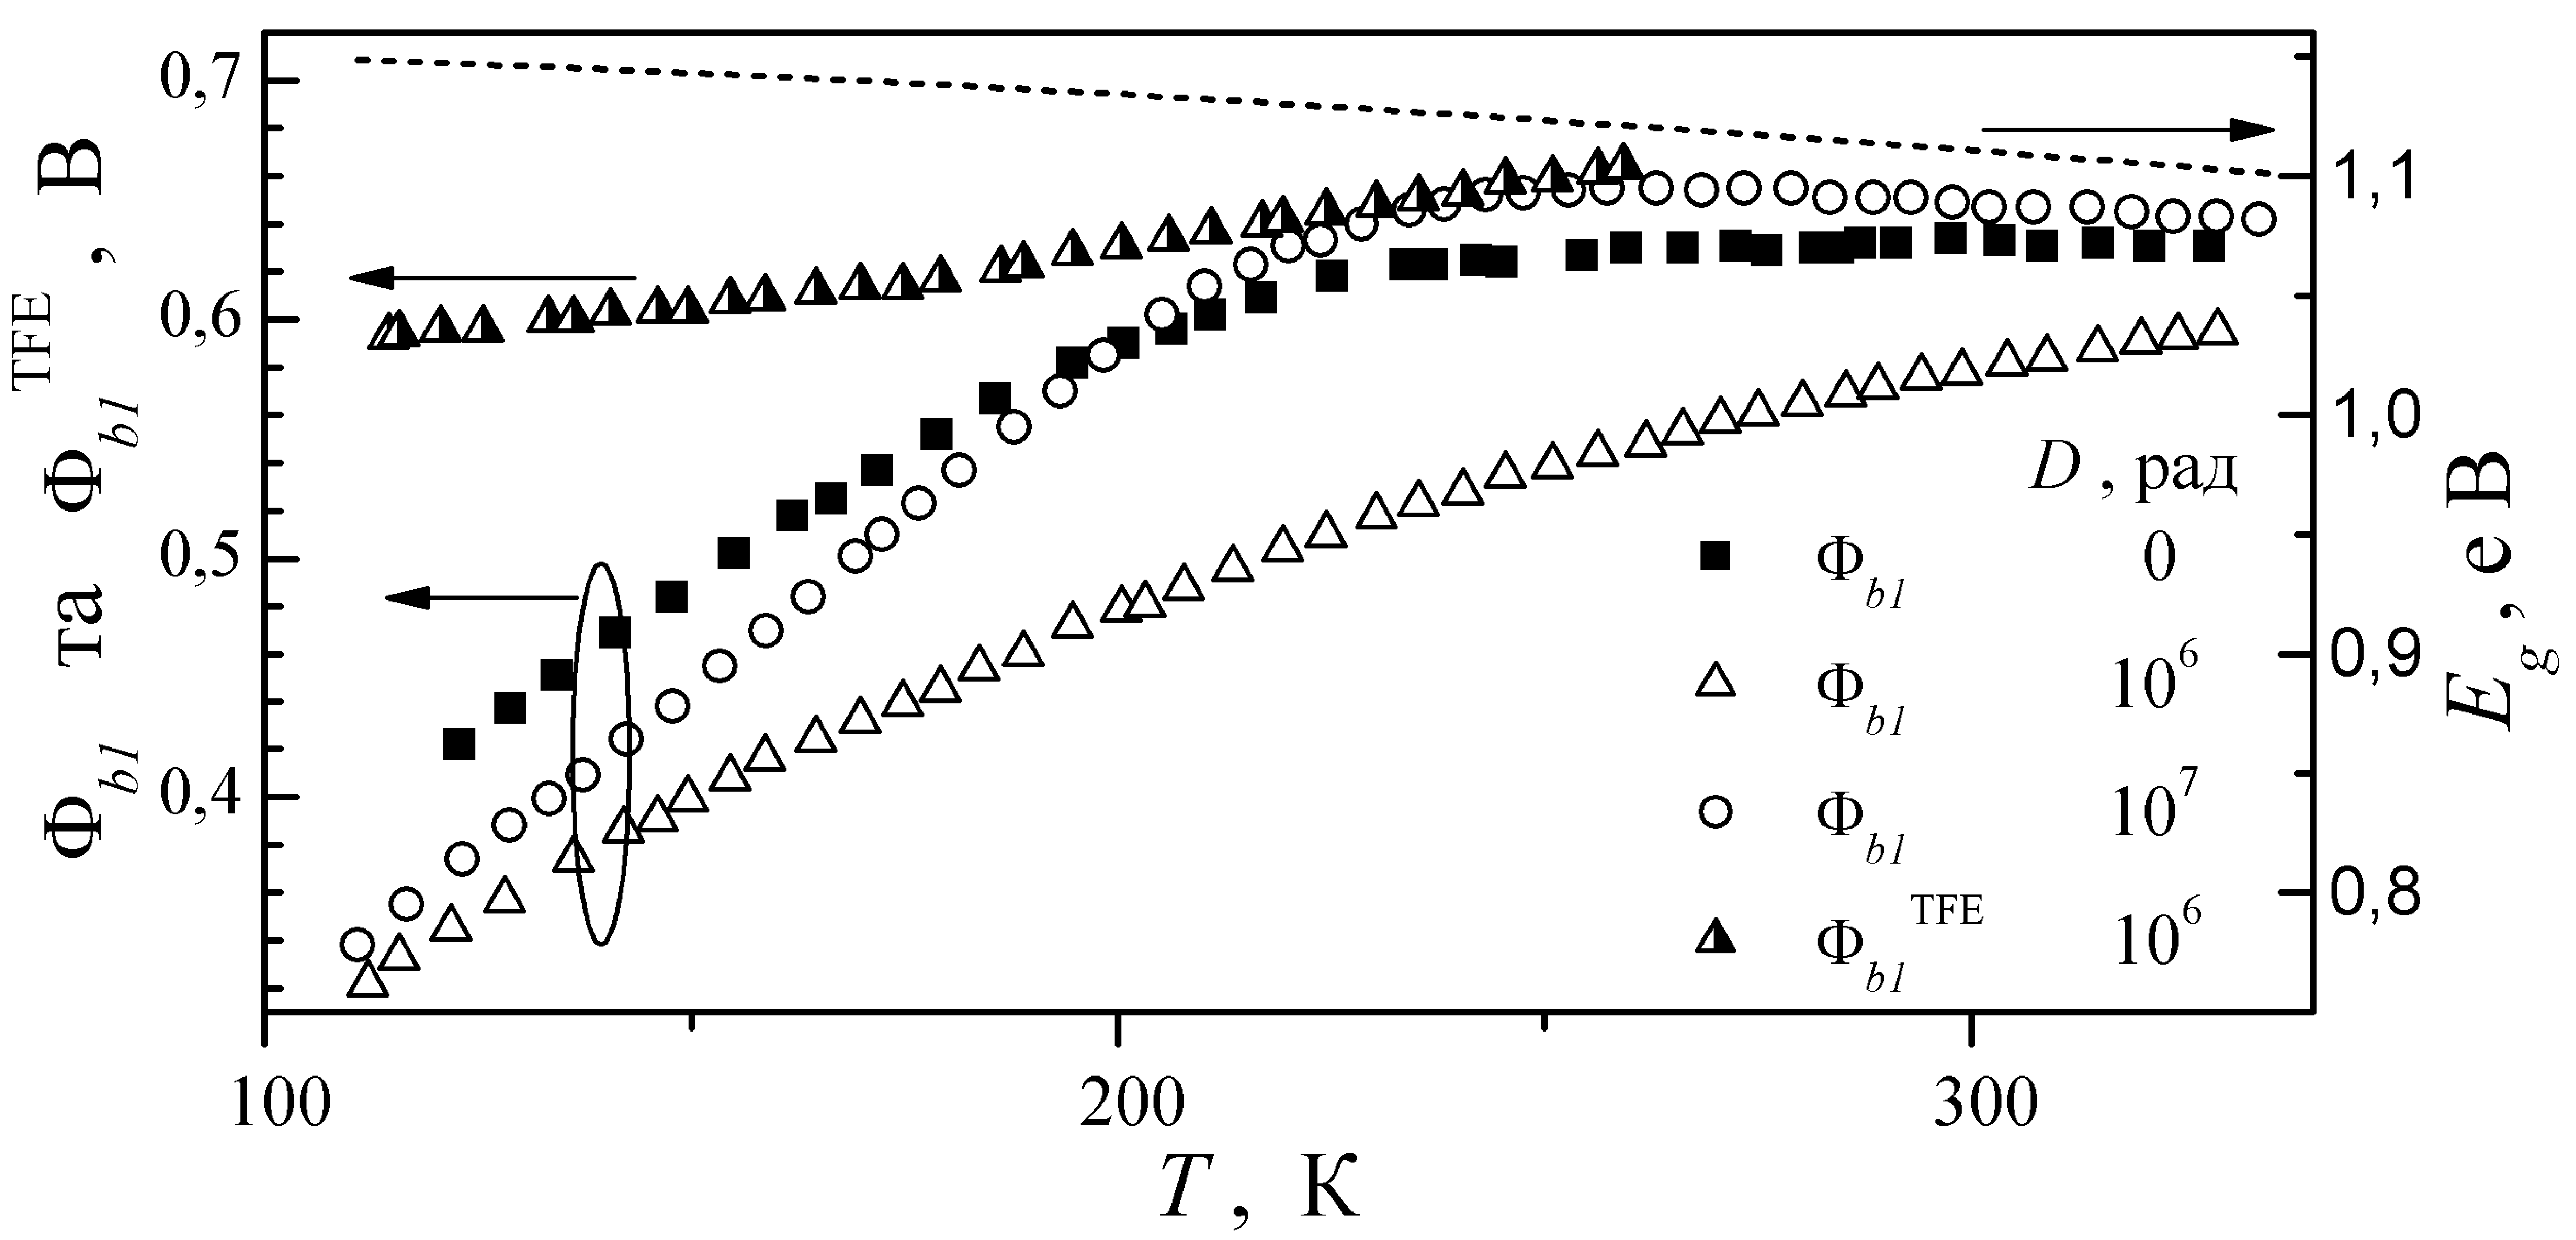
\includegraphics[width=0.7\textwidth]{figFbTrad_SDA}
\caption{\label{figFbTrad_SDA}
Температурні залежності висоти бар'єру структур Al$-n-n^+$--Si---Al.
Пунктирна лінія --- залежність ширини забороненої зони кремнію
}%
\end{figure}

Показано, що при зворотних зміщеннях струм $I_R$ складається з двох компонент --- рис.~\ref{figIVrg0USL_SDA},а).
Перша з яких, $I_\mathrm{TE}$, пов'язана з ТЕ процесами через неоднорідний контакт:
$I_\mathrm{TE}\sim T^2\exp(-E_\mathrm{TE}/kT)$,
$E_\mathrm{TE}\sim V_R^{2/3}$,
$V_R$ --- зворотна напруга.
Друга, $I_\mathrm{FN}$, --- не залежить від температури і пов'язана з процесами тунелювання за участю
центру з енергетичним положенням $E_c-(120\pm5)$~меВ, пов'язаним, найімовірніше, з міжвузольним атомом вуглецю С$_i$.
Внесок ТЕ складової зростає при підвищенні $T$ та зменшенні $V_R$.

\begin{figure}[b]
\center
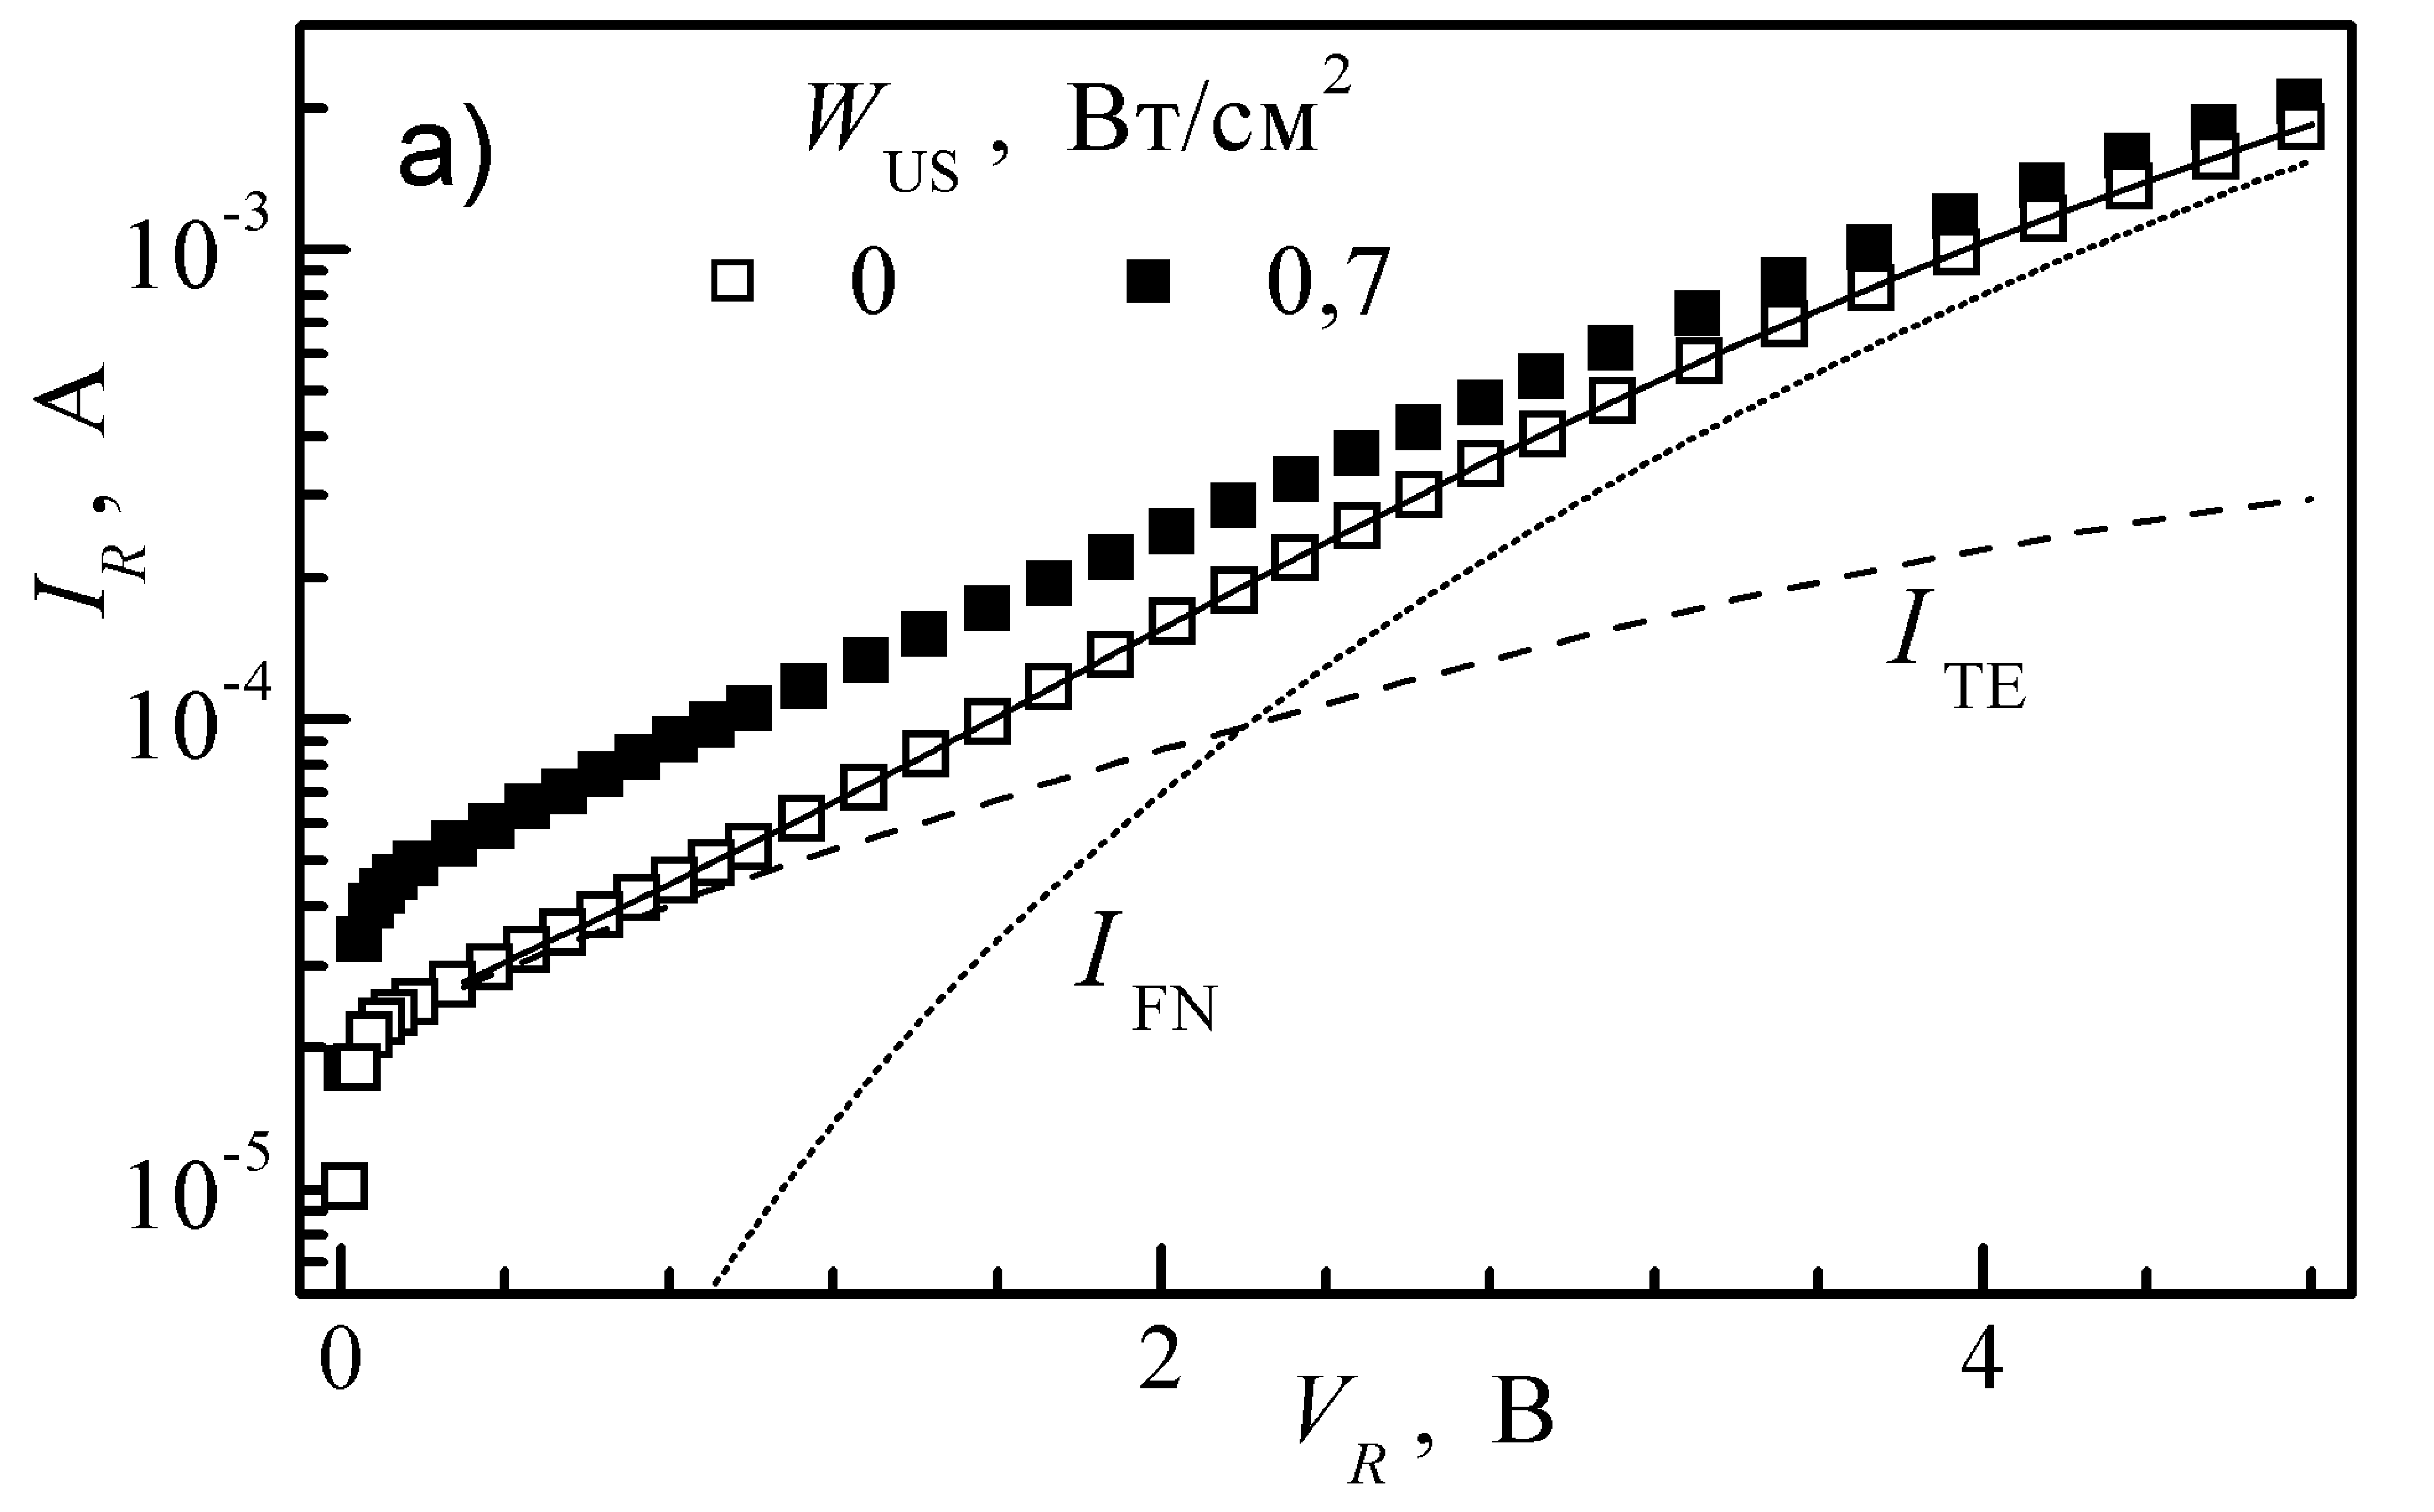
\includegraphics[width=0.33\textwidth]{figIVrg0USL_SDA}\hfill
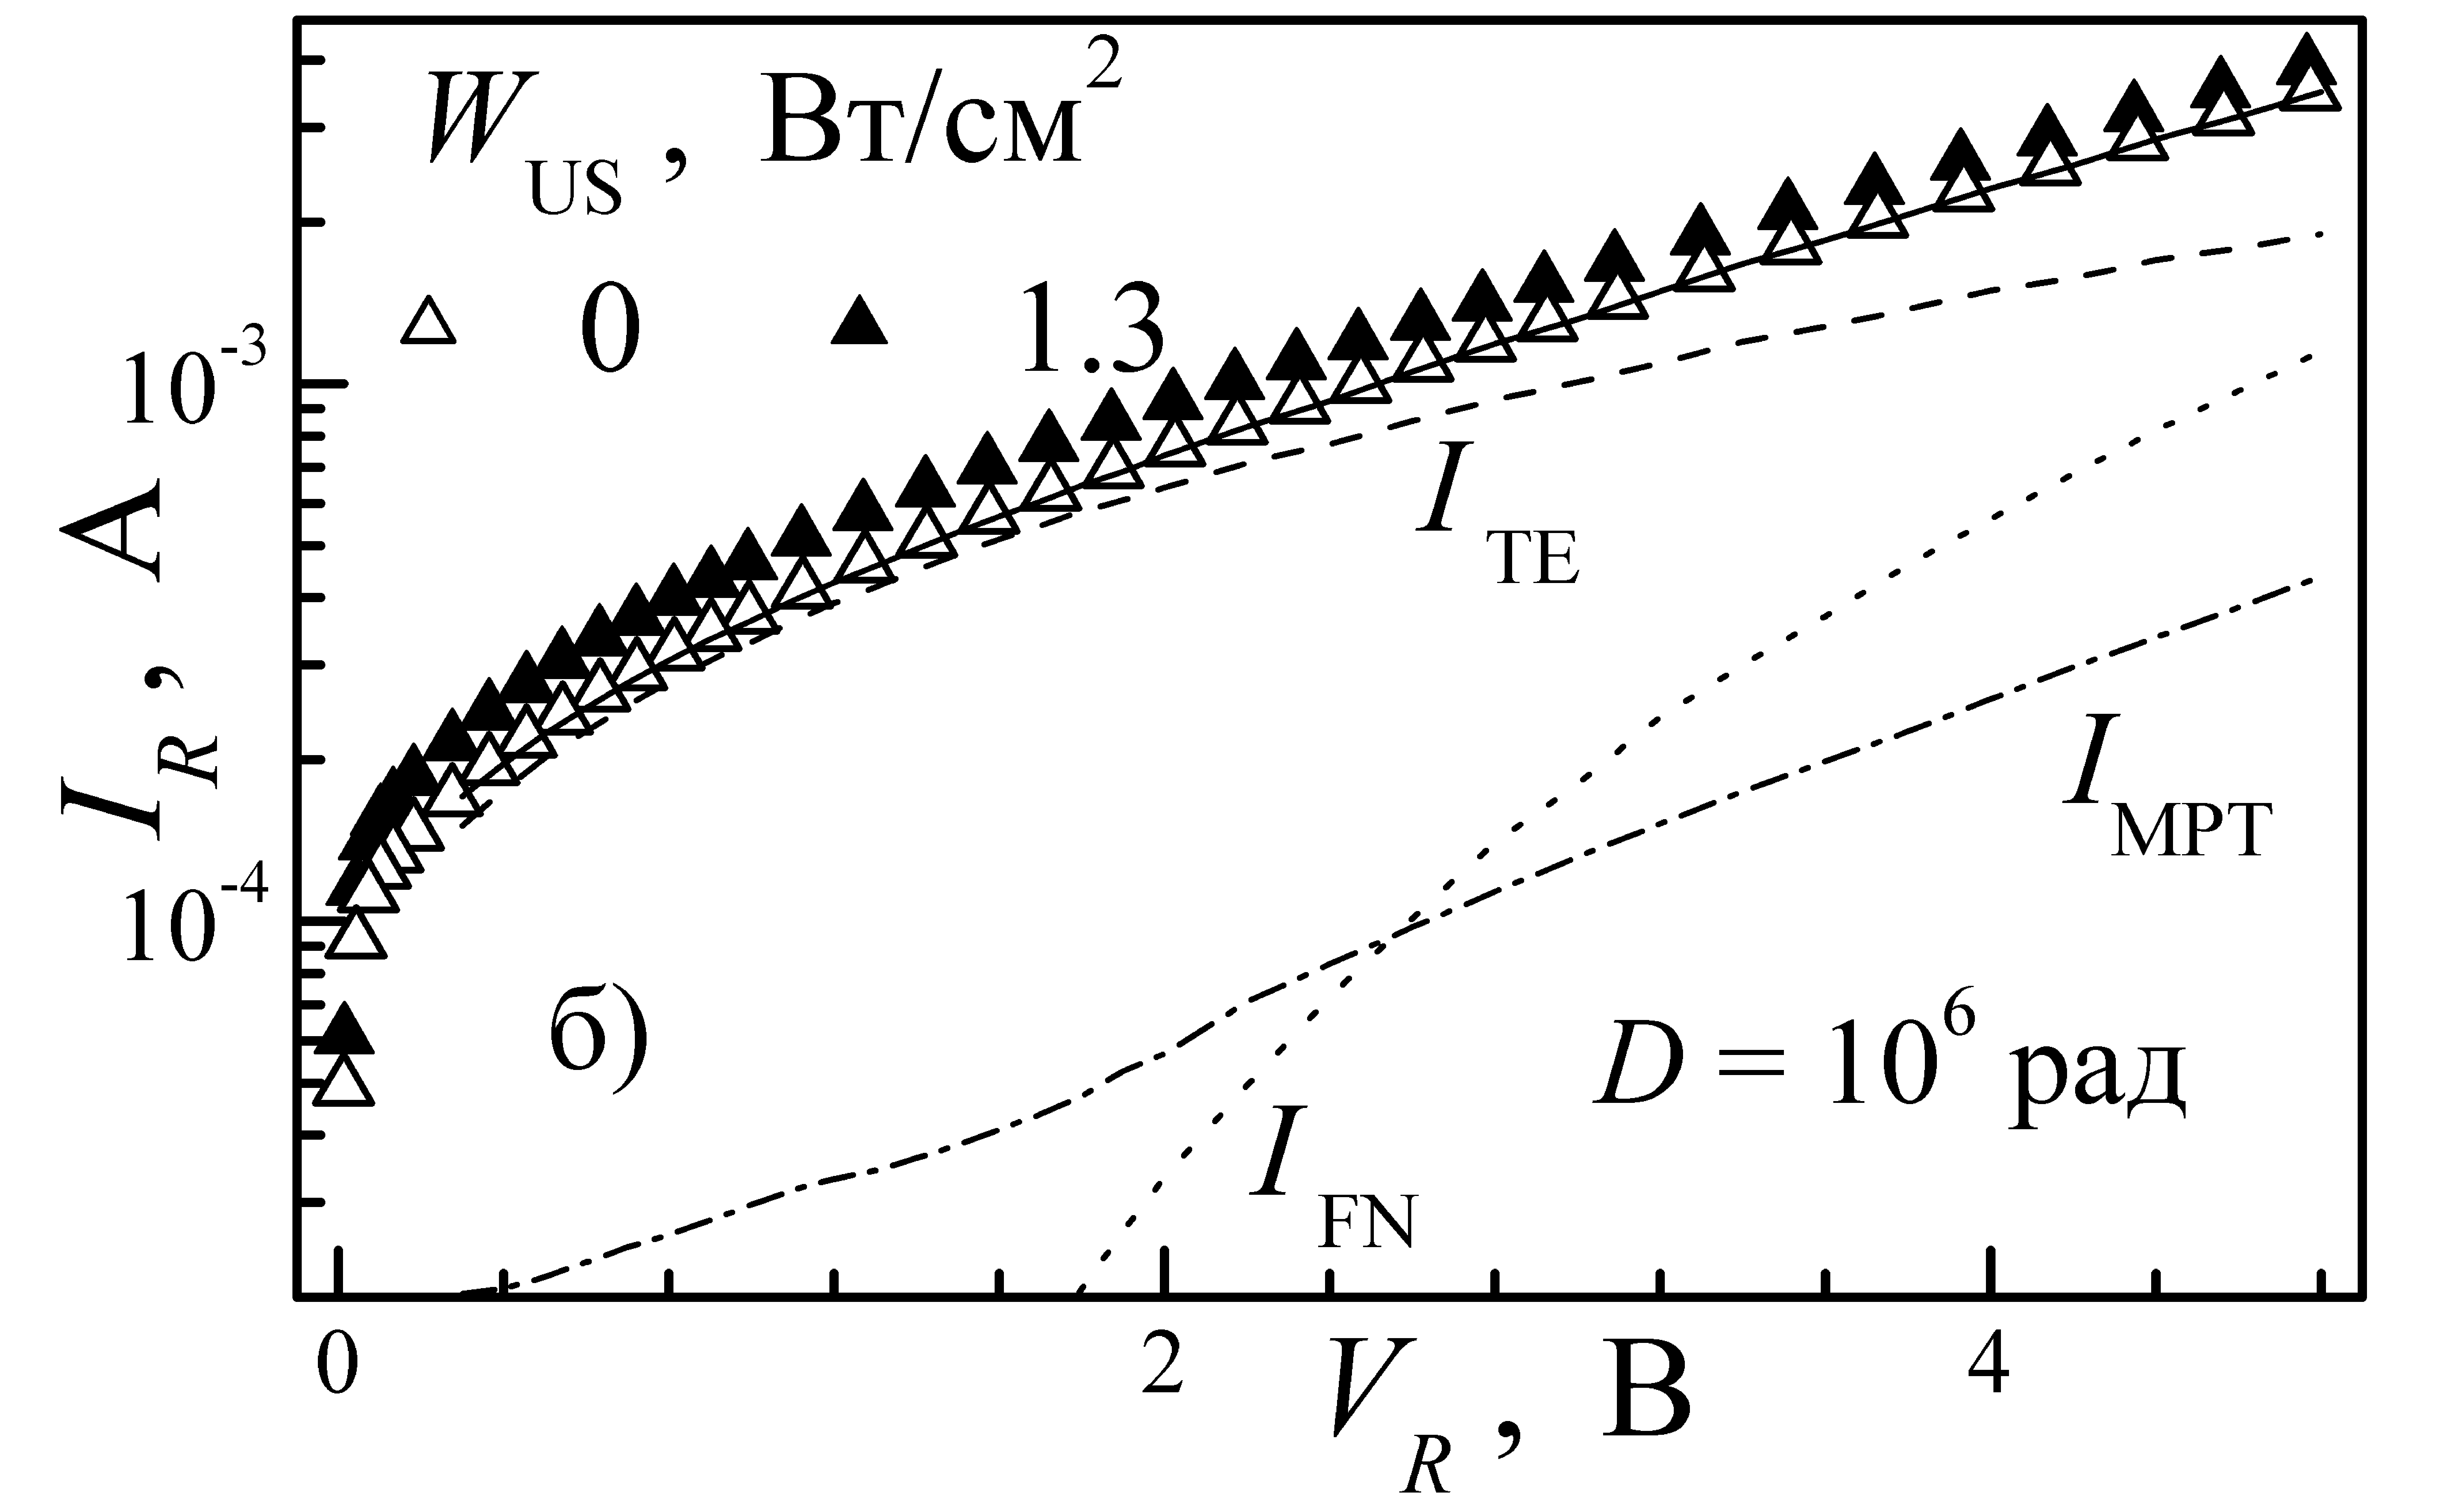
\includegraphics[width=0.33\textwidth]{figIVrg6USL_SDA}\hfill
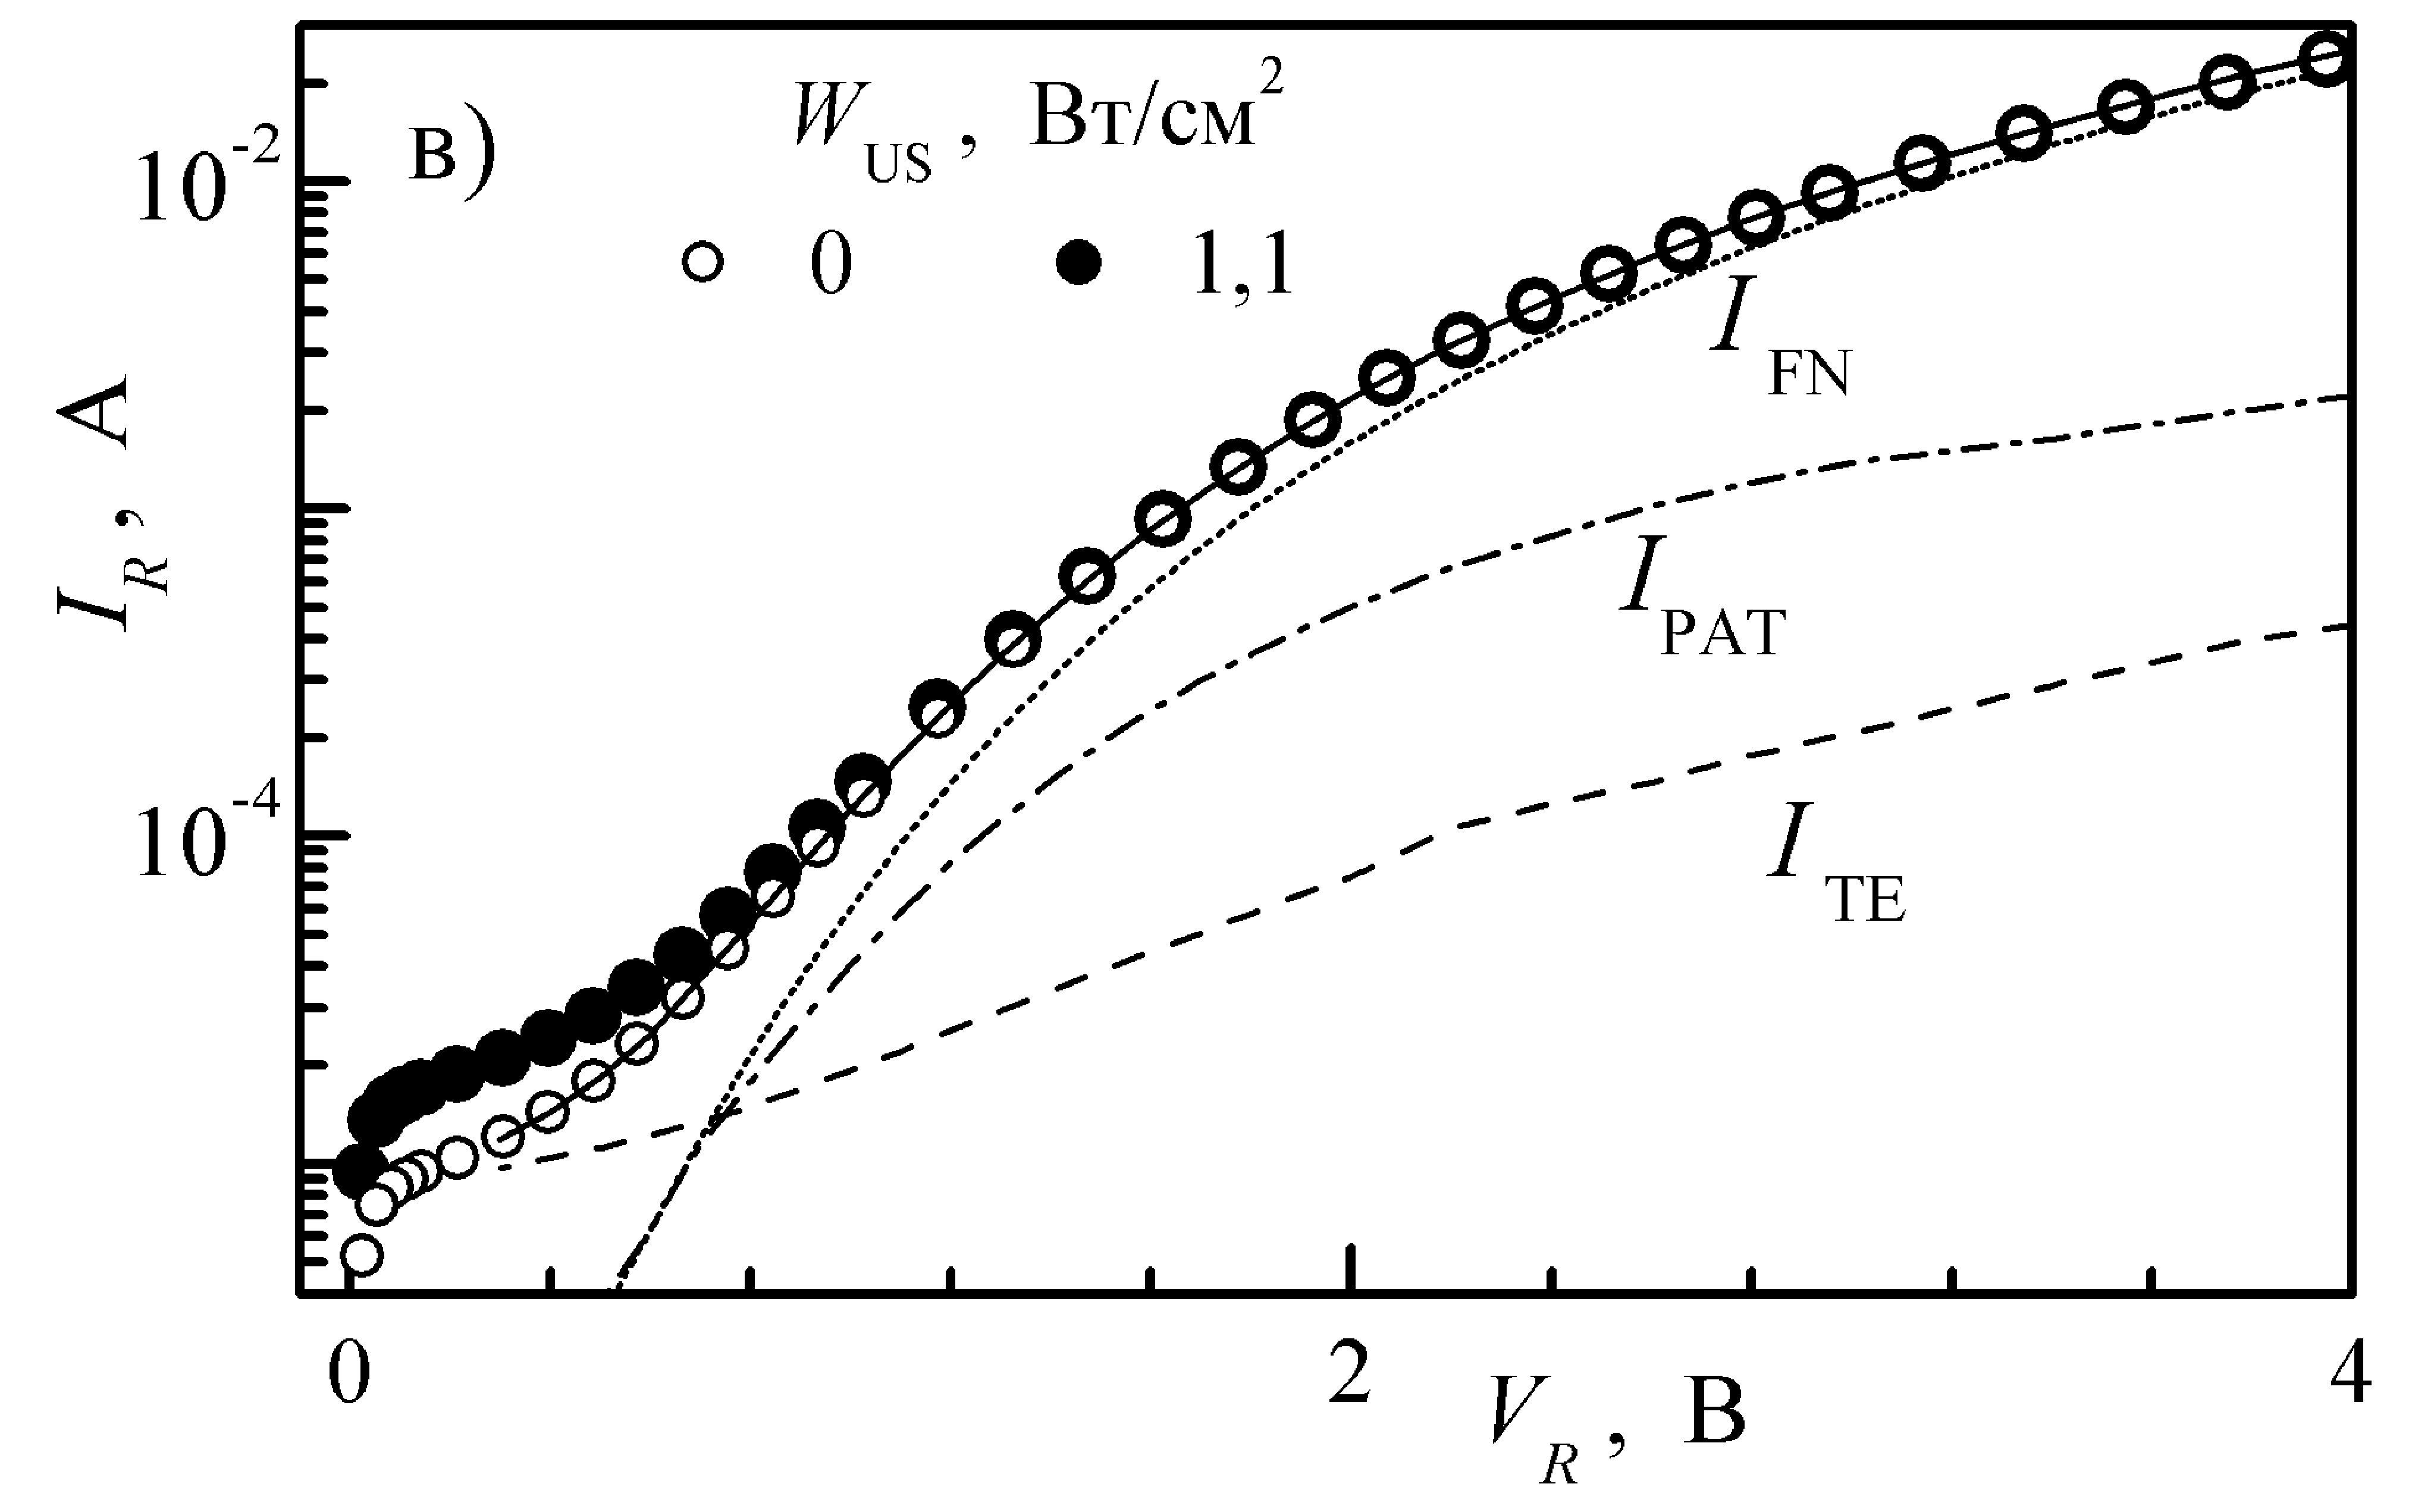
\includegraphics[width=0.33\textwidth]{figIVrg7USL_SDA}
\caption{\label{figIVrg0USL_SDA}
Зворотні  ВАХ  структур Al$-n-n^+$--Si---Al з різним ступенем опромінення.
$T=305$~K.
Заповнені та порожні точки відповідають вимірам за умов УЗН та без нього, відповідно.
$f_\mathtt{US}=9,6$~МГц.
Розривні відображають окремі складові зворотного струму для ненавантажених структур,
суцільні --- їх суму
}%
\end{figure}

Досліджено також структури Al$-n-n^+$--Si---Al, опромінені $\gamma$--квантами $^{60}$Co з $D=10^6$~рад та $D=10^7$~рад.
Виявлено, що ВБШ немонотонно змінюється зі збільшенням $D$ --- рис.~\ref{figFbTrad_SDA}.
Зауважимо, що в літературі і раніше повідомлялося подібні немонотонні дозові залежності $\Phi_{b}$, причому зустрічаються повідомлення про немонотонності двох типів (<<спад--зростання>> чи <<зростання--спад>>).
При зворотному зміщенні в опромінених структурах з'явилась додаткова компонента струму, $I_\mathrm{MPT}$, внесок якої зростає з підвищенням дози.
Температурні та польові залежності дозволили ідентифікувати $I_\mathrm{MPT}$ як струм, пов'язаний з тунельною багатофононною іонізацією глибоких домішкових центрів
%\cite{Ganichev:2000}
[6$^*$].
Крім того, для структур з $D=10^7$~рад, на відміну від меншої дози, суттєво зріс струм $I_\mathrm{FN}$.

Показано, що при $D=10^6$~рад домінуючим механізмом перенесення заряду при $120\div240$~K як при прямому зміщенні, так і при зворотному стає тунелювання за участю рівнів у забороненій, що пов'язано з утворенням радіаційних дефектів (РД).
При $T>260$~K основним механізмом залишається ТЕ через неоднорідний контакт, проте значення $\Phi_b^0$ та $\sigma_{\Phi}$
зростають до 0,772~В та 0,1~В, відповідно.
Поява при низьких температурах додаткового струму, як і для неопромінених структур, пов'язана з ефективним проходженням носіїв через області зниженого бар'єру,
причому загальна площа патчів не змінилась, проте зросла висота бар'єру (з 54 до 74~мВ).
Причиною змін ВБШ може бути накопичення на інтерфейсній границі РД акцепторного типу.
Причиною появи патчів є лінійні дефекти; збільшення $\sigma_{\Phi}$ пов'язане з  радіаційно--підсиленим дислокаційним ковзанням,
яке викликає а їх часткове перегрупування з утворенням більших за розміром скупчень
Збільшення впливу патчів маскує зростання ВБШ за їх межами і викликає ефективне зменшення висоти бар'єру, яка визначається безпосередньо з ВАХ (рис.~\ref{figFbTrad_SDA}).

При збільшенні дози до $10^7$~рад тунельний струм стає переважаючим не лише при зворотному зміщенні практично у всьому дослідженому температурному інтервалі,
але й при прямому зміщенні при $T=150\div220$~K.
При вищих температурах ($T=260\div330$~K) прямий струм пов'язаний як з тунелюванням, так і з ТЕ процесами через однорідний бар'єр висотою близько 710~мВ.
Це пов'язано з суттєвим збільшенням РД та ефективним гетеруванням патчами від'ємно заряджених дефектів.
Останнє призводить до
а)~того, що патчі почали виконувати роль тунельних шунтів і перестали впливати на процеси ТЕ.
б)~зменшення $\Phi_b$ в однорідній області, проте ефективна ВБШ, яка визначається безпосередньо з ВАХ, збільшилась порівняно з  $D=10^6$~рад.
Тобто характер немонотонності залежності $\Phi_b(D)$ залежить від ступеня неоднорідності:
для переважної площі контакту області має місця <<зростання--спад>>, проте ефект може маскуватися внаслідок впливу патчів.

Повідомляється про виявлені оборотні зміни характеристик структур Al$-n-n^+$--Si---Al під дією УЗН при $T=305$~К.
УЗН викликає зменшення ВБШ (рис.~\ref{figFbTrad_SDA},а), причому
а)~залежність $\Phi_b(W_\mathtt{US})$ в неопромінених структурах має пороговий характер;
б)~після $\gamma$--опромінення ефективність впливу УЗ знижується і змінюється характер амплітудної залежності;
в)~зі збільшення $D$ зростають величини АІ змін.
Показано, що в неопромінених структурах зменшення ВБШ пов'язане зі зміною рівень нейтральності інтерфейсних станів
внаслідок іонізації дефектів на границі розділу, викликане АІ коливаннями дислокаційних відрізків.
Опромінення викликає
а)~закріплення сегментів лінійних дефектів внаслідок гетерування РД;
б)~появу АА точкових РД (А--центри, дивакансії)
що і спричинює зміну механізму акусто--дефектної взаємодії.
Незначні АІ зміни фактора неідеальності спостерігаються лише у випадку, коли $n_\mathtt{id}>1,1$ (рис.~\ref{figFbTrad_SDA},б),
що пов'язано з впливом УЗ та стан патчів внаслідок взаємодії з РД, захопленими в областях неоднорідності.

\begin{figure}
\center
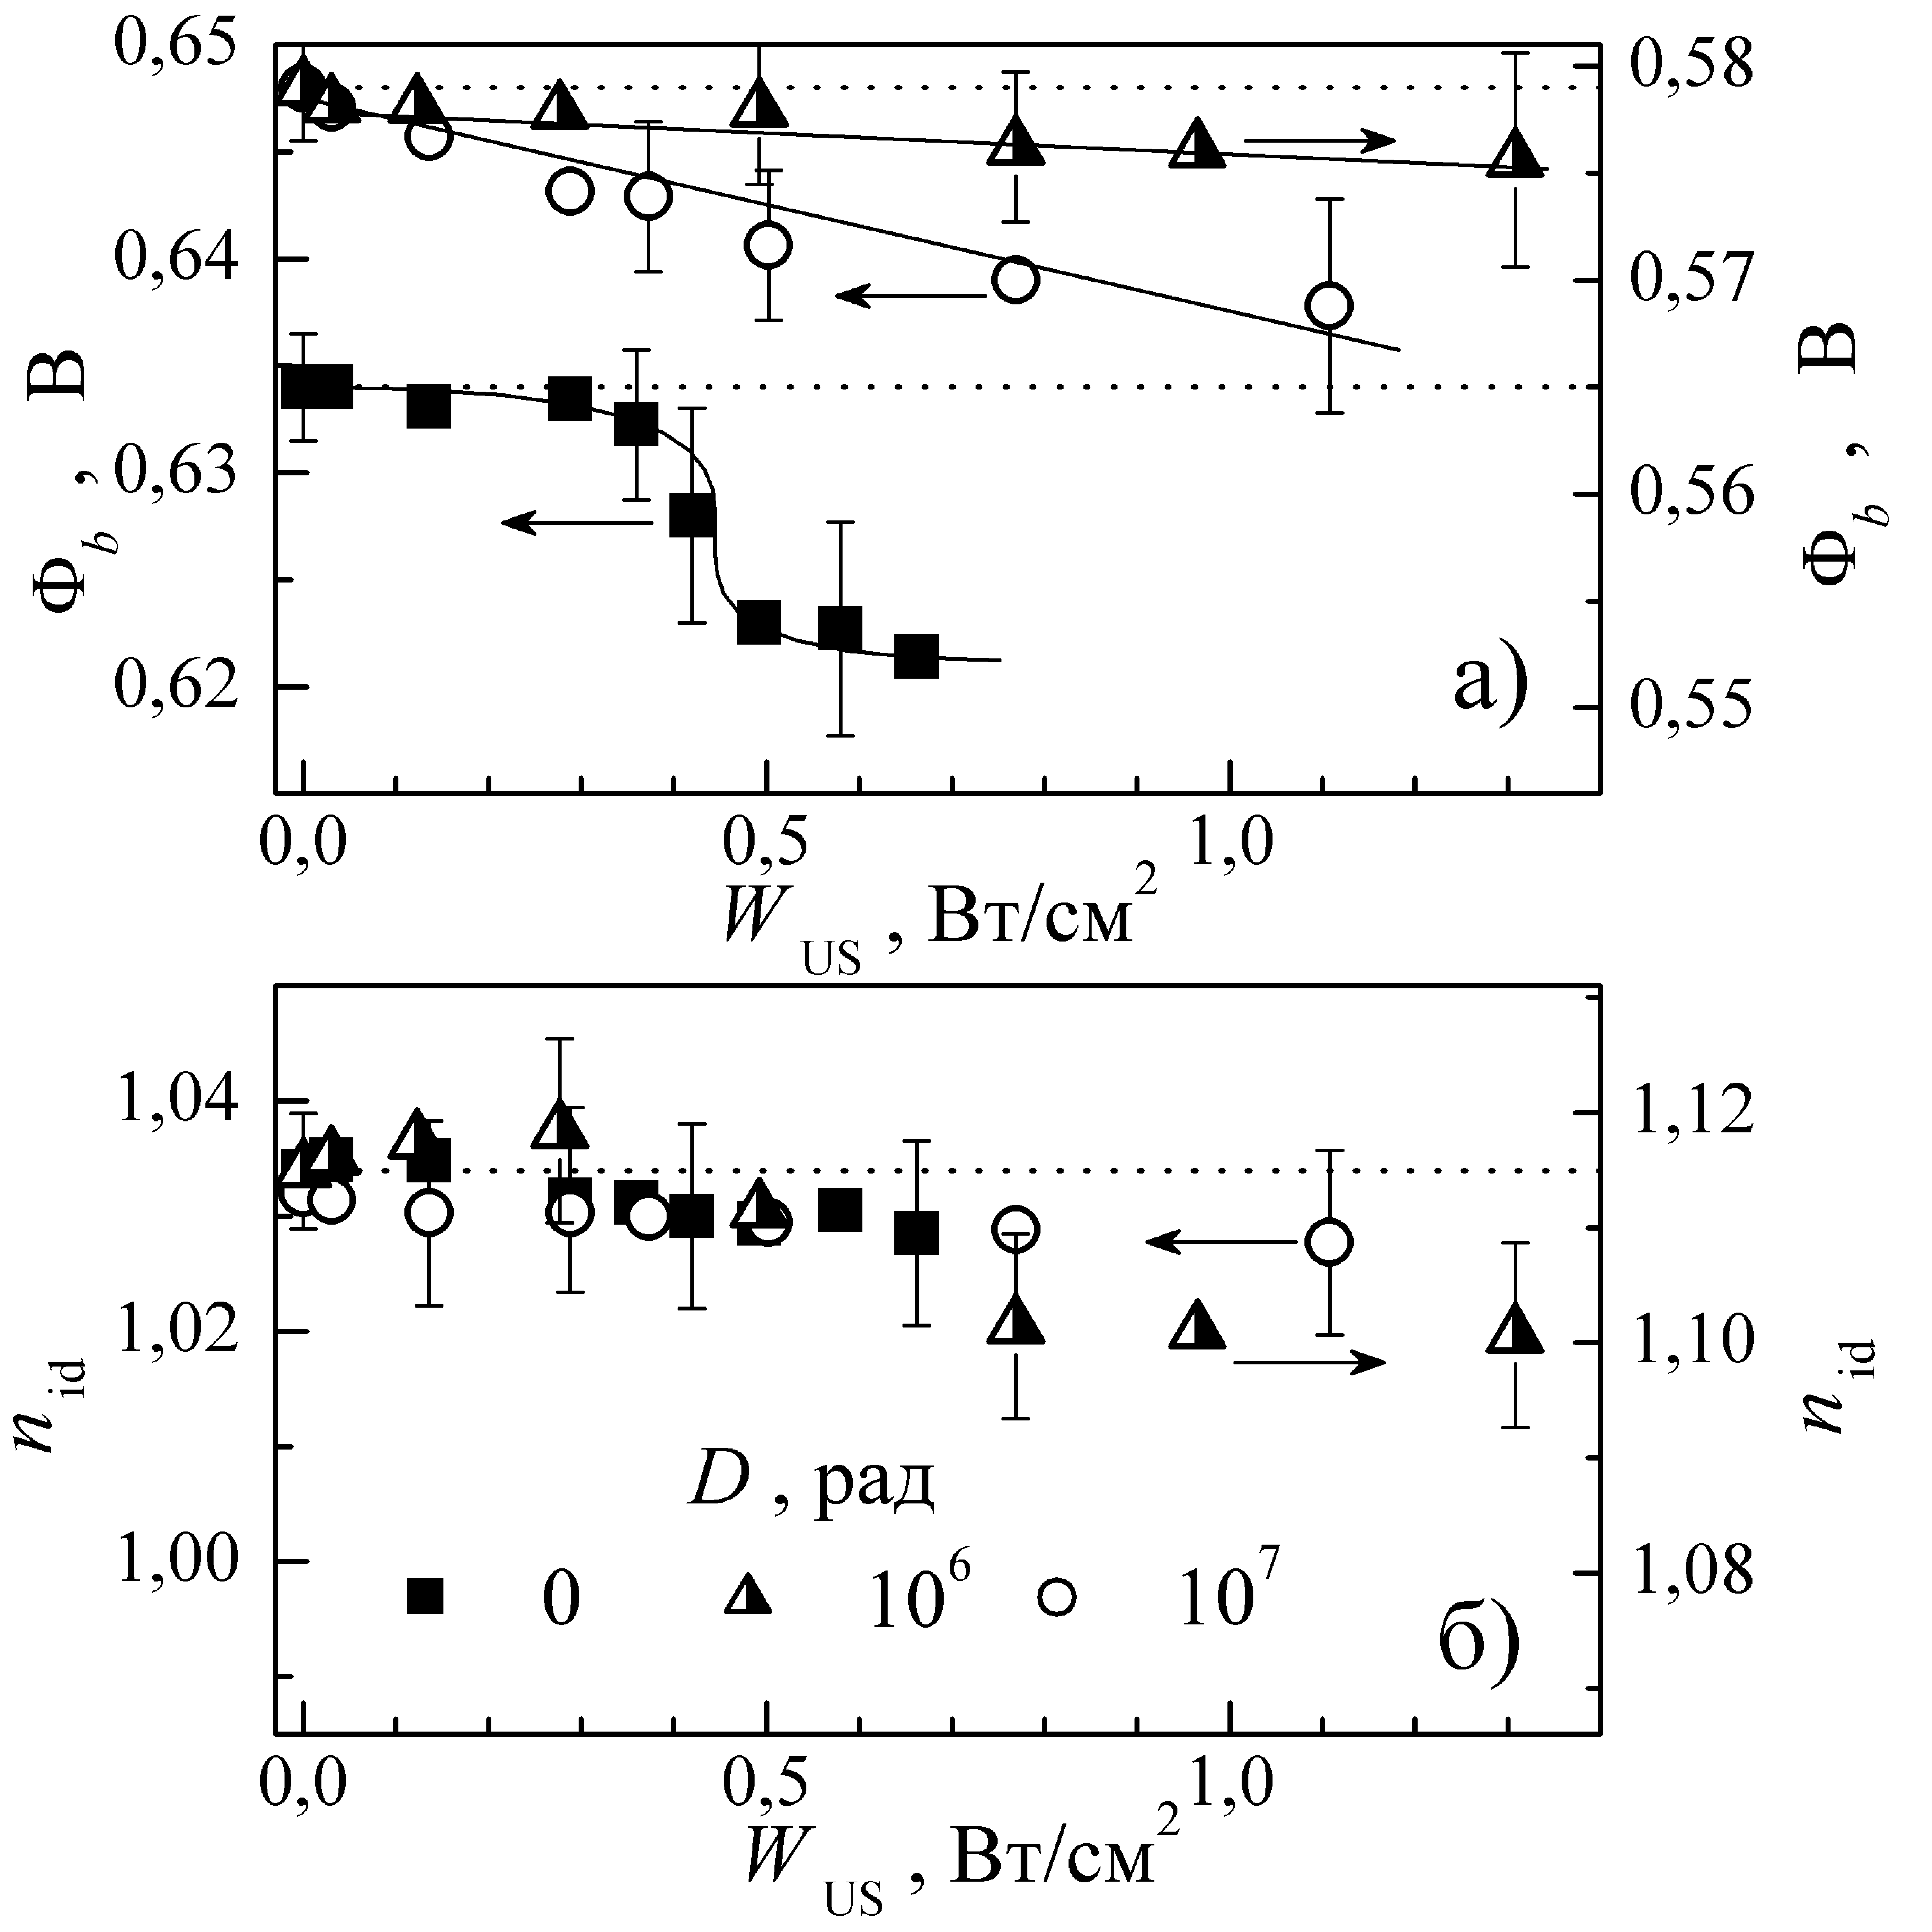
\includegraphics[width=0.6\textwidth]{figFbUSL_SDA}
\caption{\label{figFbUSL_SDA}
Залежності висоти бар'єру Шотткі (а) та фактора неідеальності (б)  від інтенсивності УЗ для
структур Al$-n-n^+$--Si---Al з різним ступенем опромінення.
$T=305$~K.
$f_\mathtt{US}=9,6$~МГц.
Горизонтальні пунктирні лінії відповідають значенням параметрів, виміряних без УЗН
}%
\end{figure}

За умов УЗН спостерігається збільшення (до декількох десятків відсотків) величини зворотного струму --- рис.~\ref{figIVrg0USL_SDA}.
Ефект послаблюється зі збільшенням зміщення, амплітудна залежність як для неопромінених, так і опромінених структур аналогічна АІ змінам ВБШ.
Останнє може бути використано для створення сенсору $\gamma$--опромінення,
робота якого грунтуватиметься на вимірюванні АІ змін величини $I_R$ хоча б при двох значеннях $W_\mathtt{US}$,
одне з яких більше, а інше менше порогу для неопроміненого зразка.
Відношення отриманих величин дозволить зробити висновок про сам факт опромінення,
а безпосереднє значення зміни при більшій інтенсивності УЗ залежить від дози.
Показано, що АІ зміни $I_R$ пов'язані з впливом пружних хвиль лише на ТЕ складову,
тоді як незмінність при УЗН складових струму, пов’язаних з прямим та багатофононним тунелюванням,
свідчить що відповідні дефекти (зокрема С$_i$) не є акустоактивними.


У  \underline{\textbf{п'ятому розділі}} представлені результати досліджень
оборотних АІ ($f_\mathtt{US}=4,1$, 8,4 та 27,8~МГц) змін параметрів діодів Шотткі Mo$/n-n^+$--Si в широкому ($130\div330$~К) температурному діапазоні.
Зауважимо, що до початку роботи бар'єрні структури на основі малодислокаційних неп'єзоелектричних напівпровідникових кристалів
залишалися поза увагою науковців з точки зору дослідження низькотемпературних АІ ефектів.

\begin{figure}
\center
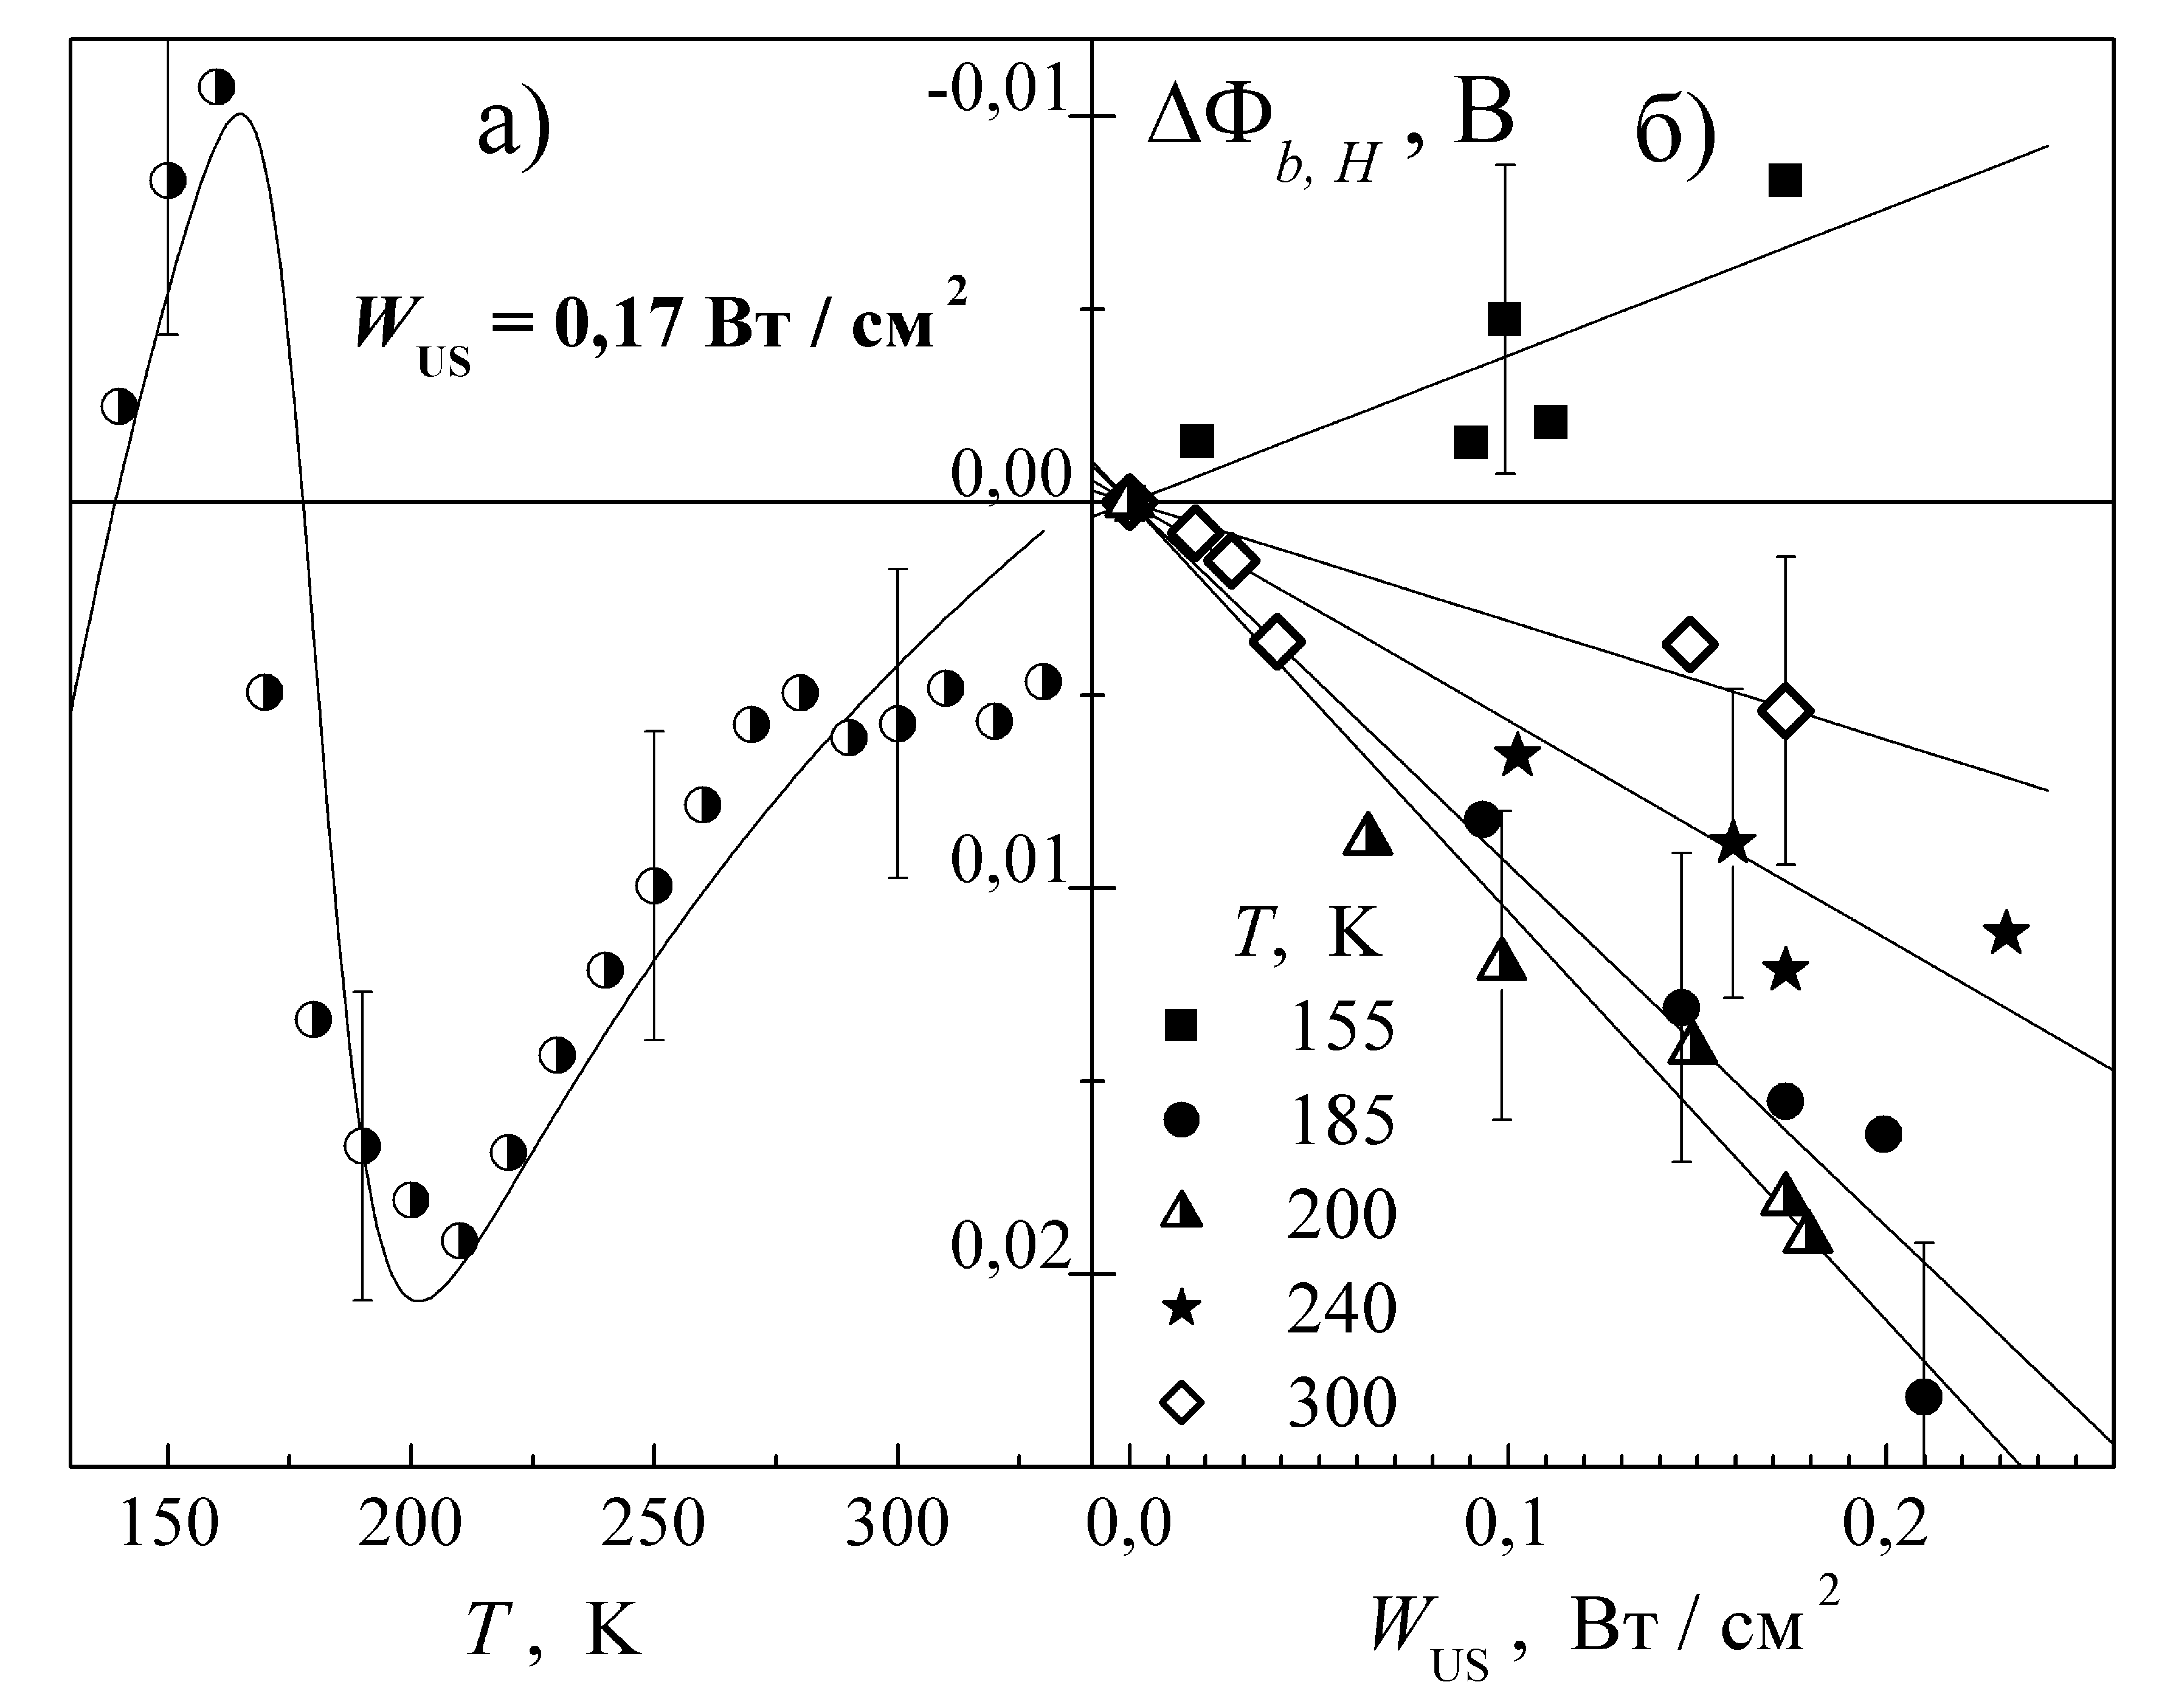
\includegraphics[width=0.6\textwidth]{figDelFbH}
\caption{\label{figDelFbH}
Залежності АІ змін висоти бар'єру високотемпературної компоненти струму від температури (а) та інтенсивності введеного УЗ (б).
$f_\mathtt{US}=4,1$~МГц
}%
\end{figure}

Апроксимація (метод МАВС) прямих гілок ВАХ проводилася відповідно до виразу
\begin{equation}
\label{eqSDB_IV}
  I=I_{s,H}\left[\exp\left(\frac{qV}{n_\mathrm{id,H}kT}\right)-1\right]+
 I_{s,L}\left\{\exp\left[\frac{q(V-IR_s)}{n_\mathrm{id,L}kT}\right]-1\right\},
\end{equation}
тобто струм складається з високотемпературної компоненти (ВТКС, перший доданок), яка при низьких температурах переважала лише при великих зміщеннях та низькотемпературної (НТКС, другий доданок),
яка спостерігалася лише при $T<220$~К.
Показано, що перенесення заряду відбувається відповідно до моделі ТЕ через неоднорідний контакт,
причому для опису ВБШ за межами патчів (пов'язаного з ВТКС) доцільно застосовувати наближення подвійного розподілу Гауса
%\cite{Jiang:DG}
[7$^*$]:
\begin{equation}
\label{eqDG}
  \Phi_{b,H}=-\frac{kT}{q}\ln\left[\varrho_1\exp\left(-\frac{q\Phi_{b,1}^0}{kT}+
  \frac{q^2\sigma^2_{\Phi,1}}{2k^2T^2}\right)
   +
  \varrho_2\exp\left(-\frac{q\Phi_{b,2}^{0}}{kT}+
  \frac{q^2\sigma^2_{\Phi,2}}{2k^2T^2}\right)\right],
\end{equation}
$\varrho_1$, $\varrho_2$  --- вагові коефіцієнти кожного з розподілів.
Виявлено, що для ВТКС ультразвук викликає оборотні збільшення фактора неідеальності та зміни ВБШ,
величина і знак яких залежить від температури --- рис.~\ref{figDelFbH}.
Розрахунки, проведені відповідно до моделі
%\cite{Tung:MSE,Jiang:DG}
[3$^*$,7$^*$] показали, що за умов УЗН відбувається зростання
$\Phi_{b,1}^0$ (від 780~мВ до, наприклад при $f_\mathtt{US}=4,1$~МГц, $W_\mathtt{US}=0,17$~Вт/см$^2$,  810~мВ),
$\Phi_{b,2}^0$ (від 1100 до  1200~мВ),
$\sigma_{\Phi,1}$ (від 20 до  50~мВ),
$\sigma_{\Phi,2}$ (від 120 до  130~мВ) та
зростання внеску другого розподілу (в чотири рази).
Аналіз НТКС показав, що УЗН викликає зміни ВБШ в області патчів, які немонотонним чином залежать від $W_\mathtt{US}$,
зростання (від від 0,2 до 2~мм$^{-2}$) ефективної густини патчів та зменшення (від $2,7\cdot10^{-5}$ до $2,5\cdot10^{-5}$ м$^{2/3}\cdot$В$^{1/3}$)
величини $3(R_p^2\Delta_p/4)^{1/3}$, де $\Delta_p$ та $R_p$ --- зниження висоти бар'єру в області патча та його розмір, відповідно.
Основні виявлені особливості впливу УЗН якісно показані на рис.\ref{figBand}.



\begin{figure}
\center
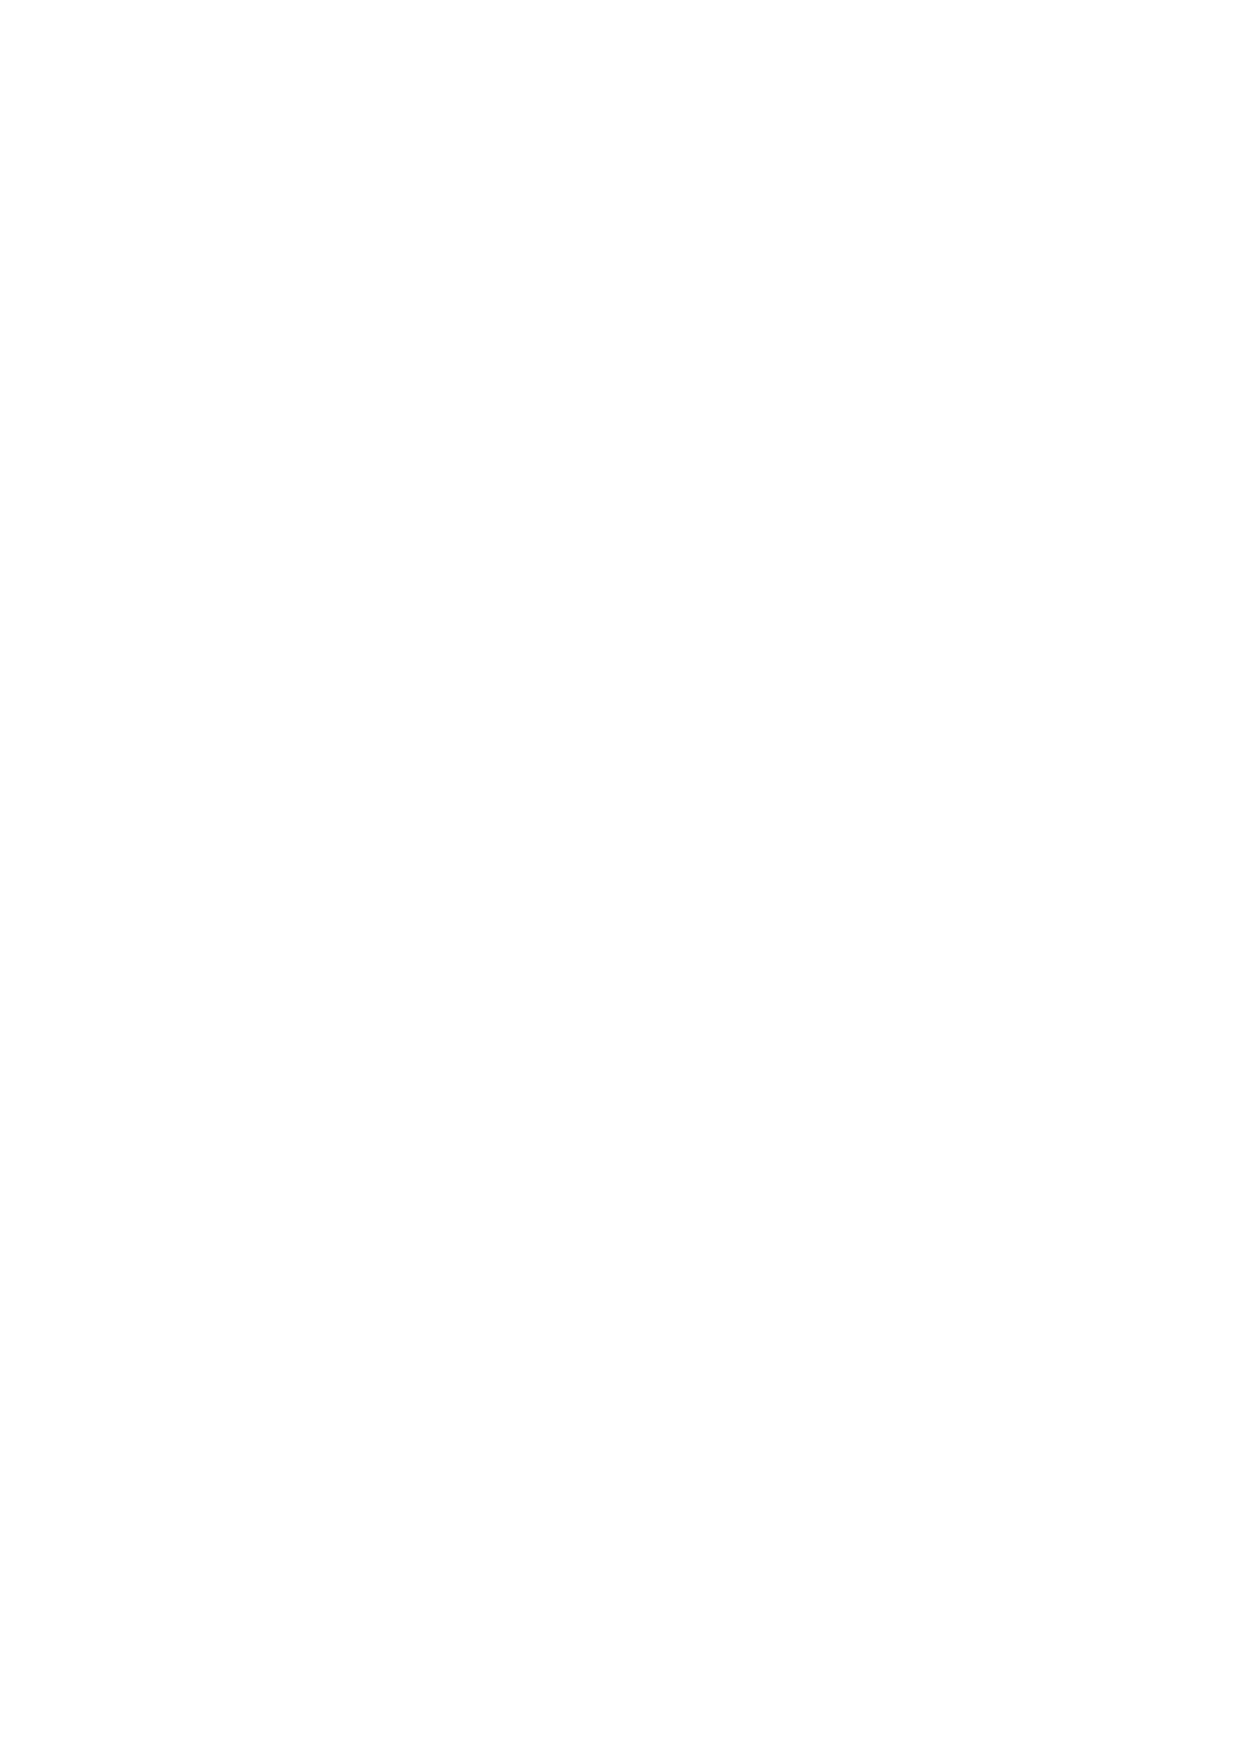
\includegraphics[width=0.55\textwidth]{figBand}
\caption{\label{figBand}
Схематичне зображення
просторового розподілу поверхневого потенціалу
%зони провідності,
що відображає різницю між випадком УЗН (верхня площина та верхня контурна поверхня) та
його відсутністю (нижня площина та нижня контурна поверхня).
Рисунок зроблено у припущенні, що наявні два патчі.
При розрахунку потенціальних поверхонь була використана формула~(1.5.3) з
%\cite{Tung:MSE}
[5$^*$]
}%
\end{figure}

\begin{figure}[b]
\center
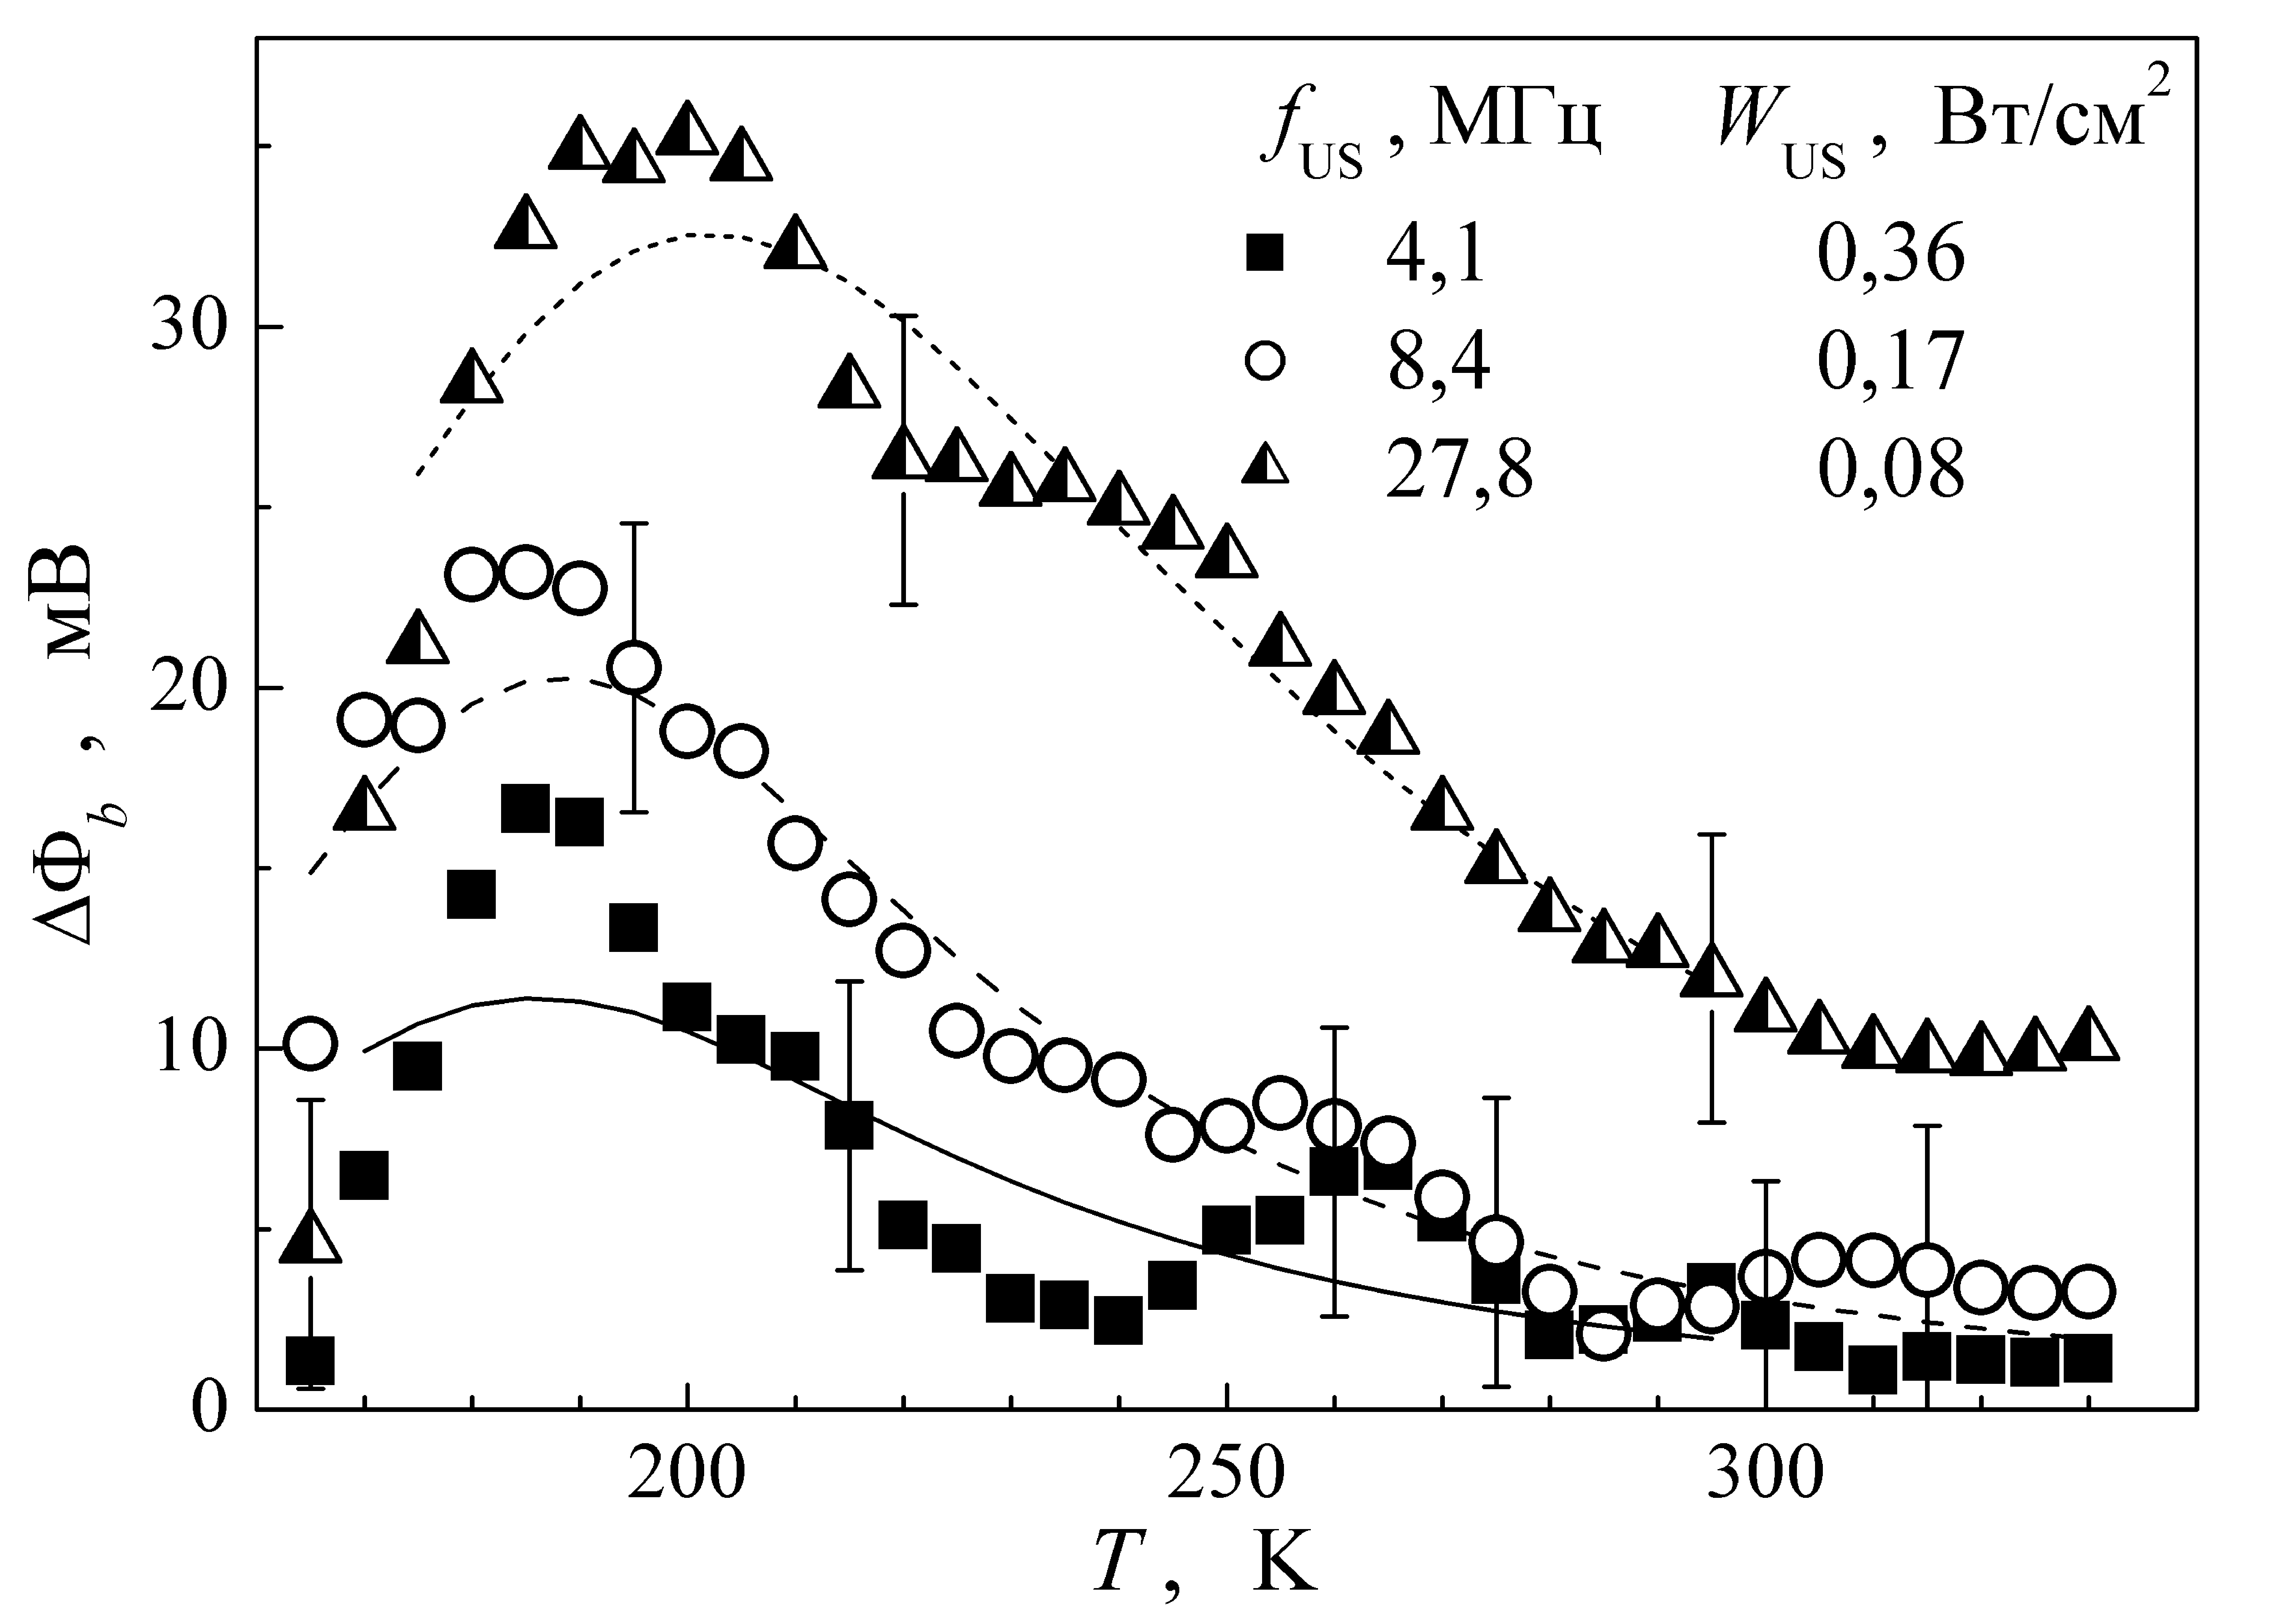
\includegraphics[width=0.6\textwidth]{figDelFbT_SDB}
\caption{\label{figDelFbT_SDB}
Температурні залежності АІ змін ВБШ при УЗН на різних частотах.
Точки --- експеримент,
лінії --- апроксимація згідно з формулою~(\ref{eqBr})
}%
\end{figure}
Визначені можливі механізмів акусто--дефектної взаємодії і показано, що температурні та частотні залежності АІ змін в структурах
 Mo$/n-n^+$--Si (рис.\ref{figDelFbT_SDB}) можуть бути пояснені в рамках моделі Брейсфолда
% \cite{Brailsford}
[8$^*$],
яка передбачає акстостимульовану дифузію перегинів лінійних дефектів.
Зокрема, залежності зміни ВБШ описуються виразом
\begin{equation}
\label{eqBr}
\Delta\Phi_{b,H}\,(f_\mathtt{US},\,T)\sim\frac{f_\mathtt{US}}{T}\frac{(f_\mathtt{US}/{f_k})\exp\left(\frac{W_k}{kT}\right)}
{1+(f_\mathtt{US}/{f_k})^2\exp\left(\frac{2W_k}{kT}\right)}W_\mathtt{US},
\end{equation}
де
$W_k$ --- енергія активації дифузії,
а параметр $f_k$ пов'язаний з середньою довжиною дислокаційного сегмента та абсолютним значенням коефіцієнта дифузії.
В досліджених структурах ці дефекти пов'язані з патчами,
визначені в рамках моделі величини становлять $W_k=(90\pm10)$~меВ та $f_k=(3\pm2)\cdot10^9$~Гц.


Проведені дослідження зворотного струму показали, що
а)~перенесення заряду пов'язане з процесами ТЕ та тунелюванням, стимулюваним фононами, носіїв з електронних станів поблизу границі розділу (РАТ)
%\cite{Pipinys2006}
[9$^*$]
і може бути описане виразом
\begin{eqnarray}
\label{eqIgen}
 I_R&=&I_{TE}+I_{P\!AT}=P_tI_0\,T^2\exp\left(-\frac{q\Phi_b}{kT}\right)\left[1-\exp\left(-\frac{V_s}{kT}\right)\right]+\\
 &&+\frac{P_tq^2F_mAN_{ss}}{\sqrt{8m^*\epsilon_t}}\left(1-\frac{\gamma}{\gamma_1}\right)^{1/2}\exp
    \left\{-\frac{4\sqrt{2m^*}\,\epsilon_t^{3/2}\left(\gamma_1-\gamma\right)^2}{3qF_m\hbar} \nonumber
    [\gamma_1+\frac{1}{2}\gamma]\right\}\\ \nonumber
%        P_t&=&\exp\left\{-\frac{4\sqrt{2m_i^*q}}{3\hbar V_i}\left[(U_0+V_i)^{\,3/2}-U_0^{\,3/2}\right]\delta\right\}\,,\\ \nonumber
    \gamma_1&=&(1+\gamma^2)^{1/2}, \quad
    %\\ \nonumber
    \gamma=\frac{a_\mathtt{e-ph}\hbar\omega_{ph}^2\sqrt{2m^*}}{qF_m\sqrt{\epsilon_t}}
    \left\{\frac{\exp\left(\frac{\hbar\omega_{ph}}{kT}\right)+1}{\exp\left(\frac{\hbar\omega_{ph}}{kT}\right)-1}\right\},   \nonumber
\end{eqnarray}
де
$P_t$ --- ймовірність тунелювання через діелектричний прошарок,
$N_{ss}$ --- густина заповнених рівнів поблизу інтерфейсу,
$\hbar\omega_{ph}$ --- енергія фонону,
$a_\mathtt{e-ph}$ --- константа електрон--фононної взаємодії,
$\epsilon_t$ --- глибина залягання рівнів,
$F_m$ --- напруженість електричного поля на границі розділу МН;
б)~ВБШ та $\epsilon_t$ зменшуються при зростанні зворотної напруги
($\Phi_{b}=\Phi_{b0}-\alpha_{F} F_m$,
$\epsilon_t=\epsilon_{t0}-\beta_F F_m^{1/2}$), що пов'язано з впливом інтерфейсних станів
%\cite{Tung:MSE}
[5$^*$] та ефектом Пула--Френкеля.
в)~за умов УЗН зареєстроване оборотне зростання $I_R$, викликане АІ зменшенням параметрів (табл.~\ref{tabSDBParZv});
г)~причиною появи рівнів можуть бути кластери позитивно заряджених дефектів, а АІ змін $I_{P\!AT}$ --- модифікація розміру кластера, викликана
локальне підвищення температури скупчення дефектів в акустичному полі
%\cite{MirzadeJAP2011}
[2$^*$].

%\begin{figure}
%\center
%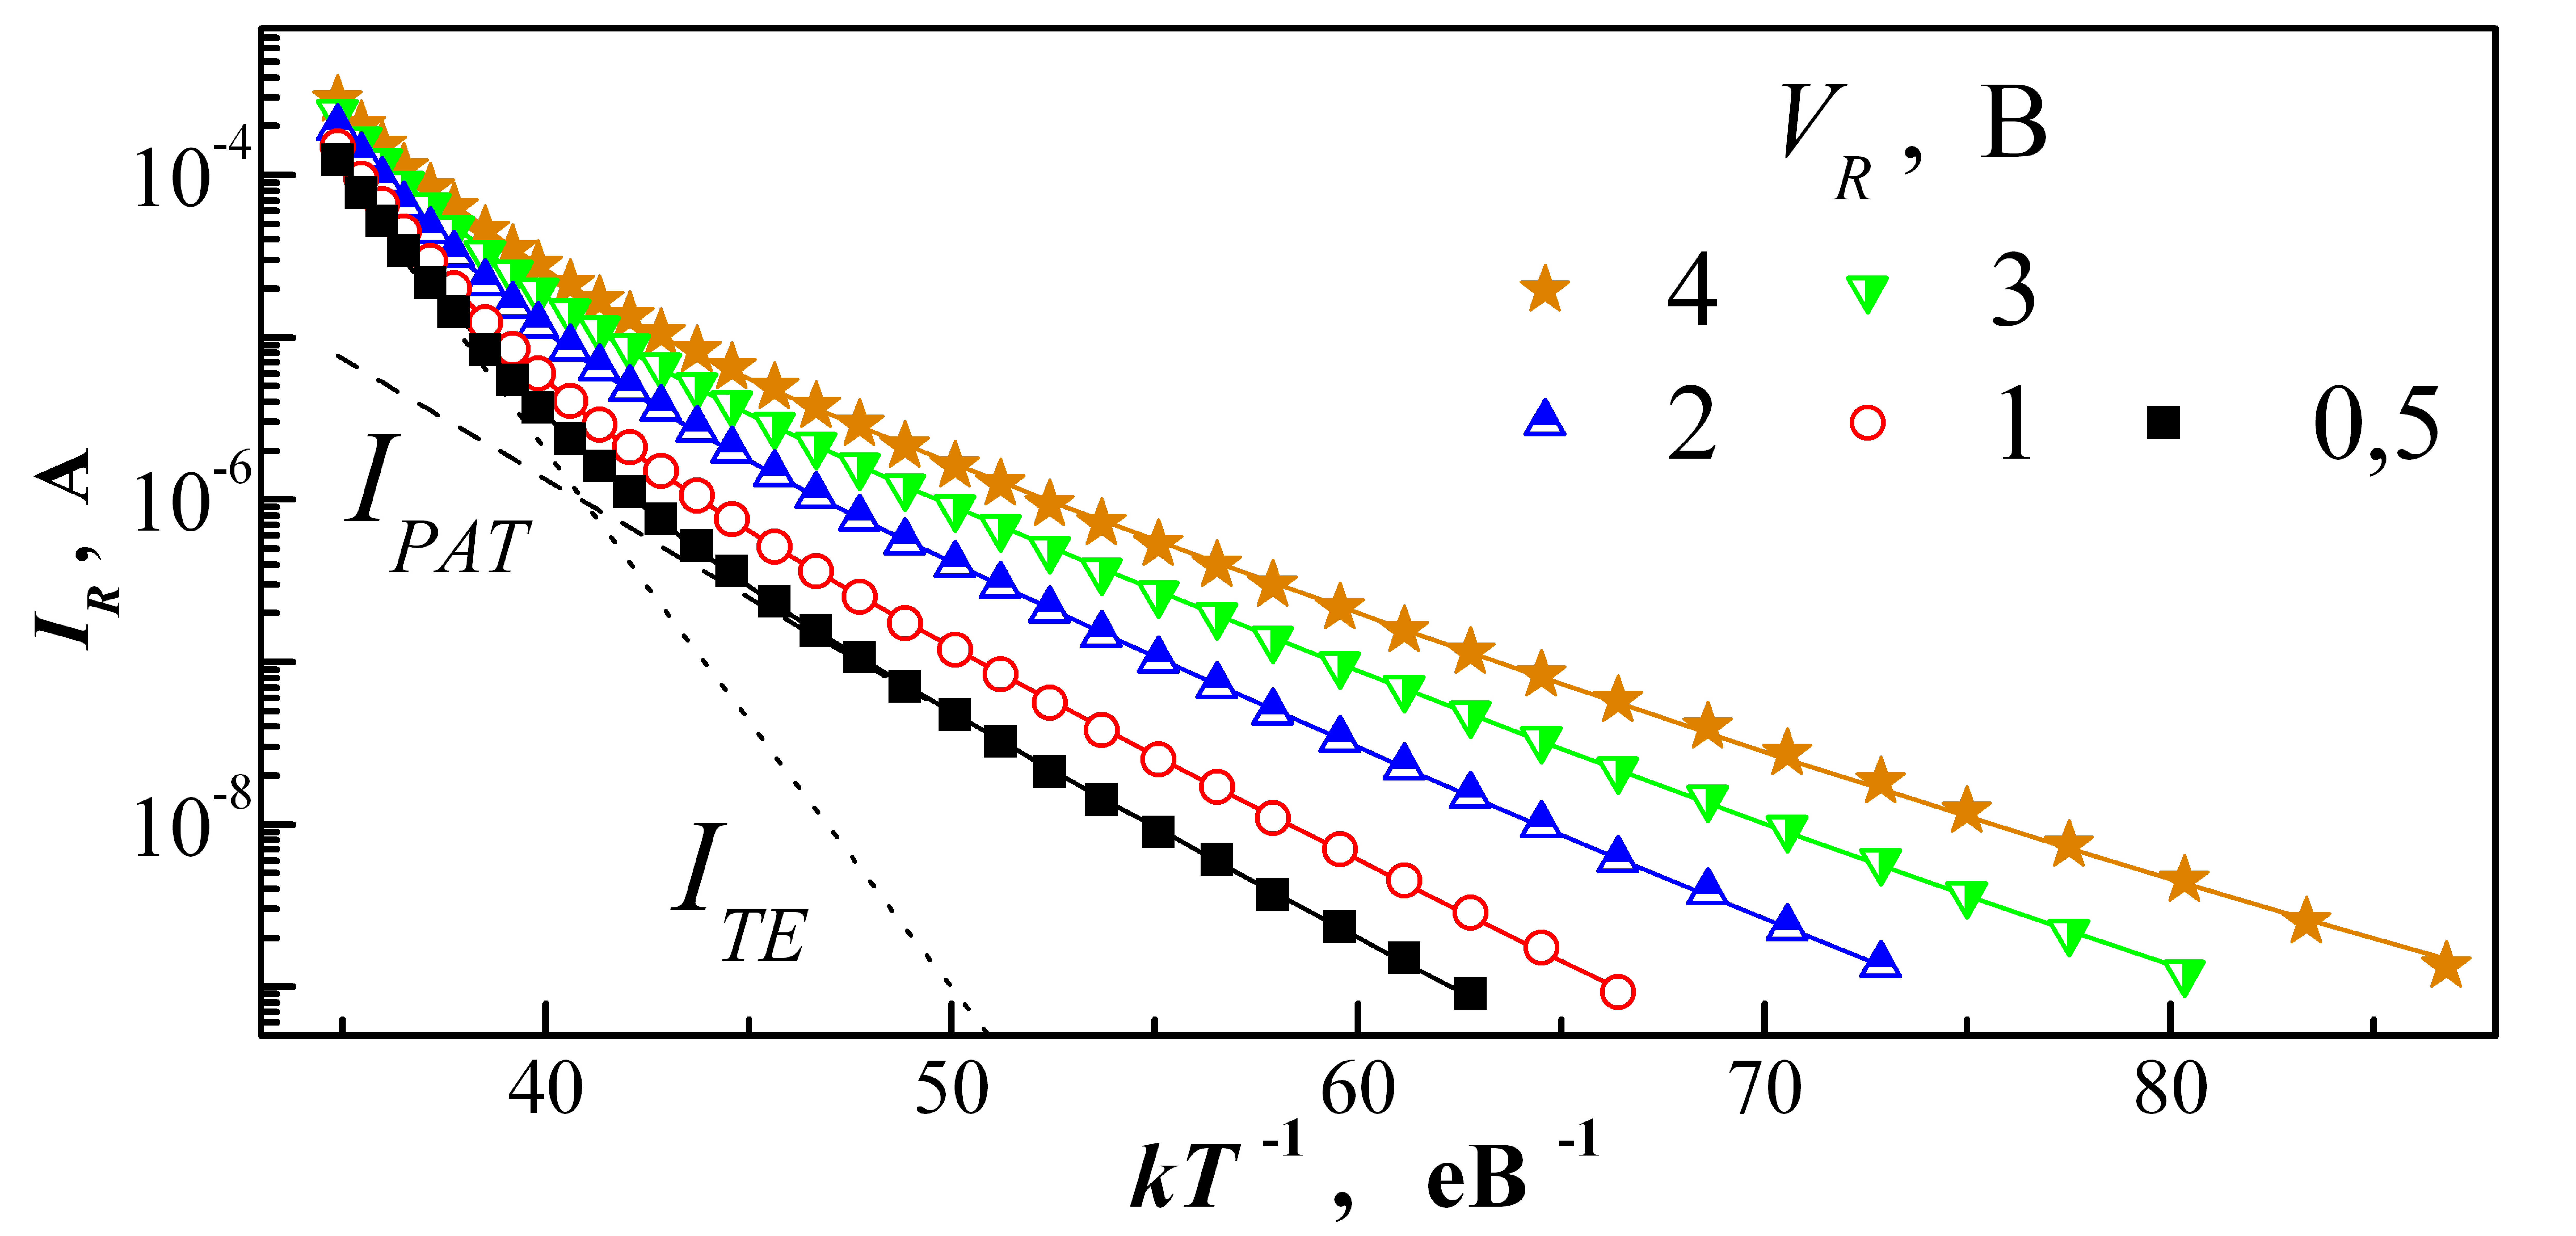
\includegraphics[width=0.7\textwidth]{figKT_SDB}
%\caption{\label{figKT_SDB}
%Залежності зворотного струму структур Mo$/n-n^+$--Si від оберненої температури,
%виміряні при різних напругах зміщення.
%Точки --- експеримент,
%суцільні лінії --- апроксимація відповідно до формули~(\ref{eqIgen}).
%Пунктирна та штрихована лінії відображають ТЕ та РАТ компоненти струму, відповідно
%}%
%\end{figure}


\begin{table}[hb]
\caption{Параметри, визначені для структур Mo$/n-n^+$--Si зі зворотних гілок ВАХ за умов УЗН та без нього}
\label{tabSDBParZv}
\centering
\begin{tabular}{|c|c|c|c|c|c|c|}
\hline
$W_\mathtt{US}$, &$f_\mathtt{US}$,&$\Phi_{b0}(0)$,&$\alpha_F$,&$\epsilon_{t0}$,&$\beta_F\cdot10^{5}$,&$N_{ss}$,\\
Вт/см$^2$&МГц&мВ&нм&меВ&еВ$\cdot$м$^{1/2}\cdot$В$^{-1/2}$&$10^{11}$см$^{-2}$\\\hline
0&---&$960\pm10$&$66\pm7$&$610\pm10$&$10,5\pm0,3$&$5,3\pm0,7$\\\hline
0,17&8,4&$870\pm10$&$51\pm5$&$540\pm10$&$\;\:8,1\pm0,5$&$1,2\pm0,2$\\\hline
0,65&4,1&$790\pm10$&$36\pm7$&$520\pm10$&$\;\:7,1\pm0,5$&$0,8\pm0,2$\\\hline
\end{tabular}
\end{table}

У  \underline{\textbf{шостому розділі}} представлені результати досліджень необоротних змін в структурах на основі арсеніду галію, викликаних мікрохвильовою (МХО) та ультразвуковою (УЗО) обробками,
а також акустовідпалу $\gamma$--опромінених кремнієвих структур метал--окис--напівпровідник (МОН).

Розглянуто вплив МХО (частота 2,45 ГГц, питома потужність  $1,5$~Вт/см$^2$, час обробки --- до 80~c) на параметри глибоких центрів, розташованих у приповерхневій області монокристалів $n$--6$H$--SiC та $n$--GaAs, а також арсенід галієвих епітаксійних структур за допомогою методу акустоелектричної релаксаційної спектроскопії.
Шляхом порівняння отриманих величин енергетичного положення рівнів з літературними даними проведено ідентифікацію відповідних дефектів у приповерхневому шарі монокристалів та на границі розділу епітаксійних структур.
Зокрема до опромінення виявлені комплекси вакансійного типу:
в $n$--6$H$--SiC V$_\text{Si}$V$_\text{C}$ (положення рівня $E_c-0,33$~еВ),
в $n$--GaAs V$_\text{As}$ ($E_c-0,32$~еВ) та V$_\text{Ga}$Ga$_i$V$_\text{As}$ ($E_c-0,49$~еВ),
в $n-n^+$--GaAs V$_\text{Ga}$V$_\text{As}$ ($E_c-0,24$~еВ), V$_\text{As}$As$_i$ ($E_c-(0,43-0,46)$~еВ) та V$_\text{Ga}$Ga$_\text{As}$ ($E_c-0,40$~еВ).
Внаслідок мікрохвильового опромінення біля поверхні збільшується концентрація міжвузольних атомів та відбуваються перетворення в дефектній
підсистемі внаслідок їх взаємодії з вихідними дефектами:
\begin{eqnarray*}
  \text{SiC}&:&\text{V}_\text{Si}\;\text{V}_\text{C}+\text{V}_\text{Si}\;\text{V}_\text{C}+\text{C}_{\,i}+ \text{C}_{\,i} \rightarrow \text{V}_\text{Si}+ \text{V}_\text{Si}\rightarrow \text{V}_\text{Si}\;\text{V}_\text{Si}\,;\\
  &&\text{V}_\text{Si}\;\text{V}_\text{Si}+\text{Si}_{\,i}+ \text{Si}_{\,i} \rightarrow 0\,;\\
  \text{GaAs}&:&\text{V}_\text{As}+ \text{As}_{\,i} \rightarrow\text{V}_\text{Si}\;\text{As}_{\,i} \rightarrow 0\,;\\
   &&  \text{V}_\text{Ga}\;\text{Ga}_{\,i}\;\text{V}_\text{As}\rightarrow \text{Ga}_\text{Ga}\;\text{V}_\text{As}
  \rightarrow \text{Ga}_\text{As}\;\text{V}_\text{Ga} \,;\\
  &&\text{V}_\text{Ga}\;\text{V}_\text{As}+\text{Ga}_{\,i}+\text{As}_{\,i} \rightarrow \text{V}_\text{As}\;\text{As}_{\,i}\,;\\
  &&  \text{V}_\text{Ga}\;\text{Ga}_\text{As}+\text{As}_{\,i} \rightarrow
  \text{Ga}_\text{Ga}\;\text{V}_\text{As}+\text{As}_{\,i} \rightarrow
  \text{V}_\text{As}\;\text{As}_{\,i}\,.
\end{eqnarray*}
Крім того, після МХО спостерігаються зміни (в декілька разів) поперечного перерізу захоплення електронів,
які пов'язані зі зміною напруженості електричного поля в околі дефектів.
Отримані результати щодо зміни параметрів дефектів корелюють з вимірами радіуса кривизни структур та деформації в приповерхневому шарі.
Зокрема, внаслідок МХО відбувається збільшення ступеню опуклості монокристалів, а наявність напруг сприяє радіаційно стимульованим дислокаційним реакціям.


Також досліджено вплив УЗО
($f_\mathtt{US}=(4,1\div30)$~МГц, $W_\mathtt{US}=(0,3\div3)$~Вт/м$^2$, час обробки $t_\mathtt{UST}=(5\div15)$~год) на параметри структур
Au--TiB$_x$--$n$--$n^+$--GaAs, виготовлених
по технології з інтегральним тепловідведенням (кожний зі зразків містив декілька десятків окремих діодів Шотткі).
Виявлено, що при $W_\mathtt{US}<2,5$~Вт/м$^2$ УЗО викликає зменшення розкиду ВБШ, фактора неідеальності та величини зворотного струму (рис.~\ref{figIrG_GA})
діодів Шотткі, виготовлених в єдиному технологічному процесі.
Ефект пов'язаний акусто--стимульованою дифузією точкових дефектів, яка призводить до згладжування локальних неоднорідностей границі розділу.
Зі збільшенням частоти УЗО інтенсифікуються процеси перебудови дефектів, що відображається у зміні характеристичного  параметра тунельної компоненти зворотного
струму.
При перевищенні інтенсивністю УЗО порогу ($(2,5\div3,0)$~Вт/м$^2$ спостерігається зменшення $\Phi_b$ та зростання $n_\mathrm{id}$ і зворотного струму внаслідок підсилення ТЕ складовою, що пов'язано з АІ генерацією дефектів.

\begin{figure}
\center
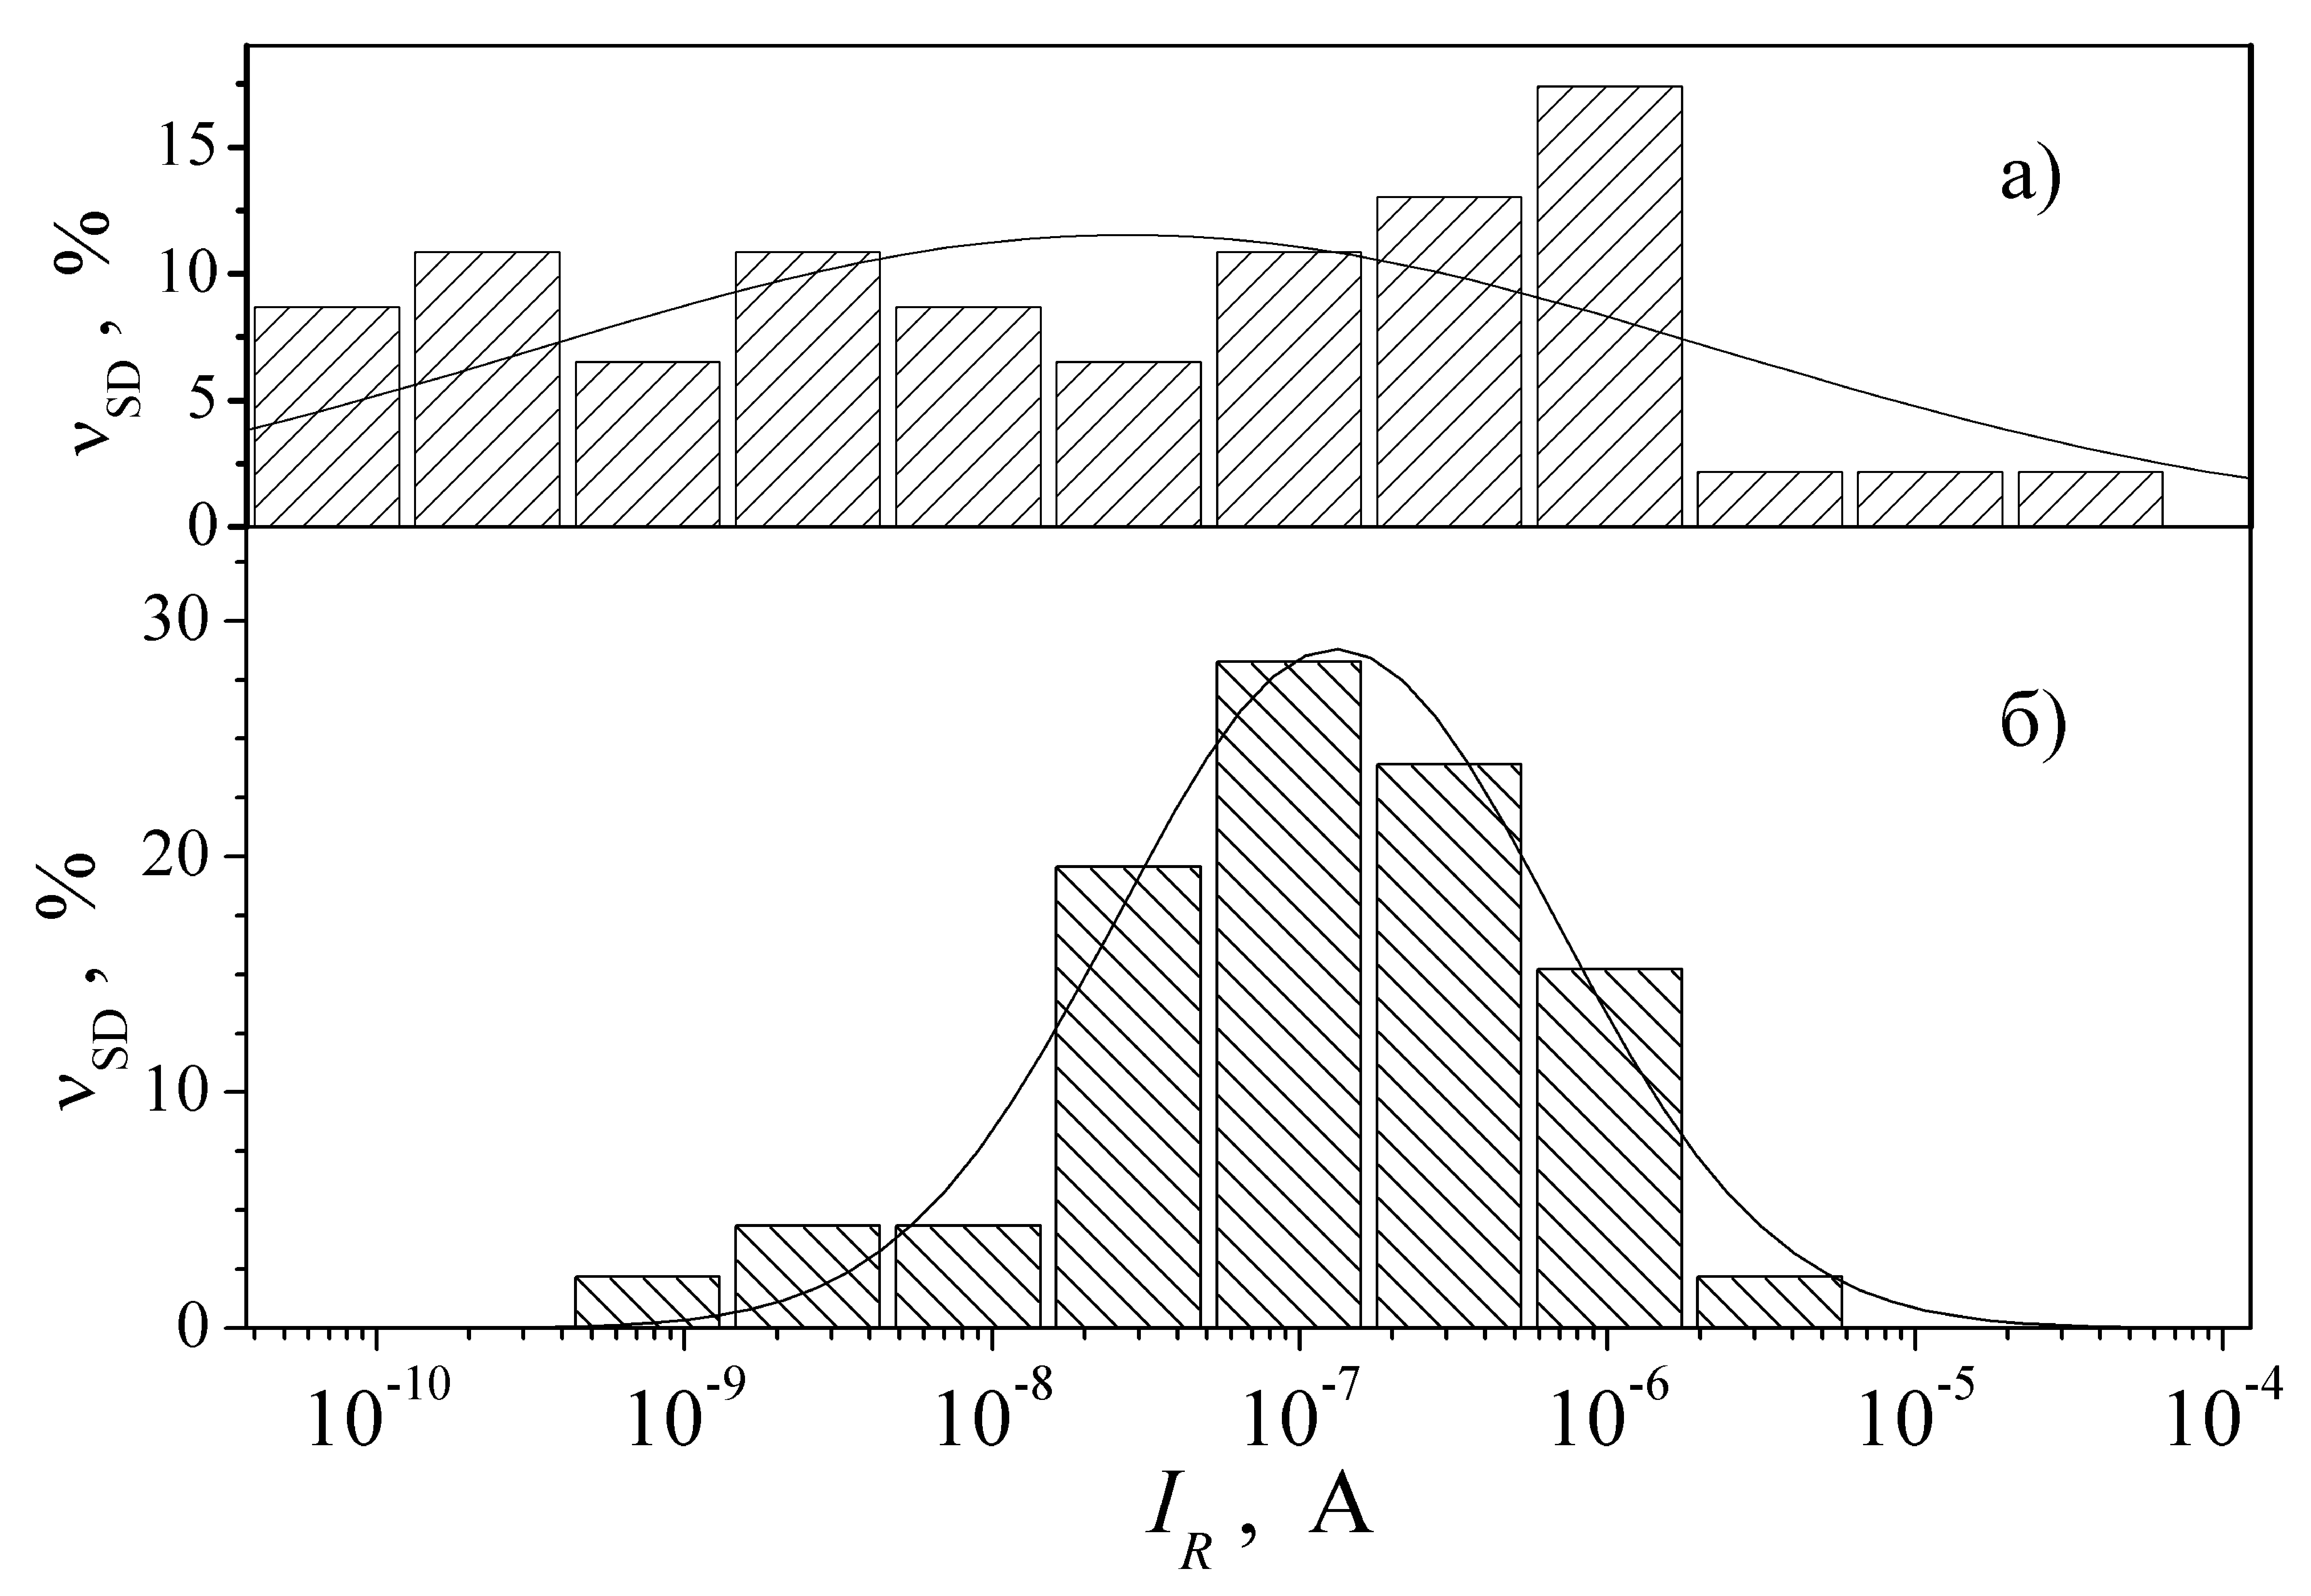
\includegraphics[width=0.7\textwidth]{figIrG_GA}%
\caption{\label{figIrG_GA}
Порівняльні розподіли величини зворотного струму (при $V_R=2$~В)
для структур Au--TiB$_x$--$n$--$n^+$--GaAs до УЗО (а) та після (б).
$W_\mathtt{US}=1,8$~Вт/см$^2$, $f_\mathtt{US}=4,1$~МГц, $t_\mathtt{UST}=10$~год.
По вертикалі відкладена частка діодів, для яких струм перебуває у відповідному діапазоні.
Загальна кількість діодів --- 40.
Лінії --- апроксимація відповідно до розподілу Гауса.
Середнє значення, А:
$(2,8\pm0,2)\cdot10^{-8}$ (а),
$(1,31\pm0,01)\cdot10^{-7}$ (б).
Дисперсія:
$9\pm2$ (а),
$3,3\pm0,2$ (б)
}
\end{figure}

\begin{figure}[b]
\center
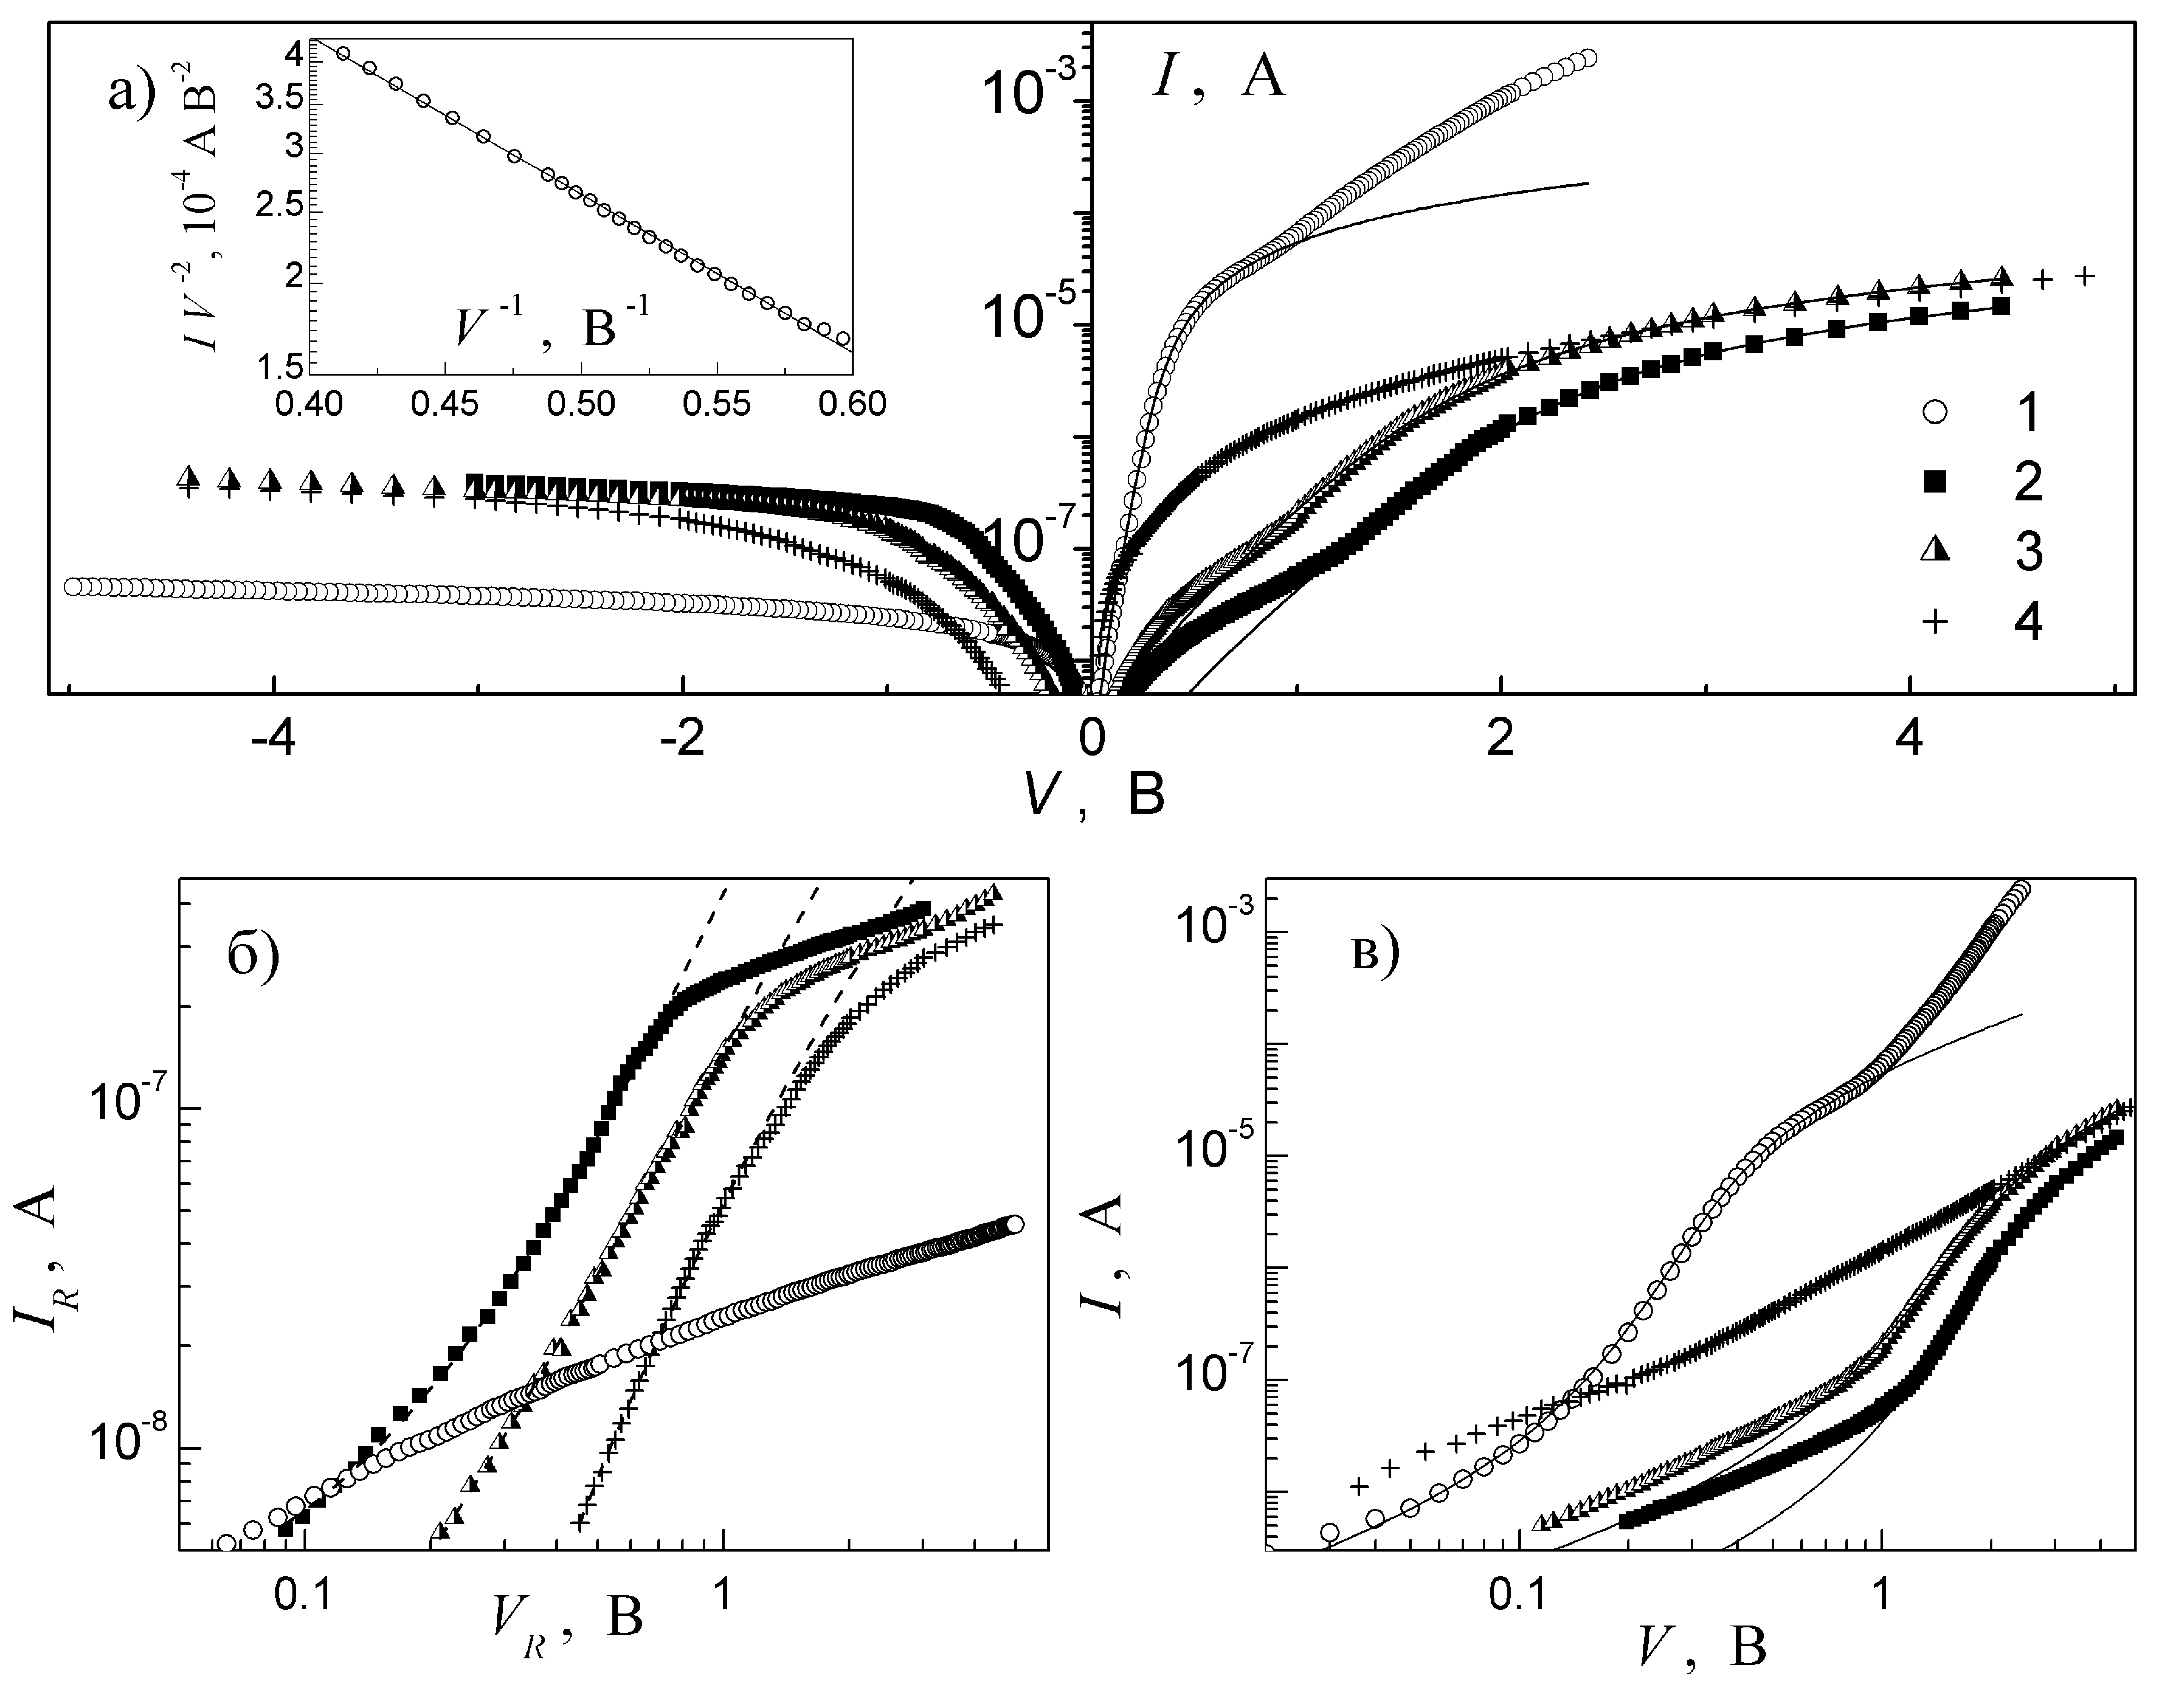
\includegraphics[width=0.85\textwidth]{figIV_MIS}%
\caption{\label{figIV_MIS}
Зворотні (а) та прямі (б) ВАХ структур Si--SiO$_2$--Au до (криві 1)
та після (2--4) опромінення $\gamma$--квантами.
$t_\mathtt{UST}$ , хв: 0 (2), 30 (3), 60 (4).
$T=300$~K.
Точки --- експеримент,
лінії --- апроксимація за формулами~(\ref{eqSDIV}) (суцільні) та (\ref{eqIVTAT}) (пунктир)
}%
\end{figure}
У шостому розділі також повідомляється про результати досліджень, спрямованих на з'ясування можливості відновлення характеристик Si--SiO$_2$--Au,
деградованих внаслідок $\gamma$--опромінення ($D=5\cdot10^7$~рад).
Виявлено, що використання подібних високих доз суттєво змінює процеси перенесення заряду в МОН--структурах --- рис.~\ref{figIV_MIS}.
Показано, що при малих прямих зміщеннях переважаючим стає струм, обмежений просторовим зарядом, для якого
\begin{equation}\label{eqVIsclc}
  I=I_0\,V^{\,m_\mathrm{F}},
\end{equation}
причому $I_0$ залежить від концентрації пасток $N_t$ ($I_0\sim 1/N_t^{m_\mathrm{F}-1}$),
диференційний показник ступеня $m_\mathrm{F}$ відображає енергетичний розподіл їх рівнів
%\cite{Jafar}
[10$^*$].
Поява даної компоненти струму пов'язана з утворенням ненасичених зв'язків на границі Si--SiO$_2$ ($P_b$--центрів).
Накопичення $P_b$--центрами від'ємного заряду на інтерфейсі також викликає зменшення ТЕ складової струму.
Опромінення також є причиною появи $E'$--центрів (вакансій кисню), що
викликає появу при зворотному зміщенні струму втрат, пов'язаного з тунелюванням по пасткам, для якого
\begin{equation}\label{eqIVTAT}
  I=I_{0,\mathrm{TAT}}\,(U_d+V_R)\exp\left(-\frac{R_\mathrm{TAT}}{F_m}\right),
\end{equation}
де параметр $I_{0,\mathrm{TAT}}$ пропорційний концентрації пасток.
УЗО
($f_\mathtt{US}=4$~МГц, $W_\mathtt{US}=2$~Вт/м$^2$, $t_\mathtt{UST}=(0,5\div1)$~год) викликає зменшення концентрації
$E'$--центрів ($I_{0,\mathrm{TAT}}$ зменшується в $\sim25$~разів) та  $P_b$--центрів ($I_0$ зростає в $\sim30$~разів),
а також звуження енергетичного спектра останніх ($m_\mathrm{F}$ змінюється з 1,3 до 1,8).
АІ ефекти пов'язані з акустостимульованою дифузію  атомів кисню та водню, причому ефективність пасивації останніми ненасичених зв'язків залежить
від рівня механічних напруг в околі дефекту.



%\newpage
%При использовании пакета \verb!biblatex! список публикаций автора по теме
%диссертации формируется в разделе <<\publications>>\ файла
%\verb!../common/characteristic.tex!  при помощи команды \verb!\nocite!
%
%\ifdefmacro{\microtypesetup}{\microtypesetup{protrusion=false}}{} % не рекомендуется применять пакет микротипографики к автоматически генерируемому списку литературы
%\ifnumequal{\value{bibliosel}}{0}{% Встроенная реализация с загрузкой файла через движок bibtex8
%  \renewcommand{\bibname}{\large \authorbibtitle}
%  \nocite{*}
%  \insertbiblioauthor           % Подключаем Bib-базы
%  %\insertbiblioother   % !!! bibtex не умеет работать с несколькими библиографиями !!!
%}{% Реализация пакетом biblatex через движок biber
%  \ifnumgreater{\value{usefootcite}}{0}{
%%  \nocite{*} % Невидимая цитата всех работ, позволит вывести все работы автора
%  \insertbiblioauthorcited      % Вывод процитированных в автореферате работ автора
%  }{
%  \insertbiblioauthor           % Вывод всех работ автора
%%  \insertbiblioauthorgrouped    % Вывод всех работ автора, сгруппированных по источникам
%%  \insertbiblioauthorimportant  % Вывод наиболее значимых работ автора (определяется в файле characteristic во второй section)
%  \insertbiblioother            % Вывод списка литературы, на которую ссылались в тексте автореферата
%  }
%}
%\ifdefmacro{\microtypesetup}{\microtypesetup{protrusion=true}}{}

      % Содержание автореферата


У  \underline{\textbf{другому розділі}} представлені результати експериментальних досліджень вперше виявлених оборотних акустоіндукованих (АІ) ефектів у радіаційно опромінених та неопромінених кремнієвих структурах з  $p$--$n$ переходом (сонячних елементах, КСЕ).

На початку представлені методики дослідження параметрів бар'єрних структур за умов ультразвукового навантаження (УЗН),
зокрема зосереджено увагу на схемі експерименту, яка унеможливлювала проникненню п'єзоелектричного поля у зразок (Рис.~\ref{USL_SC}), методи визначення параметрів АХ та режими УЗН.


\begin{figure}[ht]
\center
%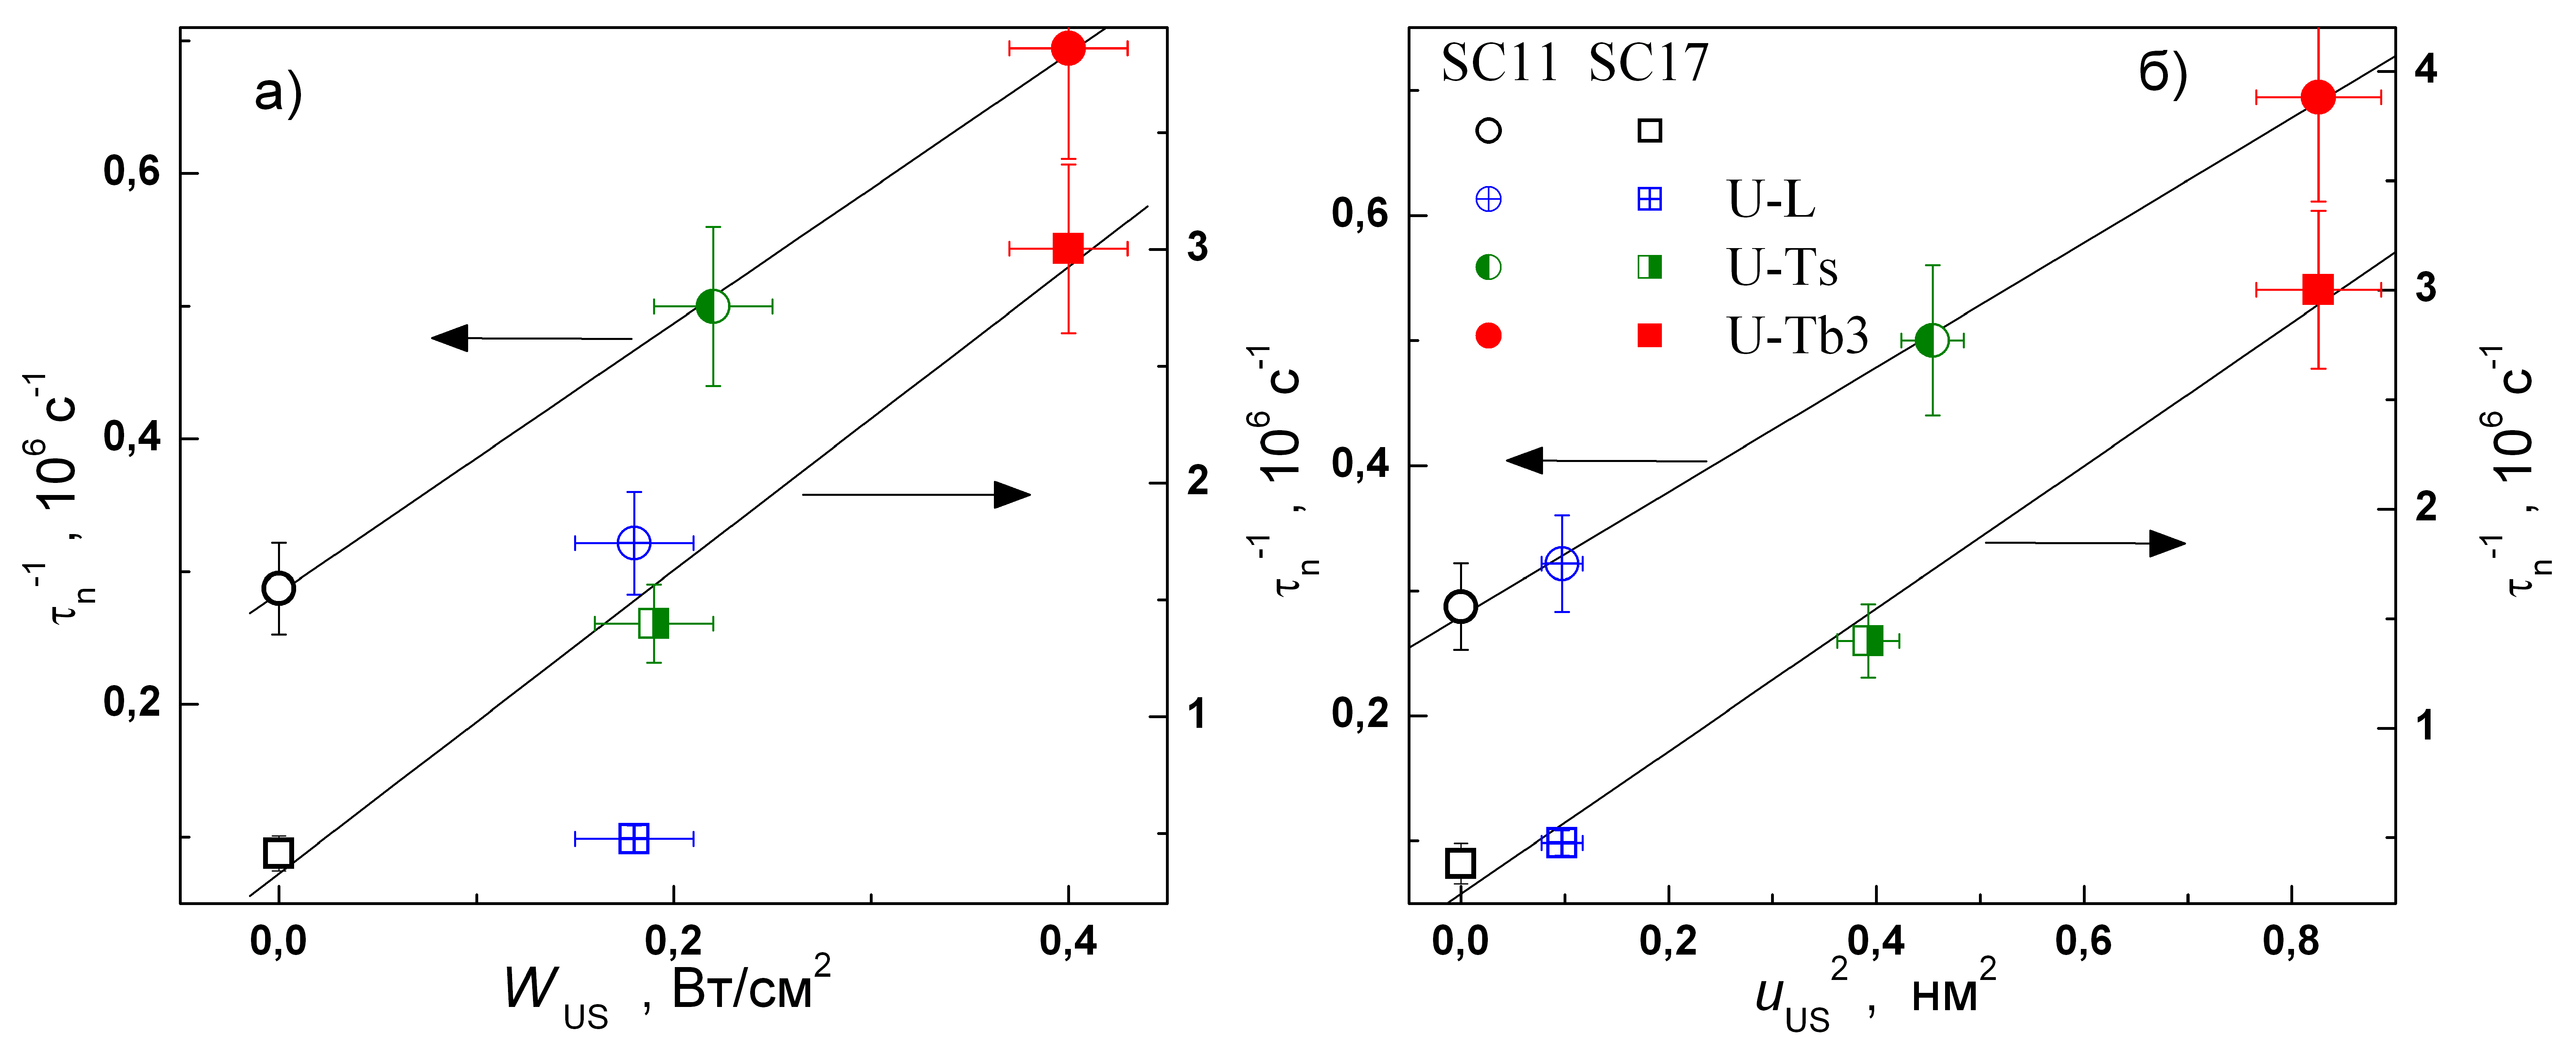
\includegraphics[width=1\textwidth]{figKus}%
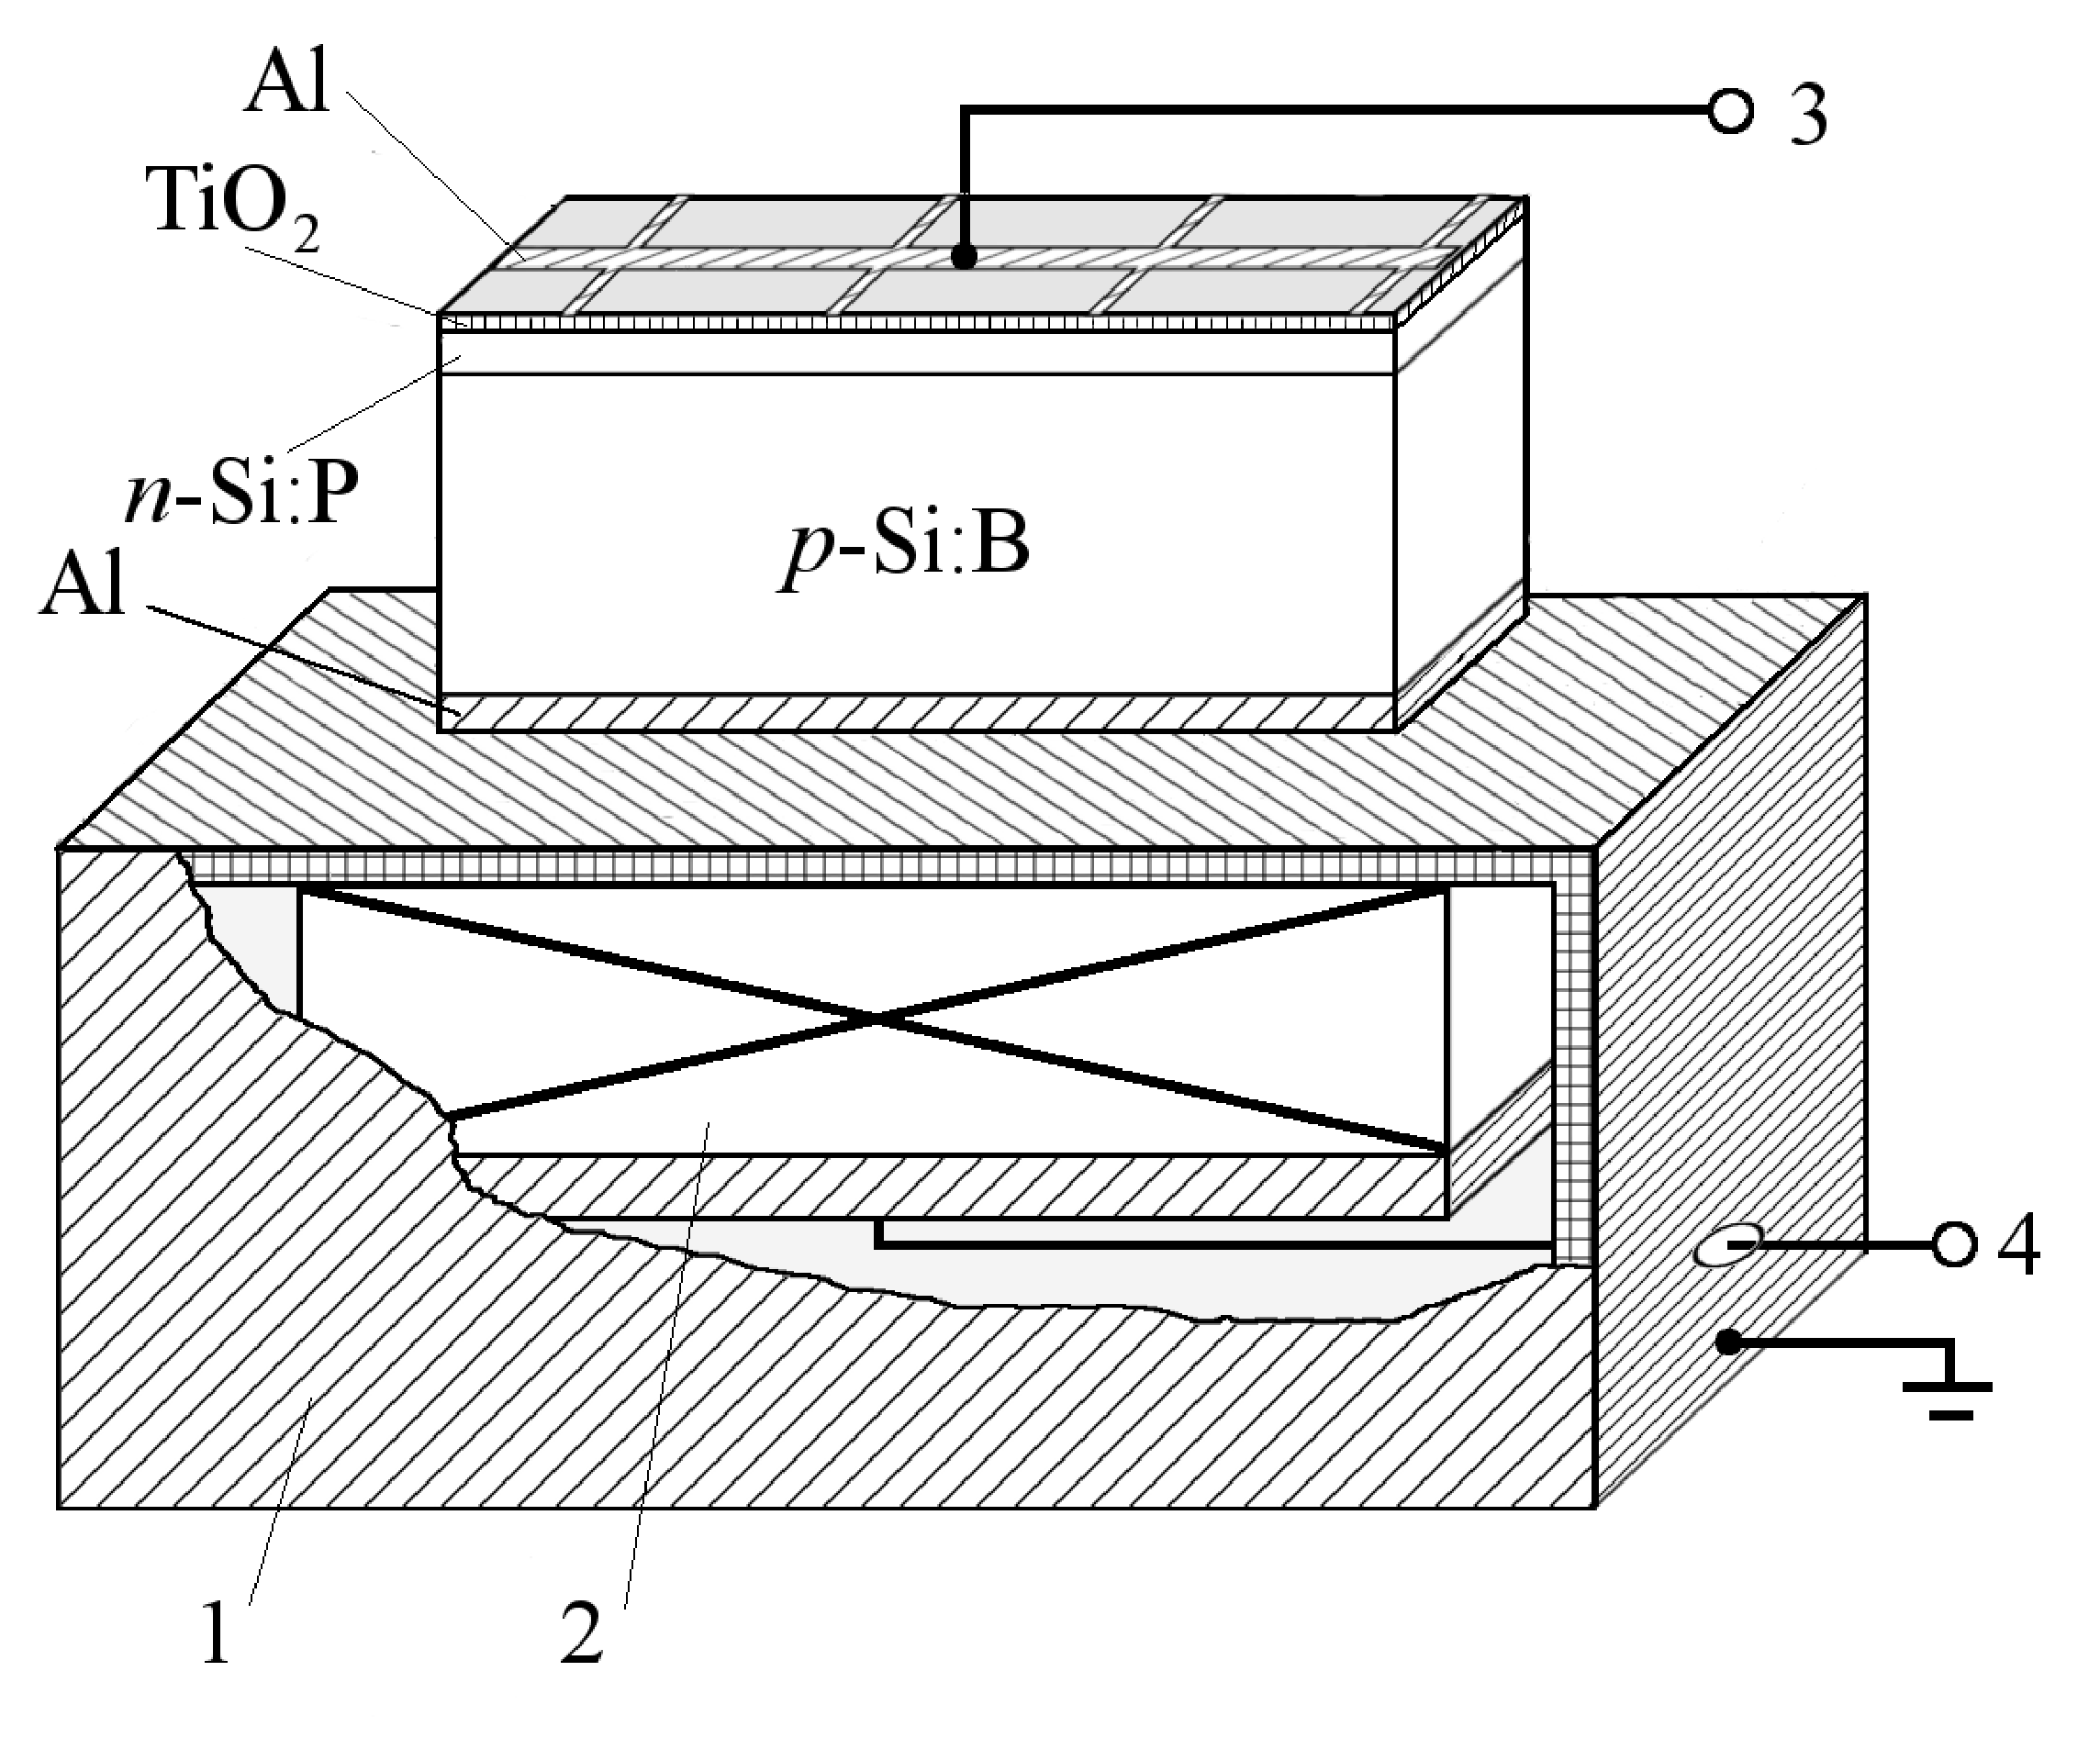
\includegraphics[width=0.4\textwidth]{USL_SC} \hfill
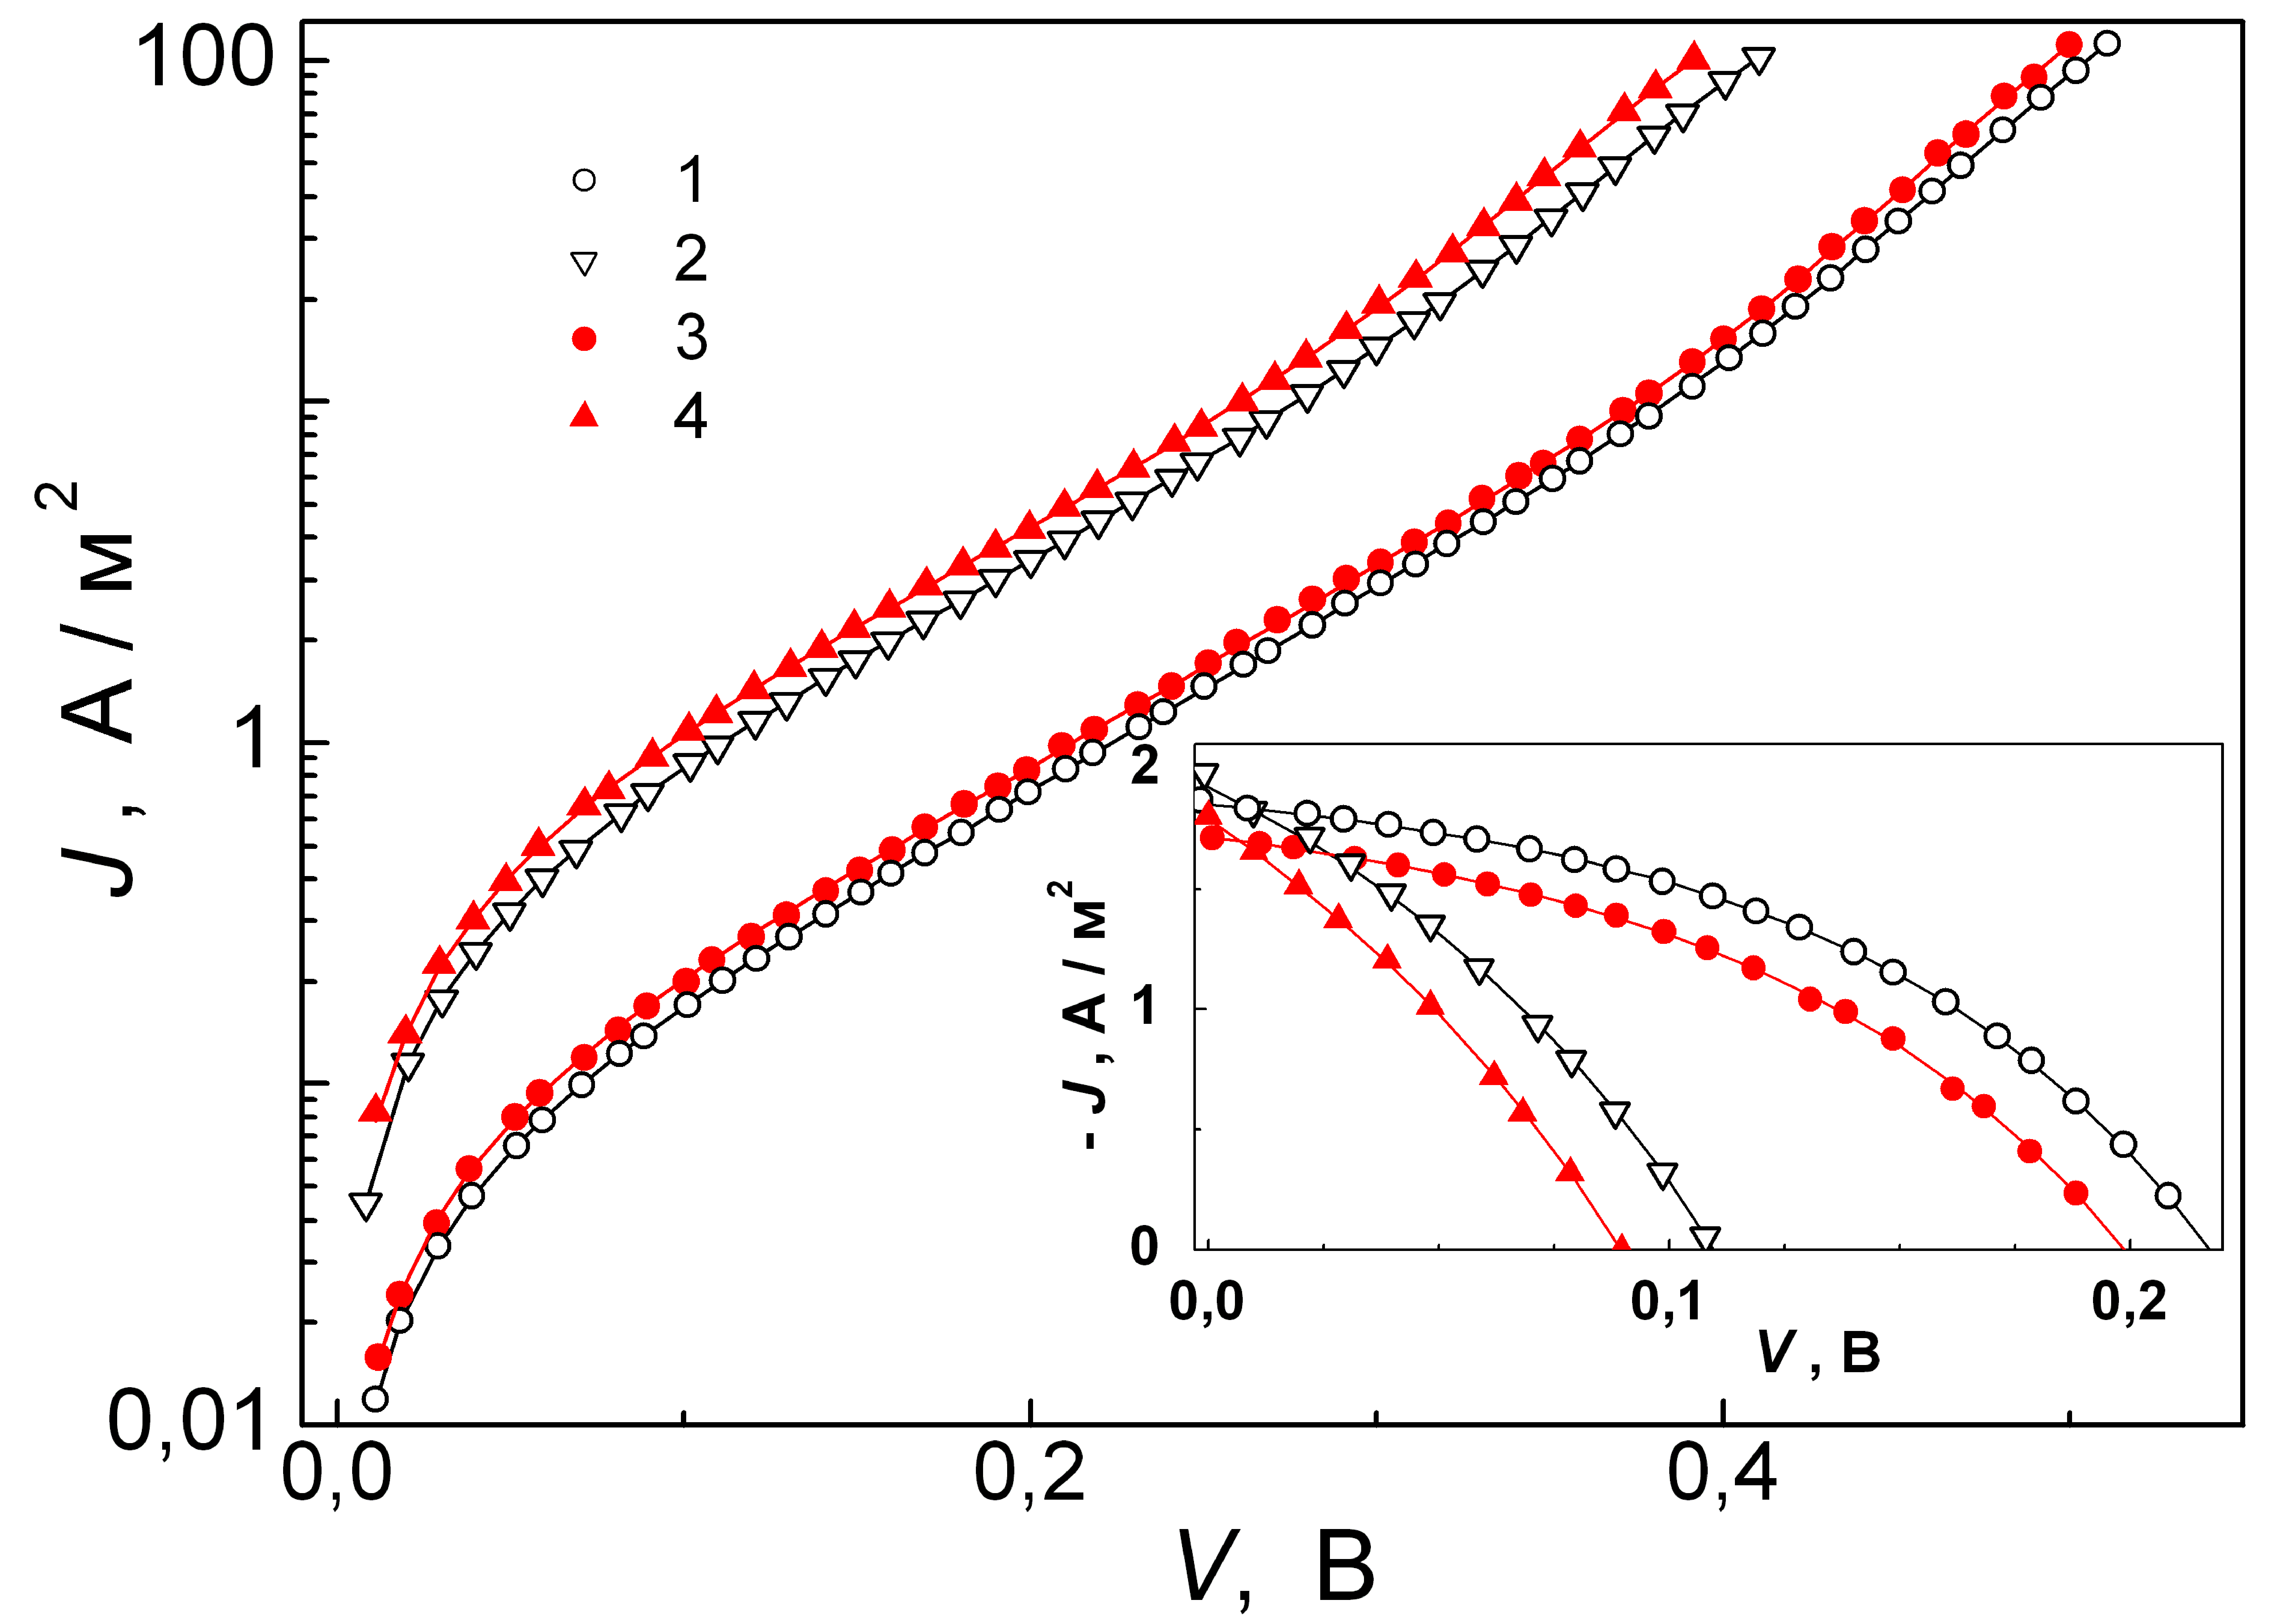
\includegraphics[width=0.55\textwidth]{figSSCIV}
\caption{\label{USL_SC}
Зліва --- схема УЗН.
1 --  екран (алюмінієва фольга, товщина 0,012 мм);
2 --- п'єзоелектричний перетворювач (LiNbO$_3$);
3 --- контакти для вимірювання ВАХ;
4 --- контакти для збудження УЗ.
Справа --- типові ВАХ, виміряні при температурах 301~K (криві 1 та 2, кола) та 341~K (2 та 4, трикутники)
за умов УЗН (2, 4, заповнені точки) та для ненавантаженого зразка (1 та 3, порожні точки)
Точки --- результати вимірів, лінії отримані шляхом апроксимації за формулою (\ref{eqSSCIV}).
}%
\end{figure}

Експериментально виявлено, що в діапазоні $290\div340$~К при поширенні УЗ в неопромінених КСЕ відбувається деградація
фотоелектричних властивостей: 
спостерігається зменшення густини струму короткого замикання $J_{sc}$ (до 10\%), напруги холостого ходу $V_{oc}$ (до 15\%) та фактори форми ВАХ $F\!F$ (до 5\%).
Зміни оборотні, значення параметрів  після припинення УЗН  та витримки зразків при кімнатній температурі протягом доби повертаються до своїх вихідних значень.
Величини АІ змін слабко залежать від температури, водночас при використанні поперечних АХ зменшення параметрів більш суттєві, ніж у випадку поширення в КСЕ повздовжніх хвиль тієї ж інтенсивності $W_\mathtt{US}$.
Останнє свідчить про те, що ефективність впливу УЗ визначається насамперед зміщеннями атомів (деформацією ґратки), а не загальною енергією коливань під час УЗН.


З метою встановлення фізичного механізму виявлених ефектів проведені дослідження поведінки електрофізичних параметрів КСЕ за умов УЗН.
Визначення параметрів проводилось шляхом апроксимації виміряних вольт--амперних характеристик (ВАХ) згідно з моделлю подвійного діоду:

\begin{eqnarray}
\label{eqSSCIV}
\nonumber J(V,\,T)&=&-J_{ph}+\frac{qn_id}{2\tau_{g}}\left\{\exp \left[\frac{q(V-JR_s)}{n_\mathrm{id}kT}\right]-1\right\}+\\
&&+\frac{qn_i^2}{p_p}\sqrt{\frac{\mu_nkT}{\tau_n}}\left\{\exp \left[\frac{q(V-JR_s)}{kT}\right]-1\right\}+\frac{V-JR_s}{R_{sh}}\,,
\end{eqnarray}
де
$J$ --- густина струму,
$V$ --- прикладена напруга,
$J_{ph}$ --- густина фотогенерованого струму,
$n_i$ --- концентрація власних носіїв заряду,
$\tau_{g}$  --- ефективний час життя носіїв заряду в області просторового заряду (ОПЗ),
$d$ --- товщина ОПЗ,
$p_p$ --- концентрація основних носіїв заряду в $p$--області,
%$E_g$ --- ширина забороненої зони напівпровідника,
%$N_c$ та $N_v$ --- ефективна густина станів поблизу дна зони провідності та вершини валентної зони, відповідно;
$n_\mathrm{id}$ --- фактор неідеальності
$R_s$ та $R_{sh}$ --- послідовний та шунтуючий опори, відповідно;
$\mu_n$ та $\tau_n$ --- рухливість та час життя неосновних носіїв в базі діоду.
При апроксимації з використанням методу диференційної еволюції (див. Рис.~\ref{USL_SC}) враховувались температурні та польові залежності $n_i$,
$d$, $\mu_n$, величини  $\tau_g$, $\tau_n$, $n_{\mathrm{id}}$, $R_{sh}$, $R_s$ та  $J_{ph}$ розглядалися як невідомі (шукані).
Крім того, оцінка $\tau_n$ проводилася по температурній залежності струму короткого замикання.

Величини $n_\mathrm{id}$ та $\tau_g$ пов'язані з рекомбінацією в ОПЗ.
Виявлені температурні залежності фактору неідеальності та часу життя в ОПЗ
($n_{\mathrm{id}}(T) \sim T_{\mathrm{id}}/T$,
$\tau_{g}(T)\sim\exp\left(-E_{\tau g}/kT\right)$,
де $T_{\mathrm{id}}$ та $E_{\tau g}$ певні характерні величини),
а також їх абсолютні значення ($n_{\mathrm{id}}>2$, $\tau_{g}\approx(10^{-8}\div10^{-7})$~c),
свідчать, що для опису процесів у досліджуваних структурах доцільно застосовувати модель рекомбінації в системі спарених рівнів двох окремих дефектів (CDLR, coupled defect level recombination) \cite{CDLR:JAP}.
УЗН викликає оборотне зростання $n_\mathrm{id}$  (до 0,04) та зменшення $\tau_g$ (до 30\%).
Оборотність АІ змін та незмінність $T_{\mathrm{id}}$ і $E_{\tau g}$ при поширенні АХ показують, що
при УЗН не відбуваються ні перебудова рекомбінаційних центрів (РЦ), ні зменшення їх концентрації.
Дослідження та оцінки показали, що рекомбінація в квазі--нейтральній області може бути описана в рамках моделі Шоклі--Ріда--Хола (SRH), при цьому $\tau_n^{-1}=\sum_i N_{d,i}\,\,\sigma_{n,i}\,\upsilon_{\mathrm{th},n}$
(де
кількість доданків в сумі визначається загальним числом різних РЦ,
кожен з яких характеризуються концентрацією $N_{d,i}$ та поперечним перерізом захоплення (ППЗ) електронів $\sigma_{n,i}$;
$\upsilon_{\mathrm{th},n}$ --- теплова швидкість електронів).
При УЗН спостерігається достатньо значне (до 90\%) зменшення $\tau_n$, причому
$\tau_{n}^{-1}\sim u_\mathtt{US}^2$ (де $u_\mathtt{US}$ --- амплітуда зміщень атомів при поширенні УЗ).

Було проведено дослідження впливу інтенсивного ($\sim2000$~Вт/м$^2$) довготривалого ($\sim15$~год) освітлення на параметри КСЕ.
Аналіз залишкових змін та перехідних процесів після припинення освітлення показав, що дефектами в ОПЗ та КНО, які приймають участь як у рекомбінаційних процесах, так у акусто--дефектнiй взаємодiї є, переважно, кисневмiснi преципiтати (КП).
Крім того, певний внесок у ці процеси пов'язаний з парами Fe$_i$B$_s$.

Для пояснення виявлених ефектів запропонована модель акустоактивного комплексного РЦ, який складається
з двох дефектів донорного та акцепторного типів (див. Рис.~\ref{fig_Model}) у випадку CDLR рекомбінації чи є точковим дефектом--комплексом з нееквівалентних компонент у випадку механізму SRH.
При поширенні УЗ на точковий дефект дії періодична сила, амплітуда якої залежить від зміни об'єму кристалу, що припадає на один дефект $\Delta\Omega_d$ \cite{MirzadeJAP2011}.
В рамках запропонованої моделі за умов УЗН компоненти РЦ здійснюють гармонічні коливання, частота та вісь яких визначаються акустичною хвилею, тоді як амплітуди та фази залежить також і від  $\Delta\Omega_d^\mathtt{D}$ та
$\Delta\Omega_d^\mathtt{A}$ кожної з них.
При цьому відстань між цими компонентами в умовах УЗН $r_\mathtt{US}$ залежить від часу

\begin{figure}[ht]
\center
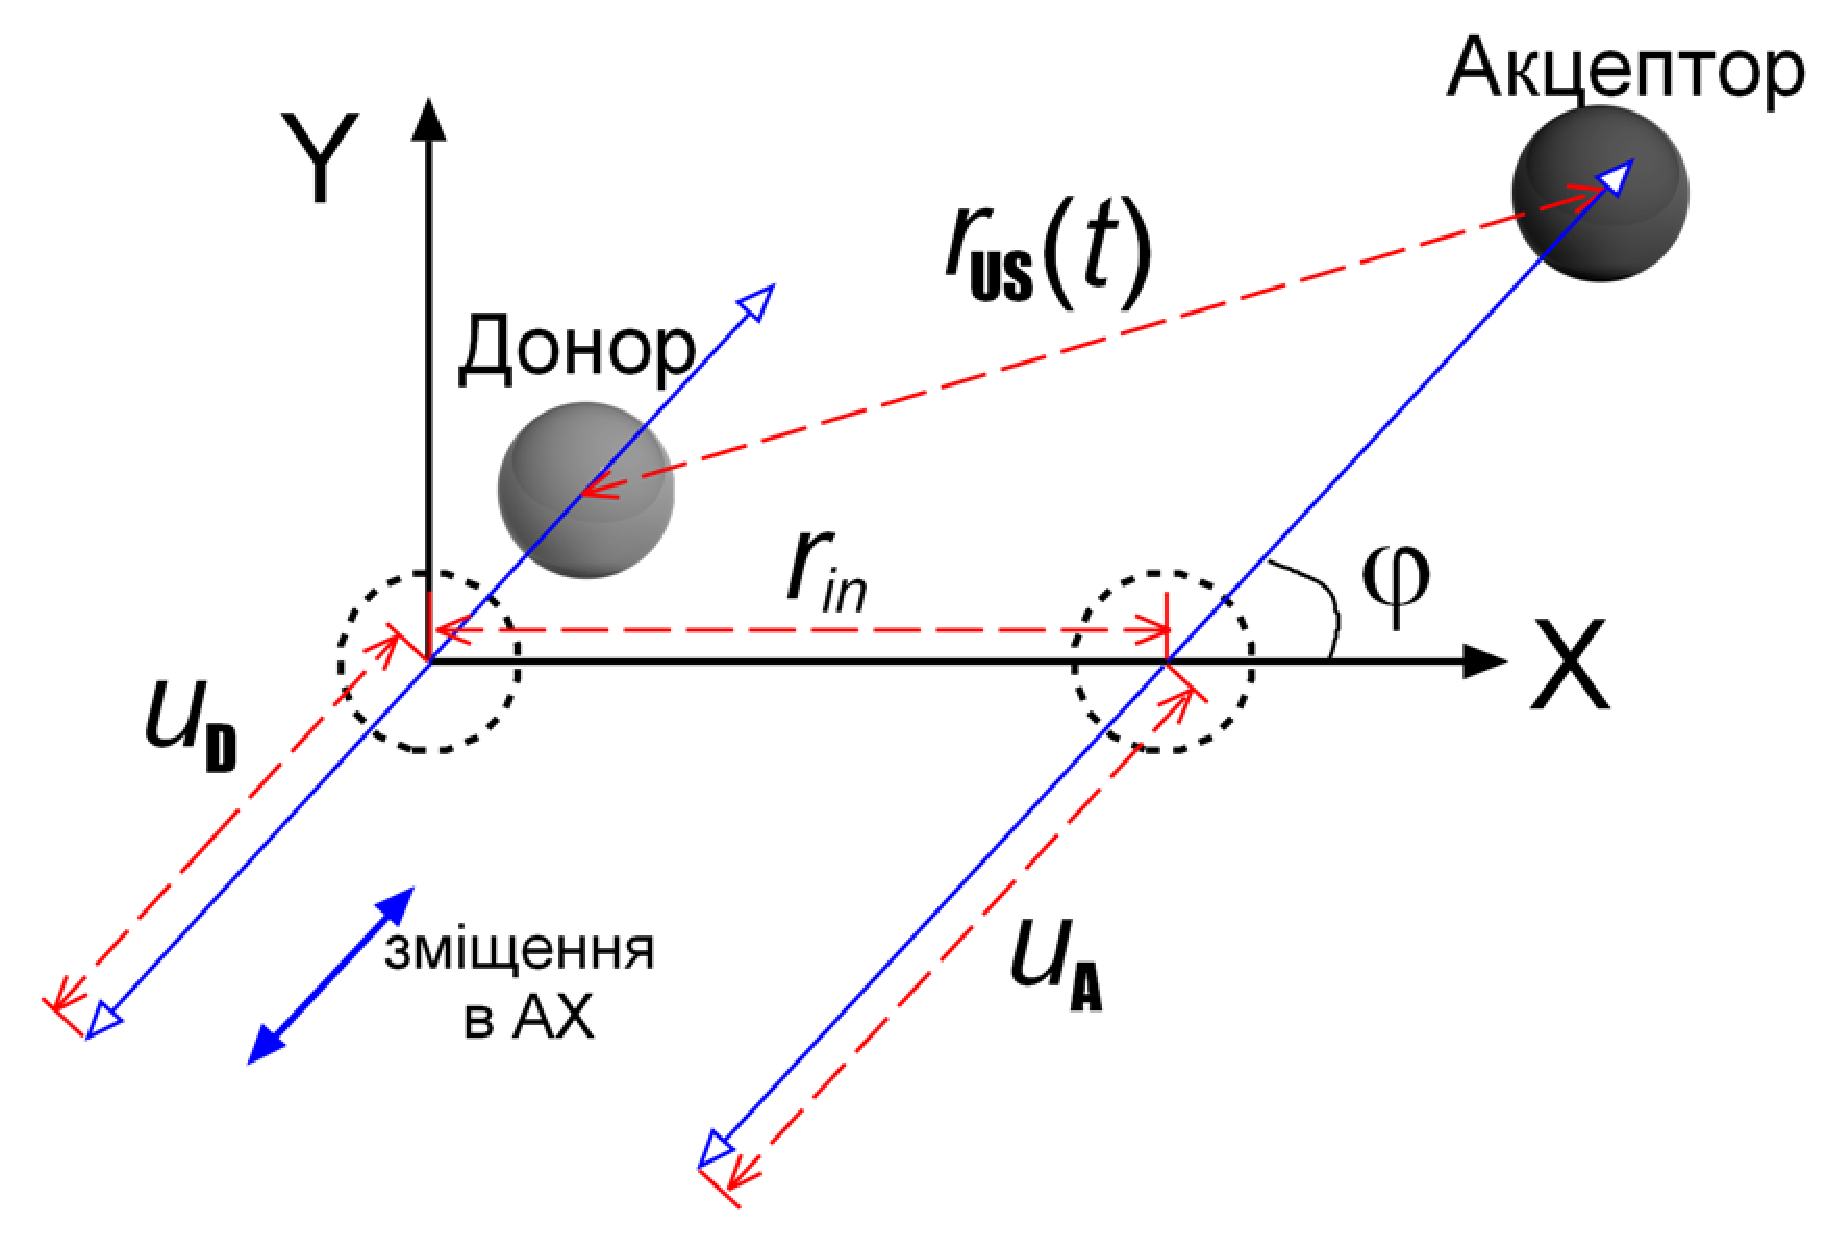
\includegraphics[width=0.5\textwidth]{fig_Model}
\caption{\label{fig_Model}
Модель поведінки дефектного комплексу в умовах УЗН.
}%
\end{figure}

\begin{multline}
\label{eqrUS}
r_\mathtt{US}(t)=\left\{[r_{in}+u_\mathtt{A}\cos(\omega_\mathtt{US}t+\delta)-u_\mathtt{D}\cos(\omega_\mathtt{US}t)]^2\cos^2\varphi \right.\\
    \left.+ [u_\mathtt{A}\cos(\omega_\mathtt{US}t+\delta)-u_\mathtt{D}\cos(\omega_\mathtt{US}t)]^2\sin^2\varphi\right\}^{0.5}\,,
\end{multline}
де
$r_{in}$ --- вихідна відстань,
$u_\mathtt{D}$ та $u_\mathtt{A}$ --- амплітуди коливань компонент, $u_\mathtt{D},\,u_\mathtt{A}\sim u_\mathtt{US}$,
$\omega_\mathtt{US}$ --- циклічна частота УЗ,
$\delta$ --- зсув фаз між коливаннями компонент,
$\varphi$ --- кут між віссю комплексу та напрямом зміщень в АХ.
В рамках запропонованої моделі були проведені розрахунки АІ змін $\sigma_{n}$ та так званого параметру зв'язку,
які визначають темп рекомбінації в наближеннях SRH та  CDLR.
Зокрема, 
а)~проведено аналіз ефективності УЗ впливу для різних РЦ при збудженні поперечних та повздовжніх АХ з врахуванням наявності просторово орієнтованих дислокацій та показано, що найбільші АІ зміни очікуються у випадку, коли комплекс складається з компонент міжвузольного та вакансійного типу в умовах поперечних коливань;
б)~збільшення ППЗ та зменшення параметру зв'язку має викликати зменшення $\tau_g$ та зростання $n_\mathrm{id}$, що спостерігається на експерименті;
в)~для часу життя в КНО за умов УЗН $\tau_{n,\mathtt{US}}$ справедливе співвідношення
\begin{equation}
\label{eqEpsSigUSA}
\tau_{n,\mathtt{US}}^{-1}=
\tau_{n,in}^{-1}+u_{\mathtt{US}}^2\,\sum_j\,N_{d,j}\,\sigma_{n,j}^{in}\,K_\mathtt{US,j}\,\upsilon_{\mathrm{th},n}\,,
\end{equation}
де
сумування здійснюється лише по акустоактивних (АА) РЦ,
$K_\mathtt{US,j}$ описує взаємодію УЗ з дефектом $j$--го типу.

Виявлено зменшення величини шунтуючого опору (до 30\%) при УЗН.
Спираючись на температурну залежність $R_{sh}$ показано, що його поява може бути описана в рамках моделі дислокаційно--індукованого імпедансу \cite{Rsh:Gopal2004}, а АІ зміни викликані зростанням ефективності захоплення електронів лінійними дефектами, розташованими в області $p$--$n$ переходу.

Проведені в рамках дводіодної моделі чисельні розрахунки показали, що АІ зміни $J_{sc}$ пов'язані зі зменшенням $\tau_{n}$,
тоді як зменшення $\tau_{g}$ викликає деградацію як $V_{oc}$, так i $F\!F$.
Ефект деградації підсилюється внаслідок АI зменшення $R_{sh}$ та частково компенсується зростанням $n_\mathrm{id}$.

Додатково, за допомогою методу диференційним коефіцієнтів ВАХ \cite{Bulyar}, проведено аналіз впливу УЗН на параметри дефектів в ОПЗ неопромінених КСЕ.
Шляхом детального аналізу літературних даних проведена ідентифікація дефектів, пов'язаних з виявленими енергетичними рівнями.
А саме, основними дефектами є КП ($E_c-(0,46\div0,48)$~еВ та $E_c-0,40$~еВ), дислокації ($E_c-0,36$~еВ) та комплекси Fe$_i$O$_i$ ($E_c-0,36$~еВ).
При УЗН відбувається незначне (близько 0,01~еВ) зменшення енергії активації та збільшується внесок
у рекомбінацію більш мілких рівнів, зокрема КП, причому зміни відносних внесків різних центрів практично лінійно залежать від $u_\mathtt{US}$.

Також представлені результати аналізу ВАХ, виміряних за умов УЗН та без нього, для КСЕ опромінених $\gamma$--квантами $^{60}$Co (дози $10^6$ та $10^7$~рад) та реакторними нейтронами (флюєнс $4\cdot10^{11}$~см$^{-2}$).
Виявлено,


\begin{figure}[ht]
\center
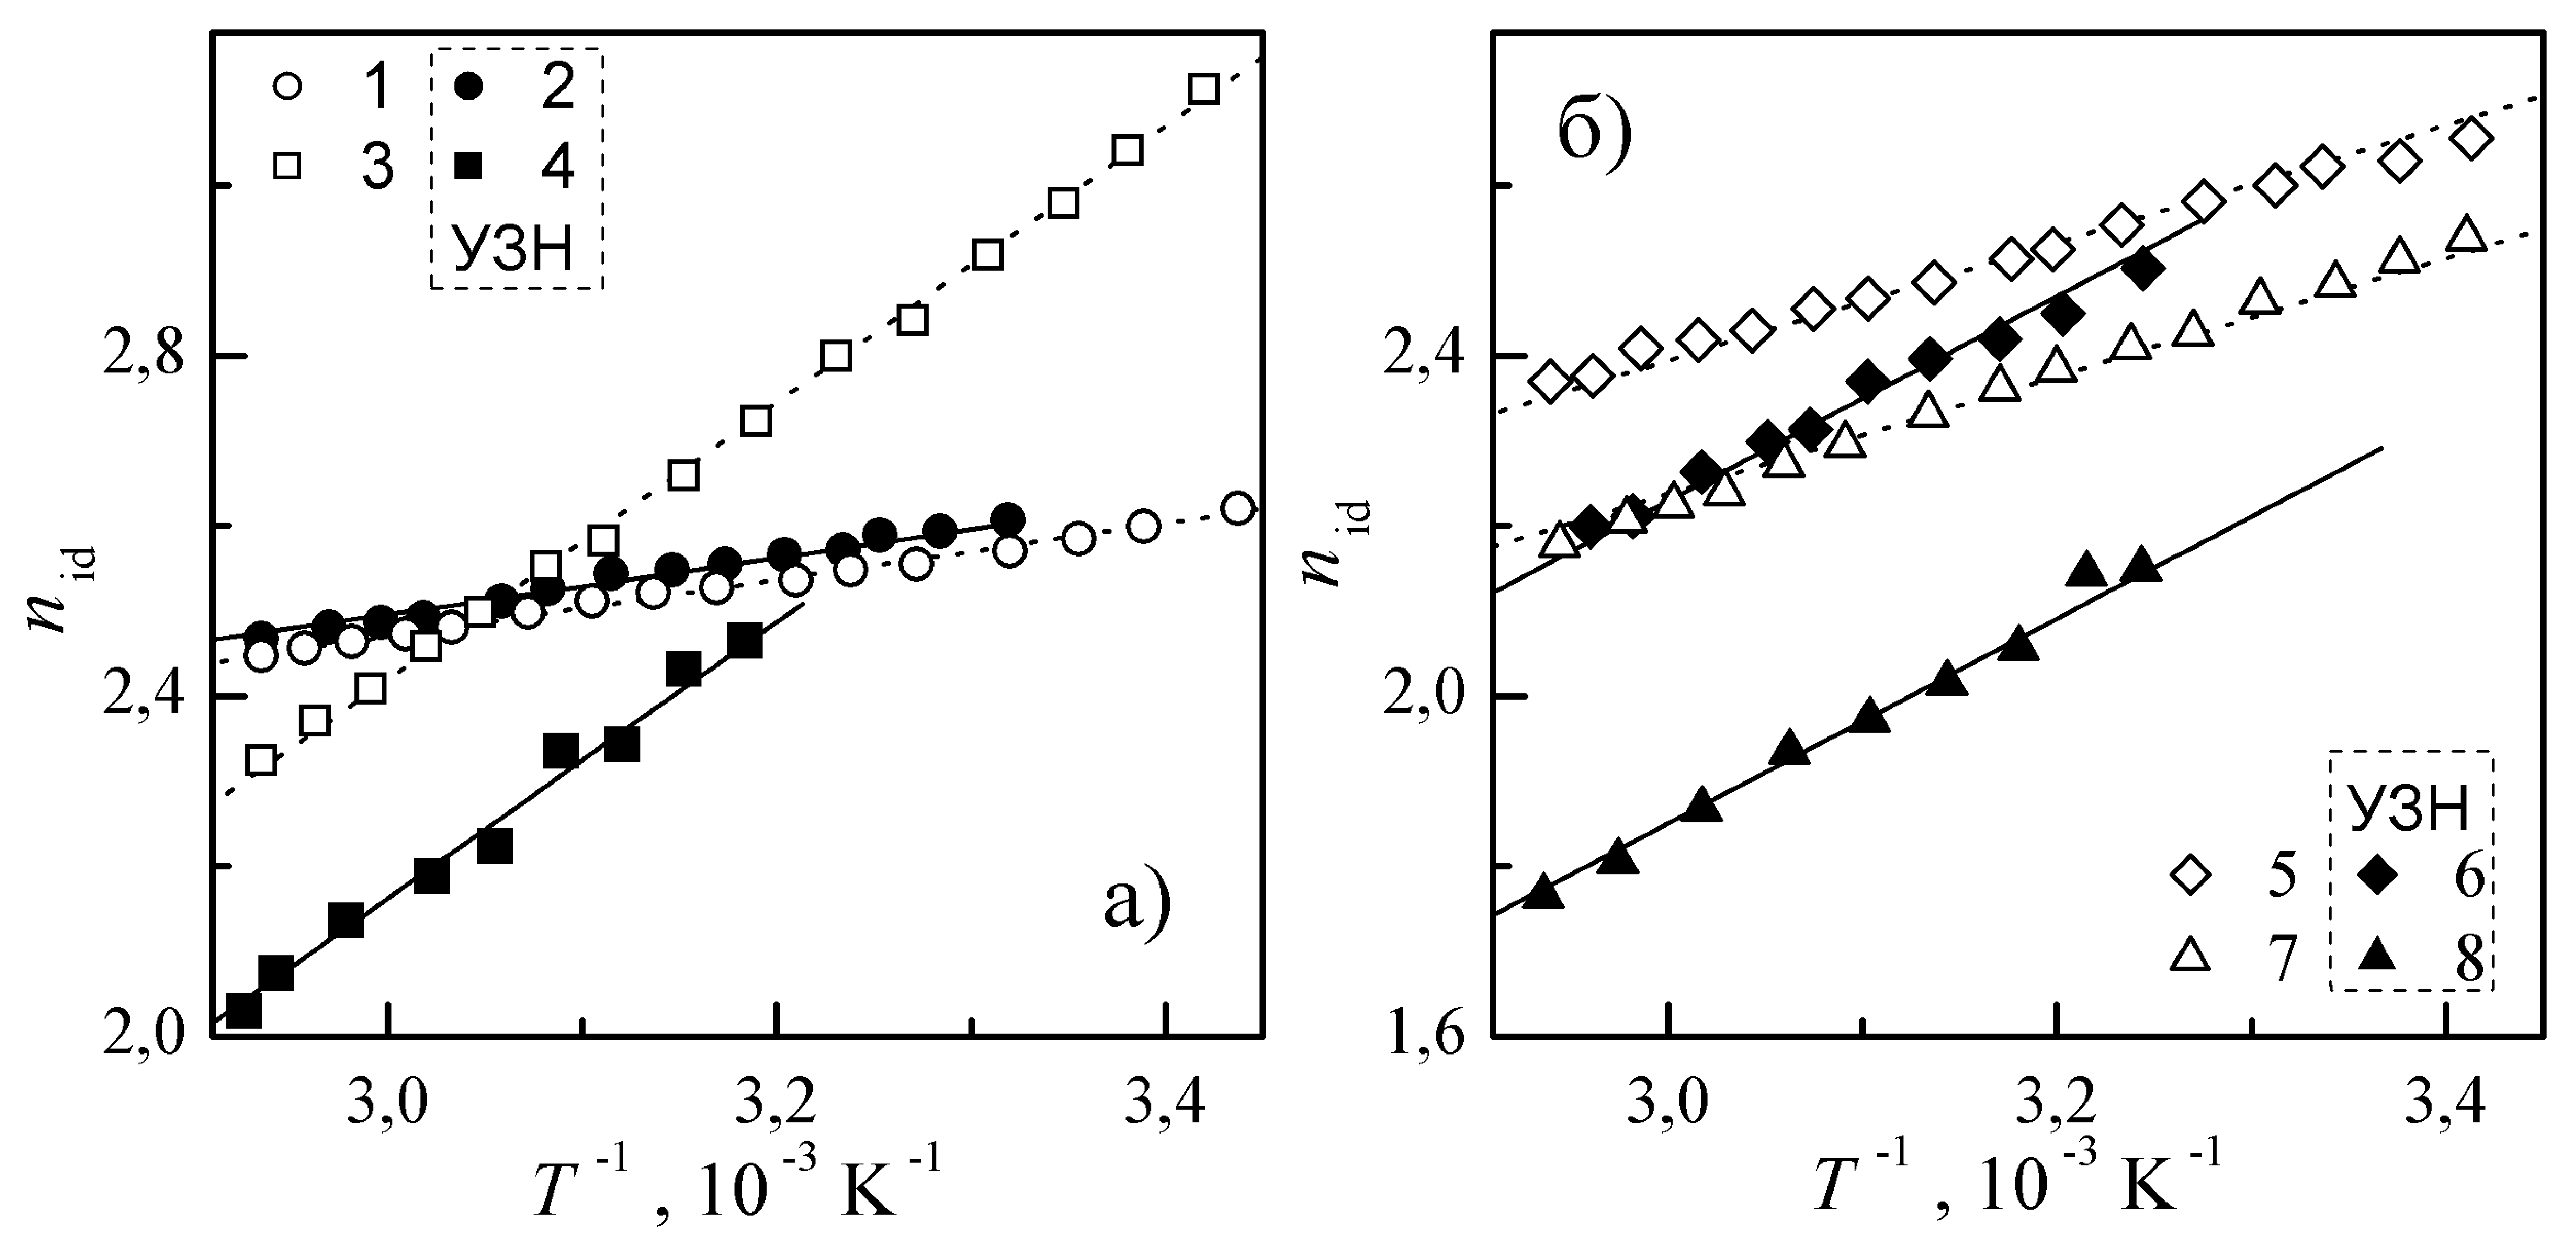
\includegraphics[width=0.9\textwidth]{fignRD}%
\caption{\label{fignRD}
Температурні залежності фактору неідеальності
для неопроміненого (криві 1, 2),
нейтронно--опроміненого (3, 4) та
гамма--опромінених (5, 6 та 7, 8 для доз $10^6$ та $10^7$~рад, відповідно)
зразків.
Криві 1, 3, 5 та 6 отримані без УЗН,
криві 2, 4, 9 та 8 відповідають УЗН (поперечні хвилі, 4,2~МГц, 0,4~Вт/см$^2$).
}%
\end{figure}


\begin{figure}[ht]
\center
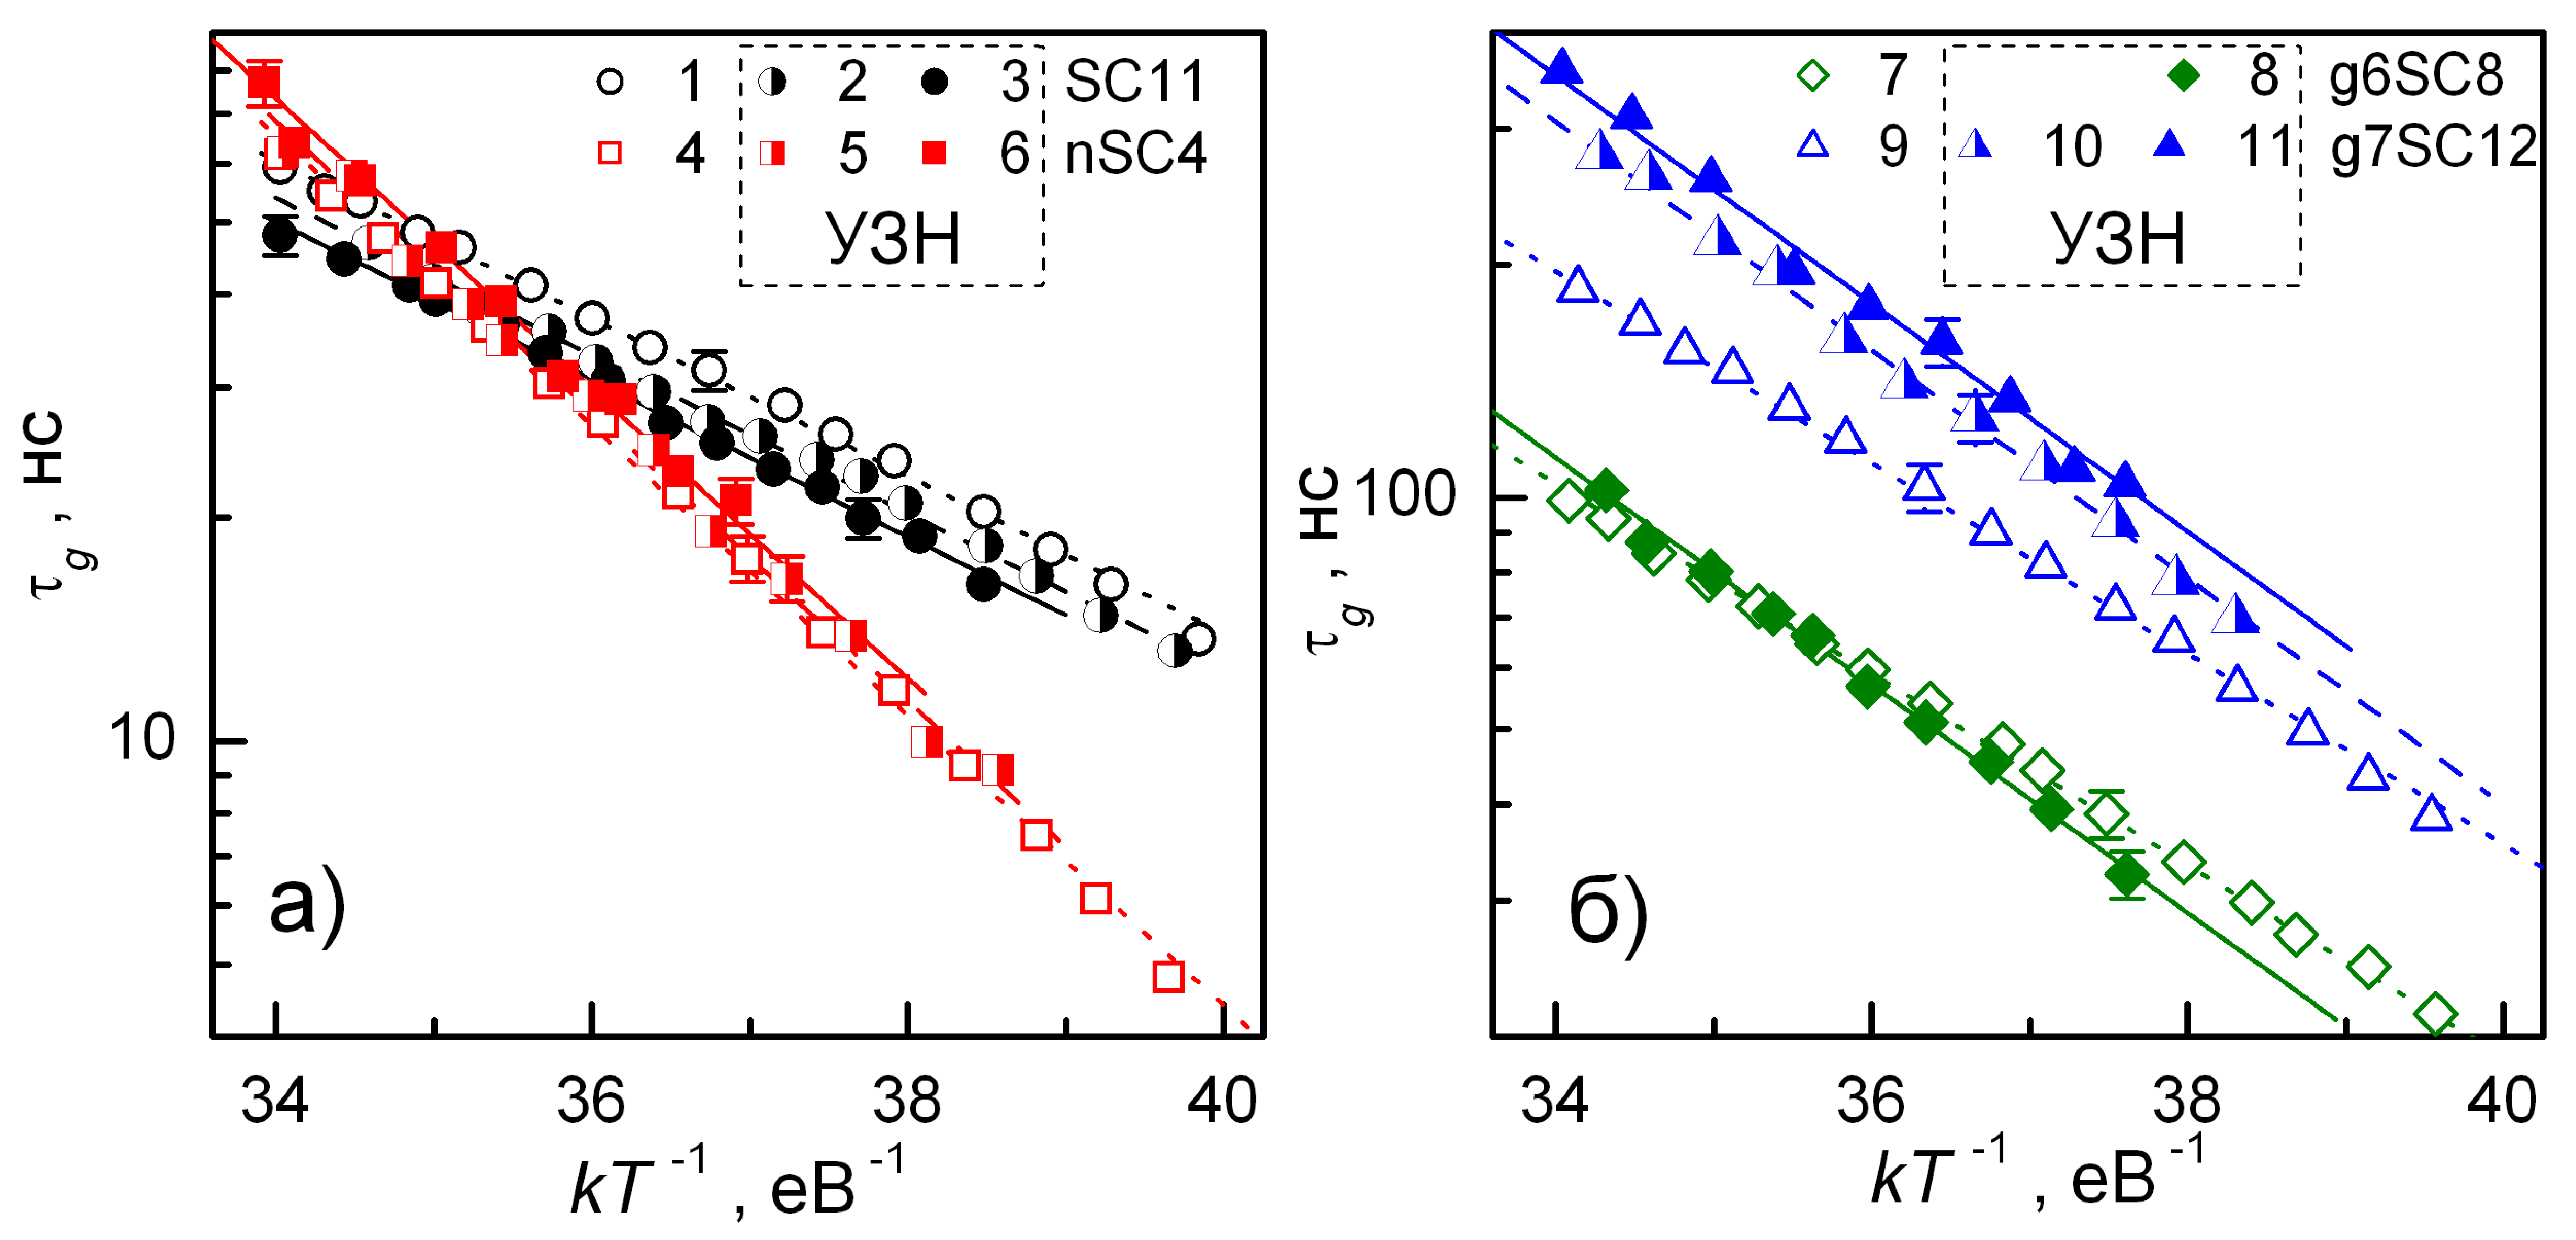
\includegraphics[width=0.9\textwidth]{figTAUgRD}%
\caption{\label{figTAUgRD}
Температурні залежності $\tau_g$.
Позначення кривих збігаються з Рис.~\ref{fignRD}.
}%
\end{figure}


Наведені   результати  підтверджують  практичну перспективність динамічного акустичного керування характеристиками напівровідникових приладів. 
Підкреслимо, що нерівноважний стан дефектів, який виникає при появі нерівноважних носіїв при проходженні струму, є важливим фактором підвищення ефективності акусто--дефектної взаємодії.

У  \underline{\textbf{третьому розділі}} представлені результати досліджень


У  \underline{\textbf{четвертому розділі}} представлені результати досліджень


У  \underline{\textbf{п'ятому розділі}} представлені результати досліджень


У  \underline{\textbf{шостому розділі}} представлені результати досліджень


Во \underline{\textbf{введении}} обосновывается актуальность
исследований, проводимых в~рамках данной диссертационной работы,
приводится обзор научной литературы по изучаемой проблеме,
формулируется цель, ставятся задачи работы, излагается научная новизна
и практическая значимость представляемой работы. В~последующих главах
сначала описывается общий принцип, позволяющий ..., а~потом идёт
апробация на частных примерах: ...  и~... .


\underline{\textbf{Первая глава}} посвящена ...

 картинку можно добавить так:
\begin{figure}[ht]
  \centering
  \includegraphics [scale=0.27] {latex}
  \caption{Подпись к картинке.}
  \label{img:latex}
\end{figure}

Формулы в строку без номера добавляются так:
\[
  \lambda_{T_s} = K_x\frac{d{x}}{d{T_s}}, \qquad
  \lambda_{q_s} = K_x\frac{d{x}}{d{q_s}},
\]

\underline{\textbf{Вторая глава}} посвящена исследованию

\underline{\textbf{Третья глава}} посвящена исследованию

Можно сослаться на свои работы в автореферате. Для этого в файле
\verb!Synopsis/setup.tex! необходимо присвоить положительное значение
счётчику \verb!\setcounter{usefootcite}{1}!. В таком случае ссылки на
работы других авторов будут подстрочными.
\ifnumgreater{\value{usefootcite}}{0}{
Изложенные в третьей главе результаты опубликованы в~\cite{vakbib1, vakbib2}.
}{}
Использование подстрочных ссылок внутри таблиц может вызывать проблемы.

В \underline{\textbf{четвертой главе}} приведено описание








Основні результати представленої роботи полягають у наступному.
%% Согласно ГОСТ Р 7.0.11-2011:
%% 5.3.3 В заключении диссертации излагают итоги выполненного исследования, рекомендации, перспективы дальнейшей разработки темы.
%% 9.2.3 В заключении автореферата диссертации излагают итоги данного исследования, рекомендации и перспективы дальнейшей разработки темы.
\begin{enumerate}[leftmargin=0cm,itemindent=3em]
  \item Вперше експериментально досліджено вплив ультразвукового навантаження на параметри монокристалічних кремнієвих сонячних елементів у діапазоні температур 290$\div$340~К
  та виявлено оборотну акусто--індуковану деградацію фотоелектричних властивостей, зумовлену зменшенням часу життя носіїв заряду в акустичному полі.
  Виявлено, що в умовах акустичного навантаження збільшується внесок у рекомбінаційні процеси мілкіших рівнів.
  Встановлено, що кисневмісні преципітати ефективно впливають на процеси рекомбінації та беруть участь у акусто--дефектній взаємодії.
  Запропоновано модель акустоактивного комплексного дефекту для пояснення особливостей акусто--індукованих ефектів.
 Виявлено ефект акусто--індукованого зменшення  опору шунтування та запропоновано його пояснення із залученням моделі дислокаційно--індукованого імпедансу.

\item Вперше досліджено вплив ультразвукового навантаження на параметри кремнієвих структур із $p$---$n$--переходом, опромінених реакторними нейтронами та $\gamma$--квантами $^{60}$Co.
      Виявлено, що в опромінених структурах, порівняно з неопроміненими, спостерігається підвищення ефективності акусто--індукованого зменшення  опору шунтування та часу життя неосновних носіїв заряду в базі діода.
      З'ясовано, що акусто--індуковані оборотні зміни фактора неідеальності та часу життя носіїв заряду в області просторового заряду   мають різний знак в опромінених та неопромінених зразках.
      Встановлено, що в нейтронно--опромінених діодах основними акустоактивними центрами є дивакансії,
      а в $\gamma$--опромінених --- комплекс вакансії та міжвузлового кисню
%      виявлені ефекти в нейтронно--опромінених діодах пов'язані зі впливом ультразвуку на стан дивакансій,  тоді як у гамма--опромінених діодах основним акустоактивним центром є комплекс вакансії та міжвузольного кисню.
     Виявлено, що комплекс із міжвузлового вуглецю та міжвузлового кисню не приймає участі в акусто--дефектній взаємодії.

\item  Проведено порівняльний аналіз та тестування 16 основних методів визначення параметрів діодів Шотткі із вольт--амперних характеристик.
         Спираючись на результати тестування методів на експериментальних та синтезованих  ВАХ,
         запропоновано шляхи оптимізації методів Nord, Bohlin та Mikhelashvili з метою збільшення точності розрахунку.
      Запропоновано адаптивну процедуру оптимізації вибору діапазону ВАХ, який використовується для побудови допоміжних функцій при застосуванні аналітичних методів визначення параметрів структур метал---напівпровідник.
       Показано, що така процедура дозволяє суттєво (приблизно на порядок при кімнатних температурах у випадку низького рівня похибок вимірювання) підвищити точність визначення параметрів.

   \item Встановлено, що найефективнішими методами з погляду точності визначення параметрів та швидкості розрахунків є еволюційні алгоритми, метод Gromov із адаптивною процедурою та метод Lee.
    Показано, що використання функції Ламберта при числовому визначенні параметрів діодів Шотткі дозволяє зменшити похибки.
    Розраховані залежності точності визначення послідовного опору, висоти бар'єру Шотткі та фактора неідельності від %величин параметрів та
    рівня випадкових помилок при вимірюванні вольт--амперних характеристик.

   \item
Виявлено, що  перенесення заряду в структурах Al---$n$--$n^+$--Si з бар'єром Шотткі у діапазоні температур 130$\div$330~К при прямому зміщенні відбувається внаслідок термоелектронної емісії через неоднорідний контакт.
%Виконано експериментальне дослідження прямих і зворотних вольт--амперних характеристик структур Al$-n-n^+$--Si---Al з бар'єром Шотткі в діапазоні температур $130\div330$~К.
%Виявлено, що при підвищенні температури спостерігається збільшення висоти бар'єру та зменшення фактора неідеальності та встановлено механізм перенесення заряду із залученням моделі термоелектронної емісії через неоднорідний контакт у всьому діапазоні температур.
%       Показано, що отримані результати можна пояснити у рамках моделі термоелектронної емісії через неоднорідний контакт у всьому діапазоні температур.
        Показано, що при низьких температурах ($T<220$~К) суттєвим стає проходження заряду через області зі зниженим бар'єром і визначено середнє значення висоти бар'єру Шотткі в цих областях.
%          --- $54\pm4$~мВ.
     Виявлено, що при зворотному зміщенні в структурах Al---$n$--$n^+$--Si перенесення заряду відбувається як внаслідок термоелектронної емісії через неоднорідний бар'єр, так і завдяки процесам тунелювання через глибокий центр (міжвузловий атом вуглецю).

\item
%Проведено експериментальне дослідження впливу $\gamma$--ви\-про\-мі\-ню\-ван\-ня $^{60}$Co на електрофізичні параметри структур Al$-n-n^+$--Si---Al.
     Показано, що опромінення $\gamma$-квантами $^{60}$Co структур Al---$n$--$n^+$--Si суттєво підсилює процеси тунелювання носіїв заряду як при прямому зміщенні, так і при зворотному.
     При прямому зміщенні тунельний механізм перенесення заряду стає основним у низькотемпературній області ($T<250$~К),
 при зворотному --- виникає компонента струму, зумовлена багатофононним тунелюванням.
 Виявлено, що висота бар'єру, фактор неідеальності та величина зворотного струму немонотонно змінюються при збільшенні поглинутої дози.
З'ясовано, що при опроміненні з дозою $10^6$~рад зміна
електрофізичних
параметрів відбувається внаслідок накопичення дефектів акцепторного типу на межі метал---напівпровідник та укрупнення патчів, викликаного радіаційно підсиленим дислокаційним ковзанням.
При 
%дозі 
$10^7$~рад
  причинами змін властивостей діодів Шотткі є інтенсифікація процесів тунелювання внаслідок утворення значної кількості радіаційних дефектів та гетерування останніх в областях зі зниженим бар'єром.
Встановлено взаємозв'язок характеру дозової немонотонності зміни висоти бар'єру Шотткі та ступеню неоднорідності контакту.
%Показано, що характер дозової немонотонності зміни висоти бар'єру Шотки різний для   однорідних областей та для всього діоду загалом.


\item
Вперше досліджено динамічний вплив ультразвукового навантаження при кімнатній температурі на параметри кремнієвих діодів Шотткі Al---$n$--$n^+$--Si.
Виявлено
%, що при поширенні акустичних хвиль спостерігаються 
оборотні зменшення висоти бар'єру,
збільшення зворотного струму та струму насичення, тоді як фактор неідеальності практично не змінюється.
З'ясовано, що акустичне навантаження не впливає на процеси прямого та багатофононного тунелювання.
Встановлено, що вплив ультразвука на термоемісійну складову струму структур пояснюється іонізацією дефектів на межі метал---напівпровідник
  внаслідок взаємодії ультразвука з дислокаціями та радіаційними точковими порушеннями періодичності в неопромінених та опромінених структурах, відповідно.

\item
Вперше експериментально досліджено динамічний вплив ультразвукового навантаження в діапазоні частот 8$\div$28~МГц на електричні властивості структур Mo/$n$--$n^{+}$--Si з бар'єром Шотткі за температур 130$\div$330~К.
 Виявлено акусто--індуковані оборотні зміни фактора неідеальності та висоти бар'єру Шотткі, причому зміни немонотонно залежать від температури, а найефективніший вплив ультразвука спостерігається поблизу 200~K.
  Показано, що зі збільшенням частоти ультразвука  спостерігається як загальне підвищення ефективності акустичного впливу на параметри кремнієвих діодів Шотткі,
так і зростання температури максимуму ефективності.
 Використовуючи модель неоднорідного контакту встановлено, що при ультразвуковому навантаженні відбувається збільшення висоти бар'єру як в області розташування патчів, так і за їхніми межами, а також розширюється розподіл параметрів патчів та збільшується їхня ефективна густина.
З'ясовано, що механізм акусто--індукованих змін параметрів структур Mo/$n$--$n^{+}$--Si зумовлений рухом дислокаційних перегинів.
% Показано, що частотні та температурні особливості акустоіндукованих змін параметрів структур Mo/$n$--$n^{+}$--Si можуть бути пояснені в рамках
% моделі поглинання ультразвуку внаслідок руху дислокаційних перегинів.

\item Виявлено ефект оборотного збільшення зворотного струму структур Mo/$n$--$n^{+}$--Si при акустичному навантаженні.
Встановлено, що ефект послаблюється при збільшенні температури та зміщення і посилюється при зростанні частоти ультразвука.
Показано, що основними механізмами зворотного струму є термоелектронна емісія та тунелювання, стимульоване фононами;
в умовах поширення акустичних хвиль відбувається зменшення енергії активації рівнів, що беруть участь у тунелюванні,
густини заповнених інтерфейсних станів та коефіцієнта Пула--Френкеля.

\item Виявлено вплив мікрохвильового опромінення на параметри точкових дефектів у монокристалах $n$--6$H$--SiC, $n$--GaAs та епітаксійних структурах на основі арсеніду ґалію.
Встановлено, що причинами радіаційно--індукованих змін поперечного перерізу захоплення електронів та розташування енергетичних рівнів пасток у забороненій зоні є
збільшення кількості міжвузлових атомів у приповерхневому шарі.
Показано, що радіаційно--індуковані процеси перетворення дефектних комплексів інтенсифікуються за наявності механічних напруг.

\item Вперше експериментально досліджено вплив ультразвукової обробки на параметри структури Au--TiB$_x$--$n$--$n^+$--GaAs з контактом Шотткі
 залежно від частоти та інтенсивності акустичних хвиль.
 Встановлено, що при допороговій (менше 2,5~Вт/см$^2$) інтенсивності ультразвука відбувається збільшення однорідності параметрів арсенід--ґалієвих діодів Шотткі, створених в єдиному технологічному процесі, зумовлене
 акусто--стимульованою дифузією  дефектів.



\item Виявлено, що  ультразвукова обробка викликає зменшення концентрації та звуження енергетичного спектра радіаційних дефектів у системи   Si--SiO$_2$.
    Показано, що причиною ефекту є акусто--індукована дифузія атомів водню та кисню.

%  На основе анализа \ldots
%  \item Численные исследования показали, что \ldots
%  \item Математическое моделирование показало \ldots
%  \item Для выполнения поставленных задач был создан \ldots
\end{enumerate}



\begin{center}%
{\textbf{\MakeUppercase{\authorbibtitle}} }
\end{center}%

\begin{center}%
\emph{Наукові праці, в яких опубліковано основні наукові результати дисертації}
\end{center}%
\begin{enumerate}[label=\arabic*.,leftmargin=1cm,itemindent=0cm]
%\setcounter{enumi}{25}
\item
Acousto--defect interaction in irradiated and non--irradiated silicon
  $n^+$--$p$ structure~/ O.~Ya.~Olikh, A.~M.~Gorb, R.~G.~Chupryna,
  O.~V.~Pristay-Fenenkov~// \emph{J. Appl. Phys.} --- 2018. --- 
 Vol. 123, no.~16. --- P.~161573--1--161573--12.

\item
\emph{Olikh,~O.Ya.} Acoustically driven degradation in single crystalline
  silicon solar cell~/ O.Ya.~Olikh~// \emph{Superlattices Microstruct.} ---
  2018. --- 
  Vol. 117. ---
  P.~173--188.

\item
\emph{Olikh,~O.} On the mechanism of ultrasonic loading effect in
  silicon--based {S}chottky diodes~/ O.~Olikh, K.~Voytenko~//
  \emph{Ultrasonics}. ---
  2016. ---  Vol.~66, no.~1. ---
  P.~1--3.

\item
Effect of ultrasound on reverse leakage current of silicon {S}chottky barrier
  structure~/ O.~Ya.~Olikh, K.~V.~Voytenko, R.~M.~Burbelo, Ja.~M.~Olikh~//
  \emph{Journal of Semiconductors}. ---
  2016. --- 
  Vol.~37, no.~12. ---
  P.~122002--1--122002--7.

\item
\emph{Olikh,~O.~Ya.} Review and test of methods for determination of the
  {S}chottky diode parameters~/ O.~Ya.~Olikh~// \emph{J. Appl. Phys.} ---
  2015. --- 
  Vol. 118, no.~2. ---
  P.~024502--1--024502--14.

\item
\emph{Olikh,~O.~Ya.} Ultrasound influence on {I}--{V}--{T} characteristics
  of silicon {S}chottky barrier structure~/ O.~Ya.~Olikh, K.~V.~Voytenko,
  R.~M.~Burbelo~// \emph{J. Appl. Phys.} ---
  2015. --- 
  Vol. 117, no.~4. ---
  P.~044505--1--044505--7.

\item
\emph{Olikh,~O.}. Reversible influence of ultrasound on
  $\gamma-$irradiated {M}o/n-{S}i {S}chottky barrier structure~/ O.~Olikh~//
  \emph{Ultrasonics}. ---
  2015. --- 
  Vol.~56. ---
  P.~545--550.

\item
Особливості дислокаційного поглинання
  ультразвуку в безсубблочних кристалах
  {C}d$_{0,2}${H}g$_{0,8}${T}e~/ І.~О.~Лисюк, Я.~М.~Оліх,
  О.~Я.~Оліх, Г.~В.~Бекетов~// \emph{УФЖ}. ---
  2014. ---
  Т.~59, {№}~1. ---
  {С.}~50--57.

\item
\emph{Olikh,~O.~Ya.} Non-Monotonic $\gamma-$Ray Influence on {M}o/n-{S}i
  {S}chottky Barrier Structure Properties~/ O.~Ya.~Olikh~// \emph{IEEE
  Trans. Nucl. Sci.} ---
  2013. --- 
  Vol.~60, no.~1. ---
  P.~394--401.

\item
\emph{Оліх,~О.~Я.} Особливості впливу
  ультразвуку на перенесення заряду в
  кремнієвих структурах з бар’єром {Ш}отки
  залежно від дози $\gamma$--опромінення~/
  О.~Я.~Оліх~// \emph{Сенсорна електроніка і
  мікросистемні технології}. ---
  2013. ---
  Т.~10, {№}~1. ---
  {С.}~47--55.

\item
\emph{Олих,~О.~Я.} Влияние ультразвукового
  нагружения на протекание тока в
  структурах {M}o/n--n$^+$--{S}i c барьером {Ш}оттки~/
  О.~Я.~Олих~// \emph{Физика и техника
  полупроводников}. ---
  2013. ---
  Т.~47, {№}~7. ---
  {С.}~979--984.

\item
\emph{Оліх,~О.~Я.} Особливості перенесення
  заряду в структурах {M}o/n--{S}i з бар’єром
  {Ш}отки~/ О.~Я.~Оліх~// \emph{УФЖ}. ---
  2013. ---
  Т.~58, {№}~2. ---
  {С.}~126--134.

\item
\emph{Олих,~О.~Я.} Особенности динамических
  акустоиндуцированных изменений
  фотоэлектрических параметров кремниевых
  солнечных элементов~/ О.~Я.~Олих~//
  \emph{Физика и техника полупроводников}. ---
  2011. ---
  Т.~45, {№}~6. ---
  {С.}~816--822.

\item
\emph{Оліх,~Я.~М.} Інформаційний чинник
  акустичної дії на структуру дефектних
  комплексів у напівпровідниках~/ Я.~М.~Оліх,
  О.~Я.~Оліх~// \emph{Сенсорна електроніка і
  мікросистемні технології}. ---
  2011. ---
  Т. 2(8), {№}~2. ---
  {С.}~5--12.

\item
\emph{Оліх,~О.~Я.} Особливості впливу
  нейтронного опромінення на динамічну
  акустодефектну взаємодію у кремнієвих
  сонячних елементах~/ О.~Я.~Оліх~// \emph{УФЖ}.
  ---
  2010. ---
  Т.~55, {№}~7. ---
  {С.}~770--776.


\item
Ultrasonically Recovered Performance of $\gamma-$Irradiated Metal-Silicon
  Structures~/ A.M.~Gorb, O.A.~Korotchenkov, O.Ya~Olikh, A.O.~Podolian~//
  \emph{IEEE Trans. Nucl. Sci.} ---
  2010. --- 
  Vol.~57, no.~3. ---
  P.~1632--1639.

\item
\emph{Олих,~О.~Я.} Изменение активности
  рекомбинационных центров в кремниевых
  p--n--структурах в условиях акустического
  нагружения~/ О.~Я.~Олих~// \emph{Физика и
  техника полупроводников}. ---
  2009. ---
  Т.~43, {№}~6. ---
  {С.}~774--779.

\item
\emph{Оліх,~О.~Я.} Робота кремнієвих сонячних
  елементів в умовах акустичного
  навантаження мегагерцового діапазону~/
  О.~Я.~Оліх, Р.~М.~Бурбело, М.~К.~Хіндерс~//
  \emph{Сенсорна електроніка і
  мікросистемні технології}. ---
  2007. ---
  Т.~4, {№}~3. ---
  {С.}~40--45.

\item
%\emph{Olikh,~O.Ya.} The Dynamic Ultrasound Influence on Diffusion and Drift
%  of the Charge Carriers in Silicon p--n Structures~/ O.Ya.~Olikh, R.~Burbelo,
%  M.~Hinders~// Semiconductor Defect Engineering --- Materials, Synthetic,
%  Structures and Devices II~/ Ed. by S.~Ashok, P.~Kiesel, J.~Chevallier,
%  T.~Ogino. ---
%  Vol.~994 of \emph{Materials Research Society Symposium
%  Proceedings}. ---
%  Warrendale, PA: 2007. ---
%  P.~269--274.
\emph{Burbelo,~R.~M.} The Dynamic Ultrasound Influence on the Diffusion
  and Drift of the Charge Carriers in Silicon p-n Structures~/
  R.~M.~Burbelo, O.~Y.~Olikh, M.~K.~Hinders~// \emph{MRS
  Proceedings}. ---
 2007. ---
Vol. 994. ---
P.~0994–F03--11.

\item
\emph{Олих,~О.~Я.} Акустостимулированные
  коррекции вольт--амперных характеристик
  арсенид--галлиевых структур с контактом
  {Ш}оттки~/ О.~Я.~Олих, Т.~Н.~Пинчук~//
  \emph{Письма в Журнал Технической Физики}.
  ---
  2006. ---
  Т.~32, {№}~12. ---
  {С.}~22--27.

\item
\emph{Конакова,~Р.В.} Влияние микроволновой
  обработки на уровень остаточной
  деформации и параметры глубоких уровней
  монокристаллах карбида кремния~/
  Р.В.~Конакова, П.М.~Литвин, О.Я.~Олих~//
  \emph{Физика и химия обработки материалов}.
  ---
  2005. ---
  {№}~2. ---
  {С.}~19--22.


\item
\emph{Конакова,~Р.В.} Влияние микроволновой
  обработки на глубокие уровни
  монокристаллов {G}a{A}s и {S}i{C}~/ Р.В.~Конакова,
  П.М.~Литвин, О.Я.~Олих~// \emph{Петербургский
  журнал электроники}. ---
  2004. ---
  {№}~1. ---
  {С.}~20--24.

\item
\emph{Olikh,~Ja.~М.} Active ultrasound effects in the future usage in
  sensor electronics~/ Ja.~М.~Olikh, O.Ya.~Olikh~// \emph{Сенсорна
  електроніка і мікросистемні технології}.
  ---
  2004. ---
  Т.~1, {№}~1. ---
  {С.}~19--29.

\item
\emph{Olikh,~O.Ya.} Acoustoelectric transient spectroscopy of microwave
  treated {G}a{A}s--based structures~/ O.Ya.~Olikh~// \emph{Semiconductor
  Physics, Quantum Electronics \& Optoelectronics}. ---
  2003. ---
  Vol.~6, no.~4. ---
  P.~450--453.

\item
\emph{Оліх,~О.Я.} Акустостимульовані
  динамічні ефекти в сонячних елементах на
  основі кремнію~/ О.Я.~Оліх~// \emph{Вісник
  Київського ун-ту, Сер.: Фізико-математичні
  науки}. ---
  2003. ---
  {№}~4. ---
  {С.}~408--414.
\end{enumerate}

\begin{center}%
\emph{Наукові праці, які засвідчують апробацію матеріалів дисертації}
\end{center}%
\begin{enumerate}[label=\arabic*.,leftmargin=2em,itemindent=0cm]
\setcounter{enumi}{25}
\item
\emph{Оліх,~О.~Я.} Ефекти активного
  ультразвуку в напівпровідникових
  кристалах~/ О.~Я.~Оліх~// 1--а {У}країнська
  наукова конференція з фізики
  напівпровідників, {О}деса, {У}країна. ---
  Т.~1. ---
  Одеса: 2002. ---
  {С.}~80.

\item
Влияние {СВЧ} облучения на остаточный
  уровень внутренних механических
  напряжений и параметры глубоких уровней в
  эпитак-сиальных структурах {G}a{A}s~/
  Р.~В.~Конакова, А.~Б.~Камалов, О.~Я.~Олих
  {и~др.}~// Труды {III} международной
  конференции <<{Р}адиационно--термические
  эффекты и процессы в неорганических
  материалах>>, {Т}омск, {Р}оссия. ---
  Томск: 2002. ---
  {С.}~338--339.

\item
\emph{Оліх,~О.~Я.} Про роль теплових і
  деформаційних механізмів дії ультразвуку
  на роботу кремнієвих сонячних елементів~/
  О.~Я.~Оліх~// Міжнародна науково--технічна
  конференція <<{С}енсорна електроніка і
  мікросистемні технології {СЕМСТ}--1>>,
  {О}деса, {У}країна. Тези доповідей. ---
  Одеса: 2004. ---
  {С.}~163.

\item
\emph{Olikh,~O.} Investigation of microwave treated epitaxial {G}a{A}s
  structures by acoustoelectric method~/ O.~Olikh~// 2004 {IEEE}
  {I}nternational {U}ltrasonics, {F}erroelectrics and {F}requency {C}ontrol
  {J}oint 50$^{th}$ {A}nniversary {C}onference. Montreal, {C}anada. Abstracts.
  ---
  Montreal: 2004. ---
  P.~230--231.

\item
\emph{Олих,~О.~Я.} Влияние {СВЧ} облучения на
  остаточный уровень внутренних
  механических напряжений и параметры
  глубоких уровней в эпитак-сиальных
  структурах {G}a{A}s~/ О.~Я.~Олих~// Труды девятой
  международной научно--технической
  конференции <<{А}ктуальные проблемы
  твердотельной электроники и
  микроэлектроники>>, {Д}ивноморское,
  {Р}оссия. ---
  Дивноморское: 2004. ---
  {С.}~278--279.

\item
Influence of acoustic wave on forming and characteristics of silicon p--n
  junction~/ J.~Olikh, A.~Evtukh, B.~Romanyuk, O.~Olikh~// 2005 {IEEE}
  {I}nternational {U}ltrasonics {S}ymposium and {S}hort {C}ourses. Rotterdam,
  {N}etherlands. Abstracts. ---
  Rotterdam: 2005. ---
  P.~542.

\item
\emph{Olikh,~O.} Dynamic ultrasound effects in silicon solar sell~/
  O.~Olikh, R.~Burbelo, Hinders~M.~// 2007 {I}nternational {C}ongress on
  {U}ltrasonics. {P}rogram and {B}ook of {A}bstracts. {V}ienna, {A}ustria. ---
  Vienna: 2007. ---
  P.~94.

\item
\emph{Olikh,~O.} Influence of the ultrasound treatment on
  {A}u-{T}i{B}--n--n$^+$--{G}a{A}s structure electrical properties~/
  O.~Olikh~// 2007 {I}nternational {C}ongress on {U}ltrasonics. {P}rogram and
  {B}ook of {A}bstracts. {V}ienna, {A}ustria. ---
  Vienna: 2007. ---
  P.~94.

\item
\emph{Olikh,~O.} The Dynamic Ultrasound In-fluence on Diffusion and Drift of
  the Charge Carriers in Silicon p--n Structures~/ O.~Olikh, R.~Burbelo,
  M.~Hinders~// {MRS} 2007 {S}pring {M}eeting, {S}ymposium {F}: {S}emiconductor
  {D}efect {E}ngineering --- {M}aterials, {S}ynthetic {S}tructures, and
  {D}evices {II}. San {F}rancisco, {USA}. ---
  San {F}rancisco: 2007. ---
  P.~3.11.

\item
\emph{Оліх,~О.~Я.} Робота кремнієвих сонячних
  елементів в умовах акустичного
  навантаження мегагерцового діапазону~/
  О.~Я.~Оліх~// {ІІІ} {У}країнська наукова
  конференція з фізики напівпровідників
  {УНКФН}--3, {О}деса, {У}країна. Тези доповідей.
  ---
  Одеса: 2007. ---
  {С.}~322.

\item
\emph{Оліх,~О.~Я.} Вплив ультразвукової
  обробки на вольт--амперні характеристики
  опромінених кремнієвих структур~/
  О.~Я.~Оліх, А.~М.~Горб~// {VІ} {М}іжнародна
  школа--конференція <<Актуальні проблеми
  фізики напівпровідників>>, {Д}рогобич,
  {У}країна. Тези доповідей. ---
  Дрогобич: 2008. ---
  {С.}~114.

\item
\emph{Оліх,~О.~Я.} Акустичні збурення
  дефектної підсистеми кремнієвих
  p--n--структур~/ О.~Я.~Оліх~// {VІ} {М}іжнародна
  школа--конференція <<Актуальні проблеми
  фізики напівпровідників>>, {Д}рогобич,
  {У}країна. Тези доповідей. ---
  Дрогобич: 2008. ---
  {С.}~174.


\item
\emph{Оліх,~О.~Я.} Особливості механізму
  ультразвукового впливу на
  фото--електричний струм у
  нейтронно--опромінених {S}i--p--n--структурах~/
  О.~Я.~Оліх~// {IV} {У}країнська наукова
  конференція з фізики напівпровідників,
  {З}апоріжжя, {У}країна. Тези доповідей. ---
  Т.~2. ---
  {З}апоріжжя: 2009. ---
  {С.}~59.

  \item
\emph{Olikh,~O.} Ultrasound influence on the recombination centers in
  silicon p-n--structures~/ O.~Olikh~// 13th International Conference on
  Defects --- Recognition, Imaging and Physics in Semiconductors. Wheeling,
  {USA}. Final program. ---
Wheeling: 2009. ---
P.~9--10.


\item
\emph{Оліх,~Я.~М.} Про можливості практичного
  застосування ультразвуку для керування
  характеристиками перетворювачів
  сонячної енергії~/ Я.~М.~Оліх, О.~Я.~Оліх~//
  Четверта міжнародна науково--практична
  конференція <<Матеріали електронної
  техніки та сучасні інформаційні
  технології>>, {К}ременчук, {У}країна. Тези
  доповідей. ---
  {К}ременчук: 2010. ---
  {С.}~147--148.

\item
\emph{Оліх,~О.~Я.} Немонотонний вплив
  $\gamma$--опромінення на електричні
  властивості кремнієвих структур з
  бар’єром {Ш}отки~/ О.~Я.~Оліх, С.~В.~Онисюк~//
  {VІI} {М}іжнародна школа--конференція
  <<Актуальні проблеми фізики
  напівпровідників>>, {Д}рогобич, {У}країна.
  Тези доповідей. ---
  Дрогобич: 2010. ---
  {С.}~171--172.

\item
\emph{Оліх,~О.~Я.} Особливості динамічного
  ультразвукового впливу на
  $\gamma$--опромінені кремнієві $m-s-$структури~/
  О.~Я.~Оліх, С.~В.~Онисюк~// Збірник тез {V}
  {У}країнської наукової конференції з
  фізики напівпровідників {УНКФН}--5,
  Ужгород, {У}країна. ---
  Ужгород: 2011. ---
  {С.}~339--340.

\item
\emph{Оліх,~О.~Я.} Вплив ультразвуку на
  термоемісійні процеси в Mo/n--n$^+$--Si
  структурах~/ О.~Я.~Оліх~// Матеріали
  {В}сеукраїнської наукової конференції
  <<Актуальні проблеми теоретичної,
  експериментальної та прикладної фізики>>,
  {Т}ернопіль, {У}країна. ---
  Тернопіль: 2012. ---
  {С.}~101--103.

\item
\emph{Olikh,~O.~Ya.} Reversible Alteration of Reverse Current in Mo/n--Si
  Structures Under Ultrasound Loading~/ O.~Ya.~Olikh, Ya.~M.~Olikh~//
  Фізика і технологія тонких плівок та
  наносистем. {М}атеріали {ХІV} Міжнародної
  конференції~/ {Під ред. }Д.М.~Фреїкa. ---
  Івано--Франківськ: Видавництво
  {П}рикарпатського національного
  університету імені {В}асиля {С}тефаника,
  2013. ---
  {С.}~322.

\item
\emph{Olikh,~O.~Ya.} Modification of reverse current in the Mo/n--Si
  structures under conditions of ultrasonic loading~/ O.~Ya.~Olikh,
  K.~V.~Voytenko~// {VІІI} {I}nternational school--conference <<Actual
  problems of semiconductor physics>>, {D}rohobych, {U}kraine. Abstract book.
  ---
  Drohobych: 2013. ---
  P.~101--102.

\item
\emph{Olikh,~Ya.~M.} About acoustical--stimulated a self--organization
  defect structures in semiconductor during ion implantation~/ Ya.~M.~Olikh,
  O.~Ya.~Olikh~// International research and practice conference
  <<Nanotechnology and nanomaterials>>, {B}ukovel, {U}kraine. Abstract book.
  ---
  Bukovel: 2013. ---
  P.~240.

\item
\emph{Оліх,~О.~Я.} Вплив $\gamma$--опромінення на
  механізм перенесення заряду в структурах
  Mo/n--Si~/ О.~Я.~Оліх~// {VІ} {У}країнська наукова
  конференція з фізики напівпровідників
  {УНКФН}--6. Чернівці, {У}країна. Тези
  доповідей. ---
  Чернівці: 2013. ---
  {С.}~121--122.

\item
\emph{Olikh,~Ya.} New approach to ultrasonic absorption in subgrain--free
  {C}d$_{0,2}${H}g$_{0,8}${T}e crystals~/ Ya.~Olikh, I.~Lysyuk, O.~Olikh~//
  2014 {IEEE} {I}nternational {U}ltrasonics {S}ymposium. Chicago, {I}llinois,
  {USA}. Abstract book. ---
  Chicago: 2014. ---
  P.~439--440.

\item
\emph{Olikh,~O.} Ultrasonically induced effects in {S}chottky barrier
  structure depending on a $\gamma$--irradiation~/ O.~Olikh~// 2014 {IEEE}
  {I}nternational {U}ltrasonics {S}ymposium. Chicago, {I}llinois, {USA}.
  Abstract book. ---
  Chicago: 2014. ---
  P.~645--646.

\item
\emph{Оліх,~О.~Я.} Характеризація
  $\gamma$--опромінених кремнієвих p--n--структур
  методом диференційних коефіцієнтів~/
  О.~Я.~Оліх, О.~В.~Пристай~// 6--та Міжнародна
  науково--технічна конференція <<{С}енсорна
  електроніка і мікросистемні технології>>,
  {О}деса, {У}країна. Тези доповідей. ---
  Одеса: 2014. ---
  {С.}~193.

\item
\emph{Olikh,~O.Ya.}. Ultrasonic Loading Effects on Silicon--based Schottky
  Diodes~/ O.Ya.~Olikh, K.~V.~Voytenko~// 2015 {I}nternational {C}ongress on
  {U}ltrasonics. Metz, {F}rance. Abstract book. ---
  Metz: 2015. ---
  P.~225.

\item
\emph{Оліх,~О.~Я.} Порівняння ефективності
  методів визначення параметрів діодів
  {Ш}отки~/ О.~Я.~Оліх~// Сучасні проблеми
  фізики конденсованого стану: {П}раці {IV}--ї
  міжнародної конференції. {К}иїв, {У}країна.
  ---
  Київ: 2015. ---
  {С.}~32--34.

\item
Ультразвукова модифікація стимульованого
  фононами тунелювання у кремнієвих діодах
  Шотки~/ О.~Я.~Оліх, К.~В.~Войтенко,
  Р.~М.~Бурбело, Я.~М.~Оліх~// {VІI} {У}країнська
  наукова конференція з фізики
  напівпровідників {УНКФН}--7. Дніпро,
  {У}країна. Тези доповідей. ---
  Дніпро: 2016. ---
  {С.}~190--191.

\item
\emph{Оліх,~О.~Я.} Акусто--керована
  модифікація властивостей кремнієвих
  фотоелектроперетворювачів~/ О.~Я.~Оліх~//
  Перспективні напрямки сучасної
  електроніки, інформаційних і
  комп’ютерних систем. Тези доповідей на
  {ІІ} Всеукраїнській науково--практичній
  конференції {МЕІСS}--2017. Дніпро, {У}країна. ---
  Дніпро: 2017. ---
  {С.}~302--303.

\end{enumerate}


\begin{center}
\section*{\MakeUppercase{анотація}}
\end{center}
\textbf{\thesisAuthorFIO~\thesisTitle.} --- Рукопис.

\abstractBegin

Досліджено вплив ультразвукового навантаження на проходження струму в кремнієвих сонячних елементах,
 у тому числі опромінених.
 Виявлено оборотні процеси зменшення ефективності фотоелектричного перетворення,
 пов'язані з акустоіндукованою перебудовою точкових рекомбінаційних центрів.
 Запропонована модель акустоактивного комплексного дефекту.
 Показано, що акустоактивними радіаційними дефектами в кремнії є дивакансія та А--центр.
 Проведено порівняльний аналіз аналітичних, чисельних та еволюційних методів визначення параметрів діодів Шотки.
 Показано взаємозв'язок між характером немонотонності дозової залежності зміни висоти бар'єру Шотки та ступенем неоднорідності контакту.
 Виявлено оборотній вплив ультразвуку на властивості структур кремній--метал, встановлено його закономірності 
 та показано, що він пов'язаний з рухом дислокаційних перегинів.
 Показано, що вплив мікрохвильового опромінення на дефектну структуру приповерхневого шару монокристалів GaAs і SiC та епітаксійних структур GaAs
 пов'язаний зі зростанням концентрації міжвузольних атомів.
 Виявлено, що ультразвукова обробка викликає гомогенізацію параметрів арсенід галієвих діодів Шотки та енергетичного спектру радіаційноіндукованих пасток  на інтерфейсі системи  Si--SiO$_2$.

\keywords


\begin{center}
{\section*{\MakeUppercase{АННОТАЦИЯ}}}
\end{center}
\textbf{\thesisAuthorFIOru~\thesisTitleRu.} --- Рукопись.

\abstractBeginRu

В диссертационной работе проведено исследование влияния ультразвукового нагрузки на процессы переноса заряда в кремниевых солнечных элементах,
 в том числе и радиационно облученных.
 Выявлено обратимые процессы уменьшения эффективности фотоэлектрического преобразования,
 связанные с акустоиндукованной перестройкой точечных рекомбинационных центров.
 Предложенная модель акустоактивного комплексного дефекта.
 Показано, что основными акустоактивнимы радиационными дефектами в кремнии являются дивакансии и А--центр.
 Проведен сравнительный анализ аналитических, численных и эволюционных методов определения параметров диодов Шоттки.
 Определены механизмы переноса заряда и обратимого возрастания тока при ультразвуковом нагружении
 в структурах Al--$n$--$n^+$--Si--Al и их модификация вследствие $\gamma$--облучения.
 Обнаружены и исследованы эффект обратимого акустоиндуцированного влияния на свойства структур Mo/$n$--$n^{+}$--Si в широком диапазоне температур
 и показано, что они связаны с движением дислокационных перегибов и изменением размеров дефектных кластеров.
 Исследовано влияние микроволнового облучения на дефектную структуру приповерхностного слоя монокристаллов GaAs и SiC и эпитаксиальных структур GaAs;
 показано,  что ее изменения связаны с ростом концентрации междоузельных атомов.
 Экспериментально показано, что ультразвуковая обработка способна вызвать гомогенизацию как параметров арсенид галлиевых диодов Шоттки, созданных в едином технологическом процессе, так и энергетического спектра радиацийноиндуцированніх ловушек на интерфейсе системы Si--SiO$_2$.


\keywordsRu


\begin{center}
{\section*{\MakeUppercase{ABSTRACT}}}
\end{center}

\textbf{\thesisAuthorFIOen~\thesisTitleEn.} ---  Manuscript.

\abstractBeginEn

The thesis concerns the research of ultrasonic loading influence on current in silicon solar cells,
 including irradiated.
 It has been revealed the reversible decreasing in the photoelectric transformation efficiency,
 which is related to acoustically induced rebuilding of point recombination centers.
 A model of acoustic complex defect is proposed.
 It is shown that the main acoustically active radiation defects are divacancy and A--center.
 A comparative analysis of analytical, numerical and evolutionary methods for Schottky diode parameters determination  has been carried out.
 The relationship between the type of the non--monotonicity of the Schottky barrier height dose dependence and the contact inhomogeneity degree is revealed.
 The reversible influence of ultrasound on the properties of silicon--metal structures is reveled and its features are established.
It is shown that this effect is associated with the dislocation overhangs movement and the defective clusters size change.
 The influence of microwave irradiation on the defect structure of the near--surface layer of  GaAs and SiC single crystals as well as GaAs epitaxial structures has been investigated.
 It is shown that defect structure changes are deals with the increase of interstitial atoms concentration.
 It has been found that ultrasonic treatment can causes increase in the homogeneity of both the parameters of GaAs Schottky diodes and the energy spectrum of radiation induced interface traps in Si--SiO$_2$.

\keywordsEn


\begin{center}
%\section*{\MakeUppercase{ОСНОВНИЙ ЗМІСТ РОБОТИ}}
\textbf{\MakeUppercase{\fullbibtitle}}
\end{center}

\begin{enumerate}[label=\arabic*$^*$.,leftmargin=0em,itemindent=3em]
\item
Explanation of commonly observed shunt currents in c-Si solar cells by means of
  recombination statistics beyond the Shockley-Read-Hall approximation~/
  Silke~Steingrube, Otwin~Breitenstein, Klaus~Ramspeck et~al.~// \emph{J.
  Appl. Phys.} ---
  2011. --- July. ---
  Vol. 110, no.~1. ---
  P.~014515.



\item
\emph{Gopal,~Vishnu}. Contribution of Dislocations to the Zero-Bias
  Resistance-Area Product of {LWIR} {H}g{C}d{T}e Photodiodes at Low
  Temperatures~/ Vishnu~Gopal, Sudha~Gupta~// \emph{IEEE Trans. Electron
  Devices}. ---
  2004. --- Jul. ---
  Vol.~51, no.~7. ---
  P.~1078--1083.
  
\item
\emph{Mirzade,~Fikret}. Elastic wave propagation in a solid layer with
  laser-induced point defects~/ Fikret~Mirzade~// \emph{J. Appl. Phys.} ---
  2011. --- Sep. ---
  Vol. 110, no.~6. ---
  P.~064906.  

\item
Определение параметров глубоких уровней
  по дифференциальным коэффициентам
  вольт--амперных характеристик~/
  С.В.~Булярский, М.О.~Воробьев, Н.С.~Грушко,
  А.В.~Лакалин~// \emph{Письма в журнал
  технической физики}. ---
  1999. ---
  Т.~25, {№}~5. ---
  {С.}~22--27.

\item
\emph{Tung,~Raymond~T.} Recent advances in {S}chottky barrier concept~/
  Raymond~T.~Tung~// \emph{Materials Science and Engineering: R: Reports}.
  ---
  2001. --- Nov. ---
  Vol.~35, no. 1--3. ---
  P.~1--138.

\item
Distinction between the {P}oole-{F}renkel and tunneling models of
  electric-field-stimulated carrier emission from deep levels in
  semiconductors~/ S.~D.~Ganichev, E.~Ziemann, W.~Prettl et~al.~//
  \emph{Phys. Rev. B}. ---
  2000. --- Apr. ---
  Vol.~61, no.~15. ---
  P.~10361--10365.

\item
Schottky Barrier Height Inhomogeneity of Ti/n-GaAs Contact Studied by the I-V-T
  Technique~/ Yu-Long~Jiang, Guo-Ping~Ru, Fang~Lu et~al.~// \emph{Chin.
  Phys. Lett.} ---
  2002. --- Apr. ---
  Vol.~19, no.~4. ---
  P.~553--556.

\item
\emph{Brailsford,~A.~D.} Abrupt--Kink Model of Dislocation Motion~/
  A.~D.~Brailsford~// \emph{Phys. Rev.} ---
  1961. --- May. ---
  Vol. 122, no.~3. ---
  P.~778--786.

\item
\emph{Pipinys,~P.} Temperature dependence of reverse--bias leakage current
  in {G}a{N} {S}chottky diodes as a consequence of phonon--assisted tunneling~/
  P.~Pipinys, V.~Lapeika~// \emph{J. Appl. Phys.} ---
  2006. --- May. ---
  Vol.~99, no.~9. ---
  P.~093709.

\item
\emph{Jafar,~M M Abdul-Gader}. High-bias current--voltage--temperature
  characteristics of undoped rf magnetron sputter deposited boron carbide
  ({B}$_5${C})/p--type crystalline silicon heterojunctions~/ M~M
  Abdul-Gader~Jafar~// \emph{Semicond. Sci. Technol.} ---
  2003. --- Jan. ---
  Vol.~18, no.~1. ---
  P.~7--22.
\end{enumerate}


%%%% Выходные сведения типографии
%\newpage\thispagestyle{empty}
%
%\vspace*{0pt plus1fill}
%
%\small
%\begin{center}
%    \textit{\thesisAuthor}
%    \par\medskip
%
%    \thesisTitle
%    \par\medskip
%
%    Автореф. дис. на соискание ученой степени \thesisDegreeShort
%    \par\bigskip
%
%    Подписано в печать \blank[\widthof{999}].\blank[\widthof{999}].\blank[\widthof{99999}].
%    Заказ № \blank[\widthof{999999999999}]
%
%    Формат 60\(\times\)90/16. Усл. печ. л. 1. Тираж 100 экз.
%    %Это не совсем формат А5, но наиболее близкий, подробнее: http://ru.wikipedia.org/w/index.php?oldid=78976454
%
%    Типография \blank[0.5\linewidth]
%\end{center}
%\cleardoublepage

\end{document}
